\documentclass[12pt]{report}
\usepackage{mathptmx}
\usepackage{setspace} % set space between line
\usepackage{geometry} % for margin specifiabtion
\usepackage{amsmath}
\usepackage{graphicx} % for figure
\usepackage{subcaption} 
\usepackage{booktabs} % for table creation
\usepackage{circuitikz} % for draw circuit
\usepackage{siunitx} % for si unit
\usepackage{tikz} % for dtaw flow chart
\usepackage{float}
\usepackage{enumitem}
\usetikzlibrary{shapes.geometric, arrows} % for flow chart
\usepackage[colorlinks,linkcolor=black, citecolor=blue, urlcolor=blue]{hyperref}
\geometry{left=3.5cm,right=2.5cm,top=2.5cm,bottom=2.5cm}

% Set font to Palatino Linotype
\usepackage{fontspec} % allows you to utilize fonts installed on your system directly in your LaTeX document
%\setmainfont{Times New Roman}
\setmainfont[
  Path = PalatinoLinotype/,
  Extension = .ttf,
  UprightFont = pala,
  BoldFont = palab,
  ItalicFont = palai,
]{PalatinoLinotype}
\onehalfspacing

% Define style for chapter headings
\usepackage{titlesec} % to customize the appearance of section headings, change their alignment, add decorative lines, and more.
\usepackage{fancyhdr} % to customize the headers and footers of your document.
\usepackage{lipsum} % for generating dummy text in LaTeX documents.
\usepackage{lastpage} % provides a simple way to reference the total number of pages in latex document like Page 12 of 40
\usepackage{etoolbox} % provides tools for modifying and patching LaTeX commands. 
\usepackage{cite} % of citations and bibliographies in LaTeX.

%thid block for plot figure tex file which is imported from python
\usepackage[utf8]{inputenc} %  enables LaTeX to handle Unicode characters directly.
\usepackage{pgfplots}
\usepgfplotslibrary{groupplots,dateplot}
\usetikzlibrary{patterns,shapes.arrows}
\pgfplotsset{compat=newest}

\begin{document}
% \setmainfont{PalatinoLinotype}[
%     Path=PalatinoLinotype/,
%     Extension = .ttf]

\thispagestyle{empty}
\begin{center}
   \textbf{\Large{Design CMOS Power Amplifiers for Enhanced Gain and Bandwidth Using 90nm CMOS Technology.}}
\end{center}
% SET 1CM VERTICLE SPACE BETWEEN TITLE AND VARSITY LOGO
\vspace{1cm}

% SET VARSITY LOGO
\begin{figure}[!h]
\centering 

\includegraphics[scale=1]
{figures/cuet.png} \\\
\end{figure}

% SET 1 CM SPACE AFTER VARSITY LOGO
\vspace{1cm}
\centerline{\large{By}}
%\begin{center}

 %   \large{Student Name, BSc Eng/M Eng/MSc Eng [for postgrads %only]\newline
%Student ID 
%}
%\end{center}

% % % NAME AND ID
% \begin{center}
%      \textbf{Md Sayedul}\hfill\textbf{Jakaria Khan Sakib}\ \newline
%     \textbf{ID: 1702079}\hfill\textbf{ID: 1702092}\
% \end{center}

\begin{center}
\begin{minipage}{0.35\textwidth}
\begin{flushright}
    \textbf{MD. Sayedul}\\
    ID: 1702079
\end{flushright}
\end{minipage}
\hfill
\begin{minipage}{0.35\textwidth}
\begin{flushleft}
    \textbf{Jakaria Khan Sakib}\\
    ID: 1702092
\end{flushleft}
\end{minipage}
\end{center}

\vspace{1cm}
\begin{center}
    A thesis submitted in partial fulfilment of the requirements for the degree of BACHELOR of SCIENCE in Electrical \& Electronic Engineering
\end{center}
\vspace{1cm}
\begin{center}
    Department of Electrical \& Electronic Engineering\\
    CHITTAGONG UNIVERSITY OF ENGINEERING \& TECHNOLOGY
\end{center}
%\begin{center}
 %   \today
%\end{center}
\begin{center}
\renewcommand{\today}{\ifcase \month \or January\or February\or March\or   April\or May \or June\or July\or August\or September\or October\or November\or  December\fi, \number \year} 

\begin{center}
\large{\today}
\end{center}
\end{center}

\pagebreak{}

%\thispagestyle{empty}
  
\pagenumbering{roman}

\centerline{
\Large{\textbf{Declaration}
}
}
\vspace{1cm}
I hereby declare that the work contained in this Thesis has not been previously submitted to meet requirements for an award at this or any other higher education institution. To the best of my knowledge and belief, the Thesis contains no material previously published or written by another person except where due reference is cited. Furthermore, the Thesis complies with PLAGIARISM and ACADEMIC INTEGRITY regulation of CUET. The similarity index of this thesis paper is 24\%.

\vspace{2cm}

% \noindent \textbf{\rule{0.25\columnwidth}{1pt}}\hfill 
%  \textbf{\rule{0.35\columnwidth}{1pt}}\\
% Md. Sayedul \hfill \noindent Md. Jakaria Khan Sakib\\
% ID: 1702079 \hfill ID: 1702092\\
% Department of Electrical \& Electornic Engineering \hfill Department of Electrical \& Electornic Engineering
% \vspace{1cm}

\begin{flushright}
\rule{0.25\columnwidth}{1pt} \\[1.2ex]
%\parbox{0.4\textwidth}
{
    \textbf{MD Sayedul} \\
    ID: 1702079\\
    Department of Electrical \& Electronic Engineering \\
    Chittagong University of Engineering \& Technology (CUET)
}
\end{flushright}
\vspace{2cm}

\begin{flushright}
\rule{0.35\columnwidth}{1pt} \\[1.2ex]
%\parbox{0.4\textwidth}
{
    \textbf{Jakaria Khan Sakib} \\
    ID: 1702092\\
    Department of Electrical \& Electronic Engineering \\
    Chittagong University of Engineering \& Technology (CUET)
}
\end{flushright}
\newpage
%\thispagestyle{empty}

\begin{center}
\textbf{\Large{Dedication}}
\end{center}
\vspace{5cm}
\begin{center}
    To my loving parents, who have been my constant source of support, encouragement, and inspiration.
\end{center}
\newpage
%\thispagestyle{empty}

\begin{center}
\textbf{\Large{Approval by the Supervisor}}
\end{center}
\vspace{1cm}
This is to certify that \textbf{Md Sayedul} \& \textbf{Jakaria Khan Sakib} has carried out this research work under my supervision, and that they have fulfilled the relevant Academic Ordinance of the Chittagong University of Engineering \& Technology, so that they are qualified to submit the following Thesis in the application for the degree of BACHELOR of SCIENCE in Electrical \& Electronic Engineering. Furthermore, the Thesis complies with the PLAGIARISM and ACADEMIC INTEGRITY regulation of CUET.

\vspace{3cm}

\begin{flushright}
\rule{0.35\columnwidth}{1pt} \\[1.2ex]

{
    
    \textbf{Jitu Prakash Dhar} \\
    Assistant Professor\\
    Department of Electrical \& Electronic Engineering \\
    Chittagong University of Engineering \& Technology (CUET)
}
\end{flushright}
\newpage
%\thispagestyle{empty}
\begin{center}
    \Large{\textbf{Acknowledgement}}
\end{center}
\vspace{1cm}
First and foremost, we would like to express our gratitude to the Supreme Being, without whose blessings this thesis would not have been possible. Furthermore, we would also like to acknowledge the invaluable guidance and support provided by our supervisor, Assistant Professor Jitu Prakash Dhar, from the Department of Electrical and Electronic Engineering (EEE) at CUET.
\\
\\
We are also grateful to Dr. Nusrat Jahan, an associate professor from the Department of Electrical and Electronic Engineering (EEE) at CUET, who has provided us with her expertise and assistance throughout the project. We also extend our heartfelt appreciation to each and every individual who has contributed to the completion of this thesis. Lastly, we would like to express our gratitude to the Department of Electrical and Electronic Engineering at CUET, Chittagong-4349, Bangladesh, for providing us with the necessary resources and facilities to undertake this research.
\newpage

\begin{center}
    %\cleardoublepage
    %\phantomsection
    \addcontentsline{toc}{chapter}{Abstract}
    \Large{\textbf{Abstract}}
\end{center}
\vspace{1cm}
 A two stage CMOS 180 nm wideband (\SI{25}{\giga\hertz}-\SI{35}{\giga\hertz}) power amplifier (PA) with superimposed staggered tuning technique has been introduced in this paper. To improve the value of reflection co-efficient, gain and bandwidth ,we have implemented two stage CMOS technology rather using single stage. An input matching network and interstage matching network were designed using ADS (Advanced Design System) to improve impedance matching. The proposed PA network achieves better input matching with $S_{11}$ values of \SI{-16.38}{\deci\bel} at \SI{27.12}{\giga\hertz} and \SI{-10.22}{\deci\bel} at \SI{32.33}{\giga\hertz}. The maximum value of power gain at \SI{26.41}{\giga\hertz} is \SI{27.55}{\deci\bel}. The average gain across the frequency range of \SI{25}{\giga\hertz} to \SI{35}{\giga\hertz} is \SI{21.78}{\deci\bel}. At the matching frequencies of \SI{27.12}{\giga\hertz} and \SI{32.33}{\giga\hertz}, the gain values are \SI{25}{\deci\bel} and \SI{18.96}{\deci\bel}, respectively. The designed PA exhibits output return loss of less than \SI{-5}{\deci\bel}. The P1dB of the proposed PA is (-8.14 dBm, 15.86 dBm). Below this compression point value nonlinear behaviour, distortion and harmonics can be avoided. The proposed PA $P_{sat}$ value is (12dBm, 18.79dBm), which represents the maximum power level that the amplifier can handle without distortion. The value of fractional bandwidth in this proposed PA is 20.1\%.
\tableofcontents
 \cleardoublepage
\phantomsection
\addcontentsline{toc}{chapter}{List of Figures}
\listoffigures
 \cleardoublepage
 \phantomsection
 \addcontentsline{toc}{chapter}{List of Tables}
\listoftables
%\titleformat{\chapter}[display]
 % {\normalfont\huge\bfseries}{\chaptertitlename\ \thechapter}{1em}%{\Huge}
 \newpage
 \pagenumbering{arabic}

\patchcmd{\chapter}{\thispagestyle{plain}}{\thispagestyle{fancy}}{}{}
 \fancypagestyle{main}{
  \fancyhf{} % clear all header and footer fields
  \renewcommand{\headrulewidth}{0pt} % remove header rule
  \renewcommand{\footrulewidth}{1pt} % set footerr rule
  \fancyfoot[L]{\fontsize{11}{13}\selectfont \leftmark} % chapter name at left footer
  \fancyfoot[R]{Page \thepage\ of \pageref{LastPage}} % page number at center footer
}
\pagestyle{main} % set the main page style
\setcounter{page}{1}

%  \titleformat{\chapter}{\Huge}{\chaptertitlename \ \thechapter :}
%  {1em}{}[\vspace{-1.1em}\underline{\hspace{\linewidth}}]

% % Define style for section headings
% \titleformat{\section}[block]
%   {\normalfont\Large\bfseries}{\thesection}{1em}{}

% % Define style for subsection headings
% \titleformat{\subsection}
%   {\normalfont\large\bfseries}{\thesubsection}{1em}{}

% Define style for equation numbers
\renewcommand{\theequation}{\arabic{chapter}.\arabic{equation}}

\chapter{INTRODUCTION}
\section{Background}
The increasing demand for faster data transfer rates and dependable connectivity in numerous applications, including 5G networks, satellite communications, and radar systems, has been driving the demand for high-performance wireless communication systems. Power amplifiers are essential in these systems for supplying enough power and amplification to permit effective signal transmission. The intrinsic constraints of the complementary metal-oxide-semiconductor (CMOS) technology, however, make it difficult to create power amplifiers that can function well in the millimeter-wave frequency range.

Since the debut of the first contemporary mobile phone system, the wireless communication market has grown and developed in an impressive manner, with a steady rise in subscribers, new application areas, and higher data rates. A number of enormous improvements in
semiconductor technology have been made as a result of the expansion of the wireless communication sector. The most notable development among them is in CMOS technology. Transistors have the surprising advanced property of increasing speed while using less power
per function in digital circuits and costing less as their size is lowered. These CMOS technology breakthroughs have therefore significantly improved the performance and functionality of contemporary mobile devices.
\begin{figure}[h]
    \centering
    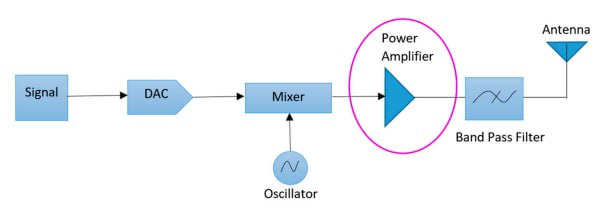
\includegraphics{figures/rf-transmitter-block-diagram.jpeg}
    \caption{Basic block diagram of radio frequency (RF) transmitter \cite{first}.}
    \label{fig:rf-transmitter-block-diagram}
\end{figure}

The development of complementary metal-oxide semiconductor (CMOS) technology, which has greater advantages than gallium arsenide (GaAs) and gallium nitride (GaN) technologies, has led to a rapid increase in the use of wireless communication systems \cite{second,third}. As a result of the compact chip size and ability to operate at a lower power supply, CMOS technology minimizes fabrication costs \cite{fourth} and circuit power dissipation. Radio frequency (RF), digital,
and analog functionalities may be inexpensively combined on a single chip using CMOS \cite{fifth}.
\begin{figure}[h]
    \centering
    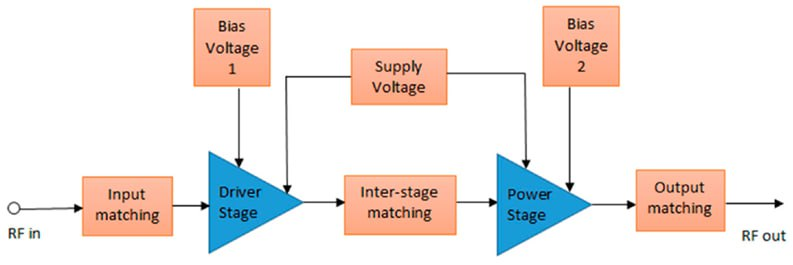
\includegraphics[]{figures/cmos-power-amplifier-block-diagram.jpeg}
    \caption{Block diagram of complementary metal–oxide semiconductor (CMOS) power
amplifier \cite{sixth}.}
    \label{fig:cmos-power-block-diagram}
\end{figure}

For contemporary wireless devices, the CMOS power amplifier (PA) is a potential option to meet the demand for a low-power and low-cost design. In numerous wireless communication applications throughout the years, including home automation, Radio Frequency Identification (RFID), industrial consumer electronics, TV transmissions, phones, and
medical equipment \cite{fourth, fifth, seventh}. CMOS PA has been widely used due to the need for a higher contrast resolution in ultrasonic imaging, which can be achieved by a highly linear PA , it has been integrated in high-frequency medical ultrasonic applications to amplify high-voltage excitation signals to activate ultrasonic transducers \cite{sixth}.

One approach to achieving high efficiency in a wide band power amplifier is to use a two stage amplifier design. In this design, the first stage amplifies the input signal and the second
stage provides additional gain and power. By using a two-stage design, the amplifier can
achieve high efficiency while maintaining good linearity and low distortion \cite{ninth}.

Another approach to achieving high efficiency in a power amplifier is to use a superimposed dual-band configuration. This configuration involves combining two different frequency bands into a single amplifier, which can improve efficiency by reducing the number of
amplifiers required \cite{tenth}.

The use of 90 nm CMOS technology in the design of the power amplifier allows for high levels of integration and miniaturization, making it suitable for use in small devices such as mobile phones and wireless sensors. The use of this technology also enables high levels of
performance in terms of power efficiency and linearity \cite{eleventh}.

\section{Thesis Objectives}
The main objectives of the works are:
\begin{enumerate}[label=\roman*. ]
  \item To increase gain of power amplifier using two stage CMOS power amplifier.
  \item To maintain wideband performance of the amplifier.
  \item To design input and interstage matching network for impedance matching.
\end{enumerate}
 
\section{Context}
The thesis paper titled "Design and of CMOS Power Amplifiers for Enhanced Gain and Bandwidth Using 90 nm CMOS Technology" focuses on the design, simulation, and implementation of a power amplifier that operates in the frequency range of \SI{25}{\giga\hertz} - \SI{35}{\giga\hertz}.

The \SI{25}{\giga\hertz} - \SI{35}{\giga\hertz} frequency range has gained significant attention in various sectors,
including telecommunications, radar systems, and satellite communications. The high frequency range allows for high-speed data transfer and communication, making it suitable
for 5G networks, Internet of Things (IoT), and other wireless applications. Furthermore, the
use of this frequency range is critical in advanced radar systems, such as automotive and
aerospace radar, for precise detection and tracking of objects.

Despite the importance of this frequency range, the design of a power amplifier that meets the
requirements of high power, high efficiency, and wide bandwidth is challenging. The primary
difficulty is the trade-off between power, efficiency, and bandwidth. Increasing the power
amplification often results in lower efficiency, while expanding the bandwidth typically leads
to decreased power output. Moreover, designing a power amplifier that operates in a
superimposed dual-band configuration adds further complexity to the system.

Thus, the statement of the problem situation for this thesis is the difficulty of designing a
power amplifier that meets the requirements of high power, high efficiency, and wide
bandwidth in a superimposed dual-band configuration using 90 nm CMOS technology. The
areas of concern include the selection of an appropriate transistor model, the design of
matching networks, and the optimization of biasing conditions to achieve the desired
performance. The felt need for this research is to provide a solution that overcomes the
challenges of designing a power amplifier for the \SI{25}{\giga\hertz} - \SI{35}{\giga\hertz} frequency range, which is
crucial for many advanced wireless and radar applications.

\section{Significance \& Scope}
\subsection{Significance}
The demand for high-speed wireless communication systems has increased significantly in
recent years. The need for high-frequency wideband power amplifiers (PAs) has become
critical in meeting this demand. The proposed 2-stage high power gain and wideband
(\SI{25}{\giga\hertz} - \SI{35}{\giga\hertz}) power amplifier using superimposed dual-band configuration using 90 nm
CMOS technology aims to address this need. The study is significant in that it provides a
solution for high-frequency wireless communication systems with high gain and
wideband capability.

\subsection{Gap in the Literature}
Although there have been studies on wideband PAs, there is limited research on high frequency wideband PAs using superimposed dual-band configuration.Numerous benefits of CMOS technology include affordability, low power usage, and interoperability with methods used to manufacture integrated circuits. For the creation of power
amplifiers for millimeter-wave applications, it therefore has enormous promise. However,
CMOS power amplifiers struggle to achieve high gain and wide bandwidth due to a number
of challenges, including parasitic capacitances, frequency-dependent transconductance, and
impedance matching problems.

In order to overcome these obstacles and investigate approaches for building and enhancing CMOS power amplifiers, this study will focus on the millimeter-wave frequency range. The main goal is to create power amplifier topologies and strategies that can get around CMOS technology's constraints and provide better performance.

The study's foundational assumptions will be examined, along with the effects of parasitic capacitances and frequency-dependent transconductance on the gain and bandwidth characteristics of CMOS power amplifiers. This research will shed light on the underlying variables affecting the performance of the amplifier and serve as a roadmap for the ensuing design and optimization process.

A multi-stage technique will be used to increase gain and bandwidth, where extra amplifier stages will be cascaded to make up for the shortcomings of individual stages. The frequency response and linearity of the power amplifier will be enhanced by employing a staggered tuning method.

In order to overcome problems with impedance matching, matching networks will be created and implemented into the power amplifier architecture. These networks will make sure that the amplifier and the linked components transmit power effectively, increasing gain and lowering return loss as a result.


\subsection{Scope \& Delimitations}
Numerous benefits of CMOS technology include affordability, low power usage, and interoperability with methods used to manufacture integrated circuits. For the creation of power amplifiers for millimeter-wave applications, it therefore has enormous promise. However, CMOS power amplifiers struggle to achieve high gain and wide bandwidth due to a number of challenges, including parasitic capacitances, frequency-dependent transconductance, and impedance matching problems.

In order to overcome these obstacles and investigate approaches for building and enhancing CMOS power amplifiers, this study will focus on the millimeter-wave frequency range. The main goal is to create power amplifier topologies and methods that can get around CMOS technology's constraints and provide better performance.

\section{Classifications of PA}
\subsection{Class-A, AB, B, and C Power Amplifiers}
The fundamental difference between these four power amplifiers' circuit designs is how they are biased. The class-A power amplifier is demonstrated in Figure \ref{fig:general-topology-PA} to function as a small-signal amplifier, offering linear amplification for the whole input cycle without clipping. As a result, the output closely matches the enlarged input.

However, class-A amplifiers waste power in order to achieve this high level of linearity. The idea of "reduced conduction angle" was developed to increase efficiency while preserving sufficient linearity. In order to implement this idea, active devices are biased with low quiescent current and only partially activated by the input RF signal throughout each cycle.

The amplifier switches from class-AB to class-B and then to class-C by reducing the conduction angle. The active components function as current sources regardless of the conduction angle, giving them the name "transconductance" power amplifiers \cite{twelveth}.

\begin{figure}[h]
    \centering
    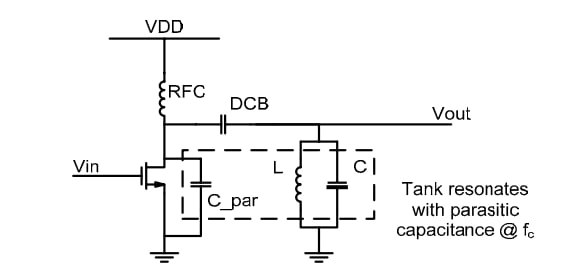
\includegraphics{figures/general-A-B-AB-C.jpeg}
    \caption{A generic topology for class-A, AB, B, and C power amplifiers \cite{twelveth}.}
    \label{fig:general-topology-PA}
\end{figure}

\subsection{Class-D Power Amplifiers}
A class D amplifier is an amplifier that employs a voltage-controlled switch and a filtering tank to amplify a signal. The output tuned network of the amplifier is engineered to exhibit minimal impedance at the fundamental frequency and high impedance at harmonic frequencies. This simplifies the analysis of the amplifier since the drain voltage waveform is straightforward. Under ideal operating conditions, the drain efficiency of the amplifier can reach 100\%, comparable to that of other types of switching power amplifiers \cite{twelveth}.

\begin{figure}[h]
    \centering
    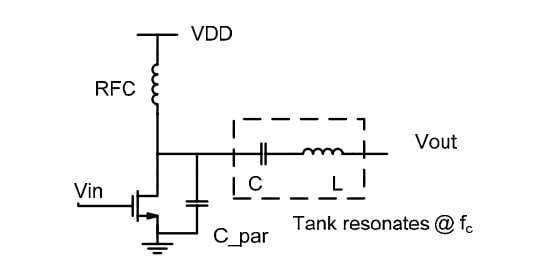
\includegraphics{figures/class-D.jpeg}
    \caption{A voltage switching class-D amplifier \cite{twelveth}.}
    \label{fig:class-D-amplifier}
\end{figure}

\subsection{Class-E Power Amplifier}
The Class-E power amplifier stands out among other switching power amplifiers due to its distinctive capability of incorporating the parasitic capacitances of active devices into wave-shaping and matching networks, resulting in high efficiency. In Figure \ref{fig:class-E-amplifier}, the simplest form of Class-E power amplifiers is depicted, operating by manipulating the drain current and voltage waveforms to prevent overlap. Moreover, the voltage gradually diminishes to zero prior to the activation of the active device, enhancing efficiency by avoiding the charging and discharging of capacitors at the drain. Nevertheless, one limitation of the Class-E power amplifier is its elevated peak voltage.
\begin{figure}[h]
    \centering
    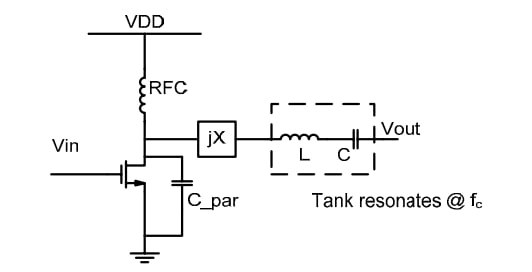
\includegraphics{figures/class-E.jpeg}
    \caption{A simple class-E amplifier \cite{twelveth}}
    \label{fig:class-E-amplifier}
\end{figure}

\subsection{Class-F Power Amplifier}
Class-F amplifiers are recognized for their utilization of a load network that generates resonance at various harmonic frequencies, including the fundamental frequency. Initially, these amplifiers were proposed to enhance the efficiency of overdriven transconductance amplifiers. The active devices employed in class-F amplifiers typically operate as transconductors or current sources.

However, under high input drive conditions, these devices can exhibit switch-like behavior akin to that observed in switching amplifiers. In practical scenarios, it is uncommon to encounter class-F amplifiers with tuned harmonics surpassing the 5th harmonic. This is primarily due to the intricacy associated with designing a waveform shaping network using lumped elements.

\begin{figure}[h]
    \centering
    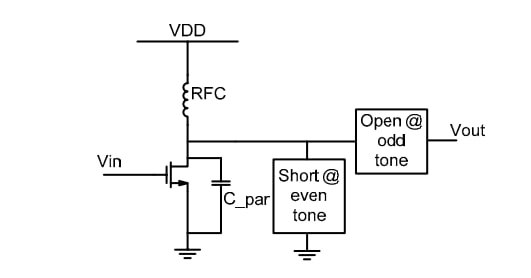
\includegraphics{figures/class-F.jpeg}
    \caption{A class-F power amplifier with tuned harmonics for waveform shaping \cite{twelveth}.}
    \label{fig:my_label}
\end{figure}
\section{Performance Parameter}
Multiple parameters were used to assess the CMOS PA's performance. The output power,
power consumption, power gain, linearity, and power added efficiency (PAE) of a PA design
are its most crucial components. These aspects inevitably come with trade-offs, and as a
result, PA design for CMOS downscaling is difficult. These were the main criteria that were
used for measuring performance.

\subsection{Output Power}
The output power (Pout) \cite{third} is the amount of power sent to the load, which is the antenna. Higher power output must be achieved at the expense of efficiency because some power is lost as heat. To account for this power loss, the device's energy supply must be greater than its needed output power \cite{fourtheen}. The current is essential for maintaining a consistent supply voltage and achieving the necessary output power. As a result, the output power of the power amplifier (PA), which is directly related to the PA's efficiency, determines the PA's performance. The output power is transformed into its appropriate dBm value using the following equation:

\begin{equation}
    P_{out}=\frac{V_{out}^2}{2R_L}
\end{equation}

Where $V_{out}$ denotes the output voltage and $R_L$ denotes the resistance load.
\subsection{Power Consumption}
The power consumption of a power amplifier (PA) is another important aspect of its performance. It's critical to address the need for extended battery life without sacrificing excessive power consumption given the rising demand for portable devices. According to the first equation, the PA's total power consumption ($P_{Total}$) is calculated by adding its dynamic and static power consumption. Leakage current ($I_{CC}$) causes static power consumption $(P_S)$, whereas high-frequency switching causes dynamic power consumption ($P_D$). The two equations that follow show how to determine static and dynamic power usage. Reduced heat generation inside the device is a direct result of reduced static power, which has a major impact on overall power usage. In addition to reducing the device's exposure to heat, this decrease in power consumption increases system dependability. To extend battery life, PAs must use as little electricity as possible because excessive power utilization can reduce their longevity.
\begin{align}
    P_{Total}&=P_S+P_D\\
    P_S&=V_{DD}\times I_{CC}
\end{align}

\begin{equation}
    P_D=\left[\left(C_{pd}\times f_I\times N_{SW}\right)+ \sum \left(C_{Ln}\times f_{On}\right) \right]
\end{equation}

The power consumption capacitance is denoted in the context by $C_{pd}$ (in Farads). In Hertz, $f_I$ stands for the input frequency, while $f_{On}$, also in Hertz, is the total frequency of all outputs at each output. $N_{SW}$ stands for the total number of output switches, and $V_{DD}$ for the supply voltage (in Volts). Additionally, the total load capacitance at each output is represented by $C_{Ln}$.

\subsection{Power Gain}
Power gain ($G$) represents the relationship between output and input power, indicating the power amplifier's ability to deliver a significantly amplified power signal to the load \cite{thirteenth}. It quantifies the extent to which the amplifier increases the amplitude of a signal. By enhancing the output power, a power amplifier aims to enhance efficiency and sensitivity.
\begin{equation}
    G=10\log_{10}\left(\frac{P_{out}}{P_{in}}\right) \quad [dB]
\end{equation}

Here, $P_{out}$ is the output power and $P_{in}$ is the input power.

\subsection{Efficiency}
Power amplifiers (PAs) have two types of efficiency: drain efficiency (DE) and power-added efficiency (PAE). RF output power to DC power dissipation is measured as DE \cite{fifteenth}. By subtracting the output power obtained from the input power and dividing the result by the DC power dissipation, PAE is determined. The input power is examined by PAE to determine how well the PA transforms DC power into an AC power signal. When the output power is higher, a higher PAE is attained \cite{fifteenth}. 
\begin{align}
    DE=\frac{P_{out}}{P_{DC, drain}}\\
    PAE=\frac{P_{out}-P_{in}}{P_{DC, drain}}
\end{align}

\subsection{Linearity}
Linearity refers to the condition where the output of a device changes in a linear manner in response to changes in the input signal \cite{sixteen}. In modern RF communication systems, achieving high linearity is increasingly crucial. Typically, linearity is evaluated based on the third-order intercept point (IP3) value. The IP3 is determined by plotting the output power against the input power on a logarithmic scale \cite{sixteen}. A higher linearity implies that the obtained output power is directly proportional to the input power.

To fulfill the requirements of current applications, power amplifiers (PAs) need to be designed with low power consumption, high output power, high power gain, high power-added efficiency (PAE), and good linearity. The power delivered by a PA and its PAE are significant factors in PA design, as they directly impact the overall performance and efficiency.
\section{Thesis Outline}
In chapter 2, we discussed overview of CMOS power amplifier and the literature review.

In chapter 3, we discussed the common source, common-gate power amplifier 3-dB frequency and provided an explanation of the research methodology. Additionally, we employ the stagger tuning technique to create a CMOS power amplifier.

We presented the simulation results for single-stage and dual-stage power amplifiers in chapter 4. We examined the simulation's output results and cross-checked them against previously published research.

The conclusions to the thesis were determined in chapter 5, and subsequent works were also discussed. 
\chapter{LITERATURE REVIEW}
\section{Overview of CMOS Power Amplifier}
A power amplifier employing complementary metal-oxide semiconductor (CMOS) technology is a type of electrical circuit. It is essential to many applications, including satellite communication, Wi-Fi, Bluetooth, and wireless communication networks like cellular networks.

In comparison to alternative amplifier technologies, CMOS power amplifiers provide a number of benefits, including high integration density, low power consumption, and compatibility with traditional CMOS processes. They are very appealing for usage in portable and low-power devices where cost effectiveness and power efficiency are crucial.

A power amplifier's main job is to boost an input signal's power level to a level appropriate for transmission or driving a load. This is accomplished in the case of CMOS power amplifiers by using CMOS transistors as the amplifying components. Input matching networks, gain stages, and output matching networks are common stages in the architecture of CMOS power amplifiers.

Power transfer is optimized by the input matching network's role in impedance matching between the amplifier and the stage before it. By doing this, it makes sure that the majority of the signal power is absorbed by the amplifier as opposed to being reflected back to the source. In addition to enhancing signal fidelity and reducing distortion, proper impedance matching.

The gain stages, which magnify the input signal to the appropriate output power level, are the heart of the power amplifier. They are made to offer high gain with a focus on linearity and low distortion. The inherent constraints of CMOS technology at high frequencies can make achieving high gain in CMOS power amplifiers difficult. Performance characteristics of the amplifier, such as power gain, bandwidth, and linearity, are influenced by parasitic capacitances and resistances in CMOS transistors.

Different design strategies are used to lessen these restrictions. The performance of the amplifier can be enhanced through careful device sizing, layout optimization, the use of inductive components, and matching networks. To attain the needed performance at high frequencies, strategies like cascode designs, impedance modification, and distributed amplifiers are used.

In order to maximize power transfer to the load, the output matching network guarantees impedance matching between the power amplifier and the load. It is essential for effectively supplying electricity and reducing reflections that can reduce the signal quality.

A thorough understanding of circuit theory, RF (Radio Frequency) design, and CMOS device characteristics is required while designing a CMOS power amplifier. The performance of the amplifier is modeled and examined using sophisticated simulation tools and optimization techniques, taking into consideration several factors like gain, power efficiency, linearity, and bandwidth.

CMOS power amplifiers can be designed for various frequency ranges, from low-frequency applications to mm-wave frequencies. The design considerations and techniques vary depending on the targeted frequency range and application requirements. High-frequency CMOS power amplifiers often require careful consideration of the parasitic elements, transmission line effects, and the use of advanced circuit topologies and techniques.

Ongoing research and advancements in CMOS power amplifier design aim to push the boundaries of performance. Researchers are exploring novel architectures, device structures, and circuit topologies to achieve higher power efficiency, wider bandwidth, improved linearity, and integration with other circuit blocks.

In conclusion, CMOS power amplifiers provide power amplification with good efficiency, compactness, and compatibility with typical CMOS processes, making them an attractive option for integrated circuit designs. They are essential parts of contemporary wireless communication systems because they permit faster data rates, greater energy economy, and more functionality.

\section{Existing Power Amplifier Design Techniques}
 CMOS technology possesses the ability to incorporate highly intricate digital circuitry, providing exceptional versatility and cost-effectiveness by integrating an entire radio system on a single chip. However, when it comes to power amplifier (PA) design, CMOS implementation poses significant challenges due to inherent limitations in standard CMOS processes from an RF perspective. These limitations include low oxide breakdown voltage, limited current drive capability, substrate coupling, and subpar quality and tolerance of on-chip passive components \cite{1320534, 1635249, 1465784}. These disadvantages have a detrimental impact on PA performance, particularly in terms of output power, efficiency, and linearity.
 
 High-data-rate and wide-bandwidth (BW) capabilities are required due to the growing need for wideband radio frequency (RF) transceivers in radar and satellite communication systems at sub-mm wave bands. At these higher frequencies, however, constructing wideband power amplifiers (PAs) with high power added efficiency (PAE) utilizing CMOS technologies is quite difficult \cite{8886521, 8354388, 9354447}.
Single broadband power amplifiers (PA) that can enable ultra-high data rate modulation and concurrently amplify multiple carriers are becoming more and more necessary in contemporary communication systems. The necessity for the PA to operate over a wider bandwidth than traditional narrowband amplifiers can be found in a number of applications, including imaging systems \cite{4977464}.

A popular and efficient method for achieving wideband features is the use of staggered power amplifiers (PAs) \cite{8678458, sapawl2012}. To achieve staggered wideband performance, this method includes designing the driver and main stages at two different center frequencies.

A low-power, full-band, low-noise amplifier for ultra-wideband receivers is described in study \cite{5497167}. For use in ultra-wideband applications, a low-power full-band low-noise amplifier (FB-LNA) is given. A MEMS tunable bandpass filter operating in the K band is described in Paper \cite{5728610}. It has a tiny dimension of 2.9 mm by 1.5 mm, a large continuous tuning range of 32\%, and a low insertion loss of -2.79-3.58 dB. It is suggested to use a straightforward CMOS broadband power amplifier architecture with great linearity and decent efficiency. To achieve a wider bandwidth from 0.9 to 3.5 GHz and low power consumption, the proposed power amplifier design used a staggered tuning technique composed of two stages of amplifier with distinct resonance frequencies \cite{sapawl2012}. An ultra-wideband (UWB) low-noise amplifier (LNA) employing a noise-cancelling approach and the TSMC 0.18-m RF CMOS technology is shown in paper \cite{shim2013}. In \cite{7202869}, a new method for designing transimpedance amplifiers (TIAs) that makes use of inverted transformer coils and stagger tuning is presented. In the paper \cite{7348667}, an inductorless 10 Gbps automatic gain control (AGC) circuit with speed-enhanced variable gain amplifiers (VGA), unique exponential function generators for extended linear performance in dB, power detectors and a comparator are presented. In paper \cite{8400821}, a T-type network and pole-tuning methods are used to study a broadband CMOS amplifier in the d band. a brand-new pole-tuning method using a T-type network to increase interstage bandwidth The stagger tuning technique is proposed in Paper \cite{8939351} at two separate frequencies, with an inductance of four stages selected to match the pole frequency at a lower frequency ($f_L$) and an inductance of the remaining four stages selected for the upper frequency ($f_H$). Citation \cite{9829838} states that the paper describes a two-stage CMOS 180-nm wideband power amplifier (PA). The PA uses defected-ground-structure (DGS) inductors and a superimposed staggered method. To produce a flat gain response throughout the full bandwidth, the design consists of a superimposed dual-band (SDB) driver stage and a wideband peaking main stage at the center frequency. By lowering insertion losses in the matching circuits, the usage of DGS inductors contributes to an improvement in PAE. With a chip area of 0.564 ${mm}^2$, the installed PA shows a power boost of 12 dB. It reaches a high fractional bandwidth (FBW) of 44.4\% at the center frequency and a saturated output power of 16.6 dBm.
\chapter{METHODOLOGY}
The methodology of this work is
\tikzstyle{startstop} = [rectangle, rounded corners, 
minimum width=3cm, 
minimum height=1cm,
text centered, 
draw=black, 
fill=red!30]

\tikzstyle{io} = [trapezium, 
trapezium stretches=true, % A later addition
trapezium left angle=70, 
trapezium right angle=110, 
minimum width=3cm, 
minimum height=1cm, 
text centered, 
text width=3cm,
draw=black, fill=blue!30]

\tikzstyle{process} = [rectangle, 
minimum width=3cm, 
minimum height=1cm, 
text centered, 
text width=3cm, 
draw=black, 
fill=orange!30]

\tikzstyle{decision} = [diamond, 
minimum width=3cm, 
minimum height=1cm, 
text centered,
text width=3cm,
draw=black, 
fill=green!30]
\tikzstyle{arrow} = [thick,->,>=stealth]

\begin{figure}
    \centering
    \begin{tikzpicture}[node distance=2cm]
    \node (start) [startstop] {Start};
    \node (in1) [io, below of=start] {Determine specifications: Frequency range, Gain};
    \node (in2) [io, below of=in1] {Select the transistor};
    \node (process1) [process, below of=in2] {Design the first stage Amplifier};
    \node (process2) [process, below of=process1] {Design the second stage Amplifier};
    \node (process3) [process, below of=process2] {Design the inter-stage matching network.};
    \node (process4) [process, below of=process3] {Design the input matching network.};
    \node (process5) [process, below of=process3] {Design the input matching network.};
    \node (process6) [process, below of=process5] {Simulate and optimize the design};
    \node (dec1) [decision, right of=process6, xshift=3cm] {Meet specifications?};
    \node (out1) [io, right of=dec1, xshift=3cm] {Output};
    \node (stop) [startstop, below of=out1] {Stop};
    \draw [arrow] (start) -- (in1);
    \draw [arrow] (in1) -- (in2);
    \draw [arrow] (in2) --(process1);
    \draw [arrow] (process1) -- (process2);
    \draw [arrow] (process2) -- (process3);
    \draw [arrow] (process3) -- (process4);
    \draw [arrow] (process4) -- (process5);
    \draw [arrow] (process5) -- (process6);
    \draw [arrow] (process6) -- (dec1);
    \draw [arrow] (dec1) -- node[anchor=south] {yes} (out1);
    \draw [arrow] (dec1) |- node[anchor=south] {no} (process1);
    \draw [arrow] (out1) -- (stop);
\end{tikzpicture}
    \caption{Design methodology of this work.}
    \label{fig:methodology-flow-chart}
\end{figure}

\begin{enumerate}[label=\roman*. ]
    \item Determine the specifications: The initial step is to ascertain the PA's specs, such as the appropriate frequency range, output power, and gain.
    \item Select the transistor: Choose the right transistor for the amplifier based on the requirements. A CMOS transistor was used in this instance because it is appropriate for high-frequency applications.
    \item Design the first stage: The amplifier's first stage is built to deliver the appropriate gain. The stagger tuning approach should be used to build this stage, which entails changing the inductors and capacitors so that the input and output resonant frequencies are not the same. The amplifier's bandwidth is widened using this method.
    \item Design the second stage: In order to provide more gain and bandwidth, the second stage of the amplifier should likewise be developed using a stagger tuning technique.
    \item Design the input matching network: Create an input matching network to match the transistor's impedance with the source impedance. A network for matching lumped elements can be used to accomplish this.
    \item Design the interstage matching network: Create an interstage matching network to match the first and second stages' impedances.
    \item Design the output matching network: Create an output matching network to match the amplifier's impedance with the load's impedance.
    \item Simulate and optimize the design: Use a circuit simulator (Cadence virtuoso and ADS) to simulate and improve the design, then adjust component values for optimum performance.
\end{enumerate}

\section{Superimposed Dual Band Power Amplifier}
\subsection{High Frequency MOSFET Model}
The MOSFET's small-signal model, which includes the four capacitances $C_{gs}$, $C_{gd}$, $C_{sb}$, and $C_{db}$, is depicted in Figure \ref{fig:mosfet-high-frequecy-model}. MOSFET amplifier's high-frequency response can be predicted using this approach. The model is significantly simplified when the source is coupled to the body, as shown in Figure \ref{fig:mosfet-source-connected-to-bodyl}. Though $C_{gd}$ is small in our model, $C_{gd}$ has a substantial impact on how amplifiers respond at high frequencies, necessitating its inclusion. On the other hand, capacitance $C_{db}$ can typically be disregarded, greatly simplifying manual analysis. Figure \ref{fig:mosfet-neglected-Cdb} depicts the resulting circuit. Finally, we display the high-frequency T model in its simplified form in Figure \ref{fig:mosfet-equivalent-t-model}.
\begin{figure}[h]
    \centering
    \begin{circuitikz}[american, scale=.8, thick]
    \draw (0,0) node[left, above]{$G$} to[short, o-] ++(2,0) coordinate(A)
    to[C, l=$C_{gd}$] ++(4,0) coordinate(B)
    to[short] ++(3,0) coordinate(C)
    to[short] ++(3,0) coordinate(D)
    to[R, l=$r_0$, *-] ++(0,-4) -- ++(-7,0) coordinate(E) -- ++(-2,0) coordinate(F) -- ++(-1,0)
    ;
    \draw (A) to[C, l=$C_{gs}$, v_>=$V_{gs}$, *-] ++(0,-4);
    \draw (B) to[cI, l^=$g_mV_{gs}$, *-*] ++(0,-4);
    \draw (C) to[cI, l^=$g_mV_{bs}$, *-*] ++(0,-4);
    \draw (D) to[short] ++(2,0) coordinate(H) to[short, -o] ++(1,0) node[right, above]{$D$};
    \draw (E) to[C, l=$C_{sb}$, v_<=$V_{bs}$, *-] ++(0,-2) coordinate(G)
               to[short, -o] ++(0, -0.5) node[left, below]{$B$};
    \draw (F) to[short, *-o] ++(0, -2.5) node[left, below]{$S$};
    \draw (H) to[C, l=$C_{db}$, *-] ++(0, -6) to[short, -*] (G); 
\end{circuitikz}
    \caption{MOSFET equivalent-circuit model at high frequencies.}
    \label{fig:mosfet-high-frequecy-model}
\end{figure}

\begin{figure}[h]
    \centering
    \begin{circuitikz}[american, scale=1, thick]
    \draw (0,0) node[left, above]{$G$} to[short, o-] ++(1,0) coordinate(A)
    to[C, l=$C_{gd}$] ++(4,0) coordinate(B)
    to[short] ++(3,0) coordinate(C)
    to[short] ++(3,0) coordinate(D)
    to[R, l=$r_0$, *-] ++(0,-4) -- ++(-8,0) coordinate(E) -- ++(-2,0);
    \draw (A) to[C, l=$C_{gs}$, v_>=$V_{gs}$, *-] ++(0,-4);
    \draw (B) to[cI, l^=$g_mV_{gs}$, *-*] ++(0,-4);
    \draw (C) to[cI, l^=$g_mV_{bs}$, *-*] ++(0,-4);
    \draw (D) to[short] ++(2,0) coordinate(H) to[short, -o] ++(1,0) node[right, above]{$D$};
    \draw (H) to[C, l=$C_{db}$, *-] ++(0,-4)-- ++(-2,0);
    \draw (E) to[short, *-o] ++(0, -0.8) node[left, below]{$S$};
\end{circuitikz}
    \caption{The corresponding circuit for the scenario when the source is attached to the substrate (body).}
    \label{fig:mosfet-source-connected-to-bodyl}
\end{figure}

\begin{figure}[h]
    \centering
    \begin{circuitikz}[american, scale=1, thick]
    \draw (0,0) node[left, above]{$G$} to[short, o-] ++(1,0) coordinate(A)
    to[C, l=$C_{gd}$] ++(4,0) coordinate(B)
    to[short] ++(3,0) coordinate(C)
    to[short] ++(3,0) coordinate(D)
    to[R, l=$r_0$, *-] ++(0,-4) -- ++(-8,0) coordinate(E) -- ++(-2,0) coordinate(F);
    \draw (A) to[C, l=$C_{gs}$, v_>=$V_{gs}$, *-] ++(0,-4);
    \draw (B) to[cI, l^=$g_mV_{gs}$, *-*] ++(0,-4);
    \draw (C) to[cI, l^=$g_mV_{bs}$, *-*] ++(0,-4);
    \draw (D) to[short, -o] ++(1,0) node[right, above]{$D$};
    \draw (E) to[short, *-o] ++(0, -.6) node[left, below]{$S$};
\end{circuitikz}
    \caption{The equivalent-circuit model of Figure \ref{fig:mosfet-source-connected-to-bodyl} without $C_{db}$ (to make analysis simpler).
}
    \label{fig:mosfet-neglected-Cdb}
\end{figure}

\begin{figure}[h]
    \centering
    \begin{circuitikz}[american, scale=1, thick]
    \draw (0,0) node[above, right]{$D$} to[short, o-] ++(0,-1) coordinate(A)
    to[cI, l^=$g_mV_{gs}$, *-*] ++(0,-3) coordinate(B)
    to[R, l=$\frac{1}{g_m}$, -*] ++(0,-2) coordinate(C)
    to[short, -o] ++(0,-1) node[below, left]{$S$};
    \draw (B) to[short, -o] ++(-3,0) node[right, above]{$G$};
    \draw (A) -- ++(-2,0) to[C, l=$C_{gd}$] ++(0,-3);
    \draw (C) -- ++(-2,0) to[C, l=$C_{gs}$, v_<=$V_{gs}$, -*] ++(0,2);
\end{circuitikz}
    \caption{The simplified high-frequency T model.}
    \label{fig:mosfet-equivalent-t-model}
\end{figure}

\subsection{High Frequecy Response of CS Power Amplifier}

The common-source amplifier is represented by a thorough high-frequency equivalent circuit in Figure \ref{fig:common-source-high-frequency}. The total resistance in this circuit, $R'_L$, which includes $R_D$, $r_o$, and $R_L$ (if applicable), is measured between the output node (drain) and ground.
\begin{figure}[h]
    \centering
    \begin{circuitikz}[american, scale=1, thick]
        \draw (0,0) node[left]{$IN$} to[short, o-] ++(0.5,0)
      to[C, l=$C_s$] ++(2,0) -- ++(1,0) coordinate(E) -- ++(1,0) coordinate(G) -- ++(1,0) node[nigfete, anchor=G](mos3){$M_1$}
        (mos3.S)-- ++(0, -2) coordinate(gnd) node[ground]{}
        (mos3.D) to[short] ++(0,1) coordinate(D) to[R, l=$R_D$] ++(0,2) node[vcc]{$V_{DD}$};
        \draw (E) to[R, l=$R_1$] ++(0,2.5) node[vcc]{$V_{G1-CS}$};
        \draw (G) to[C, l_=$C_{gs}$] ++(0,-2.5) to[short, -*] (gnd);
        \draw (G) to[C, l_=$C_{gd}$, *-] ++(0,2) to[short, -*] (D);
        \draw (D) -- ++(2,0) coordinate(out1) to[R, l=$R'_L$] ++(0,-2) node[ground]{};
        \draw (out1) -- ++(2,0) coordinate(out) to[C, l=$C_L$] ++(0,-2) node[ground]{};
       \draw (out) to[short, -o] ++(0.5,0)node[right]{$OUT$};

    \end{circuitikz}
    \caption{Common-source power amplifier circuit at high frequency.}
    \label{fig:common-source-high-frequency}
\end{figure}

A current-source load, an extra amplifier stage's input capacitance (if applicable), and a MOSFET's drain-to-body capacitance ($C_db)$ are all included in the total capacitance between the drain node and ground, which is denoted by the symbol $C_L$.

We use the open-circuit time constants method to determine the 3-dB frequency $f_H$ of the CS amplifier depicted in Figure \ref{fig:cs-equivalent-high-frequency}. In order to accomplish this, we set input signal equal to zero and examine each of the four capacitances separately, leaving the other three at zero.
\begin{figure}
    \centering
    \begin{circuitikz}[american, scale=1, thick]
    \draw (0,0) node[ground]{} to[american voltage source, invert] ++(0,2)
    -- ++(0.5,0) to[C, l=$C_s$] ++(2,0) -- ++(.5,0) coordinate(A) -- ++(2,0)coordinate(B) -- ++(0.5,0) to[C, l=$C_{gd}$] ++(2,0) -- ++(0.5,0) coordinate(C)
    to[cI, l_=$g_mV_{gs}$, *-] ++(0,-2) node[ground]{};
    \draw (C) -- ++(2,0) coordinate(D) to[C, l=$C_L$, *-] ++(0,-2) node[ground]{};
    \draw (D) -- ++(2,0) to[R, l=$R'_L$] ++(0,-2)node[ground]{};
    \draw (A) to[R, l=$R_G$, *-] ++(0,-2)node[ground]{};
    \draw (B) to[R, l=$C_{gs}$, *-] ++(0,-2)node[ground]{};
\end{circuitikz}
    \caption{The CS power amplifier, a high frequency equivalent circuit shown in Figure \ref{fig:common-source-high-frequency}.}
    \label{fig:cs-equivalent-high-frequency}
\end{figure}
The circuit depicted in Figure \ref{fig:tau_cn_tau_gs_CS} illustrates the configuration used to calculate the resistance $R_s$, which is the effective resistance seen by $C_s$. It can be expressed as 
\begin{align}
    R_s &=R_G\\
    \tau_c &=R_GC_s
\end{align}
On the other hand, Figure \ref{fig:tau_gs_cs} presents the circuit used to determine $R_{gs}$ seen by $C_{gs}$.
\begin{align}
    R_{gs}&=R_G\\
    \tau_{gs}&=R_GC_{gs}
\end{align}
\begin{figure}[h]
  \centering
  \begin{subfigure}[b]{0.49\textwidth}
  \centering
    \begin{circuitikz}[american, scale=1, thick]
    \draw (0,0)node[left]{$G$} to[short, o-] ++(1,0) to[R, l=$R_G$] ++(0,-2) node[ground]{};
    \draw [->] ++(-0.5,-2.5) node[below]{$R_s$} -- ++(0, 1.5) -- ++(1,0);
\end{circuitikz}
    \caption{}
    \label{fig:tau_c_cs}
  \end{subfigure}
  \hfill
  \begin{subfigure}[b]{0.49\textwidth}
  \centering
    \begin{circuitikz}[american, scale=1, thick]
    \draw (0,0)node[right]{$G$} to[short, o-] ++(-1,0) to[R, l_=$R_G$] ++(0,-2) node[ground]{};
    \draw [->] ++(0.5,-2.5) node[below]{$R_{gs}$} -- ++(0, 1.5) -- ++(-1,0);
\end{circuitikz}
    \caption{}
    \label{fig:tau_gs_cs}
  \end{subfigure}

  \caption{Applying the open-circuit time-constants approach to Figure \ref{fig:cs-equivalent-high-frequency} and determine $\tau_s$ and $\tau_{gs}$.
}
  \label{fig:tau_cn_tau_gs_CS}
\end{figure}
In Figure \ref{fig:tau_l_cs} illustrates the configuration used to calculate the resistance $R_l$, which is the effective resistance seen by $C_L$. It can be expressed as 
\begin{align}
    R_l &=R'_L \quad \text{where, } R'_L=\left(R_L||R_D||r_0\right)\\
    \tau_l &=R'_LC_L=\left(R_L||R_D||r_0\right)C_L
\end{align}. 
On the other hand, Figure \ref{fig:tau_gd_cs} presents the circuit used to determine $R_{gd}$ seen by $C_{gd}$.
\begin{align}
    R_{gd}&=\frac{V_x}{I_x}=R_G\left(1+g_mR'_L\right)+R'_L\\
    \tau_{gs}&=R_{gd}C_{gd}=\left[R_G\left(1+g_mR'_L\right)+R'_L\right]C_{gd}
\end{align}
Thus the effective time constant $\tau_H$ can be found as
\begin{align}
    \tau_H&=\tau_s + \tau_{gs} + \tau_l +\tau_{gd}\\
    &=R_GC_s+R_GC_{gs}+\left(R_L||R_D||r_0\right)C_L+\left[R_G\left(1+g_mR'_L\right)+R'_L\right]C_{gd}
\end{align}
\begin{figure}[h]
  \centering
  \begin{subfigure}[b]{0.49\textwidth}
  \centering
    \begin{circuitikz}[american, scale=1, thick]
    \draw (0,0) to[short, o-] ++(-1,0) coordinate(A) -- ++(-2,0)
    to[cI, l=$g_mV_{gs}$] ++(0,-2) node[ground]{};
    \draw (A) to[R, l=$R'_L$] ++(0,-2) node[ground]{};
    \draw [->] ++(0.5,-2.5) node[below]{$R_{l}$} -- ++(0, 1.5) -- ++(-.6,0);
\end{circuitikz}
    \caption{}
    \label{fig:tau_l_cs}
  \end{subfigure}
  \hfill
  \begin{subfigure}[b]{0.49\textwidth}
  \centering
   \begin{circuitikz}[american, scale=1, thick]
    \draw (0,0) node[ground]{} to[R, l=$R_G$] ++(0,2)-- ++(0.5,0)
    to[I, l_=$I_x$, v^<=$V_x$] ++(2,0) -- ++(0.5,0) coordinate(D)
    to[cI, l=$g_mV_{gs}$] ++(0,-2)node[ground]{};
    \draw (D) -- ++(2,0) to[R, l=$R'_L$] ++(0,-2) node[ground]{};
\end{circuitikz}
    \caption{}
    \label{fig:tau_gd_cs}
  \end{subfigure}

  \caption{Applying the open-circuit time-constants approach to Figure \ref{fig:cs-equivalent-high-frequency} and determine $\tau_l$ and $\tau_{gd}$.
}
  \label{fig:tau_l_tau_gd_CS}
\end{figure}

and the 3-db frequency $\omega_H$ is
\begin{equation}
    \omega_H=\frac{1}{R_GC_s+R_GC_{gs}+\left(R_L||R_D||r_0\right)C_L+\left[R_G\left(1+g_mR'_L\right)+R'_L\right]C_{gd}}
\end{equation}

\subsection{High Frequency Response of CG Power Amplifier}
In Figure \ref{fig:common-gate-high-frequency}, the CG amplifier is depicted with the MOSFET internal capacitances, $C_{gs}$ and $C_{gd}$, separated from the model and highlighted. A capacitance $C_L$ is inserted at the output node to reflect the combined effect of the output capacitance of a current-source load and the input capacitance of a later amplifier stage in order to take into account various aspects. The MOSFET capacitance, $C_db$, is included in this capacitance, $C_L$.
\begin{figure}[h]
    \centering
    \begin{circuitikz}[american, scale=1, thick]
        \draw (0,0) node[ground]{} to[short] ++(0.5,0)
      to[C, l=$C_s$] ++(2,0) -- ++(1,0) coordinate(E) -- ++(1,0) coordinate(G) -- ++(1,0) node[nigfete, anchor=G](mos3){$M_1$}
        (mos3.S)-- ++(0, -1) coordinate(gnd) -- ++(0,-1) to[R, l=$R_s$] ++(-2,0) -- ++(-0.5,0) to[esource, l_=$RF_{in}$] ++(0,-2) node[ground]{} 
        (mos3.D) to[short] ++(0,1) coordinate(D) to[L, l=$L_D$] ++(0,2) node[vcc]{$V_{DD}$};
        \draw (E) to[R, l=$R_1$] ++(0,2.5) node[vcc]{$V_{G1-CG}$};
        \draw (G) to[C, l_=$C_{gs}$] ++(0,-1.5) to[short, -*] (gnd);
        \draw (G) to[C, l_=$C_{gd}$, *-] ++(0,2) to[short, -*] (D);
        \draw (D) -- ++(2,0) coordinate(out1) to[R, l=$R_L$] ++(0,-2) node[ground]{};
        \draw (out1) -- ++(2,0) coordinate(out) to[C, l=$C_L$] ++(0,-2) node[ground]{};
       \draw (out) to[short, -o] ++(0.5,0)node[right]{$OUT$};
    \end{circuitikz}
    \caption{Common-gate power amplifier circuit at high frequency.}
    \label{fig:common-gate-high-frequency}
\end{figure}
\begin{figure}[h]
    \centering
    \begin{circuitikz}[american, scale=1, thick]
        \draw(0,0) node[ground]{}
        to[C, l=$C_s$] ++(0,2) -- ++(1.5,0) coordinate(G) -- ++(1.5,0) coordinate(G1)
        to[C, l=$C_{gs}$] ++(0,-2) -- ++(1.5,0) coordinate(S) -- ++(1.5,0)
        to[cI, l=$g_mV_{gs}$, invert, *-] ++(0,2) coordinate(D1) -- ++(2,0) coordinate(D) -- ++(1.5,0) coordinate(A) -- ++(1.5,0) coordinate(B) -- ++(1.5,0)
        to[L, l=$L$] ++(0,-2) node[ground]{};
        \draw (G1) to[C, l=$C_{gd}$, *-*] (D1);
        \draw (G) to[R, l=$R_G$, *-] ++(0,-2) node[ground]{};
        \draw (D) to[R, l=$r_0$, *-] ++(0,-2)-- ++(-2,0);
        \draw (A) to[R, l=$R_L$, *-] ++(0,-2) node[ground]{};
        \draw (B) to[C, l=$C_L$, *-] ++(0,-2) node[ground]{};
        \draw (S) to[short, *-] ++(0,-1)
        to[R, l=$R_s$] ++(-2,0)
        to[esource, l_=$RF_{in}$] ++(0,-2) node[ground]{};
    \end{circuitikz}
    \caption{High frequency equivalent circuit for the CG power amplifier shown in Figure \ref{fig:common-gate-high-frequency}.}
    \label{fig:cg-equivalent-high-frequency}
\end{figure}
We use the open-circuit time constants method to determine the 3-dB frequency $f_H$ of the
CG amplifier depicted in Figure \ref{fig:cg-equivalent-high-frequency}. In order to accomplish this, we set input signal equal to
zero and examine each of the four capacitances and one inductor separately, leaving the other four at zero.

The circuit depicted in Figure \ref{fig:tau_c_cg} illustrates the configuration used to calculate the resistance $R_c$, which is the effective resistance seen by $C_s$. It can be expressed as 
\begin{align}
    R_c&=R_G\\
    \tau_c& =R_G C_s 
\end{align}

On the other hand, Figure \ref{fig:tau_gs_cg} presents the circuit used to determine $R_{gs}$ seen by $C_{gs}$.
\begin{align}
    R_{gs} &=\frac{V_x}{I_x}=R_G\left(1+g_m\left(R_s||r_0\right)\right)+R_s||r_0\\
    \tau_{gs} &=R_{gs}C_{gs}\\
    &=\left[R_G\left(1+g_m\left(R_s||r_0\right)\right)+\left(R_s||r_0\right) \right]C_{gs}
\end{align}
\begin{figure}[h]
  \centering
  \begin{subfigure}[b]{0.49\textwidth}
  \centering
    \begin{circuitikz}[american, scale=1, thick]
    \draw (0,0)node[left]{$G$} to[short, o-] ++(1,0) to[R, l=$R_G$] ++(0,-2) node[ground]{};
    \draw [->] ++(-0.5,-2.5) node[below]{$R_c$} -- ++(0, 1.5) -- ++(1,0);
\end{circuitikz}
    \caption{}
    \label{fig:tau_c_cg}
  \end{subfigure}
  \hfill
  \begin{subfigure}[b]{0.5\textwidth}
  \centering
    \begin{circuitikz}[american, scale=.9, thick]
        \draw (0,0) node[ground]{}
        to[R, l=$R_G$] ++(0,2) -- ++(2,0)
        to[I, l_=$I_x$, v^<=$V_x$] ++(0,-2) -- ++(1.5,0) coordinate(S) -- ++(1.5,0) coordinate(A)
        to[cI, l=$g_mV_{gs}$, invert] ++(0,2) -- ++(1.5,0) coordinate(B)
        to[R, l=$r_0$] ++(0,-2) -- (A);
        \draw (S) to[short, *-] ++(0, -1)
        to[R, l=$R_s$] ++(-2,0) node[ground]{};
        \draw (B) -- ++(1.5,0) coordinate(C) -- ++(1.,0) -- ++(0,-2) node[ground]{};
        \draw (C) to[R, l=$R_L$] ++(0,-2) node[ground]{};
    \end{circuitikz}
    \caption{}
    \label{fig:tau_gs_cg}
  \end{subfigure}
  \caption{Applying the open-circuit time-constants method, find $\tau_c$ and $\tau_{gs}$ for the CG equivalent circuit shown in Figure \ref{fig:cg-equivalent-high-frequency}.
}
  \label{fig:tau_c_tau_gs_CS}
\end{figure}

In Figure \ref{fig:tau_gd_cg} illustrates the configuration used to calculate the resistance $R_{gd}$, which is the effective resistance seen by $C_{gd}$. It can be expressed as 
\begin{align}
    R_{gd}&=\frac{V_x}{I_x}=R_G\left(1+g_mR'_L\right)+R'_L \quad \text{where, } R'_L=R_s||r_0\\
    \tau_{gd}&=\left[R_G\left(1+g_mR'_L\right)+R'_L \right]C_{gd}
\end{align}

Similarly, Figure \ref{fig:tau_l_cg} presents the circuit used to determine $R_{l}$ seen by $C_{L}$.
\begin{align}
    R_l&=\frac{V_x}{I_x}=0\\
    \tau_L &=R_lC_L=0
\end{align}
\begin{figure}[h]
  \centering
  \begin{subfigure}[b]{0.49\textwidth}
  \centering
    \begin{circuitikz}[american, scale=1, thick]
    \draw (0,0) node[ground]{}
    to[R, l=$R_G$] ++(0,2) 
    to[I, l_=$I_x$, v^<=$V_x$] ++(3,0) coordinate(D)
    to[cI, l=$g_mV_{gs}$, *-*] ++(0,-2) coordinate(S)
    to[R, l=$R_s$] ++(-2,0) node[ground]{};
    \draw (D) -- ++(2,0) coordinate(E) 
    to[R, l=$r_0$, *-] ++(0,-2) -- (S);
    \draw (E) -- ++(1,0) node[ground]{};
    \end{circuitikz}
    \caption{}
    \label{fig:tau_gd_cg}
  \end{subfigure}
  \hfill
  \begin{subfigure}[b]{0.49\textwidth}
  \centering
    \begin{circuitikz}[american, scale=1, thick]
         \draw (0,0) node[ground]{} to[R, l=$R_s$] ++(2,0)
         to[cI, l=$g_mV_{gs}$, invert, *-] ++(0,2) -- ++(2,0) coordinate(A)
         to[R, l_=$r_0$, *-] ++(0,-2) -- ++(-2,0);
         \draw (A) -- ++(1.5,0) coordinate(B) 
         to[R, l_=$R_L$, *-] ++(0,-2) node[ground]{};
         \draw (B) -- ++(1.5,0) coordinate(C)
         to[I, l_=$I_x$, v^>=$V_x$, invert, *-] ++(0,-2) node[ground]{};
         \draw (C) -- ++(1,0) node[ground]{};
    \end{circuitikz}
    \caption{}
    \label{fig:tau_l_cg}
  \end{subfigure}
  \caption{Applying the open-circuit time-constants method, find $\tau_{gd}$ and $\tau_{L}$ for the CG equivalent circuit shown in Figure \ref{fig:cg-equivalent-high-frequency}.
}
  \label{fig:tau_gd_tau_l_CS}
\end{figure}

On the other hand, Figure \ref{fig:tau_d_cg} presents the circuit used to determine $R_{d}$ seen by $L_{D}$.
\begin{align}
    R_d&=\frac{V_x}{I_x}=\left(r_0+\left[1+g_mr_0 \right]R_s\right)||R_L\\
    \tau_d&=\frac{L_d}{R_d}=\frac{L_d}{\left(r_0+\left[1+g_mr_0 \right]R_s\right)||R_L}
\end{align}
\begin{figure}[h]
    \centering
   \begin{circuitikz}[american, scale=1, thick]
         \draw (0,0) node[ground]{} to[R, l=$R_s$] ++(2,0)
         to[cI, l=$g_mV_{gs}$, invert, *-] ++(0,2) -- ++(2,0) coordinate(A)
         to[R, l_=$r_0$, *-] ++(0,-2) -- ++(-2,0);
         \draw (A) -- ++(1.5,0) coordinate(B) 
         to[R, l_=$R_L$, *-] ++(0,-2) node[ground]{};
         \draw (B) -- ++(1.5,0) coordinate(C)
         to[I, l_=$I_x$, v^>=$V_x$, invert, *-] ++(0,-2) node[ground]{};
         %\draw (C) -- ++(1,0) node[ground]{};
    \end{circuitikz}
    \caption{Applying the open-circuit time-constants method, find $\tau_{d}$ for the CG equivalent circuit shown in Figure \ref{fig:cg-equivalent-high-frequency}.}
    \label{fig:tau_d_cg}
\end{figure}
As a result, the CG circuit can be made to have a substantially broader bandwidth than the CS circuit, especially when the signal generator's resistance is high. We swap out the MOSFET for its $\Pi$ model in order to investigate the high-frequency response of the CG amplifier shown in Figure \ref{fig:cg-equivalent-high-frequency}.
As a result, the effective time constant $\tau_H$ is given by
\begin{equation}
    \begin{aligned}
        \tau_H=& \tau_c+\tau_gs+\tau_gd+\tau_L+\tau_d\\
        &=R_G C_s+ \left[R_G\left(1+g_m\left(R_s||r_0\right)\right)+R_s||r_0 \right]C_{gs}\\
        &+ \left[R_G\left(1+g_mR'_L\right)+R'_L \right]C_{gd}+
        \frac{L_d}{\left(r_0+\left[1+g_mr_0 \right]R_s\right)||R_L}
    \end{aligned}
\end{equation}

and the 3-dB frequency $\omega_H$ is
\begin{align}
    \omega_H &=\frac{1}{\tau_H}=\frac{1}{\tau_c+\tau_gs+\tau_gd+\tau_L+\tau_d}\\
    &=\frac{1}{R_G C_s+ \left[R_G\left(1+g_m\left(R_s||r_0\right)\right)+R_s||r_0 \right]C_{gs}
        + \left[R_G\left(1+g_mR'_L\right)+R'_L \right]C_{gd}+
        \frac{L_d}{\left(r_0+\left[1+g_mr_0 \right]R_s\right)||R_L}
        }
\end{align}
In conclusion, it should be noted that a well-designed CG circuit can exhibit a broad bandwidth. However, it typically has a low input resistance and a relatively low overall midband gain. Therefore, relying solely on the CG circuit may not be sufficient for the intended purpose. However, when the CG amplifier is combined with the CS amplifier in a cascode configuration, it becomes possible to achieve a circuit that combines the high input resistance and gain of the CS amplifier with the wide bandwidth of the CG amplifier.
\subsection{High Frequency Response of Cascode PA}
The performance of a CMOS cascode power amplifier(shown in Figure \ref{fig:cascode-cs-cg}) in high-frequency applications is significantly influenced by its high-frequency response. Power amplifiers frequently employ the cascode arrangement to increase gain, linearity, and stability of the circuit.
\begin{enumerate}[label=\roman*. ]
    \item Capacitance: Different capacitances have a substantial impact on the high-frequency performance in CMOS cascode amplifiers. The gate-source capacitance ($C_{gs}$), gate-drain capacitance ($C_{gd}$), and drain-substrate capacitance ($C_{db}$) are the three major capacitances. The high-frequency response may be constrained by the parasitic elements introduced by these capacitances. These capacitances become more significant at higher frequencies, forming a bypass path for the AC signal and lowering the effective gain.
    \item Transit Frequency ($f_t$): The transit frequency is a crucial factor in determining how MOS transistors respond at high frequencies. It stands for the frequency at which the current gain of the transistor begins to decline. The total high-frequency response of the amplifier in a cascode setup is influenced by the transit frequency of the cascode transistor. Better performance at higher frequencies is made possible by higher transit frequencies.
    \item Miller Effect: The Miller effect is a phenomena whereby the voltage gain between the input and output terminals causes the effective input capacitance of a transistor to rise. A cascode transistor that gives voltage gain and lessens the influence of the input capacitance on the high-frequency response can be used to diminish the Miller effect in a cascode arrangement.
    \item The high-frequency response of the cascode amplifier can be improved by using inductive peaking techniques. The high-frequency gain can be increased within the amplifier circuit to make up for the capacitance-related constraints by strategically adding inductors.
\end{enumerate}
\begin{figure}[h]
    \centering
    \begin{circuitikz}[american, scale=1, thick]
     \draw (0,0) node[left]{$IN$} to[short, o-] ++(0.5,0)
      to[C, l=$C_2$] ++(2,0) -- ++(1,0) coordinate(E) -- ++(1,0) coordinate(G) -- ++(1,0) node[nigfete, anchor=G](mos3){$M_1$}
        (mos3.S)-- ++(0, -2) coordinate(gnd) node[ground]{}
        (mos3.D) to[short] ++(0,1) coordinate(H);
        %to[R, l=$R_D$] ++(0,2) node[vcc]{$V_{DD}$};
        \draw (E) to[R, l=$R_1$, *-] ++(0,2.5) node[vcc]{$V_{G1-CS}$};
        \draw (G) to[C, l_=$C_{gs}$] ++(0,-2.5) to[short, -*] (gnd);
        \draw (G) to[C, l_=$C_{gd}$, *-] ++(0,2) to[short, -*] (H);
        \draw (0,5) node[ground]{} to[short] ++(0.5,0)
      to[C, l=$C_3$] ++(2,0) -- ++(1,0) coordinate(E) -- ++(1,0) coordinate(G) -- ++(1,0) node[nigfete, anchor=G](mos3){$M_1$}
        (mos3.S)-- ++(0, -1)coordinate(gnd) --(H)
        (mos3.D) to[short] ++(0,1) coordinate(D) to[L, l=$L_D$] ++(0,2) node[vcc]{$V_{DD}$};
        \draw (E) to[R, l=$R_2$, *-] ++(0,2.5) node[vcc]{$V_{G1-CG}$};
        \draw (G) to[C, l_=$C_{gs}$] ++(0,-1.5) to[short, -*] (gnd);
        \draw (G) to[C, l_=$C_{gd}$, *-] ++(0,2) to[short, -*] (D);
        \draw (D) -- ++(2,0) coordinate(out1) to[R, l=$R_L$, *-] ++(0,-2) node[ground]{};
        \draw (out1) -- ++(2,0) coordinate(out) to[C, l=$C_L$, *-] ++(0,-2) node[ground]{};
       \draw (out) to[short, -o] ++(0.5,0)node[right]{$OUT$};
    \end{circuitikz}
    \caption{The cascode circuit showing the different transistor capacitances.
}
    \label{fig:cascode-cs-cg}
\end{figure}
\section{Matching Network Design}
To ensure that the most power can be transferred from the source to the load, matching networks are used to match the impedance of the source to the impedance of the load.

The design of a matching network involves calculating the required components values, such as resistors, capacitors, and inductors, to match the source and load impedances. The following steps can be used as a general guideline for designing a matching network:

\begin{enumerate}[label=\roman*. ]
\item Determine the impedance values:  The first step is to determine the impedance of the source and the load. This can be done using measurements or simulations.

\item Determine the impedance values: The input and output impedance values of the CMOS power amplifier and the source/load impedances need to be determined first. This can be done using simulation tools or measured using network analyzers. The impedance values will help determine the required matching network topology and component values.

\item Select the matching network topology: The choice of matching network topology in a CMOS power amplifier is often limited by the available passive components and the need to minimize parasitics. Common topologies include L-networks, π-networks, and transformer-coupled networks. The topology should provide the desired impedance transformation, while minimizing the insertion loss and parasitic effects.

\item Choose the components: In a CMOS power amplifier, the passive components are typically implemented using on-chip components, such as MIM capacitors and spiral inductors. The choice of components is limited by the available space on the chip and the parasitic effects of the components. The component values should be selected to provide the desired impedance transformation and bandwidth.

\item Consider parasitics: The parasitic effects of the passive components and the active devices can have a significant impact on the performance of the matching network. The parasitic capacitances of the MOSFET gate and drain terminals, as well as the parasitic inductances of the bond wires and package, can reduce the performance of the matching network. These parasitic effects need to be taken into account during the design process and can be minimized through careful layout and design.

\item Evaluate performance: The performance of the matching network is evaluated using simulation and/or measurement. The performance metrics include the return loss, insertion loss, bandwidth, and power handling capability. These metrics are used to determine if the matching network is meeting the design requirements.

\item Iterate: If the performance is not satisfactory, the design can be iterated by adjusting the component values or the topology until the desired performance is achieved. This iterative process may require multiple simulations and measurements to achieve the desired performance.

Overall, the design process for a CMOS power amplifier matching network requires careful consideration of the available passive components, the parasitic effects, and the performance requirements of the amplifier. The design process may require a significant amount of simulation and optimization to achieve the desired performance.
\end{enumerate}

\subsection{L Matching Network}  
The shunt and series element L-shaped impedance transformer is a fundamental type of impedance matching network. In the case of PA design, the load impedance $R_L$ is usually greater than the source impedance $R_T$, which necessitates a lumped element at the load impedance $R_L$ and another in series. Figure \ref{fig:l-match-downward-network} depicts two L-match networks constructed with inductors and capacitors. The component values for both versions of the L-match networks should be identical to achieve a specific impedance transformation, resulting in identical in-band performance in principle.
% Downward L match when RT<RL
\begin{figure}[h]
  \centering
  \begin{subfigure}[b]{0.49\textwidth}
    \centering
   \begin{circuitikz}[american, scale=1, thick]
      \draw (0,0) to[L, l=$L$, o-] (2,0)
      to[short] (4,0)
      to[R,l=$R_L$] (4,-2)
      to[short, -o] (0,-2);
      \draw (2.5,0) to [C, l=$C$, *-*] (2.5,-2);
      \draw[->] (-.5,-1.5)node[left,below]{$R_T$}--(-.5,-0.5) -- (.4,-0.5);
    \end{circuitikz}
    \caption{}
    \label{fig:downward-low-pass-form}
  \end{subfigure}
  \hfill
  \begin{subfigure}[b]{0.49\textwidth}
    \centering
    \begin{circuitikz}[american, scale=1, thick]
      \draw (0,0) to[C, l=$C$, o-] (2,0)
      to[short] (4,0)
      to[R,l=$R_L$] (4,-2)
      to[short, -o] (0,-2);
      \draw (2.5,0) to [L, l=$L$, *-*] (2.5,-2);
      \draw[->] (-.5,-1.5)node[left,below]{$R_T$}--(-.5,-0.5) -- (.4,-0.5);
    \end{circuitikz}
    \caption{}
    \label{fig:downward-high-pass-form}
  \end{subfigure}
    \caption{Lumped-element L-match network when $R_T<R_L$, in (a) low-pass and (b) high-pass forms \cite{dphipout}}.
    \label{fig:l-match-downward-network}
\end{figure}

Usually, the low-pass L-match impedance transformation network is preferred due to its capability of rejecting or attenuating harmonic frequencies which are higher than the fundamental tone. In addition, it can be implemented on printed circuit boards using micro-strip lines which can replace the inductors, offering greater flexibility. Adjusting the position of the capacitors along the lines enables one to fine-tune the network, thus making it more adaptable in practice.

To examine the L-match impedance transformation network in its lumped version, one can refer to the low-pass version depicted in Figure \ref{fig:downward-low-pass-form}. The parallel combination of $R_L$ and $C$ results in an impedance of
 
\begin{equation}
%eqn 3.2
    Z_{RC}=\frac{R_L}{1+j\omega R_L C}=\frac{R_L}{1+\left(\frac{R_L}{X_C}\right)^2}-jX_C\frac{\left(\frac{R_L}{X_C}\right)^2}{1+\left(\frac{R_L}{X_C}\right)^2}\label{RL||C}
\end{equation}

As a result, the values of inductance and capacitance are selected in a way that the real part of $Z_{RC}$ becomes the desired load resistance, $R_T$, and the imaginary part of $Z_{RC}$ is eliminated through the inductor. We can define the impedance transformation factor as $m = R_L/R_T$. Based on equation \eqref{RL||C}, we can calculate the $X_L$ and $X_C$ value.

\begin{align}
%eqn 3.3 & 3.4
    &X_L=R_T\sqrt{m-1}\\
    &X_C=\frac{R_L}{\sqrt{m-1}}
\end{align}

When designing an impedance matching network, it's essential to consider the quality factor $Q$, which is a significant parameter. The $Q$ of a resonant circuit is calculated by dividing the resonant frequency by the 3-dB bandwidth:
\begin{equation}
%eqn 3.5
    Q=\frac{f_0}{BW}
\end{equation}

The symbol $f_0$ represents the resonance frequency. As a result, the network's bandwidth is inversely proportional to $Q$. In contrast to resonators, the impedance matching network is powered by a source, which can either be an active device modeled as a source for output-matching or a real signal source for input-matching. As a result, the term "loaded Q" is used when discussing the network's bandwidth in impedance matching applications. The loaded $Q$, $Q_L$, is shown in Figure \ref{fig:loaded-Q} and is defined as the $Q$ driven by a source with the expected source impedance that is close to the matching frequency of the impedance matching network.


\begin{figure}[h]
    \centering
    \begin{circuitikz}[american, scale=1, thick]
    \draw (0,0) node[ground]{} 
    to[esource, l=$V_S$] ++(0,2)
    to[R, l=$R_T$] ++(2,0) -- ++(1,0) coordinate(A) -- ++(0,1) -- ++(2,0) -- ++(0,-1) coordinate(B) -- ++(0,-1)-- ++(-2,0) -- (A);
    \node[align=center] at ++(4, 2) {matching \\ network};
    \draw (B) -- ++(1.5,0)
    to[R, l=$R_L$] ++(0,-2) node[ground]{};
\end{circuitikz}
    \caption{The idea of loaded $Q$ \cite{dphipout}.}
    \label{fig:loaded-Q}
\end{figure}

The Q of the L-C network for the lumped L-C L-match can be calculated as
\begin{equation}
    %eqn 3.6
    Q=\frac{R_L}{X_C}=\sqrt{m-1}
\end{equation}


In this case, the equivalent resistance of the network doubles at resonance if the circuit is powered by a voltage source with a series resistance of $R_T$ as illustrated in Figure \ref{fig:L-match-driven-Rs}.

\begin{figure}[h]
%fig 3.3
    \centering
    \begin{circuitikz}[american, scale=1, thick]
        \draw (0,0) coordinate(A) 
        to[esource, l=$V_S$] ++(0,2)
        to[R, l=$R_T$] ++(0,2) -- ++(1,0)
        to[L, l=$L$] ++(2,0) -- ++(1,0) coordinate(B) -- ++(2,0)
        to[R, l=$R_L$] ++(0,-4) -- (A);
        \draw (B) to[C, l=$C$, *-*] ++(0,-4);
    \end{circuitikz}
    \caption{Lumped L-match powered by the intended source resistance \cite{dphipout}.}
    \label{fig:L-match-driven-Rs}
\end{figure}

\begin{equation}
    %eqn 3.7
    Q_L=\frac{1}{2}Q=\frac{1}{2}\sqrt{m-1}
\end{equation}

Quality factor $Q$ of the low pass upward L-match network in the Figure \ref{fig:upward-low-pass-form} is 

%%%%%%%%%%%%%%%%%%%%%%%%%%%%%%%%%%%%%%5%%%%%%%%%%
% uPWARD L match when RT>RL
%%%%%%%%%%%%%%%%%%%%%%%%%%%%%%%%%%%%%%%%%%%%%%%%
\begin{figure}[h]
  \centering
  \begin{subfigure}[b]{0.49\textwidth}
    \centering
   \begin{circuitikz}[american, scale=1, thick]
      \draw (0,0) to[short, o-] (2,0)
      to[L, l=$L$] (4,0)
      to[R,l=$R_L$] (4,-2)
      to[short, -o] (0,-2);
      \draw (1.6,0) to [C, l=$C$, *-*] (1.6,-2);
      \draw[->] (-.5,-1.5)node[left,below]{$R_T$}--(-.5,-0.5) -- (.4,-0.5);
    \end{circuitikz}
    \caption{}
    \label{fig:upward-low-pass-form}
  \end{subfigure}
  \hfill
  \begin{subfigure}[b]{0.49\textwidth}
    \centering
    \begin{circuitikz}[american, scale=1, thick]
      \draw (0,0) to[short, o-] (2,0)
      to[C, l=$C$] (4,0)
      to[R,l=$R_L$] (4,-2)
      to[short, -o] (0,-2);
      \draw (1.6,0) to [L, l=$L$, *-*] (1.6,-2);
      \draw[->] (-.5,-1.5)node[left,below]{$R_T$}--(-.5,-0.5) -- (.4,-0.5);
    \end{circuitikz}
    \caption{}
    \label{fig:upward-high-pass-form}
  \end{subfigure}
    \caption{Lumped-element L-match network when $R_T>R_L$, in (a) low-pass and (b) high-pass forms \cite{Analog/RF-IntgCkts}}.
    \label{fig:l-match-upward-network-}
\end{figure}

\begin{equation}
    Q=\sqrt{\frac{R_T}{R_L}-1}
\end{equation}
Also
\begin{align}
    &L=\frac{QR_L}{\omega_0}\\
    &C=\frac{1}{\omega_0^2 L}\left(\frac{Q^2}{1+Q^2}\right)
\end{align}

Similarly for circuit Figure \ref{fig:upward-high-pass-form}
\begin{equation}
    Q=\sqrt{\frac{R_T}{R_L}-1}
\end{equation}
\begin{align}
    &C=\frac{1}{\omega_0 Q R_L}\\
    &L=\frac{1}{\omega_0^2 C}\left (1+\frac{1}{Q^2}\right )
\end{align}

It should be noted that the impedance ratio $m$ determines the $Q$ when a lumped L-C matching topology is employed. To maximize the power or efficiency performance of the PA, the source resistance $R_T$ is chosen, and the load resistance $R_L$ is typically set at 50 $\Omega$. Therefore, the lumped L-C matching network does not have the flexibility to be designed for $Q$.

\subsection{$\Pi$- Matching Network}
Typically, the output transistor of power amplifiers has a significant parasitic capacitance at the output. Additionally, the bond wires that link the on-chip output node to the package contribute inductance that cannot be neglected at radio frequencies. Consequently, a simple L-match design would not provide accurate impedance transformation since these factors are not accounted for. To address this, a $\Pi$-match network is employed, as depicted in Figure \ref{fig:pi-match-network}, by adding an extra capacitor $C_1$ at the end of the inductor. The output capacitance of the PA transistor can be integrated into $C_1$, while the capacitance of the package and PCB trace can be incorporated into $C_2$.

\begin{figure}[h]
    \centering
   \begin{circuitikz}[american, scale=1, thick]
      \draw (0,0) to[short, o-] (1,0) to[L, l=$L$] (3,0)
      to[short] (4.5,0)
      to[R,l=$R_L$] (4.5,-2)
      to[short, -o] (0,-2);
      \draw (1,0) to [C, l=$C_1$, *-*] (1,-2);
      \draw (3,0) to [C, l=$C_2$, *-*] (3,-2);
      \draw[->] (-.5,-1.5)node[left,below]{$R_T$}--(-.5,-0.5) -- (.4,-0.5);
    \end{circuitikz}
    \caption{$\Pi$-match network in output matching applications.}
    \label{fig:pi-match-network}
  \end{figure}

Due to the added component, the $Pi$-match network is a more adaptable choice than L-match and provides greater control over the loaded $Q$ and a larger range of matchable values on the Smith chart \cite{microwave-transistor-amplifier}. In order to match input, output, and interstage application, $Pi$-match is frequently employed. When one of the capacitances is set to zero in an L-match, it is like a specific example of a $Pi$-match. The examination of the $Pi$-match network therefore begins with a more generalized form, as shown in Figure \ref{fig:typical-pi-match-network}, where the network matches $R_1$ and $R_2$ at a specific frequency and is powered by a voltage source $V_S$. 
For input-matching applications, the RF source can be represented by $V_S$ with $R_1$ as the source impedance and $R_2$ as the RF circuit's input impedance. The Thevenin equivalent of the PA in output-matching applications is $V_S$, where $R_1$ is the PA's ideal output impedance and $R_2$ is the load impedance.

\begin{figure}[h]
    \centering
   \begin{circuitikz}[american, scale=1, thick]
      \draw (0,0) to[esource,l=$V_S$] (0,2)
      to[R, l=$R_1$] (0,4)
      to[short] (2.5, 4)
      to[L, l=$L$] (6.5, 4)
      to[short] (8.5,4)
      to[R, l=$R_2$] (8.5, 0)
      to[short] (0,0);
      \draw (2.5,4) to[C, l=$C_1$, *-*] (2.5,0);
      \draw (6.5,4) to[C, l=$C_1$, *-*] (6.5,0);
      \draw[->] (5.3,-.5)node[left,below]{$Z_B$}--(5.3,1) -- (5.8,1);
      \draw[->] (3.8,-.5)node[left,below]{$Z_A$}--(3.8,1) -- (3.3,1);
    \end{circuitikz}
    \caption{Typical circuit used for analyzing a $\Pi$-match network.}
    \label{fig:typical-pi-match-network}
  \end{figure}
  
With an additional degree of freedom, it is possible to specify the loaded $Q$ of the network while designing the $\Pi$-match. Therefore, the analysis below assumes that $R_1$, $R_2$, $Q_L$, and the frequency of interest have already been specified. The aim is to derive design equations for determining $L$, $C_1$, and $C_2$.

First define
\begin{equation}
\begin{aligned}
B_{C1} = \omega C1, \quad B_{C2} = \omega C2, \quad X_L = \omega L
\end{aligned}
\label{86}
\end{equation}

and define
\begin{equation}
\begin{aligned}
Q_1=B_{C1}R_1, \quad Q_2=B_{C2}R_2
\end{aligned}
\label{87}
\end{equation}

In Figure \ref{fig:typical-pi-match-network}, $Z_A$ and $Z_B$ are defined as the parallel equivalent impedance of {$R_1$, $C_1$} and {$R_2$, $C_2$}, respectively.Therefore  
\begin{equation}
    \begin{aligned}
        Z_A=R_A-jX_A, \quad Z_B=R_B-jX_B
    \end{aligned}
    \label{88}
\end{equation}

By doing basic circuit analysis
\begin{align}
    R_A=\frac{R_1}{1+Q_1^2},\quad X_A=R_A Q_1\label{RA}\\
    R_B=\frac{R_2}{1+Q_2^2}, \quad X_B=R_B Q_2\label{RB}
\end{align}
At conjugate match $R_A=R_B$ and $X_L=X_A+X_B$. Additionally, as the loaded $Q$ at resonance can be represented by $Q_L=\frac{X_L}{R_A+R_B}$, the above conditions allow us to obtain the following relationships from equation \eqref{RA} and \eqref{RB}.
\begin{equation}
    Q_L=\frac{1}{2}\left(Q_1+Q_2\right)\label{90}
\end{equation}

\begin{align}
    &\frac{R_1}{R_2}=\frac{1+Q_1^2}{1+Q_2^2}\label{91}\\
    &X_L=R_1\frac{2Q_L}{1+Q_1^2}=R_2\frac{2Q_L}{1+Q_2^2}\label{92}
\end{align}

The condition for designing a Π-match can be derived from equations \eqref{90} and \eqref{91}. An expression for $Q_2$ can be obtained by rearranging equation \eqref{91}, for instance.
\begin{equation}
    Q_2^2=\frac{R_2}{R_1}\left(1+Q_1^2\right)-1
\end{equation}

To ensure a positive $Q_2$, it is necessary to have either $R_1> R_2$ with $Q_1\geq \sqrt{\frac{R_1}{R_2}-1}$, or $R_2> R_1$ with $Q_2\geq \sqrt{\frac{R_2}{R_1}-1}$. Alternatively, expressed in terms of $Q_L$ from equation \eqref{90}, the design condition for a $\Pi$-match is that:
\begin{equation}
    Q_L\geq
    \begin{cases}
        \frac{1}{2}\sqrt{\frac{R_1}{R_2}-1} & \text{if } R_1 > R_2 \\
        \frac{1}{2}\sqrt{\frac{R_2}{R_1}-1} & \text{if } R_2 > R_1 \\
    \end{cases}
    \label{94}
\end{equation}

Once the condition specified in equation \eqref{94} is satisfied, it becomes possible to obtain the values of $Q_1$ and $Q_2$ by utilizing equations \eqref{90} and \eqref{91}.
\begin{align}
    Q_1=\frac{2Q_LR_1-\sqrt{4Q_L^2R_1R_2-\left(R_1-R_2\right)^2}}{R_1-R_2}\label{95}\\
     Q_2=\frac{2Q_LR_2-\sqrt{4Q_L^2R_1R_2-\left(R_1-R_2\right)^2}}{R_2-R_1}\label{96}
\end{align}

The following is the design procedure for a $\Pi$-match network:

\begin{enumerate}
\item Set $R_1$, $R_2$, and $Q_L$ and check whether the condition in \eqref{94} is satisfied. If not, assign new values (typically to $Q_L$) until the condition is met.
\item After verifying that the condition in \eqref{94} is met, solve for $Q_1$ and $Q_2$ using \eqref{95} and \eqref{96}, respectively.
\item Determine $B_{C1}$, $B_{C2}$, and $X_L$ using equations \eqref{87} and \eqref{92}.
\item Calculate $C_1$, $C_2$, and $L$ at the frequency of interest using \eqref{86}.
\end{enumerate}

It should be noted that if one of the capacitances is set to zero, all the equations for the $\Pi$-match become equivalent to those of the L-match. This supports the idea that the L-match is a unique instance of the $\Pi$-match.

As previously mentioned, in RF power amplifier applications, $R_1$ and $R_2$ are generally selected based on power optimization, efficiency optimization, and load requirements. Thus, the subsequent discussion will concentrate on the design considerations for $Q_L$. $Q_L$ determines the matching network's bandwidth based on its definition. Thus, if the bandwidth requirement is specified,
\begin{equation}
    Q_L \leq \frac{f_c}{BW}\label{97}
\end{equation}

The symbols $f_c$ and $BW$ refer to the center frequency and the bandwidth of the band, respectively.

With regard to out-of-band harmonic rejections, there is a trade-off in the design of $Q_L$ for the pass-band. A lower $Q_L$ can be used to increase bandwidth while lowering the matching network's sensitivity to changes in process, voltage, and temperature. larger $Q_L$ values, however, are often needed for larger harmonic rejection levels. Simple network analysis can show that the value of $Q_L$ affects the voltage transfer function of the -match network.
\begin{equation}
    H(s)=\frac{V_2}{V_s}=\frac{R_2}{R_1+R_2}\times\frac{1}{1+s\left[L+\left(C_1+C_2\right)\frac{R_1R_2}{R_1+R_2}+s^2\frac{L}{R_1+R_2}\left(C_1R_1+C_2R_2\right)+s^3LC_1C_2\frac{R_1R_2}{R_1+R_2}\right]}\label{98}
\end{equation}

Define $\omega_m$ as the angular frequency at the match condition, and then use \eqref{86}, \eqref{87}, \eqref{95}, and \eqref{96} to do certain mathematical operations to arrive to
\begin{align}
    \omega_mC_1 &=\frac{2Q_LR_1-\sqrt{4Q_L^2R_1R_2-\left(R_1-R_2\right)^2}}{R_1\left(R_1-R_2\right)}\label{99}\\
    \omega_mC_2 &=\frac{2Q_LR_2-\sqrt{4Q_L^2R_1R_2-\left(R_1-R_2\right)^2}}{R_2\left(R_2-R_1\right)}\label{100}\\
    \omega_mL&=\frac{\left(R_1-R_2\right)^2}{2Q_L\left(R_1+R_2\right)-2\sqrt{4Q_L^2R_1R_2-\left(R_1-R_2\right)^2}}\label{101}
\end{align}

By substituting \eqref{99}, \eqref{100}, and \eqref{101} into \eqref{98}, where $k = R_1/R_2$, the transfer function can be expressed in terms of $\omega_m$, $Q_L$, and $k$.In specifically, the magnitude frequency response is as follows when harmonic rejection is a concern:

\begin{equation}
    \begin{aligned}
        |H(j\omega)| &= 2\left[(k+1)Q_L-\sqrt{4kQ_L^2-(k-1)^2}\right] \\
        &\quad \bigg/ \Bigg\{\bigg[2(k-1)^2Q_L \\
        &-2(k+1)\sqrt{4kQ_L^2-(k-1)^2}-2(k-1)^2Q_L\left(\frac{\omega}{\omega_m}\right)^2\Bigg]^2 \\
        &+\Bigg(\left[3(k-1)^2 -8kQ_L^2+2(k+1)Q_L\sqrt{4kQ_L^2-(k-1)^2}\right]\left(\frac{\omega}{\omega_m}\right) \\
        &\quad+\left[8kQ_L^2-2(k+1)Q_L\sqrt{4kQ_L^2-(k-1)^2}-(k-1)^2\right]\left(\frac{\omega}{\omega_m}\right)^3\Bigg)^2
        \Bigg\}^{\frac{1}{2}}
    \end{aligned}
    \label{102}
\end{equation}

%  \begin{equation}
%     \begin{aligned}
%         |H(j\omega)|&=2\left[(k+1)Q_L-\sqrt{4kQ_L^2-(k-1)^2} \right]\text{\Bigg/}\Bigg\{\bigg[2(k-1)^2Q_L \\
%         &-2(k+1)\sqrt{4kQ_L^2-(k-1)^2}-2(k-1)^2Q_L\left(\frac{\omega}{\omega_m}\right)^2\Bigg]^2 \\
%         &+\Bigg(\left[3(k-1)^2 -8kQ_L^2+2(k+1)Q_L\sqrt{4kQ_L^2-(k-1)^2}\right]\left(\frac{\omega}{\omega_m}\right) \\
%         &+\left[8kQ_L^2-2(k+1)Q_L\sqrt{4kQ_L^2-(k-1)^2}-(k-1)^2 \right]\left(\frac{\omega}{\omega_m}\right)^3\Bigg)^2
%         \Bigg\}^{\frac{1}{2}
%     \end{aligned}
%     \label{102}
% \end{equation}

By setting the angular frequency to $\omega_m$ in equation \eqref{102}, the magnitude response at the matching condition is obtained as 
\begin{equation}
    \begin{aligned}
        |H(j\omega)|=\frac{1}{2\sqrt{k}}=\frac{1}{2}\sqrt{\frac{R_2}{R_1}}
    \end{aligned}
    \label{103}
\end{equation}

which is expected as the Π-match network is an impedance transformer. Let $S(\omega) = \left|H(j\omega)\right|/\left|H(j\omega_m)\right|$. Then, $S(\omega, Q_L, k)$ can be used to determine the lower limit of $Q_L$ for a specified harmonic rejection, once the impedance transformation ratio $k$ is determined. Typically, the second- and third-order harmonic rejections are specified. By substituting $\omega = 2\omega_m$ and $3\omega_m$ in the definition of $S(\omega)$ and then using equations \eqref{102} and \eqref{103}, the lower limit of $Q_L$ can be determined.
\begin{equation}
    \begin{aligned}
        S\left(2\omega_m, Q_L, k\right)&=2\sqrt{k}\left[(k+1)Q_L-\sqrt{4kQ_L^2-(k-1)^2} \right]\\
        &\text{\Bigg /}\Bigg\{\left(\left[(k+1)^2-4(k-1)^2 \right]Q_L-(k+1)\sqrt{4kQ_L^2-(k-1)^2} \right)^2\\
        &+\left[24kQ_L^2-6(k+1)Q_L\sqrt{4kQ_L^2-(k-1)^2}-(k-1)^2 \right]^2\Bigg\}^{\frac{1}{2}}
    \end{aligned}
    \label{104}
\end{equation}
    \begin{equation}
    \begin{aligned}
        S\left(3\omega_m, Q_L, k\right)&=2\sqrt{k}\left[(k+1)Q_L-\sqrt{4kQ_L^2-(k-1)^2} \right]\\
        &\text{\Bigg /}\Bigg\{\left(\left[(k+1)^2-18(k-1)^2 \right]Q_L-(k+1)\sqrt{4kQ_L^2-(k-1)^2} \right)^2\\
        &+\left[96kQ_L^2-24(k+1)Q_L\sqrt{4kQ_L^2-(k-1)^2} -9(k-1)^2 \right]^2\Bigg\}^{\frac{1}{2}}
    \end{aligned}
    \label{105}
\end{equation}

Once the desired levels of harmonic rejection are specified, we can establish the second constraint on $Q_L$.
\begin{equation}
    Q_L=max\left(Q_{L,H2}, Q_{L,H3}\right)\label{106}
\end{equation}

The $Q_L$ values for the second- and third-order harmonic rejections can be obtained from the graphical approach using equations \eqref{104} and \eqref{105}, respectively. These $Q_L$ values are denoted as $Q_{L,H2}$ and $Q_{L,H3}$.

The parasitic impact is a further design factor for defining QL. Assume that, as is typically the case, the parasitic resistance of the inductor accounts for the majority of the loss and that capacitors are less lossy. In Figure \ref{fig:pi-match-network-with=parasitic}, the $\Pi$-match network is redrew with this parasitic resistance $r$ clearly visible.

\begin{figure}[h]
    \centering
    \begin{circuitikz}[american, scale=1, thick]
        \draw (0,0) coordinate(A)
    to[esource, l=$V_s$] ++(0,2) 
    to[R, l=$R_1$] ++(0,2) -- ++(2,0) coordinate(B) -- ++(1,0)
    to[L, l=$L_1$] ++(2,0)
    to[short, i_=$i$] ++(1,0)
    to[R, l=$r$] ++(2,0) -- ++(1,0) coordinate(C) -- ++(2,0)
    to[R, l=$R_2$] ++(0,-4) -- (A);
    \draw (B) to[C, l=$C_1$, *-*] ++(0,-4);
    \draw (C) to[C, l=$C_2$, *-*] ++(0,-4);
    \draw[->] ++(4,-1)node[left,below]{$Z_A$} -- ++(0,2.5) -- ++(-1,0);
    \draw[->] ++(7,-1)node[left,below]{$Z_B$} -- ++(0,2.5) -- ++(1,0);
    \draw[->] ++(1,6)node[left,above]{$P_{in}$} -- ++(0,-1.5) -- ++(0.7,0);
    \end{circuitikz}
    \caption{$\Pi$-match network with inductor’s parasitic resistance.}
    \label{fig:pi-match-network-with=parasitic}
\end{figure}

Two consequences of the inductor's parasitic resistance would result in non-ideal power transfer:
\begin{enumerate}
\item It results in a direct loss of power in the network, and
\item It results in an impedance mismatch, which prevents some of the RF power from reaching the output since it is reflected back. $P_{loss}$ and $P_{refl}$ are the terms used to refer to the network power loss and the reflected power, respectively. $P_{out}$ is the output power dissipated at $R_2$, whereas $P_{in}$ stands for the input power at the $\Pi$-match network and $P_{AV}$ stands for the available power from the source $V_S$. So, using the idea of energy conservation, we may say
\end{enumerate}

\begin{align}
    P_{AV}&=P_{in}+P_{refl}\\
    P_{in}&=P_{out}+P_{loss}
\end{align}

Consider the Thevenin equivalent circuit given in Figure \ref{fig:pi-match-thevenin-equivalent}, where $V_{Th}$ represents the Thevenin equivalent voltage and $R_A$, $R_B$, $X_A$, and $X_B$ are described in equation \eqref{88}, to examine the circuit near matching condition.
\begin{figure}[h]
    \centering
    \begin{circuitikz}[american, scale=1, thick]
    \draw (0,0) to[esource, l=$V_{Th}$] ++(0,4)
    to[short] ++(1,0)
    to[generic, l=$Z_A$] ++(2,0)
    to[L, l=$L$] ++(2,0)
    to[short, i_=$I$] ++(1,0)
    to[R, l=$r$] ++(2,0)
    to[short] ++(1,0)
    to[generic, l=$Z_B$] ++(0,-4)
    to[short] (0,0);
\end{circuitikz}
    \caption{Circuit of the $\Pi$-match network's Thevenin equivalent at close to matching frequency.
}
    \label{fig:pi-match-thevenin-equivalent}
\end{figure}

Define the "unloaded Q" as $Q_u = X_L/r$. Because at matching conditions $R_A = R_B$ by design, $X_L = X_A + X_B$, and $Q_L = X_L/(R_A + R_B)$ by definition, we have
\begin{align}
    r&=\frac{X_L}{Q_u}=2R_A\frac{Q_L}{Q_u}\label{109}\\
    I&=\frac{V_{Th}}{R_A+R_B+r+j\left(X_L-X_A-X_B\right)}=\frac{V_{Th}}{2R_A}\frac{1}{1+\frac{Q_L}{Q_u}}\label{110}
\end{align}

The available power can be determined using $P_{AV} = V_{Th}^2/(4R_A)$ according to definition \cite{microwave-transistor-amplifier}. Using equations \eqref{109} and \eqref{110} along with $P_{out} = |I|^2R_B$ and $P_{loss} = |I|^2r$, we can therefore obtain
\begin{align}
    \frac{P_{loss}}{P_{AV}}&=\frac{2Q_L/Q_u}{\left(1+Q_L/Q_u\right)^2}\label{111}\\
    \frac{P_{refl}}{P_{AV}}&=\frac{\left(Q_L/Q_u\right)^2}{\left(1+Q_L/Q_u\right)^2}\label{112}\\
    \frac{P_{out}}{P_{in}}&=\frac{1}{1+2Q_L/Q_u}\label{113}\\
    \frac{P_{out}}{P_{AV}}&=\frac{1}{\left(1+Q_L/Q_u\right)^2}\label{114}
\end{align}

Obviously, $P_{loss} = P_{refl} = 0$ and $P_{in} = P_{out} = P_{AV}$ exist if the inductor is lossless, or if $Q_u$ is infinite. The $Q_u$ can often range from 30 to 80 if the inductor is built off-chip.
For wireless communication applications in particular, $Q_L$ is typically within 5 to meet the bandwidth requirement in \eqref{97} for power amplifier matching purposes. Consequently, it is reasonable to assume that $Q_L/Q_u\ll 1$.
According to this supposition, the direct power loss component, $P_{loss}$, is the predominant parasitic power loss mechanism, and equations \eqref{113} and \eqref{114} converge.

If the matched network's insertion loss is specified as
\begin{equation}
    IL=10\log\frac{P_{AV}}{P_{out}}
\end{equation}

then if the minimal insertion loss is specified and the available inductor quality factor is given (or its range is known), there may be additional design restriction of the $Q_L$:
\begin{equation}
    Q_L\leq Q_u\left(10^{IL_{min}/20}-1\right)\label{116}
\end{equation}

In conclusion, the selection of $Q_L$ can be limited by \eqref{97}, \eqref{106}, and \eqref{116}. The design process described in this section can be used to design the component values of the $\Pi$-match network once its value has been determined.

\subsection{Multi Section Matching Network}
Multiple sections of the aforementioned fundamental matching topologies make up multisection matching, as the name implies. A multisection matching network that is the cascade of L-match sections is shown in Figure \ref{fig:multisection-network}.

\begin{figure}[h]
    \centering
   \begin{circuitikz}[american, scale=1, thick]
          \draw (0,0) to[short, o-] ++(.5,0) to[L, l=$L_1$] ++(2,0) -- ++(.5,0) coordinate(A) -- ++(0.5,0) to[L, l=$L_2$] ++(2,0) -- ++(.5,0) coordinate(B) -- ++(1,0) coordinate(C);
    \draw[dashed] (C) -- ++(1,0) coordinate(D);
    \draw (D) -- ++(0.5,0) to[L, l=$L_n$] ++(2,0) -- ++(0.5,0) coordinate(E) -- ++(2,0) to[R, l=$R_L$] ++(0,-4) -- ++(-5,0) coordinate(F);
    \draw[dashed] (F) -- ++(-1,0) coordinate(G);
    \draw (G) to[short, -o] ++(-7,0);
    \draw (A) to[C, l=$C_1$, *-*] ++(0,-4);
    \draw (B) to[C, l=$C_2$, *-*] ++(0,-4);
    \draw (E) to[C, l=$C_n$, *-*] ++(0,-4);
    \draw[->] ++(0,-3)node[left,below]{$R_T$} -- ++(0,1.5) -- ++(.5,0);
    \end{circuitikz}
    \caption{Multi-section matching network.}
    \label{fig:multisection-network}
  \end{figure}

In general, a matching network with more stages has a wider matching bandwidth \cite{microwave-transistor-amplifier}. As a result, a multisection matching network is commonly employed to achieve broadband match. However, a multisection matching network with more components can introduce more power loss. Therefore, a 2-stage matching network is commonly used to achieve a wider bandwidth, as depicted in Figure \ref{fig:two-stage-matching-network}.

\begin{figure}[h]
    \centering
    \begin{circuitikz}[american, scale=1, thick]
    \draw (0,0) 
    to[short, o-] ++(1,0)
    to[L, l=$L_1$] ++(2,0) -- ++(1,0) coordinate(A) -- ++(1,0)
    to[L, l=$L_2$] ++(2,0) -- ++(1,0) coordinate(B) -- ++(2,0)
    to[R, l=$R_L$] ++(0,-4)
    to[short, -o] ++(-10,0);
    \draw (A) to[C, l=$C_1$, *-*] ++(0,-4);
    \draw (B) to[C, l=$C_2$, *-*] ++(0,-4);
    \draw[->] ++(0,-3)node[left,below]{$R_T$} -- ++(0,1.5) -- ++(1,0);
    \draw[->] ++(6,-3)node[left,below]{$R_m$} -- ++(0,1.5) -- ++(1,0);
\end{circuitikz}
    \caption{A two-stage matching network diagram.}
    \label{fig:two-stage-matching-network}
\end{figure}

The load impedance $R_L$ is transformed to an intermediate impedance, $R_m$, and finally to the termination impedance $R_T$ by the two-stage matching network. Though the selection of Rm may in theory be random, in practice it is generally advisable to fix $R_m$ so that the impedance transformation ratio between the two stages remains constant:

\begin{equation}
    \frac{R_L}{R_m}=\frac{R_m}{R_T}
\end{equation}

The components in a two-stage system undergo less stress when the voltage swing progresses uniformly through both stages. This can be achieved by keeping the impedance transformation ratio the same for both stages, as stated by reference \cite{rf-PA-wireless-communications}.
\subsection{Capacitively Coupled Resonators}
Two RLC resonators can be coupled by means of a capacitor $C_C$ as shown in Figure \ref{fig:capacitively-coupled-resonators} \cite{5710437}. When $R_1 = R_2 = R, C_1 = C_2 = C \textit{ and } L_{C1} = L_{C2} = L_C$, the admittance
parameters of this two-port network are

\begin{figure}[h]
    \centering
    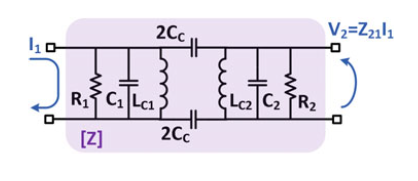
\includegraphics{figures/capicitively-coupled-resonator.PNG}
    \caption{Capacitively coupled resonators schematic \cite{5G-and-E-band}.}
    \label{fig:capacitively-coupled-resonators}
\end{figure}

\begin{equation}
    Y_{11}=Y_{22}=\frac{1}{R}+\frac{1}{sL_C}+s\left (C+C_C\right)=\frac{1}{R}\left [1+Q\left (\frac{s}{\omega_0}+\frac{\omega_0}{s}\right)\right]
\end{equation}
\begin{equation}
    Y_{21}=Y_{12}=-sC_C=-\frac{sk_CQ}{\omega_0 R}
\end{equation}

Where
\begin{align}
    \omega_0&=\frac{1}{\sqrt{L_C\left (C+C_C\right)}}\\
    Q&=\frac{R}{\omega_0 L_C}=\omega_0R\left (C+C_C\right) \label{Q_increase}\\
    k_c&=\frac{C_C}{C+C_C}
\end{align}

The two-port network's transimpedance can be determined as \cite{5710437,microwave-engineering}
\begin{equation}
    \begin{split}
        Z_{21}&=\frac{-Y_[21]}{Y_{11}Y_{22}-Y_{12}Y_{21}}\\ &=\frac{s^3k_CQ\omega_0R}{\left [Q\left (1+k_C\right )s^2+s\omega_0+Q\omega_0^2\right]\left [Q\left (1-k_C\right )s^2+s\omega_0+Q\omega_0^2\right]}
    \end{split}
\end{equation}

Assuming high quality factor, the two complex poles of $Z_{21}$ can be calculated as
\begin{align}
    \omega_L=\frac{1}{\sqrt{L_C\left (C+2C_C\right )}}\\
    \omega_H=\frac{1}{\sqrt{L_CC}}
\end{align}

A higher $C_C$ provides for a wider band-pass bandwidth at the expense of the network's quality factor Equation \eqref{Q_increase} and in-band ripple.

\subsection{Inductively Coupled Resonators}
An inductor $L_c$ can be used to couple two RLC tanks, resulting in a filter with a schematic shown in Figure \ref{fig:inductively-coupled-resonators} \cite{WidebandReceiver,6942051} expressed as.

\begin{figure}[h]
    \centering
    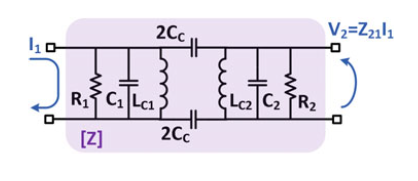
\includegraphics{figures/capicitively-coupled-resonator.PNG}
    \caption{Inductively coupled
resonators schematic \cite{5G-and-E-band}.}
    \label{fig:inductively-coupled-resonators}
\end{figure}

\begin{equation}
    Y_{11}=Y_{22}=\frac{1}{R}+\frac{L_{LC}+L_L}{s L_L L_{LC}}+sC=\frac{1}{R}\left [1+Q\left (\frac{s}{\omega_o}+\frac{\omega_0}{s}\right )\right]
\end{equation}

\begin{equation}
    Y_{21}=Y_{12}=-\frac{1}{sL_{LC}}=-\frac{\omega_0k_LQ}{sR}
\end{equation}
where
\begin{align}
    &\omega_0=\frac{1}{\sqrt{\frac{L_L L_{LC}}{L_L+L_{LC}}}}\\
    &Q=\frac{R\left(L_L+L_{LC}\right )}{\omega_0 L_L L_{LC}}=\omega_0 RC\\
    &k_L=\frac{L_L}{L_{LC}+L_L}
\end{align}

The two-port network's transimpedance value can be calculated using
\begin{equation}
    Z_{21}=\frac{\omega_0^3k_LQRs}{\left [Qs^2+s\omega_0+Q\left (1+k_L\right )\omega_0^2\right ]\left [Qs^2+s\omega_0+Q\left (1-k_L\right )\omega_0^2\right]}
\end{equation}

If we assume a high quality factor, we can determine the two complex poles of $Z_{21}$ as follows:
\begin{align}
    \omega_L&=\frac{1}{L_LC}\\
    \omega_H&=\frac{1}{\frac{L_L L_{LC}}{2L_L+L_{LC}C}}
\end{align}

Opting for a smaller $L_{LC}$ value can result in a wider band-pass bandwidth, but it also leads to higher in-band ripple.

\subsection{Magnetically Coupled Resonators}
A transformer can be realized by using two magnetically coupled inductors \cite{868049}. Figure \ref{fig:transformer} shows the resulting schematic of the 2-port network, along with three equivalent models.

\begin{figure}[h]
    \centering
    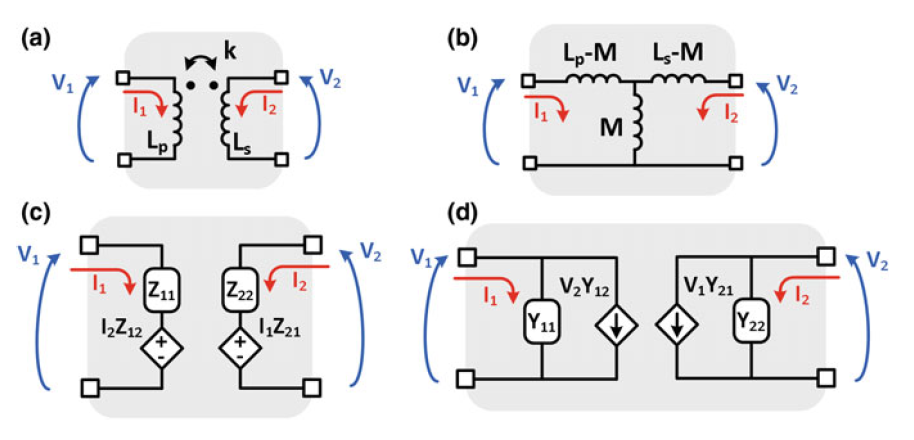
\includegraphics[width=\textwidth]{figures/transformer.PNG}
    \caption{Transformer (a) schematic symbol, (b) equivalent T-section model, (c) Z-parameter and d Y-parameter 2-port models \cite{5G-and-E-band}.}
    \label{fig:transformer}
\end{figure}

The Y-parameter matrix can be defined when the losses are represented as ideal resistors in parallel with ideal inductors.
\begin{equation}
\begin{bmatrix}
I_1 \\ I_2
\end{bmatrix} = 
\begin{bmatrix}
Y_{11} & Y_{12} \\
Y_{21} & Y_{22}
\end{bmatrix}
\begin{bmatrix}
V_1 \\ V_2
\end{bmatrix}=
\begin{bmatrix}
\frac{1}{R_{P,p}}+\frac{1}{j\omega L_p\left (1-k^2\right )} & \frac{k}{j\omega \sqrt{\left (L_p L_s\right )}\left (1-k^2\right)} \\
\frac{k}{j\omega \sqrt{\left (L_p L_s\right )}\left (1-k^2\right)} & \frac{1}{R_{P,s}}+\frac{1}{j\omega L_s\left (1-k^2\right )}
\end{bmatrix}
\begin{bmatrix}
V_1 \\ V_2
\end{bmatrix}
\label{transformer-Y-parameter}
\end{equation}

The parallel resistor and self-inductance of the primary and secondary windings are denoted as $R_{P,p}$, $L_p$, $R_{P,s}$, and $L_s$, respectively.

The practical limitations of on-chip transformers are similar to those of on-chip inductors. However, there are two main differences. Firstly, transformers exhibit a lower self-resonant frequency due to the presence of parasitic inter-winding capacitance. Secondly, the magnetic field between the two coils is more confined, thereby reducing the negative impact of dummies when compared to inductors \cite{6578194,6858393}.

A transformer can be used to couple two RLC tanks together, as shown in Figure \ref{fig:magnetically-coupled-resonators} \cite{7418056}. Assuming $R_1 = R_2 = R$, $C_1 = C_2 = C$, and $L_{M1} = L_{M2} = L_M$, it is easy to obtain the admittance parameters of this two-port network by using the Y-parameter model of the transformer given in equation \eqref{transformer-Y-parameter}.

\begin{figure}[h]
    \centering
    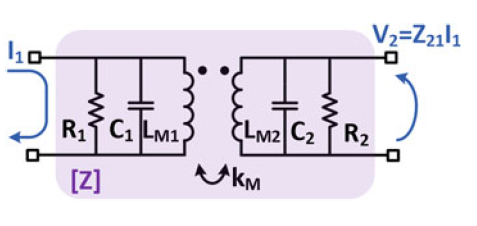
\includegraphics{figures/magnetically-coupled-resonators.PNG}
    \caption{Magnetically coupled
resonators schematic \cite{5G-and-E-band}.}
    \label{fig:magnetically-coupled-resonators}
\end{figure}

\begin{equation}
    Y_{11}=Y_{22}=\frac{1}{R}+\frac{1}{sL_M\left (1-k_M^2\right )}+sC=\frac{1}{R}\left[1+Q\left (\frac{s}{\omega_0}+\frac{\omega_0}{s}\right )\right]
\end{equation}
\begin{equation}
    Y_{21}=Y_{12}=\frac{k_M}{sL_M\left (1-k_M^2\right )}=\frac{k_M\omega_0Q}{sR}
\end{equation}
where
\begin{align}
    &\omega_0=\frac{1}{\sqrt{L_M\left (1-k_M^2\right )}C}\\
    &Q=\frac{R}{\omega_0L_M\left (1-k_M^2\right )}=\omega_0RC \label{magnetic_Q}
\end{align}

The transimpedance value of the two-port network can be determined by
\begin{equation}
    Z_{21}=\frac{-\omega_0^3k_MQRs}{\left [Qs^2+s\omega_0+Q\left (1+k_M\right )\omega_0^2\right ]\left [Qs^2+s\omega_0+Q\left (1-k_M\right )\omega_0^2\right]}
\end{equation}

If we assume a high quality factor, we can determine the two complex poles of $Z_{21}$ as follows:
\begin{align}
    &\omega_L=\frac{1}{\sqrt{L_M\left(1+\left|k_M\right|\right)C}}\\
    &\omega_H-\frac{1}{\sqrt{L_M\left(1-\left|k_M\right|\right)C}}
\end{align}

Increasing the magnetic coupling coefficient k leads to a wider band-pass bandwidth of the filter. However, it comes at the cost of increased in-band ripple and Q-factor of the filter as shown in equation \ref{magnetic_Q}.

\section{Wideband Matching Network Design using ADS}
 \begin{figure}
     \centering
     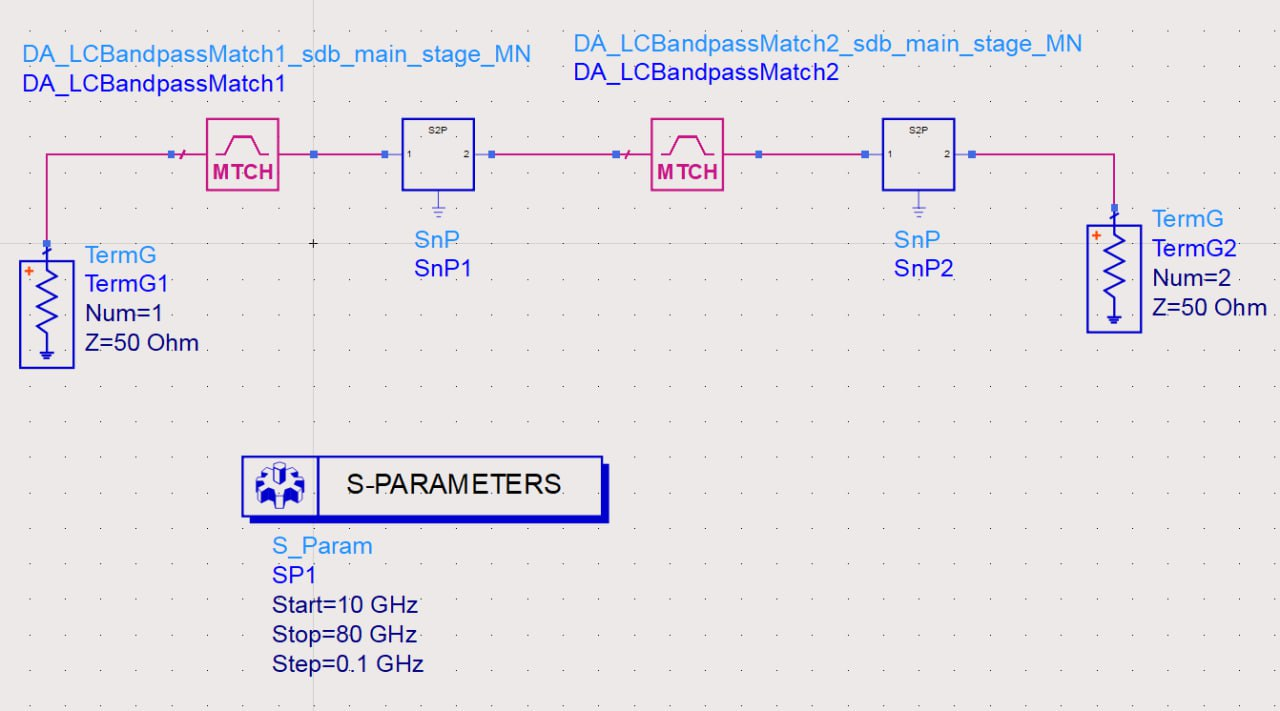
\includegraphics[scale=0.5]{figures/matching-ADS.jpeg}
     \caption{Wide-band matching network design environment using ADS.}
     \label{fig:matching-network-ads}
 \end{figure}
 
\subsection{Input Matching Network Design}
 The proposed CMOS power amplifier's input matching network is made to match the impedance of the input signal source to the amplifier's impedance for effective power transfer. It often includes passive parts like transmission lines, inductors, and capacitors.

The intended performance and operating frequency of the power amplifier determine the precise architecture of the input matching network. L-section matching, T-section matching, $\Pi$-section matching, and distributed matching are examples of common matching topologies.

The proposed input matching network's goals are to reduce input signal reflection, increase power transmission, and provide impedance transformation so that the source impedance can be matched to the amplifier's input impedance. This makes sure the power amplifier functions as efficiently as possible and outputs the most power possible.

By using ADS software, we have selected appropriate component values and dimensions based on the desired frequency response, impedance transformation ratio, and power handling capabilities.
 \begin{figure}[h]
     \centering
     \begin{circuitikz}[american, scale=1, thick]
    \draw (0,0) node[left]{$IN$} to[short, o-] ++(1,0) coordinate(A)
    to[L, l=$L_1$] ++(3,0) coordinate(B)
    to[L, l=$L_3$] ++(2,0) to[short, -o] ++(0.5,0) node[right]{$OUT$};
    \draw (A) to[C, l=$C$, *-] ++(0,-2) node[ground]{};
    \draw (B) to[L, l=$L_2$, *-] ++(0,-2) node[ground]{};
    \end{circuitikz}
     \caption{Input matching network of proposed CMOS power amplifier.}
     \label{fig:input-matching-network}
 \end{figure}
 \begin{table}[h]
  \centering
  \caption{Component value of input matching network, Figure \ref{fig:input-matching-network}.}
  \label{tab:component-value-input-matching-network}
  \begin{tabular}{@{}cccc@{}}
    \toprule
    \textbf{$C$} & \textbf{$L_1$} & \textbf{$L_2$} & \textbf{$L_3$} \\
    \midrule
    \SI{355.13}{\femto\farad} & \SI{53.745}{\pico\henry} & \SI{24.23}{\pico\henry} & \SI{68.55}{\pico\henry}  \\
    \bottomrule
  \end{tabular}
\end{table}

\subsection{Interstage Matching Network Design}
In multi-stage amplifier designs, interstage matching networks are employed to maintain impedance matching and guarantee effective power transmission between stages. In order to match the input impedance of one stage to the output impedance of the following stage, these networks are positioned between successive amplifier stages, Figure \ref{fig:double-stage-power-amplifier}.
\begin{figure}[h]
    \centering
    \begin{circuitikz}[american, scale=1, thick]
    \draw (0,0) node[left]{$IN$}
    to[C, l=$C_1$, o-] ++(2,0) -- ++(.5,0) coordinate(A)-- ++(0.5,0)
    to[L, l=$L_1$] ++(2,0) -- ++(0.5,0) coordinate(B)
    to[short] ++(2,0) coordinate(C)
    to[L, l=$L_3$, -o] ++(2,0)node[right]{$OUT$};
    \draw (A) to[C, l=$C_2$, *-] ++(0,-2)node[ground]{};
    \draw (B) to[L, l=$L_2$, *-] ++(0,-2)node[ground]{};
    \draw (C) to[C, l=$C_3$, *-] ++(0,-2) node[ground]{};
\end{circuitikz}
    \caption{Interstage matching network design using ADS.}
    \label{fig:interstage-matching-network}
\end{figure}
\begin{table}[h]
  \centering
  \caption{Component value of interstage matching network.}
  \label{tab:component-value-interstage-matching-network}
  \begin{tabular}{@{}cccccc@{}}
    \toprule
    \textbf{$C_1$} & \textbf{$C_2$} & \textbf{$L_1$} & \textbf{$L_2$} & \textbf{$C_3$} &  \textbf{$L_3$}\\
    \midrule
    \SI{56.28}{\femto\farad} & \SI{225.8}{\femto\farad} & \SI{110.143}{\pico\henry} & \SI{3.72}{\pico\henry} & \SI{7.696}{\pico\farad} & \SI{83.94}{\pico\henry} \\
    \bottomrule
  \end{tabular}
\end{table}
\section{Dual Band PA Circuit}
\subsection{Single Stage PA}
The cascode amplifier has an extremely high input resistance and a voltage gain that can reach $A^2$ when the CS and CG variants are combined. A single stage power amplifier (PA) designed by the superimposed staggered technique shown in Figure \ref{fig:single-stage-power-amplifier}.
\begin{figure}[H]
    \centering
   \begin{circuitikz}[american, scale=0.7, thick]
      \draw (0,0) node[left]{$IN$} to[short, o-] ++(0.5,0) 
      to[C, l=$C_2$] ++(2,0) -- ++(1,0) coordinate(E) -- ++(1.5,0) node[nigfete, anchor=G](mos1){$M_1$}
        (mos1.S) node[ground]{}
        (mos1.D) to[short] ++(0,3) node[nigfete](mos2){$M_2$}
        (mos2.D) to[short] ++(0,1) to[L, l=$L_4$] ++(0,2) node[vcc]{$V_{DD1}$}
        (mos2.G) -- ++(-1.5,0) coordinate(F) -- ++(-1,0)
        to[C, l=$C_3$] ++(-2,0) 
        to[short] ++(-0.5,0) node[ground]{};
        \draw (E) to[R, l=$R_1$, *-] ++(0,2) node[vcc]{$V_{G1-CS}$};
        \draw (F) to[R, l=$R_2$, *-] ++(0,2) node[vcc]{$V_{G1-CG}$};
        \draw (mos2.D) to[short, *-o] ++(1,0) node[right]{$OUT$};
  \end{circuitikz}
    \caption{Single stage power amplifier without matching network..}
    \label{fig:single-stage-power-amplifier}
  \end{figure}
\subsubsection{Operating Point Analysis}
For effective and linear amplification in a power amplifier, the transistor should be operating in the saturation area. The transistor is biased in the saturation region when the drain-source voltage ($V_{DS}$) is high enough to maintain a fully open channel and the gate-source voltage ($V_{GS}$) is greater than the threshold voltage ($V_{th}$).

The transistor can reach its maximum current carrying capacity and low output impedance by operating in the saturation region. The power amplifier circuit benefits from high gain, high output power, and good linearity as a result.

By choosing appropriate DC operating points, such as the drain current ($I_D$) and the drain-source voltage ($V_{DS}$) levels, the transistor must be properly biased in order to function correctly in the saturation area. Depending on the specific needs of the power amplifier circuit, such as the intended output power, linearity, and efficiency, the biasing conditions may change.
 \begin{figure}[H]
  \centering
  \begin{subfigure}{0.49\textwidth}
    \centering
    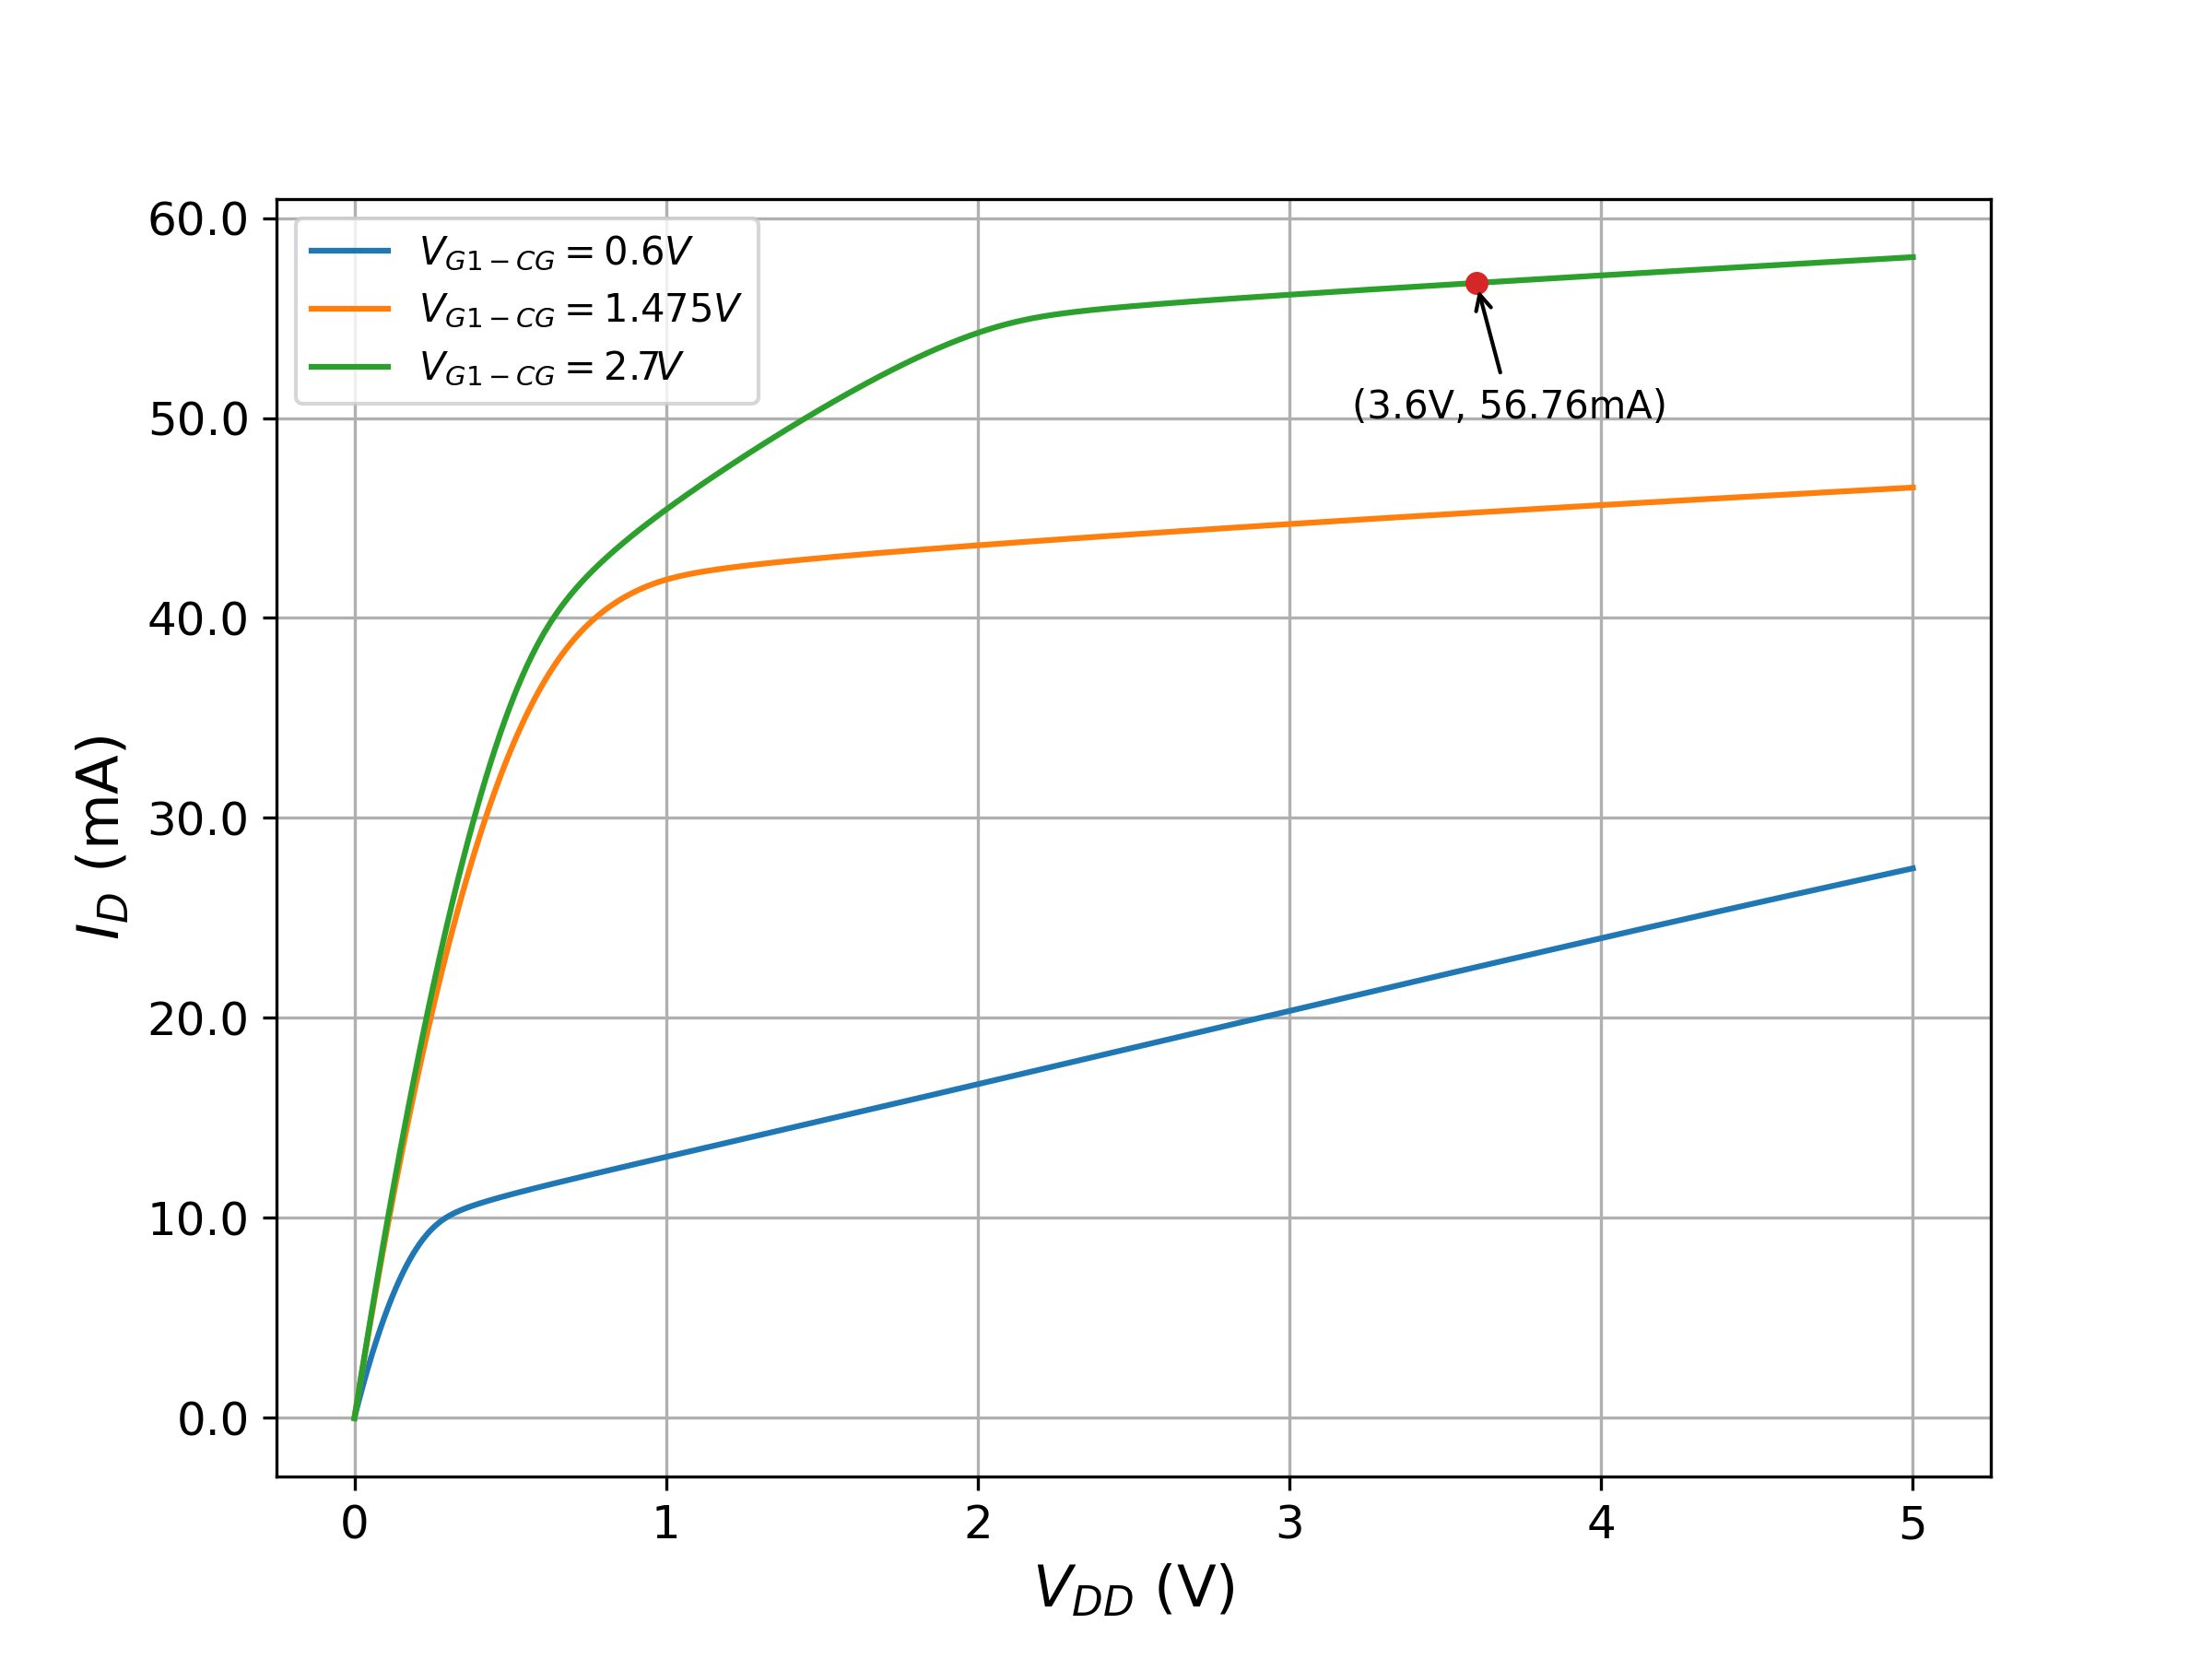
\includegraphics[width=\linewidth]{figures/id-vs-vds-parametric-gs2.png}
    \caption{}
    \label{fig:id-vs-vdd-parametric-gs2}
  \end{subfigure}
  \hfill
  \begin{subfigure}{0.49\textwidth}
    \centering
    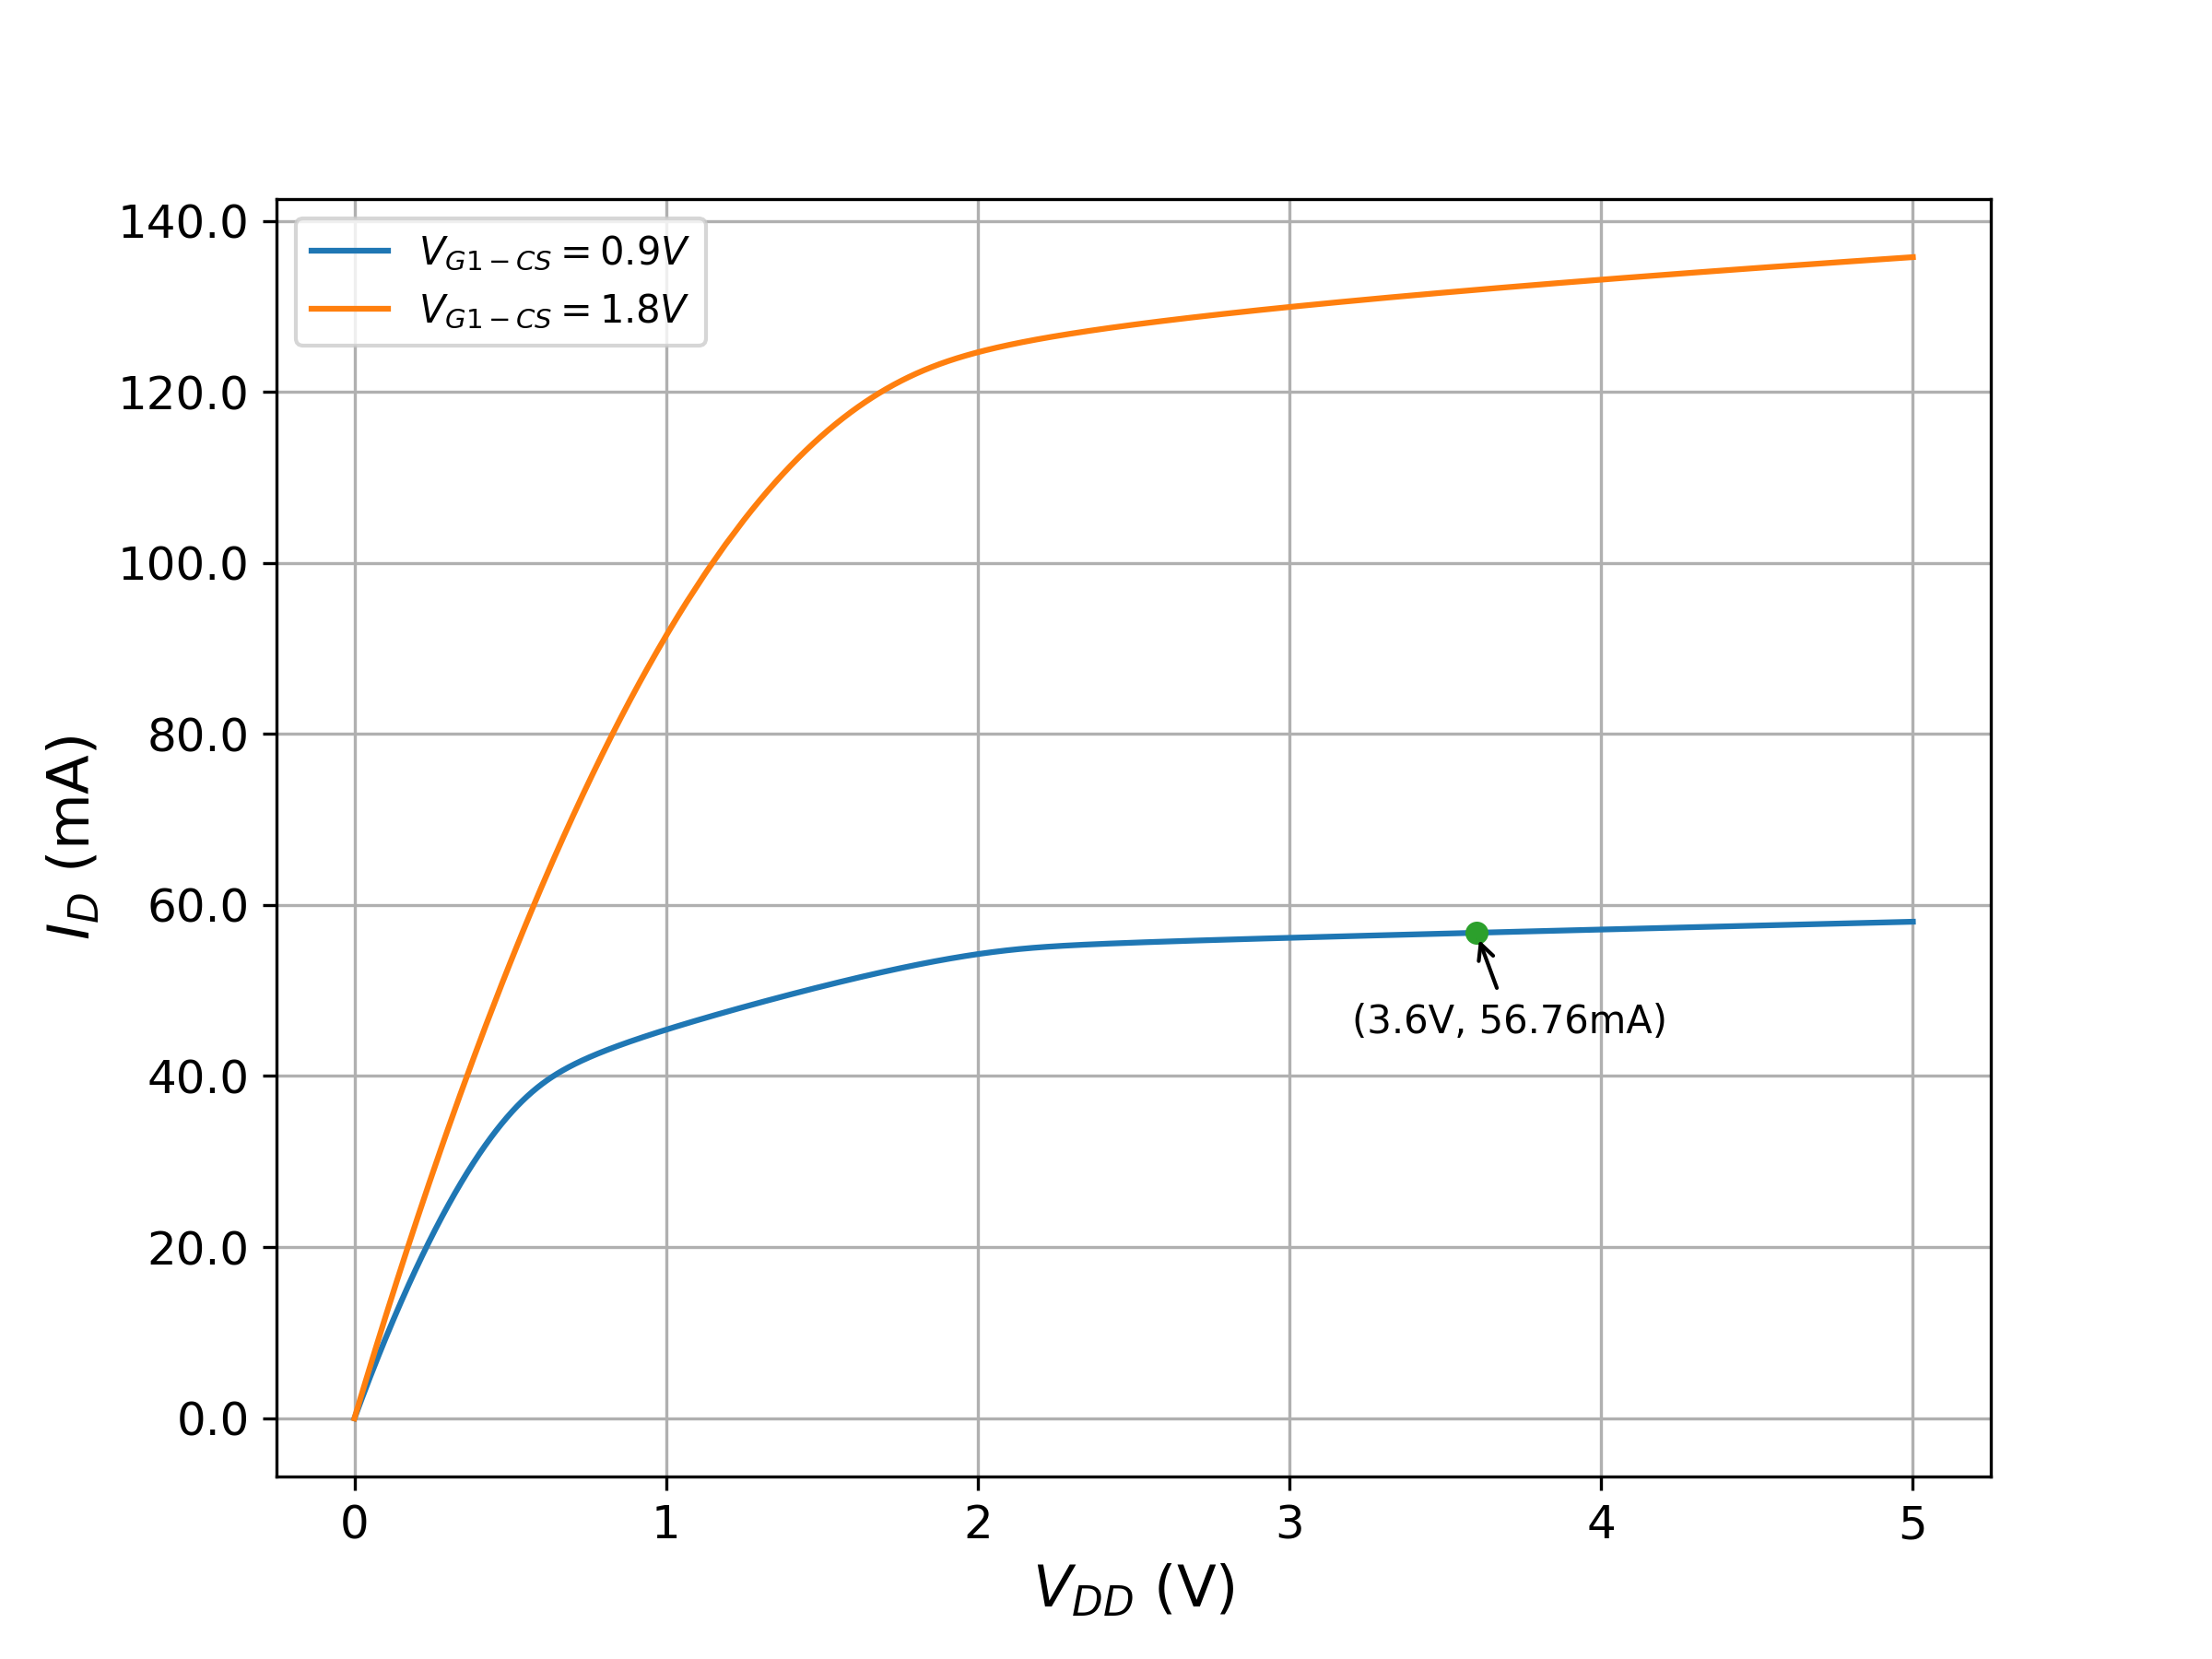
\includegraphics[width=\linewidth]{figures/id-vs-vds-parametric-gs1.png}
    \caption{}
     \label{fig:id-vs-vdd-parametric-gs1}
  \end{subfigure}
  \caption{(a) Drain current ($I_D$) vs $V_{DD}$ when changing $V_{G1-CG}$ (b)  Drain current ($I_D$) vs $V_{DD}$ when changing $V_{G1-CS}$.}
  \label{fig:id-vs-vdd-gs1-gs2}
\end{figure}

To select the operating point at the saturation region from Figure \ref{fig:id-vs-vdd-parametric-gs2}, select supply voltage $V_{DD}$ is 3.6V, $V_{G1-CG}$ is 2.7V, and saturate current 56.76 mA. To maintain a saturation current of 56.76 mA, the $V_{G1-CS}$ should be 0.9V shown in Figure \ref{fig:id-vs-vdd-parametric-gs1}.
\begin{table}[H]
  \centering
  \caption{Component value of first stage PA, Figure \ref{fig:single-stage-power-amplifier}.}
  \label{tab:component-value-of-first-stage}
  \begin{tabular}{@{}ccccc@{}}
  %\begin{tabular}{\textwidth}{@{}XXXXXXXXXX@{}}
    \toprule
    \textbf{$C_2$} & \textbf{$C_3$} & \textbf{$R_1$} & \textbf{$R_2$} & \textbf{$L_4$} \\
    \midrule
    \SI{810}{\femto\farad} & \SI{860}{\femto\farad} & \SI{11}{\kilo\ohm} & \SI{11}{\kilo\ohm} & \SI{242}{\pico\henry} \\
    \midrule
    \textbf{$V_{G1-CG}$} & \textbf{$V_{G1-CS}$} & \textbf{$M1_{W/L}$} & \textbf{$M2_{W/L}$} & \textbf{$V_{DD1}$}\\
    \midrule
     \SI{2.7}{\volt} & \SI{0.9}{\volt} & \SI{160}{\um}/\SI{180}{\nm} & \SI{160}{\um}/\SI{180}{\nm} & \SI{3.6}{\volt}\\
    \bottomrule
  \end{tabular}
\end{table}

\newpage
\subsection{Two Stage PA}
In order to provide more gain and bandwidth, a second stage is connected to the first stage.
\begin{figure}[H]
    \centering
   \begin{circuitikz}[american, scale=0.7, thick]
      \draw (0,0) node[left]{$IN$} to[short, o-] ++(0.5,0) 
      to[C, l=$C_2$] ++(2,0) -- ++(1,0) coordinate(E) -- ++(1.5,0) node[nigfete, anchor=G](mos1){$M_1$}
        (mos1.S) node[ground]{}
        (mos1.D) to[short] ++(0,3) node[nigfete](mos2){$M_2$}
        (mos2.D) to[short] ++(0,1) to[L, l=$L_4$] ++(0,2) node[vcc]{$V_{DD1}$}
        (mos2.G) -- ++(-1.5,0) coordinate(F) -- ++(-1,0)
        to[C, l=$C_3$] ++(-2,0) 
        to[short] ++(-0.5,0) node[ground]{};
        \draw (E) to[R, l=$R_1$, *-] ++(0,2) node[vcc]{$V_{G1-CS}$};
        \draw (F) to[R, l=$R_2$, *-] ++(0,2) node[vcc]{$V_{G1-CG}$};
        \draw (mos2.D) to[short, *-] ++(1,0) coordinate(H);

        \draw (H) to[short] ++(1,0) 
      to[C, l=$C_2$] ++(2,0) -- ++(1,0) coordinate(E) -- ++(1.5,0) node[nigfete, anchor=G](mos3){$M_1$}
        (mos3.S) node[ground]{}
        (mos3.D) to[short] ++(0,3) node[nigfete](mos4){$M_2$}
        (mos4.D) to[short] ++(0,1) to[L, l=$L_4$] ++(0,2) node[vcc]{$V_{DD1}$}
        (mos4.G) -- ++(-1.5,0) coordinate(F) -- ++(-1,0)
        to[C, l=$C_3$] ++(-2,0) 
        to[short] ++(-0.5,0) node[ground]{};
        \draw (E) to[R, l=$R_1$, *-] ++(0,2) node[vcc]{$V_{G1-CS}$};
        \draw (F) to[R, l=$R_2$, *-] ++(0,2) node[vcc]{$V_{G1-CG}$};
        \draw (mos4.D) to[short, *-o] ++(0.5,0) node[right]{$OUT$};
  \end{circuitikz}
    \caption{Two stage power amplifier without matching network..}
    \label{fig:double-stage-power-amplifier}
  \end{figure}

\subsection{Two Stage PA With Matching Network}
An input-matching network is designed to match thetransistor’s impedance with the source impedance. An interstage matching network is also designed tomatch the first and second stages’ impedances.
  \begin{figure}[H]
    \centering
   \begin{circuitikz}[american,scale=0.8, thick]
        \draw (0,0) node[left]{$IN$} to[short, o-] ++(1,0) coordinate(A)-- ++(0.5,0)
        to[L, l=$L_1$] ++(2,0)-- ++(0.5,0) coordinate(B) -- ++(0.5,0)
        to[L, l=$L_3$] ++(2,0) to[short] ++(0.5,0) coordinate(C);
        \draw (A) to[C, l=$C_1$, *-] ++(0,-2) node[ground]{};
        \draw (B) to[L, l=$L_2$, *-] ++(0,-2) node[ground]{};
        
        \draw (C) to[C, l=$C_2$] ++(2,0) -- ++(1,0) coordinate(E) -- ++(1.5,0) node[nigfete, anchor=G](mos1){$M_1$}
        (mos1.S) node[ground]{}
        (mos1.D) to[short] ++(0,3) node[nigfete](mos2){$M_2$}
        (mos2.D) to[short] ++(0,1) to[L, l=$L_4$] ++(0,2) node[vcc]{$V_{DD1}$}
        (mos2.G) -- ++(-1.5,0) coordinate(F) -- ++(-1,0)
        to[C, l=$C_3$] ++(-2,0) 
        to[short] ++(-0.5,0) node[ground]{};
        \draw (E) to[R, l=$R_1$, *-] ++(0,2) node[vcc]{$V_{G1-CS}$};
        \draw (F) to[R, l=$R_2$, *-] ++(0,2) node[vcc]{$V_{G1-CG}$};
        \draw (mos2.D) to[short] ++(1,0) coordinate(H);
    \end{circuitikz}
    \caption{First stage of proposed power amplifier with input matching network.}
    \label{fig:first-stage-with-input-match}
  \end{figure}

\begin{figure}[H]
    \centering
    \begin{circuitikz}[american, scale=0.8, thick]
        \draw (0,0)
        to[C, l=$C_4$] ++(2,0) -- ++(.5,0) coordinate(A)-- ++(0.5,0)
        to[L, l=$L_5$] ++(2,0) -- ++(1,0) coordinate(B)
        to[short] ++(2,0) coordinate(C) -- ++(1,0)
        to[L, l=$L_7$] ++(2,0) coordinate(end_inters);
        \draw (A) to[C, l=$C_5$, *-] ++(0,-2)node[ground]{};
        \draw (B) to[L, l=$L_6$, *-] ++(0,-2)node[ground]{};
        \draw (C) to[C, l=$C_6$, *-] ++(0,-2) node[ground]{};

        \draw (end_inters) to[short] ++(0.5,0)
      to[C, l=$C_2$] ++(2,0) -- ++(1,0) coordinate(E) -- ++(1.5,0) node[nigfete, anchor=G](mos3){$M_1$}
        (mos3.S) node[ground]{}
        (mos3.D) to[short] ++(0,3) node[nigfete](mos4){$M_2$}
        (mos4.D) to[short] ++(0,1) to[L, l=$L_4$] ++(0,2) node[vcc]{$V_{DD1}$}
        (mos4.G) -- ++(-1.5,0) coordinate(F) -- ++(-1,0)
        to[C, l=$C_3$] ++(-2,0) 
        to[short] ++(-0.5,0) node[ground]{};
        \draw (E) to[R, l=$R_1$, *-] ++(0,2) node[vcc]{$V_{G1-CS}$};
        \draw (F) to[R, l=$R_2$, *-] ++(0,2) node[vcc]{$V_{G1-CG}$};
        \draw (mos4.D) to[short, *-o] ++(0.5,0) node[right]{$OUT$};
    \end{circuitikz}
    \caption{Second stage of proposed PA with interstage matching network}
    \label{fig:second-stage-with-matching-network}
\end{figure}

\begin{figure}[H]
    \centering
     \resizebox{\textwidth}{!}{
   \begin{circuitikz}[american,scale=1, thick]
        \draw (0,0) node[left]{$IN$} to[short, o-] ++(1,0) coordinate(A)-- ++(0.5,0)
        to[L, l=$L_1$] ++(2,0)-- ++(0.5,0) coordinate(B) -- ++(0.5,0)
        to[L, l=$L_3$] ++(2,0) to[short] ++(0.5,0) coordinate(C);
        \draw (A) to[C, l=$C_1$, *-] ++(0,-2) node[ground]{};
        \draw (B) to[L, l=$L_2$, *-] ++(0,-2) node[ground]{};
        
        \draw (C) to[C, l=$C_2$] ++(2,0) -- ++(1,0) coordinate(E) -- ++(1.5,0) node[nigfete, anchor=G](mos1){$M_1$}
        (mos1.S) node[ground]{}
        (mos1.D) to[short] ++(0,3) node[nigfete](mos2){$M_2$}
        (mos2.D) to[short] ++(0,1) to[L, l=$L_4$] ++(0,2) node[vcc]{$V_{DD1}$}
        (mos2.G) -- ++(-1.5,0) coordinate(F) -- ++(-1,0)
        to[C, l=$C_3$] ++(-2,0) 
        to[short] ++(-0.5,0) node[ground]{};
        \draw (E) to[R, l=$R_1$, *-] ++(0,2) node[vcc]{$V_{G1-CS}$};
        \draw (F) to[R, l=$R_2$, *-] ++(0,2) node[vcc]{$V_{G1-CG}$};
        \draw (mos2.D) to[short, *-] ++(1,0) coordinate(H);


        \draw (H)
        to[C, l=$C_4$] ++(2,0) -- ++(.5,0) coordinate(A)-- ++(0.5,0)
        to[L, l=$L_5$] ++(2,0) -- ++(1,0) coordinate(B)
        to[short] ++(2,0) coordinate(C) -- ++(1,0)
        to[L, l=$L_7$] ++(2,0) coordinate(end_inters);
        \draw (A) to[C, l=$C_5$, *-] ++(0,-2)node[ground]{};
        \draw (B) to[L, l=$L_6$, *-] ++(0,-2)node[ground]{};
        \draw (C) to[C, l=$C_6$, *-] ++(0,-2) node[ground]{};

        \draw (end_inters) to[short] ++(0.5,0)
      to[C, l=$C_2$] ++(2,0) -- ++(1,0) coordinate(E) -- ++(1.5,0) node[nigfete, anchor=G](mos3){$M_1$}
        (mos3.S) node[ground]{}
        (mos3.D) to[short] ++(0,3) node[nigfete](mos4){$M_2$}
        (mos4.D) to[short] ++(0,1) to[L, l=$L_4$] ++(0,2) node[vcc]{$V_{DD1}$}
        (mos4.G) -- ++(-1.5,0) coordinate(F) -- ++(-1,0)
        to[C, l=$C_3$] ++(-2,0) 
        to[short] ++(-0.5,0) node[ground]{};
        \draw (E) to[R, l=$R_1$, *-] ++(0,2) node[vcc]{$V_{G1-CS}$};
        \draw (F) to[R, l=$R_2$, *-] ++(0,2) node[vcc]{$V_{G1-CG}$};
        \draw (mos4.D) to[short, *-o] ++(0.5,0) node[right]{$OUT$};
    \end{circuitikz}
    }
    \caption{With input and an interstage matching network, a two-stage power amplifier.}
    \label{fig:two-stage-with-input-interstage-matching}
  \end{figure}
\chapter{RESULT \& ANALYSIS}
\section{Result}
 %The $S$ parameter simulation of single stage power amplifier(Figure \ref{fig:single-stage-power-amplifier}) is shown below
 \begin{figure}[H]
  \centering
  \begin{subfigure}{0.49\textwidth}
    \centering
    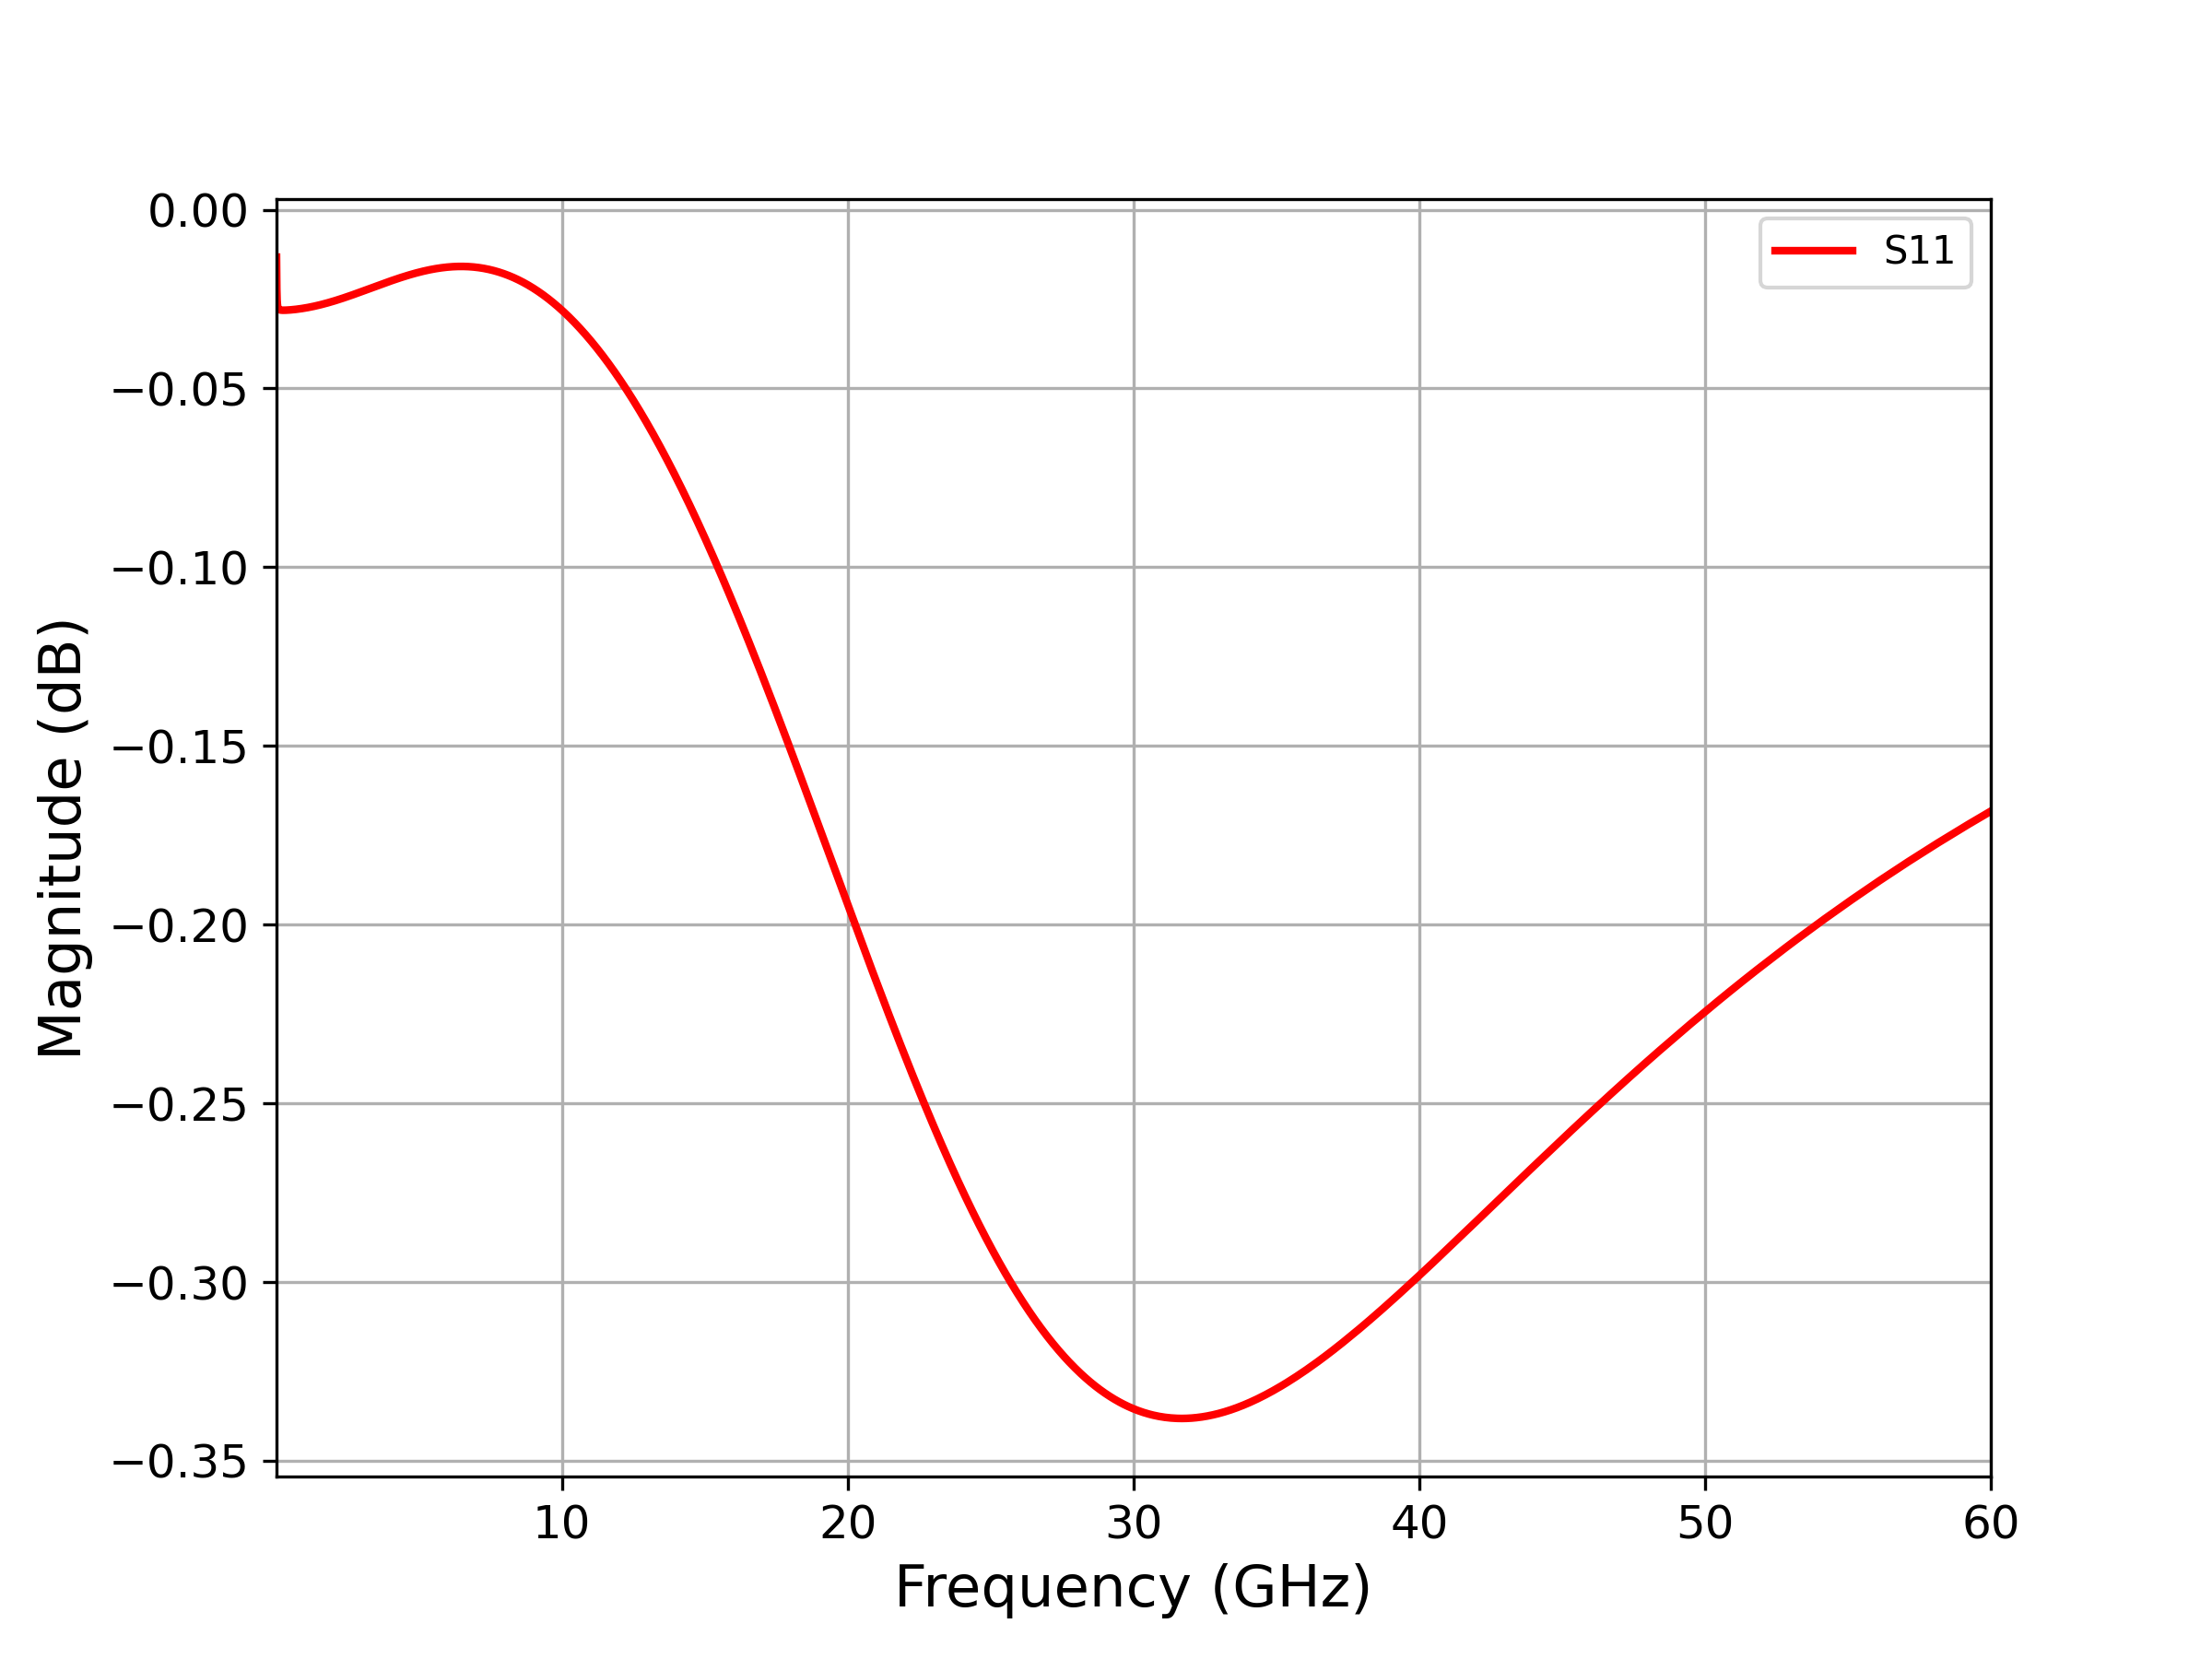
\includegraphics[width=\linewidth]{figures/single_stage_s11.png}
    \caption{}
    \label{fig:single-stage-without-cadence-s11}
  \end{subfigure}
  \hfill
  \begin{subfigure}{0.49\textwidth}
    \centering
    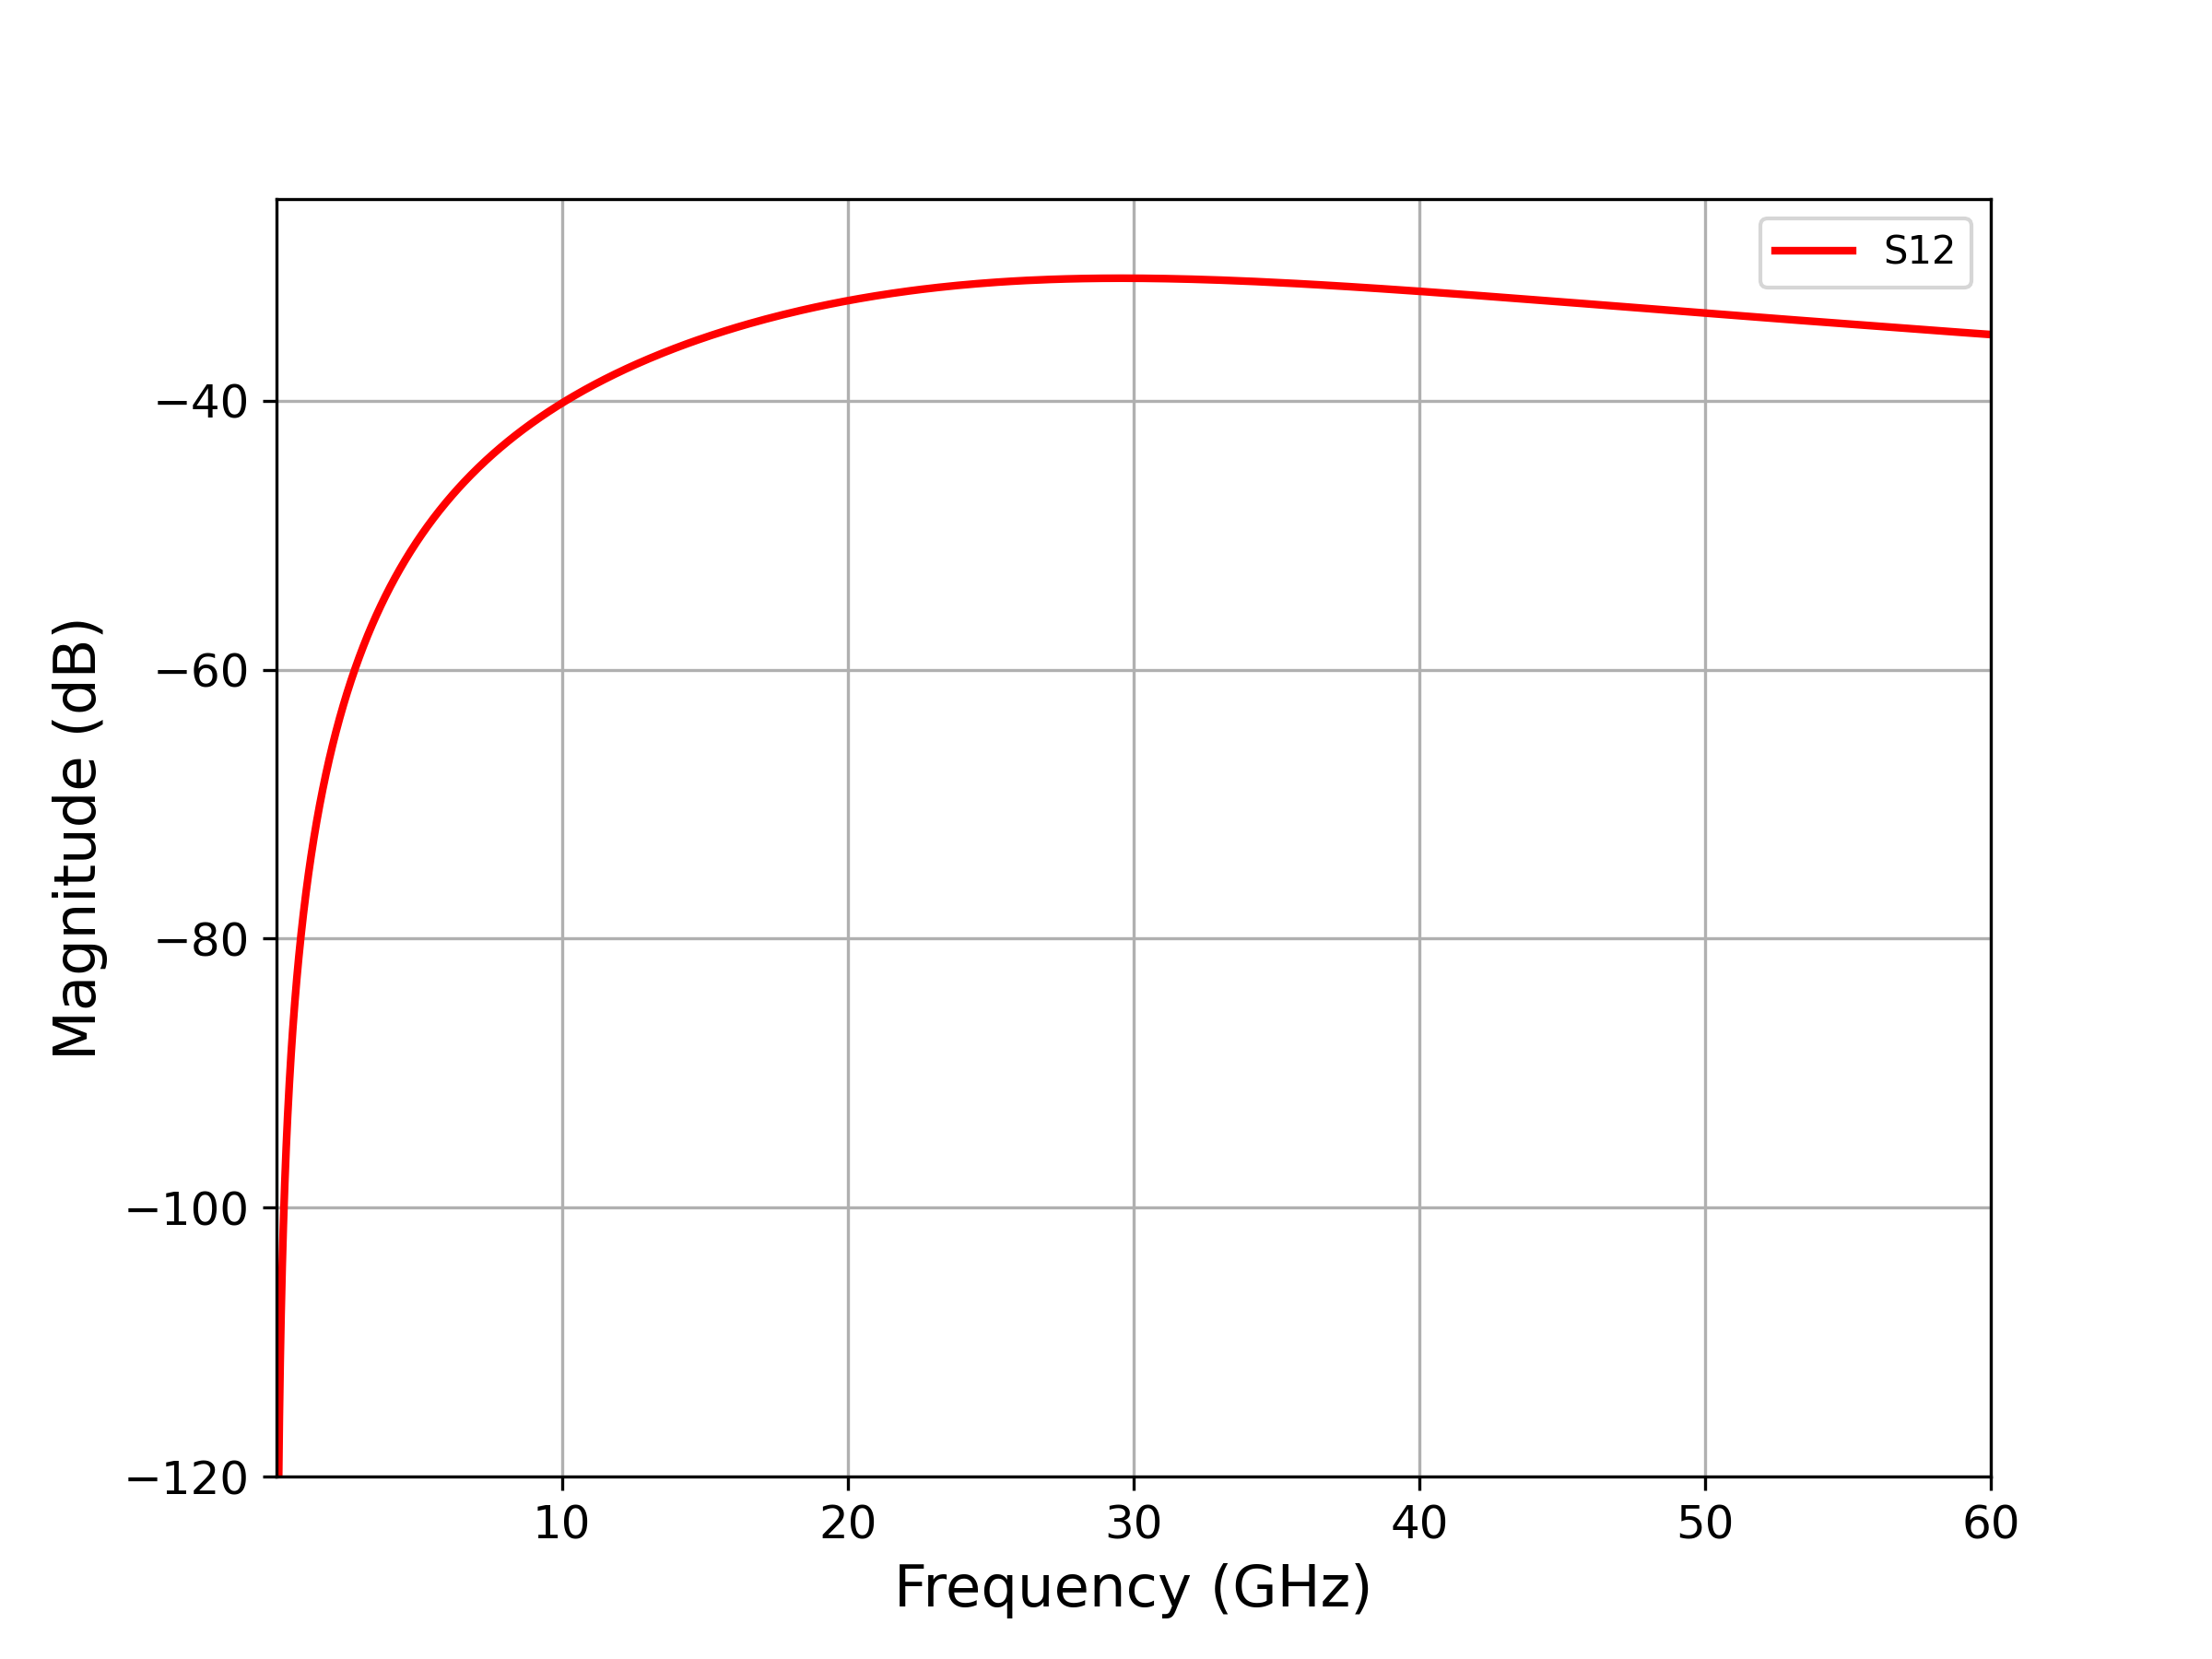
\includegraphics[width=\linewidth]{figures/single_stage_s12.png}
    \caption{}
     \label{fig:single-stage-without-cadence-s12}
  \end{subfigure}
  \caption{(a) $S_{11}$ parameter of a single-stage power amplifier (shown in Figure \ref{fig:single-stage-power-amplifier}) without matching network. (b) $S_{12}$ parameter of a single-stage power amplifier (shown in Figure \ref{fig:single-stage-power-amplifier}) without matching network.}
  \label{fig:single-stage-without-cadence-s11-s12}
\end{figure}

The value of $S_{11}$ of a single-stage power amplifier is -0.17 dB at frequency 18 GHz, which indicates poor input matching. This means a significant portion of the power is being reflected back rather than absorbed by the amplifier, leading to inefficiency. The Return Loss ($S_{12}$) parameter represents the power reflected back from Port 2 (the incident signal) to Port 1 (the reflected signal) in a two-port network. The value of $S_{12}$ a single-stage power amplifier is less than -30 dB through the BW.
% \begin{figure}[H]
%     \centering
%     \resizebox{0.8\textwidth}{!}{
%     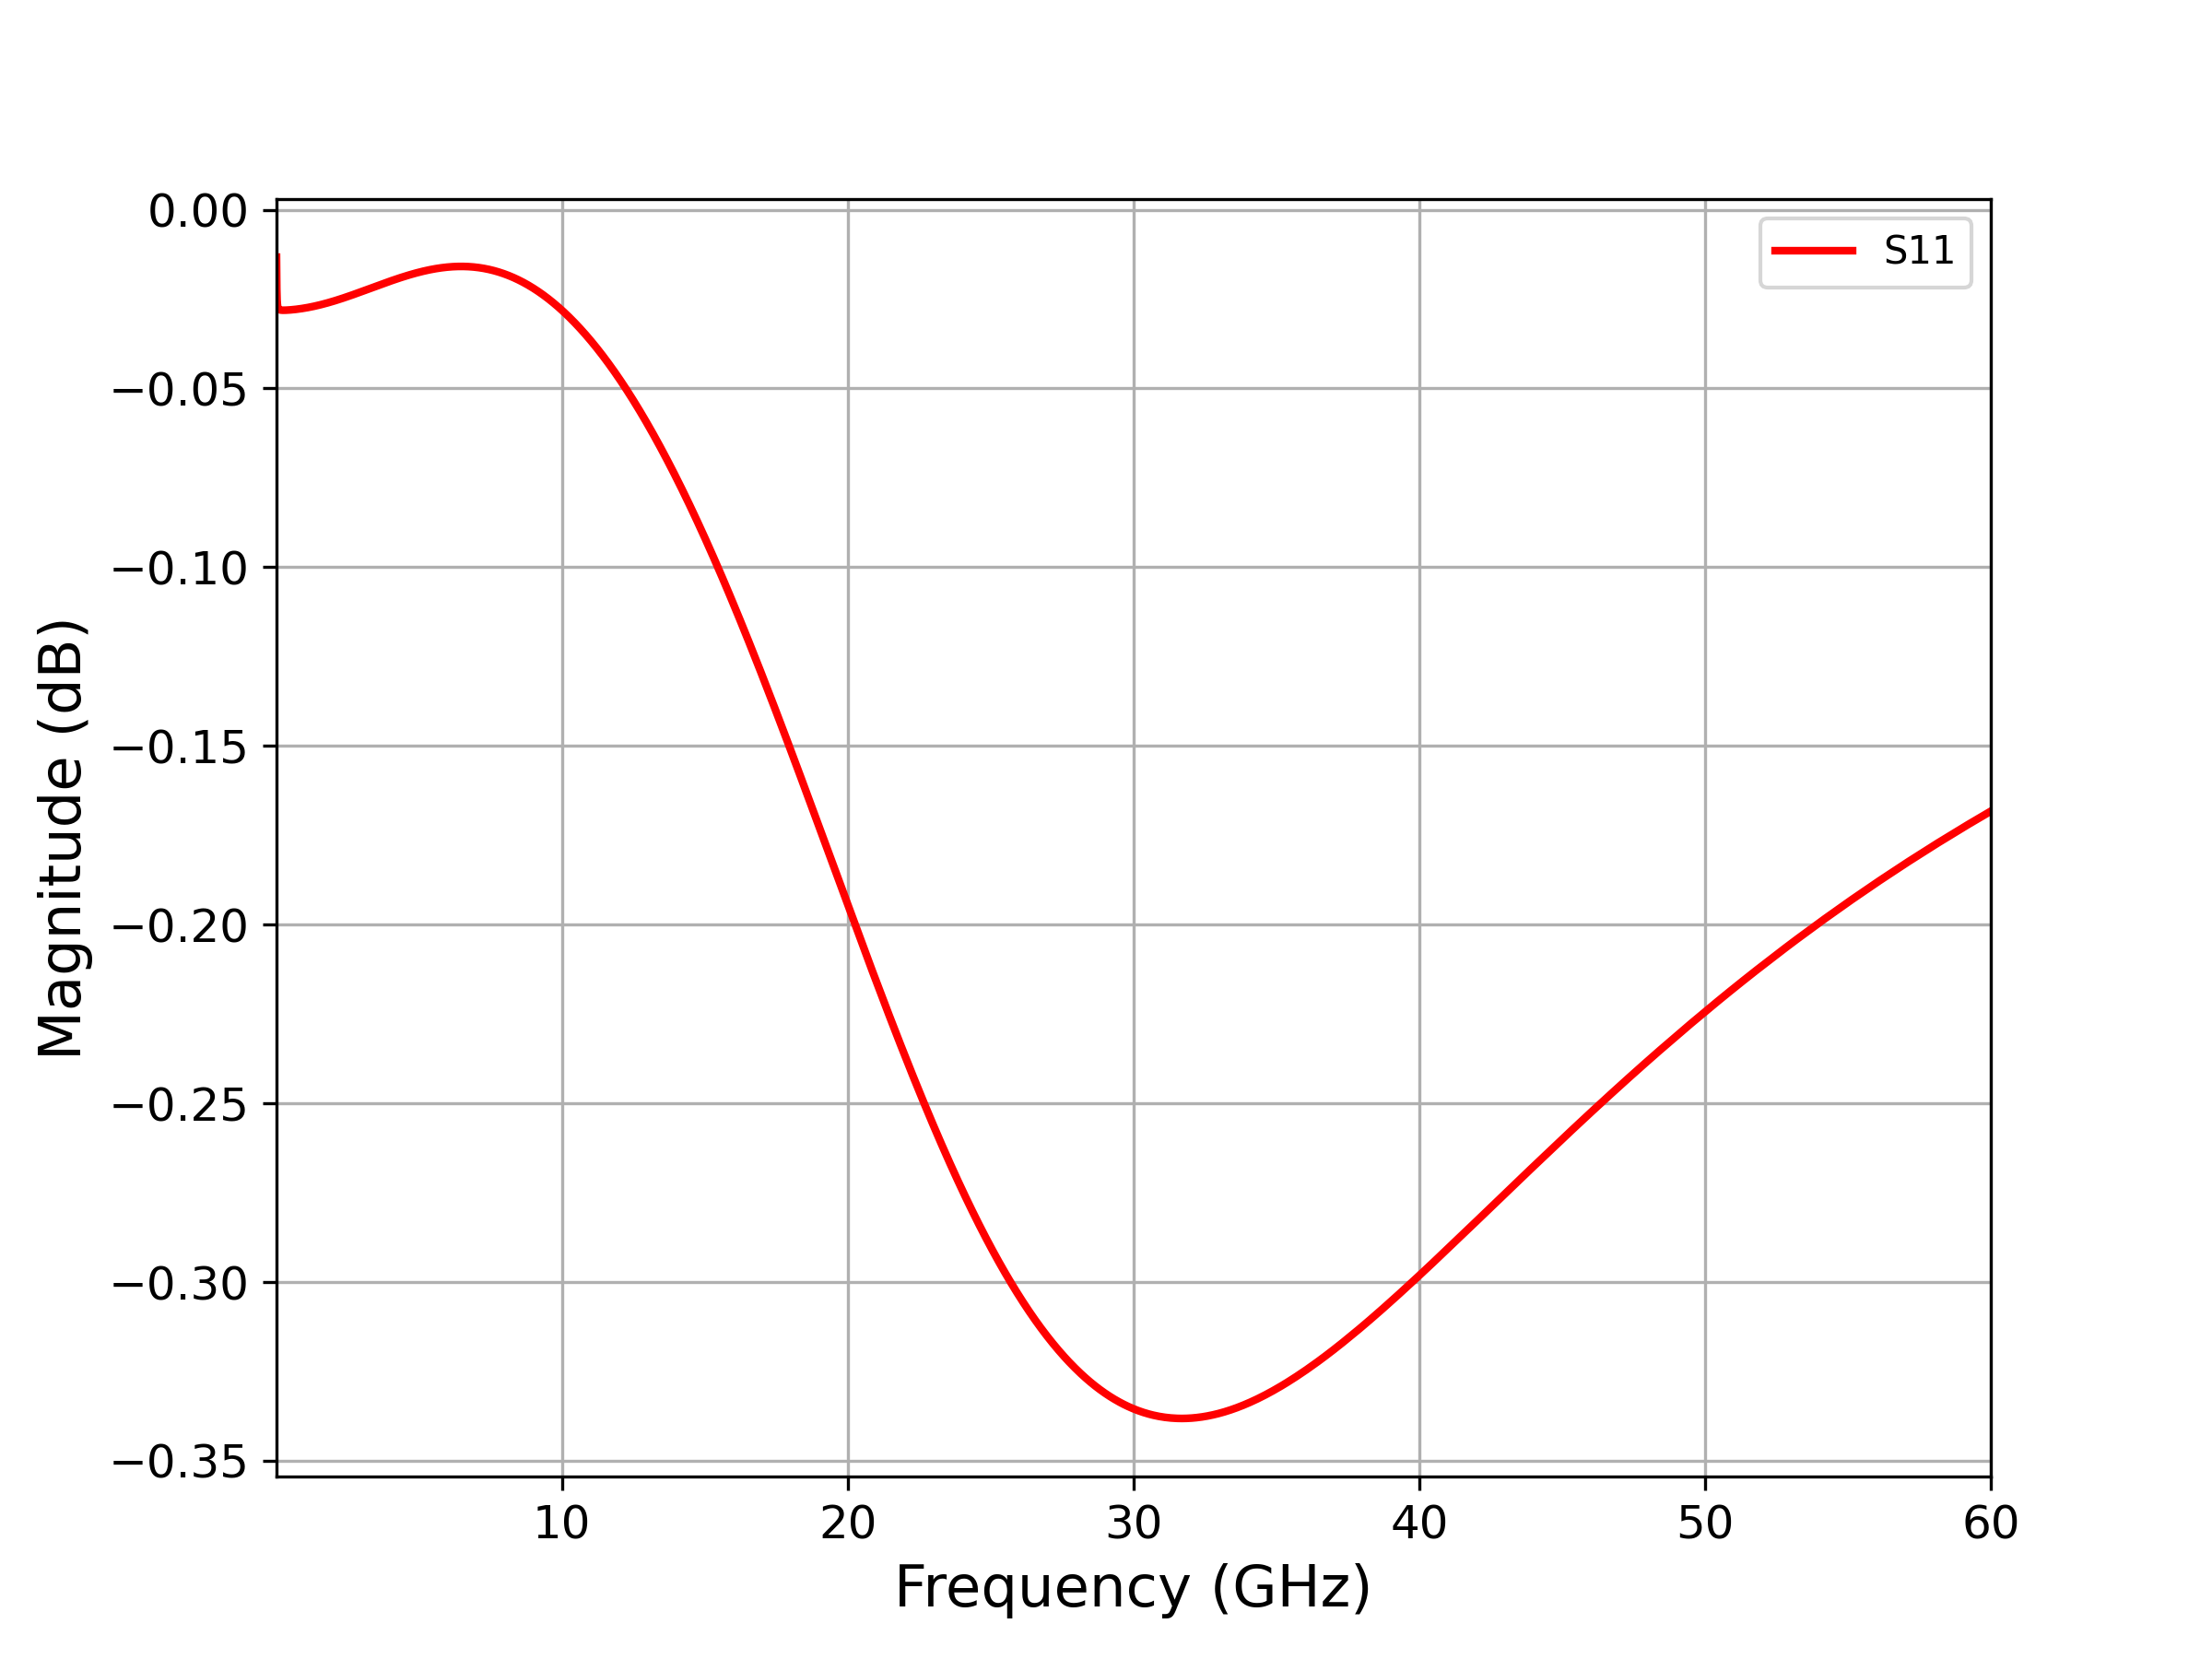
\includegraphics[]{figures/single_stage_s11.png}
%     }
%     \caption{$S_{11}$ parameter of a single-stage power amplifier (shown in Figure \ref{fig:single-stage-power-amplifier}) without matching network. The $S_{11}$ parameter is plotted from 0 GHz to 60 GHz.}
%     \label{fig:single-stage-without-cadence-s11}
% \end{figure}
% \begin{figure}[H]
%     \centering
%     \resizebox{0.8\textwidth}{!}{
%     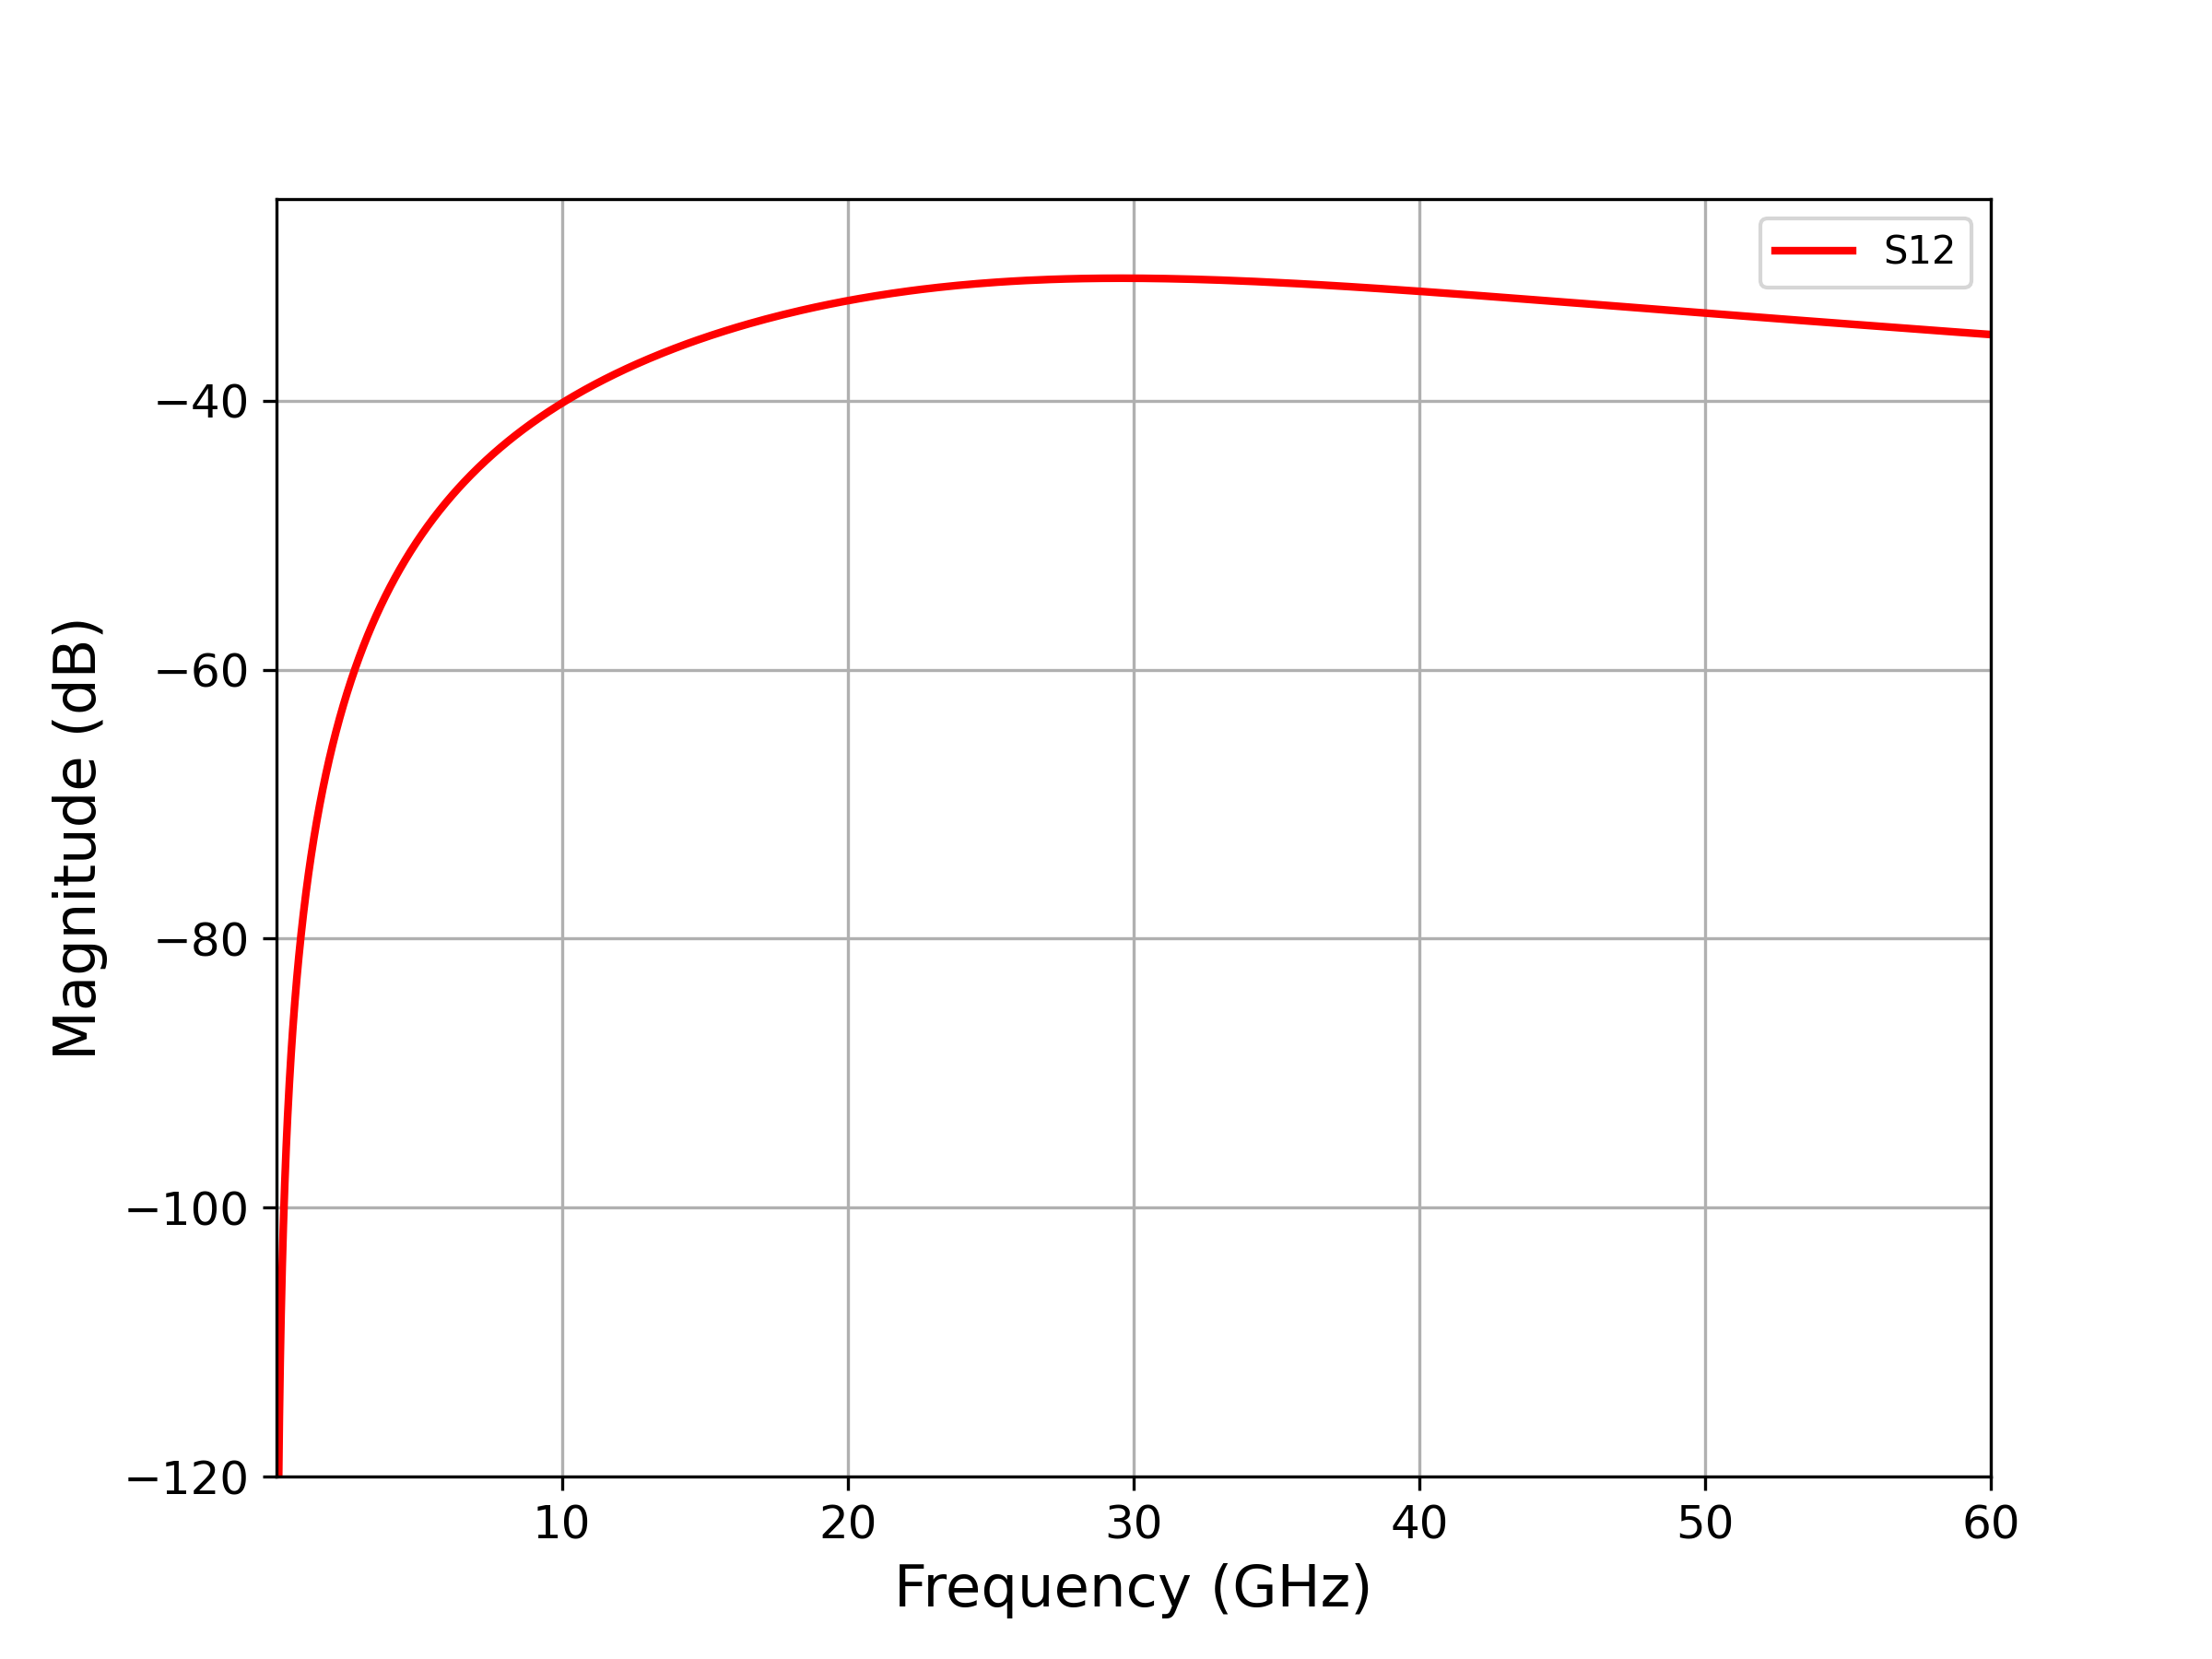
\includegraphics[]{figures/single_stage_s12.png}
%     }
%     \caption{$S_{12}$ parameter of a single-stage power amplifier (shown in Figure \ref{fig:single-stage-power-amplifier}) without matching network. The $S_{12}$ parameter is plotted from 0 GHz to 60 GHz.}
%     \label{fig:single-stage-without-cadence-s12}
% \end{figure}
\begin{figure}[H]
  \centering
  \begin{subfigure}{0.49\textwidth}
    \centering
    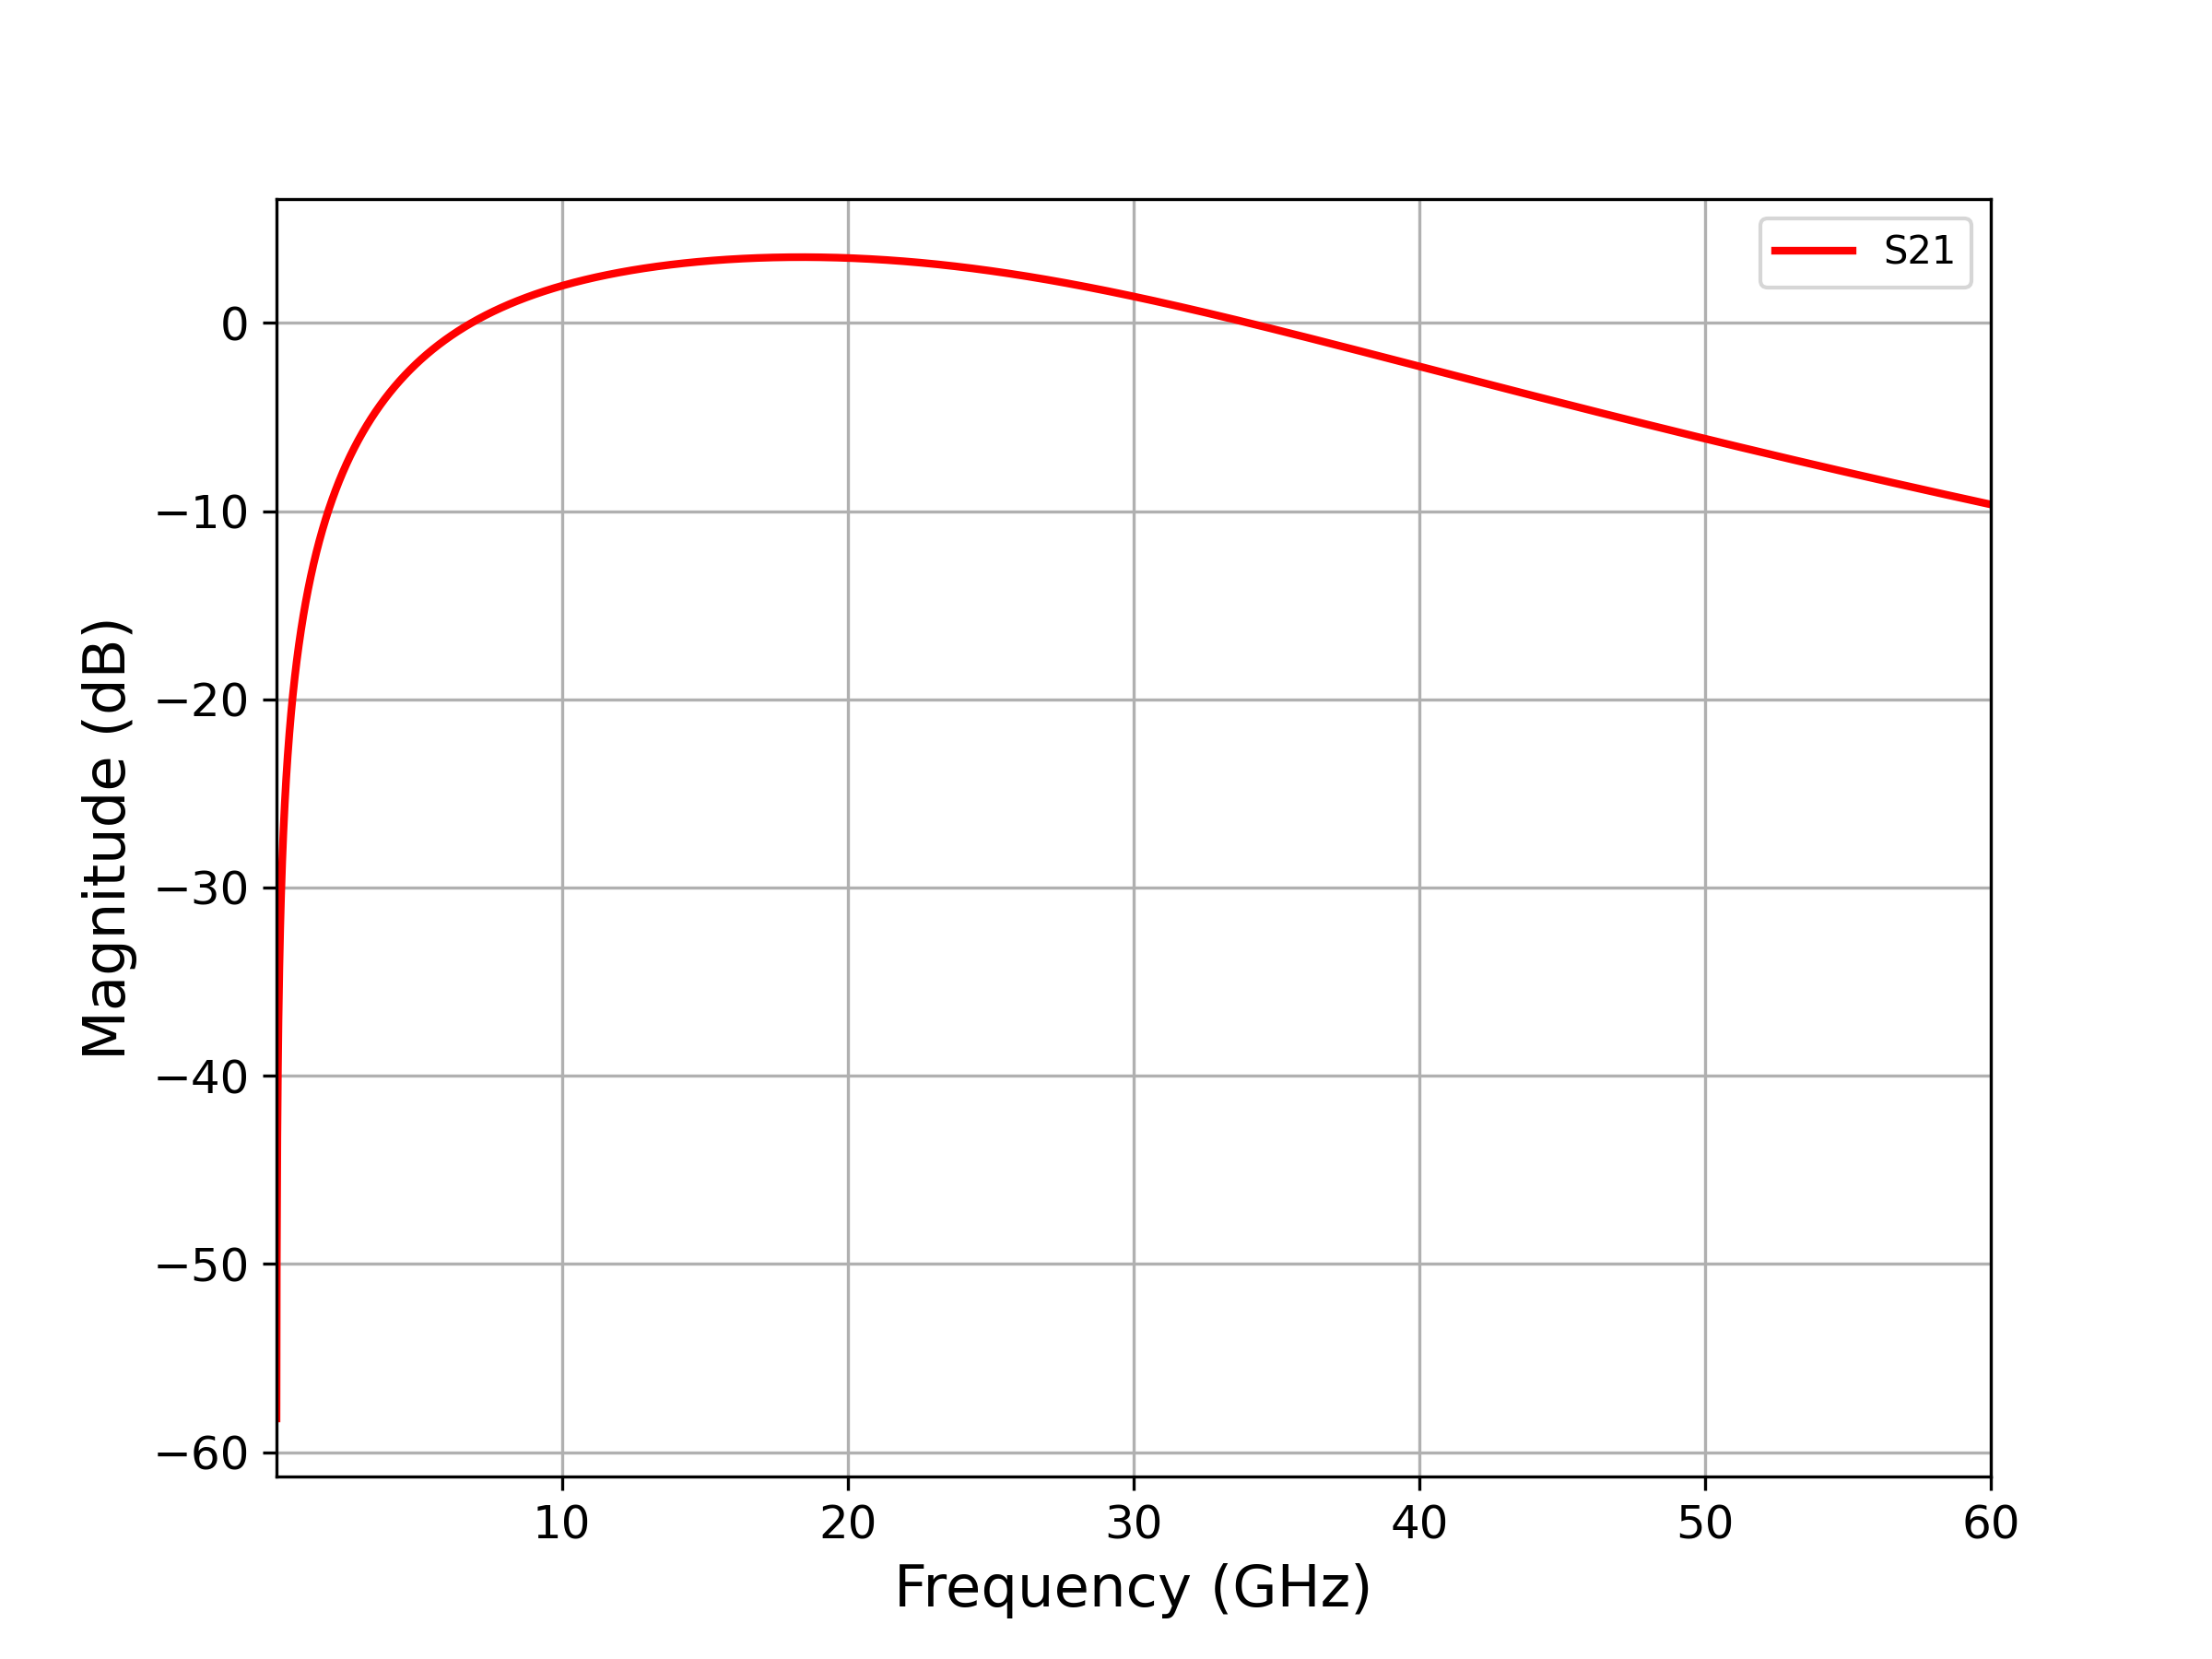
\includegraphics[width=\linewidth]{figures/single_stage_s21.png}
    \caption{}
    \label{fig:single-stage-without-cadence-s21}
  \end{subfigure}
  \hfill
  \begin{subfigure}{0.49\textwidth}
    \centering
    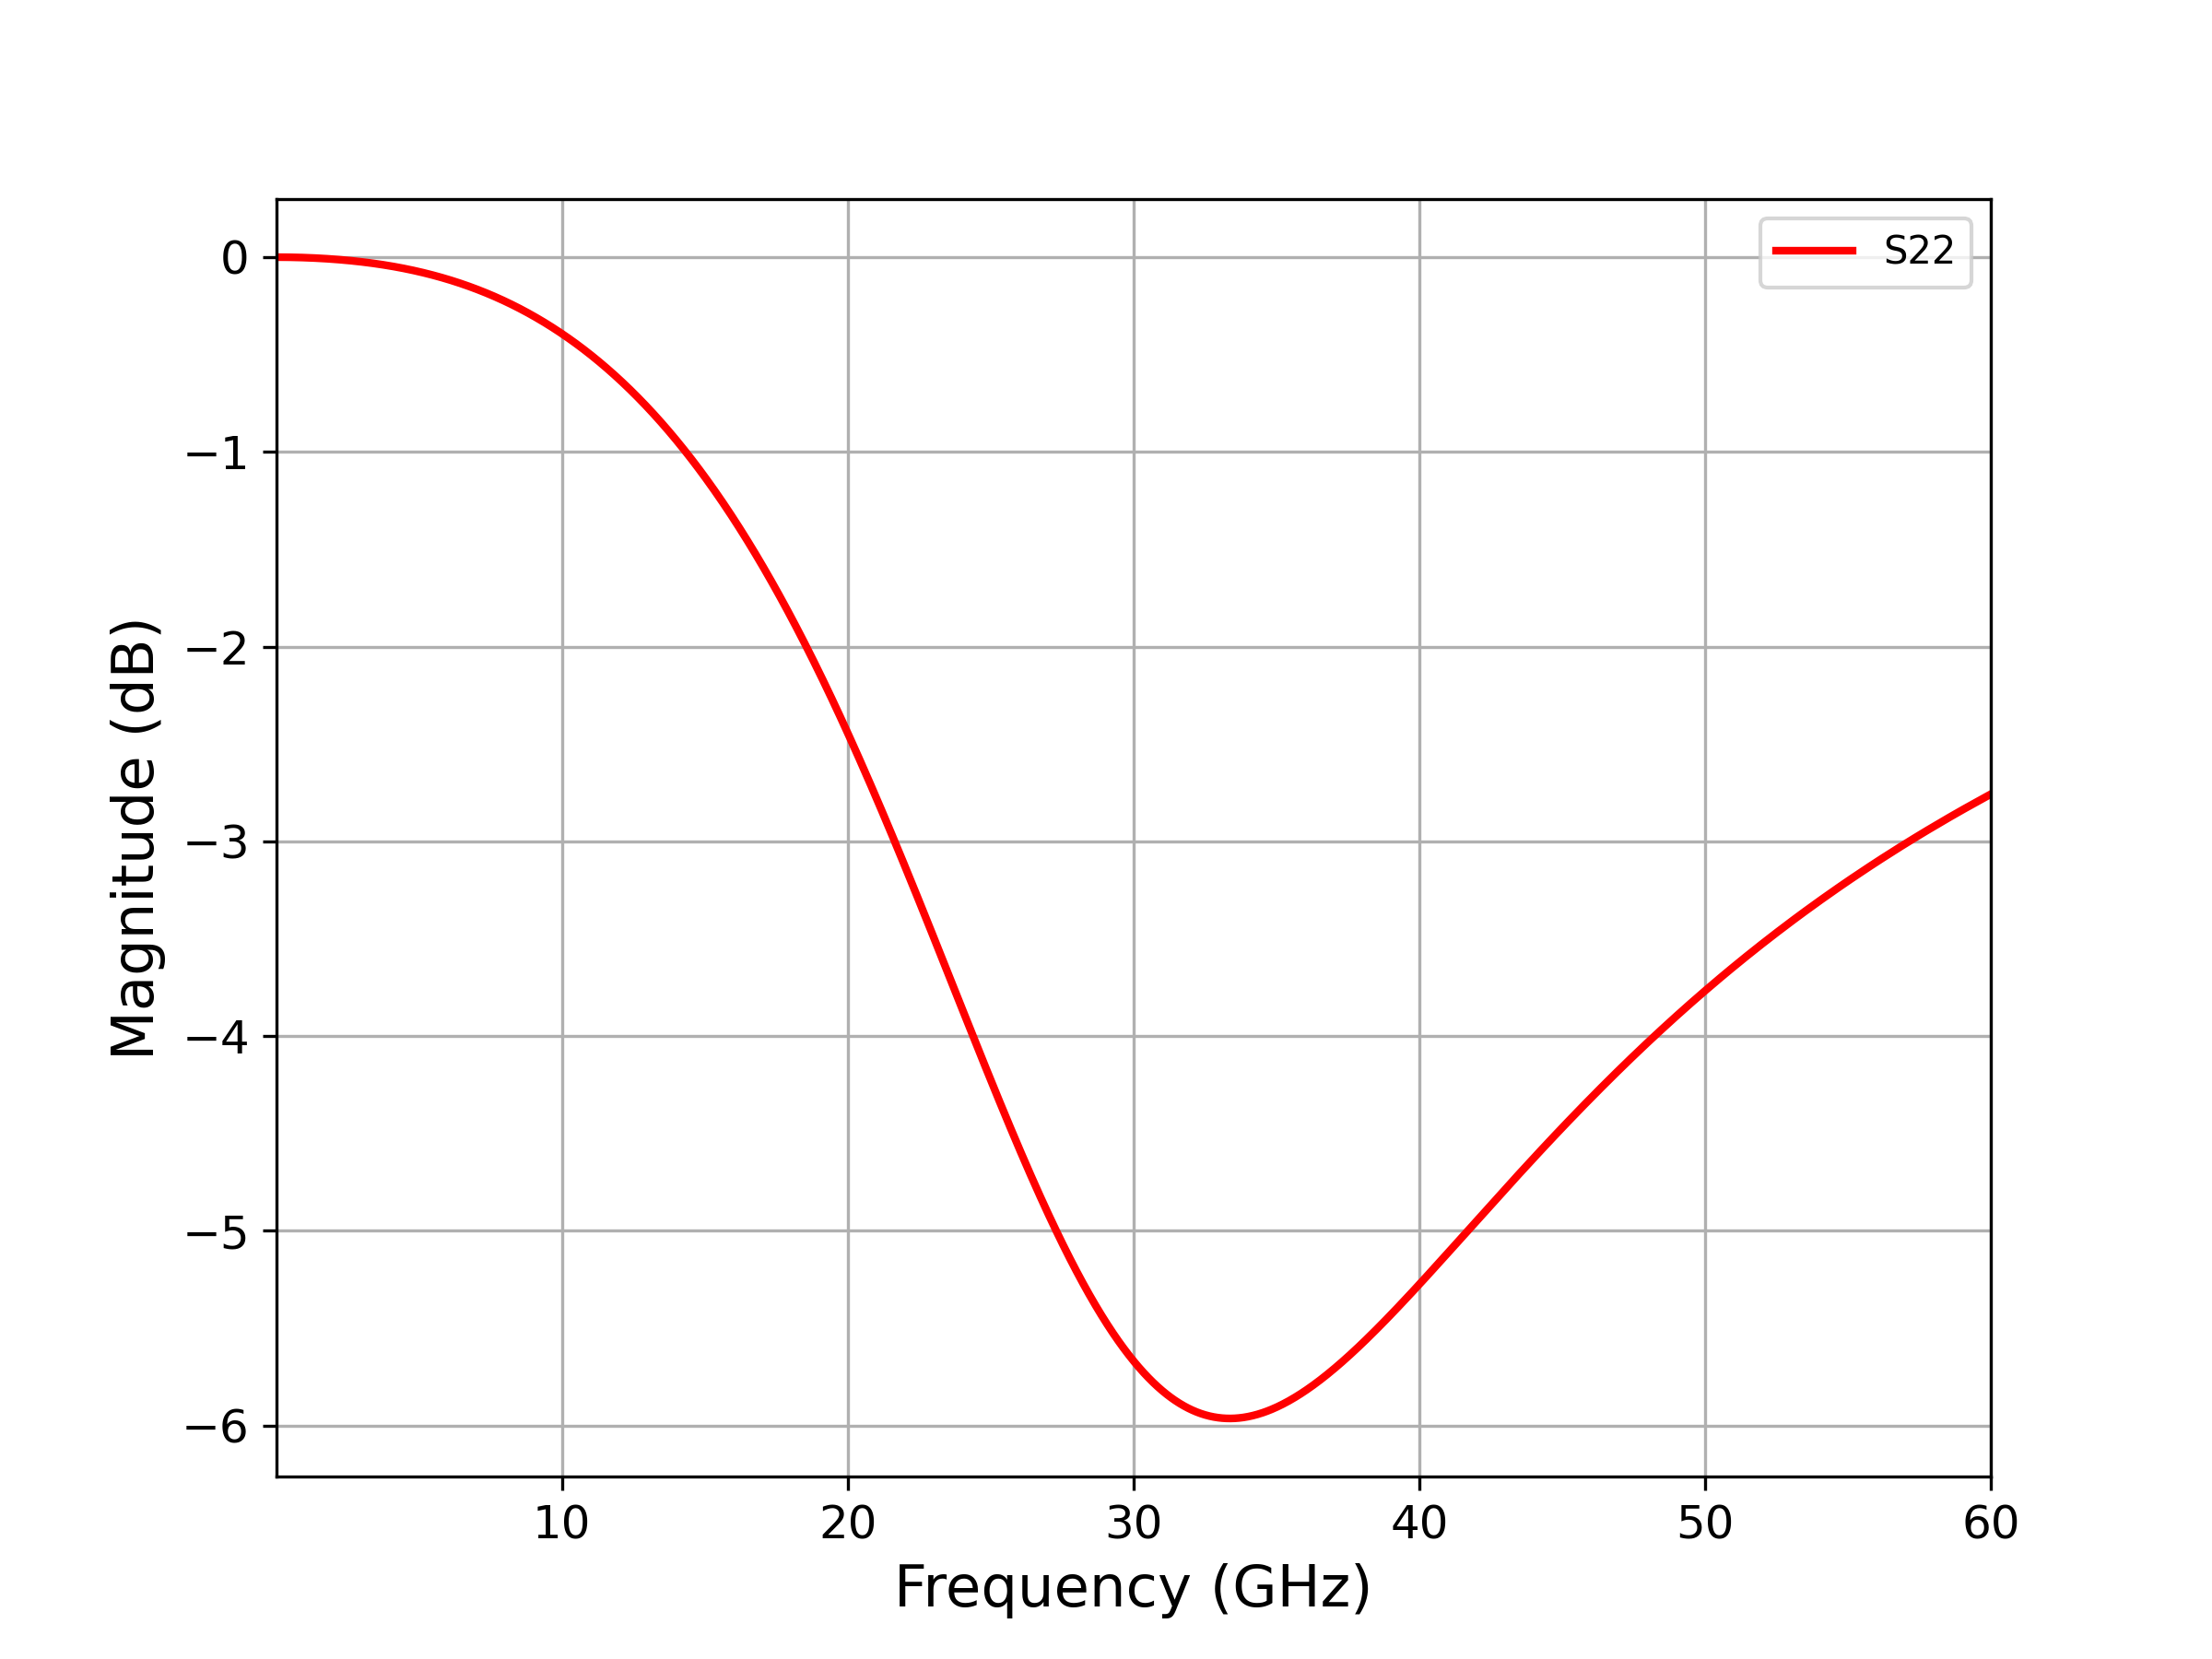
\includegraphics[width=\linewidth]{figures/single_stage_s22.png}
    \caption{}
     \label{fig:single-stage-without-cadence-s22}
  \end{subfigure}
  \caption{(a) $S_{21}$ parameter of a single-stage power amplifier (shown in Figure \ref{fig:single-stage-power-amplifier}) without matching network. (b) $S_{22}$ parameter of a single-stage power amplifier (shown in Figure \ref{fig:single-stage-power-amplifier}) without matching network.}
  \label{fig:single-stage-without-cadence-s21-s22}
\end{figure}

The maximum value of $S_{21}$ of a single-stage power amplifier is 3.78 dB at resonance frequency 18 GHz, which indicates poor power gain, which is not enough for real-life applications. The $S_{22}$ parameter is a measure of how well the power amplifier matches the impedance at its output. A lower magnitude of 
$S_{22}$ indicates a better match between the output impedance of the power amplifier and the load impedance, resulting in less power being reflected back. A higher magnitude indicates a higher level of reflection and poor impedance matching. The value of $S_{22}$ of single-stage PA is -1.9 dB at 18 GHz, which is insufficient for an output-matching network. 
% \begin{figure}[H]
%     \centering
%     \resizebox{0.8\textwidth}{!}{
%     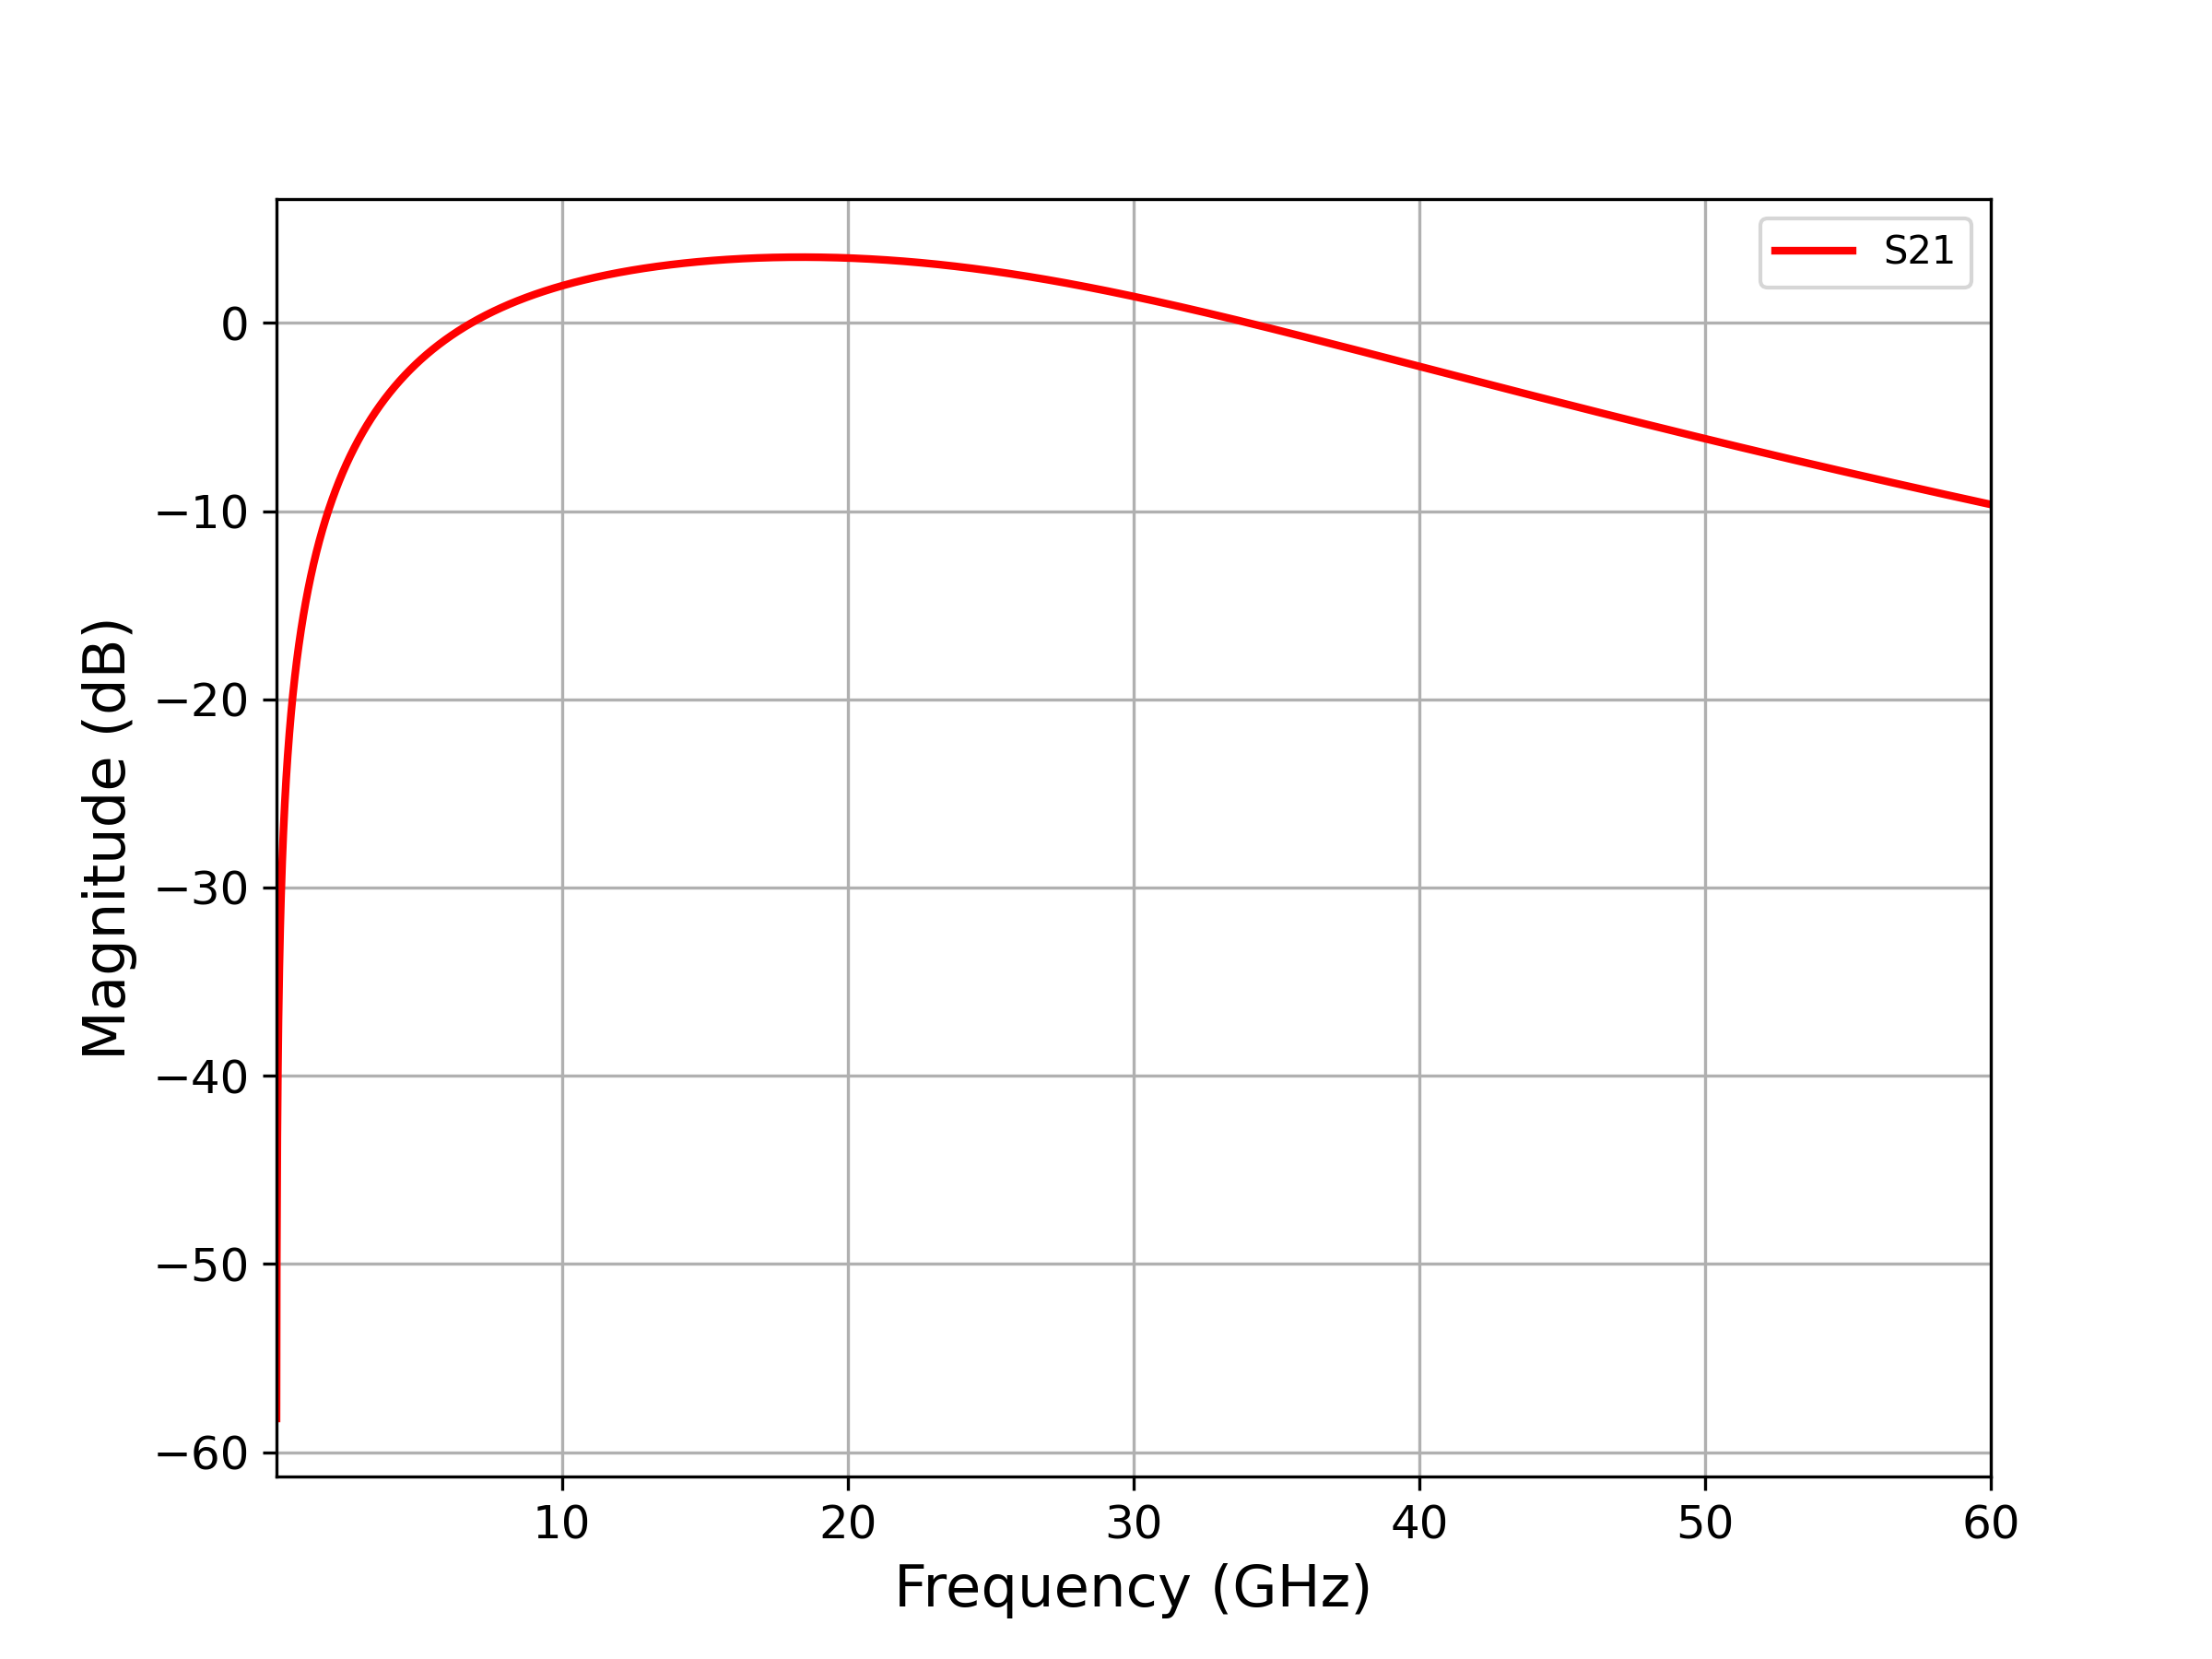
\includegraphics[]{figures/single_stage_s21.png}
%     }
%     \caption{$S_{21}$ parameter of a single-stage power amplifier (shown in Figure \ref{fig:single-stage-power-amplifier}) without matching network. The $S_{21}$ parameter is plotted from 0 GHz to 60 GHz.}
%     \label{fig:single-stage-without-cadence-s21}
% \end{figure}
% \begin{figure}[H]
%     \centering
%     \resizebox{0.8\textwidth}{!}{
%     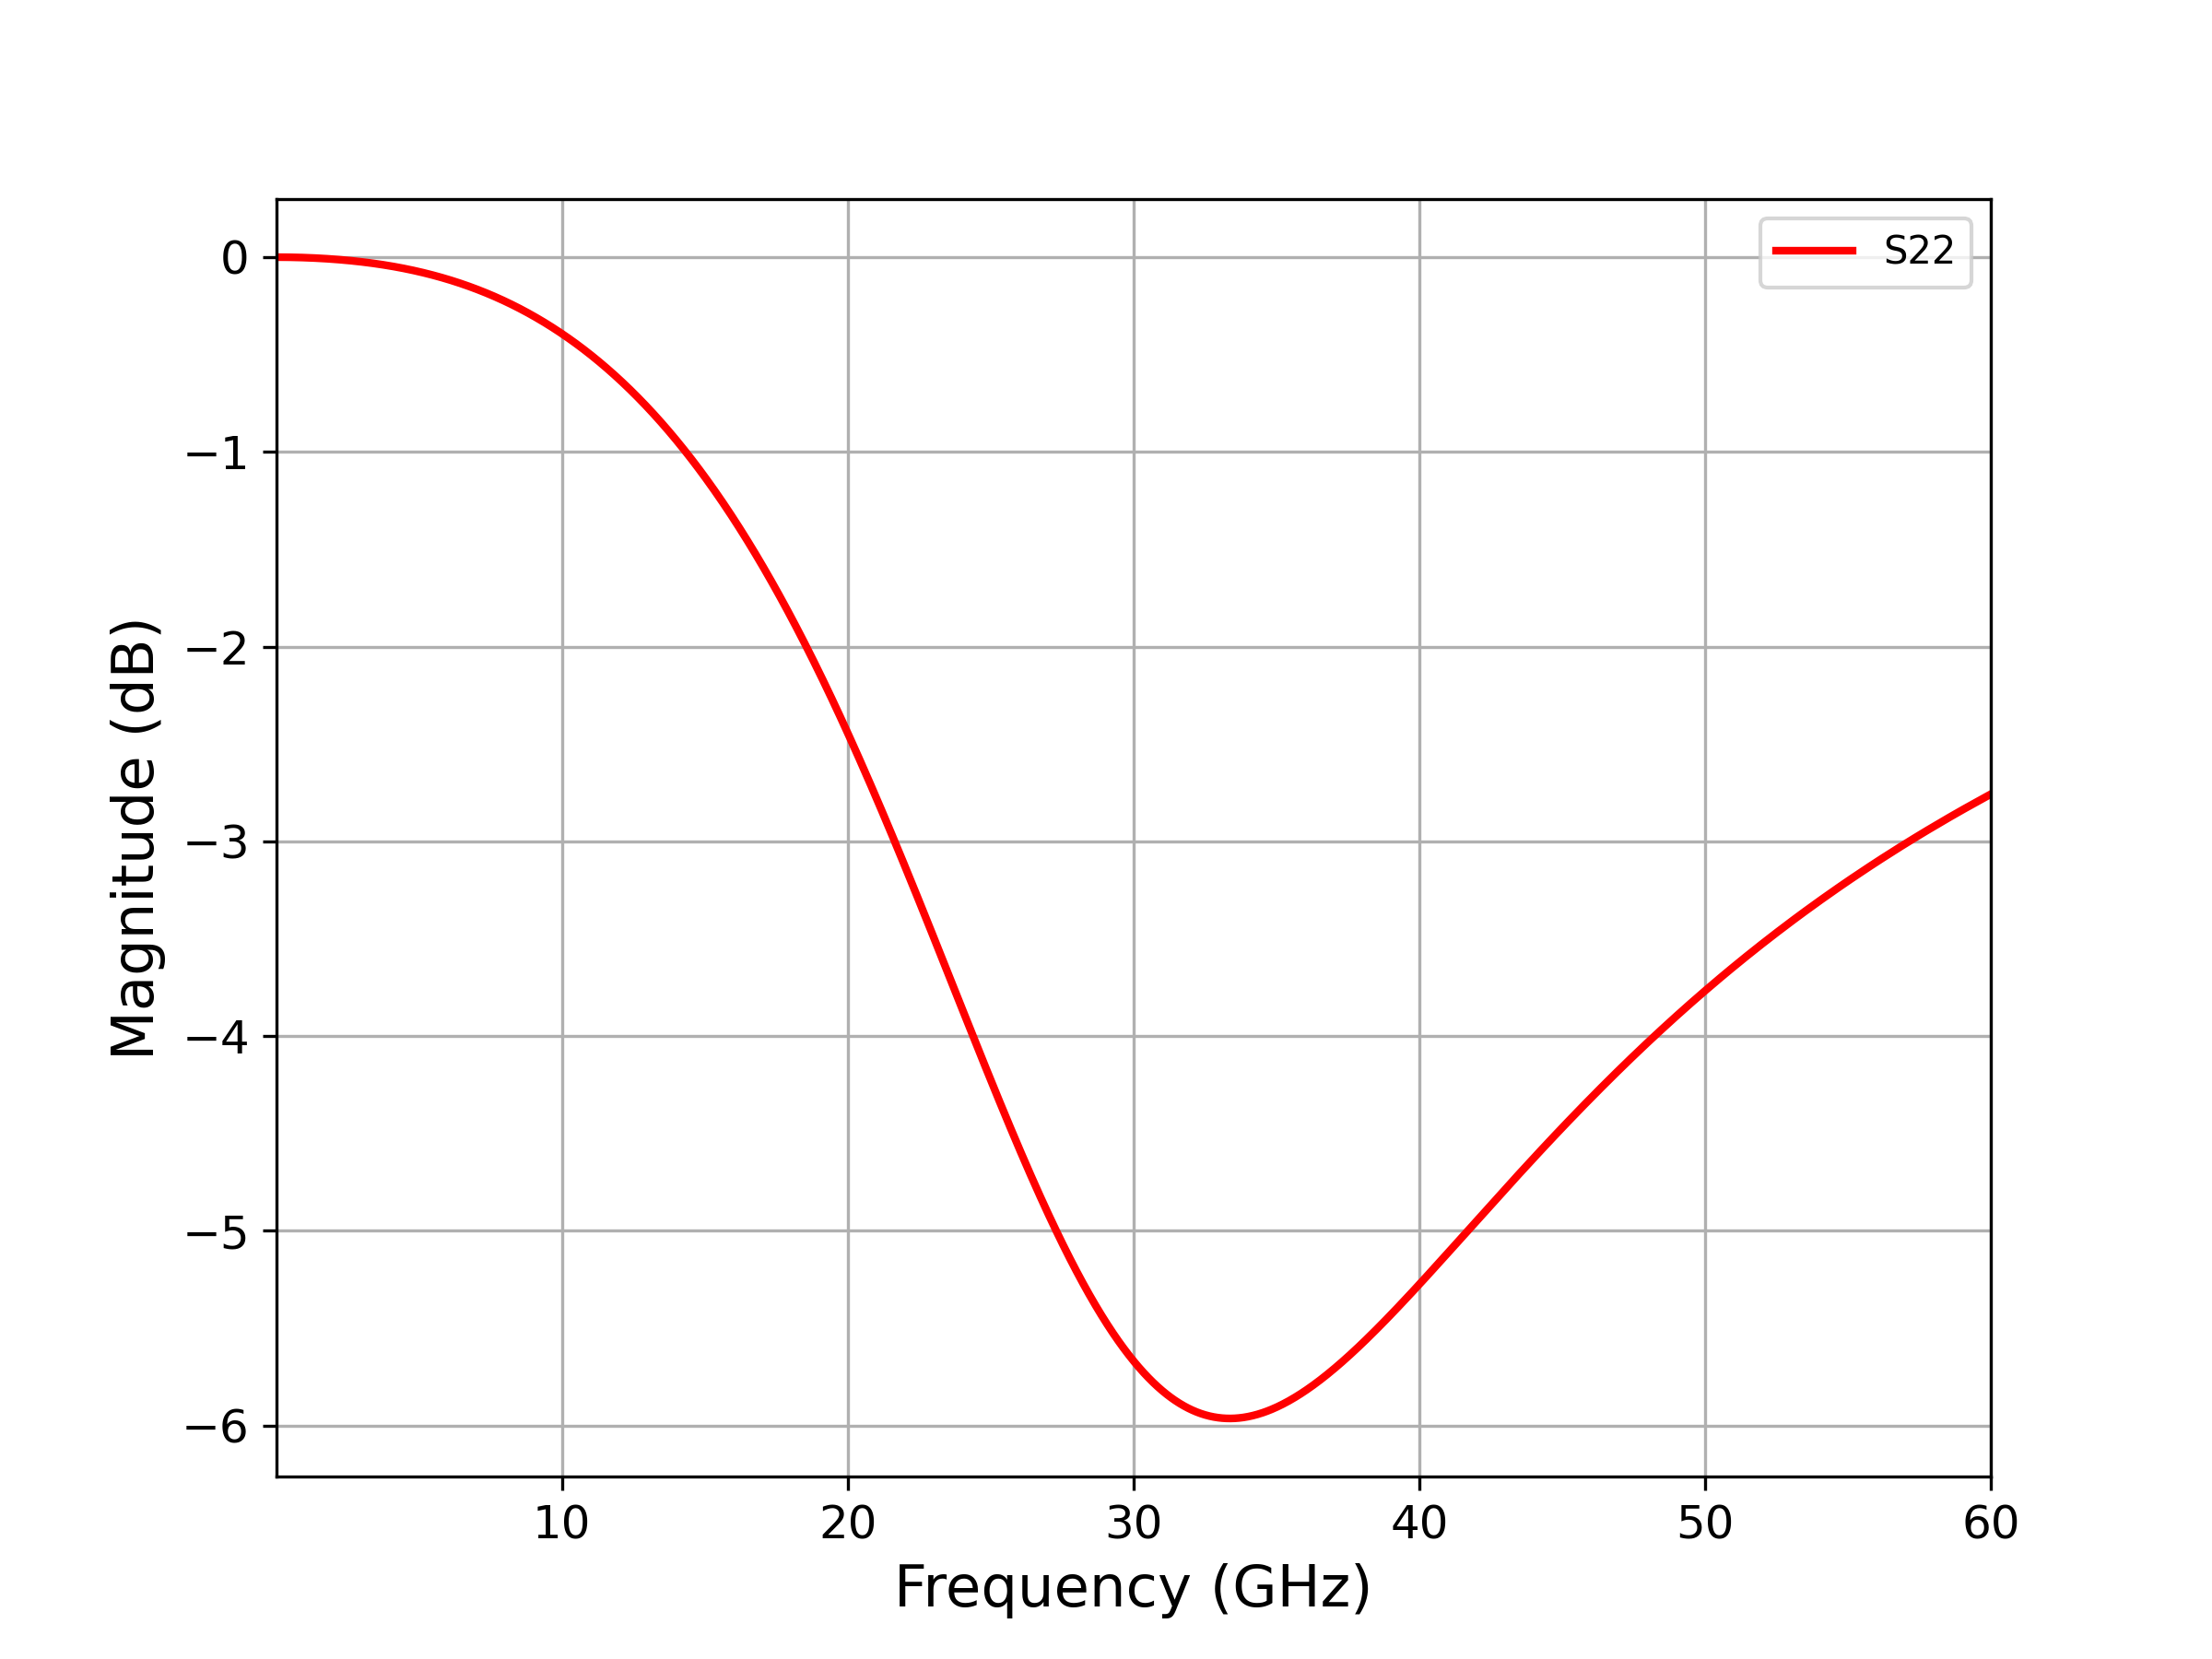
\includegraphics[]{figures/single_stage_s22.png}
%     }
%     \caption{$S_{22}$ parameter of a single-stage power amplifier (shown in Figure \ref{fig:single-stage-power-amplifier}) without matching network. The $S_{22}$ parameter is plotted from 0 GHz to 60 GHz.}
%     \label{fig:single-stage-without-cadence-s22}
% \end{figure}

%The $S$ parameter simulation of two stage power amplifier(Figure \ref{fig:double-stage-power-amplifier}) is shown below
\begin{figure}[H]
  \centering
  \begin{subfigure}{0.49\textwidth}
    \centering
    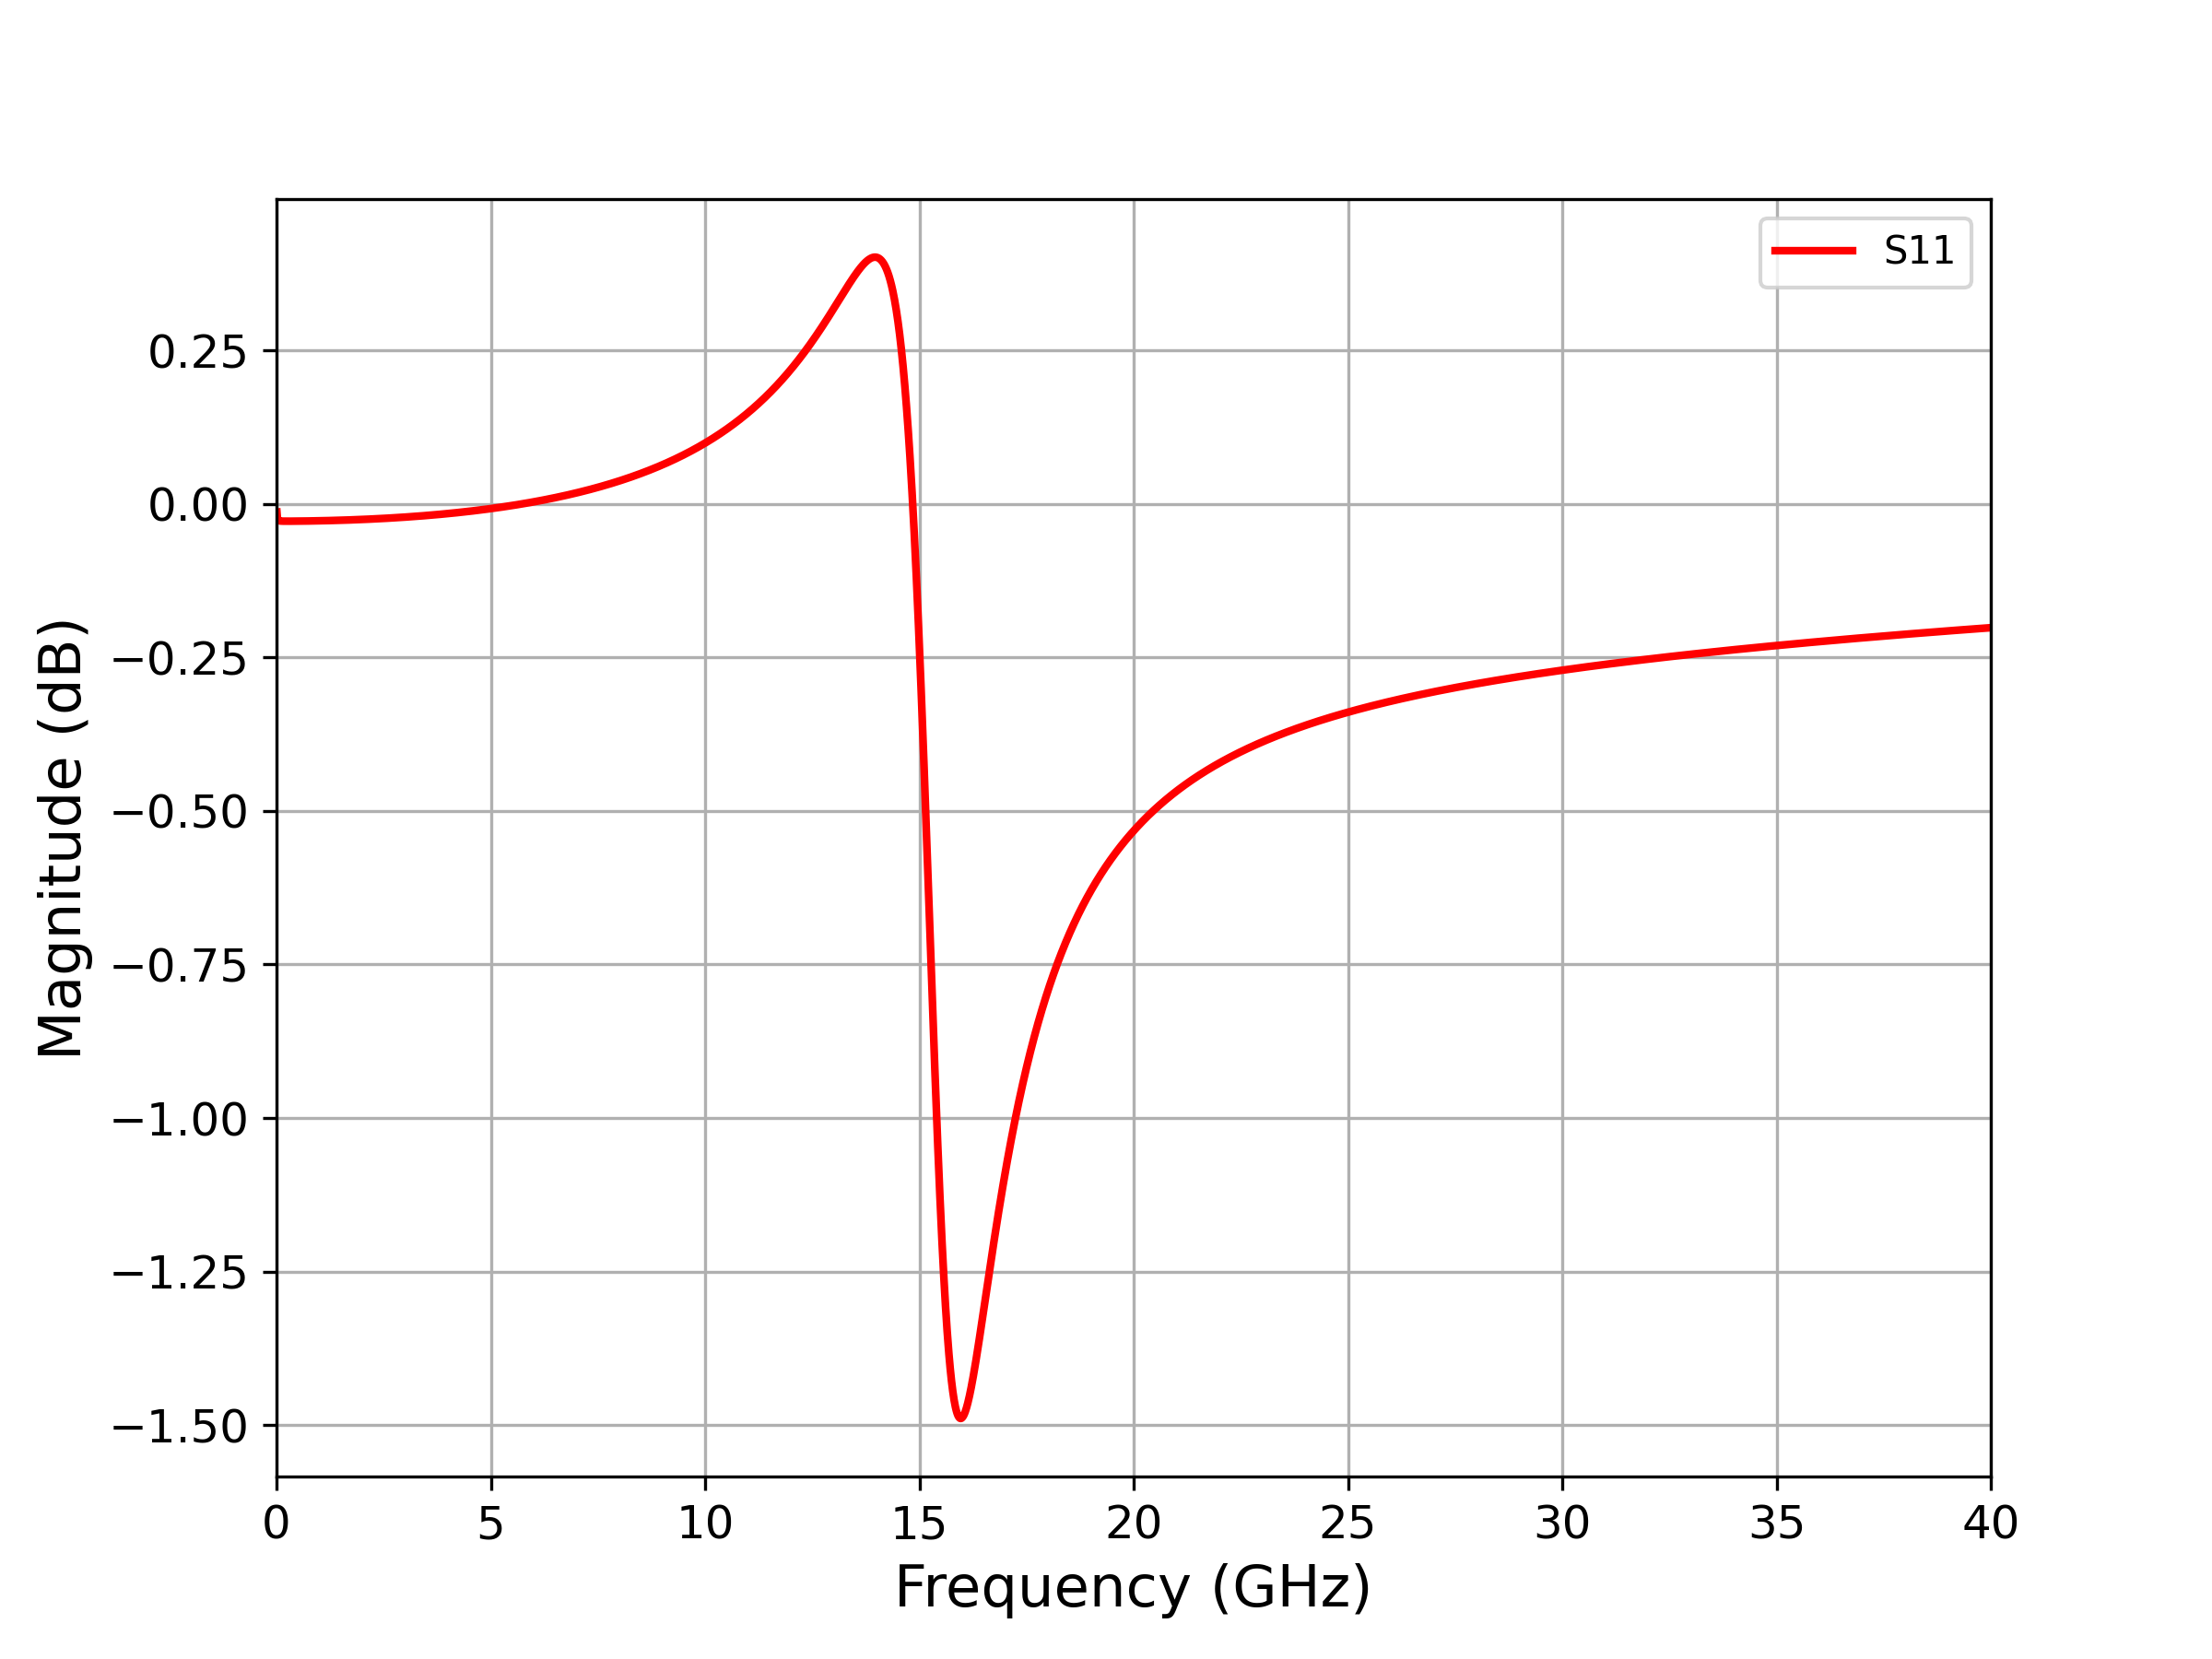
\includegraphics[width=\linewidth]{figures/two_stage_s11.png}
    \caption{}
    \label{fig:two-stage-without-cadence-s11}
  \end{subfigure}
  \hfill
  \begin{subfigure}{0.49\textwidth}
    \centering
    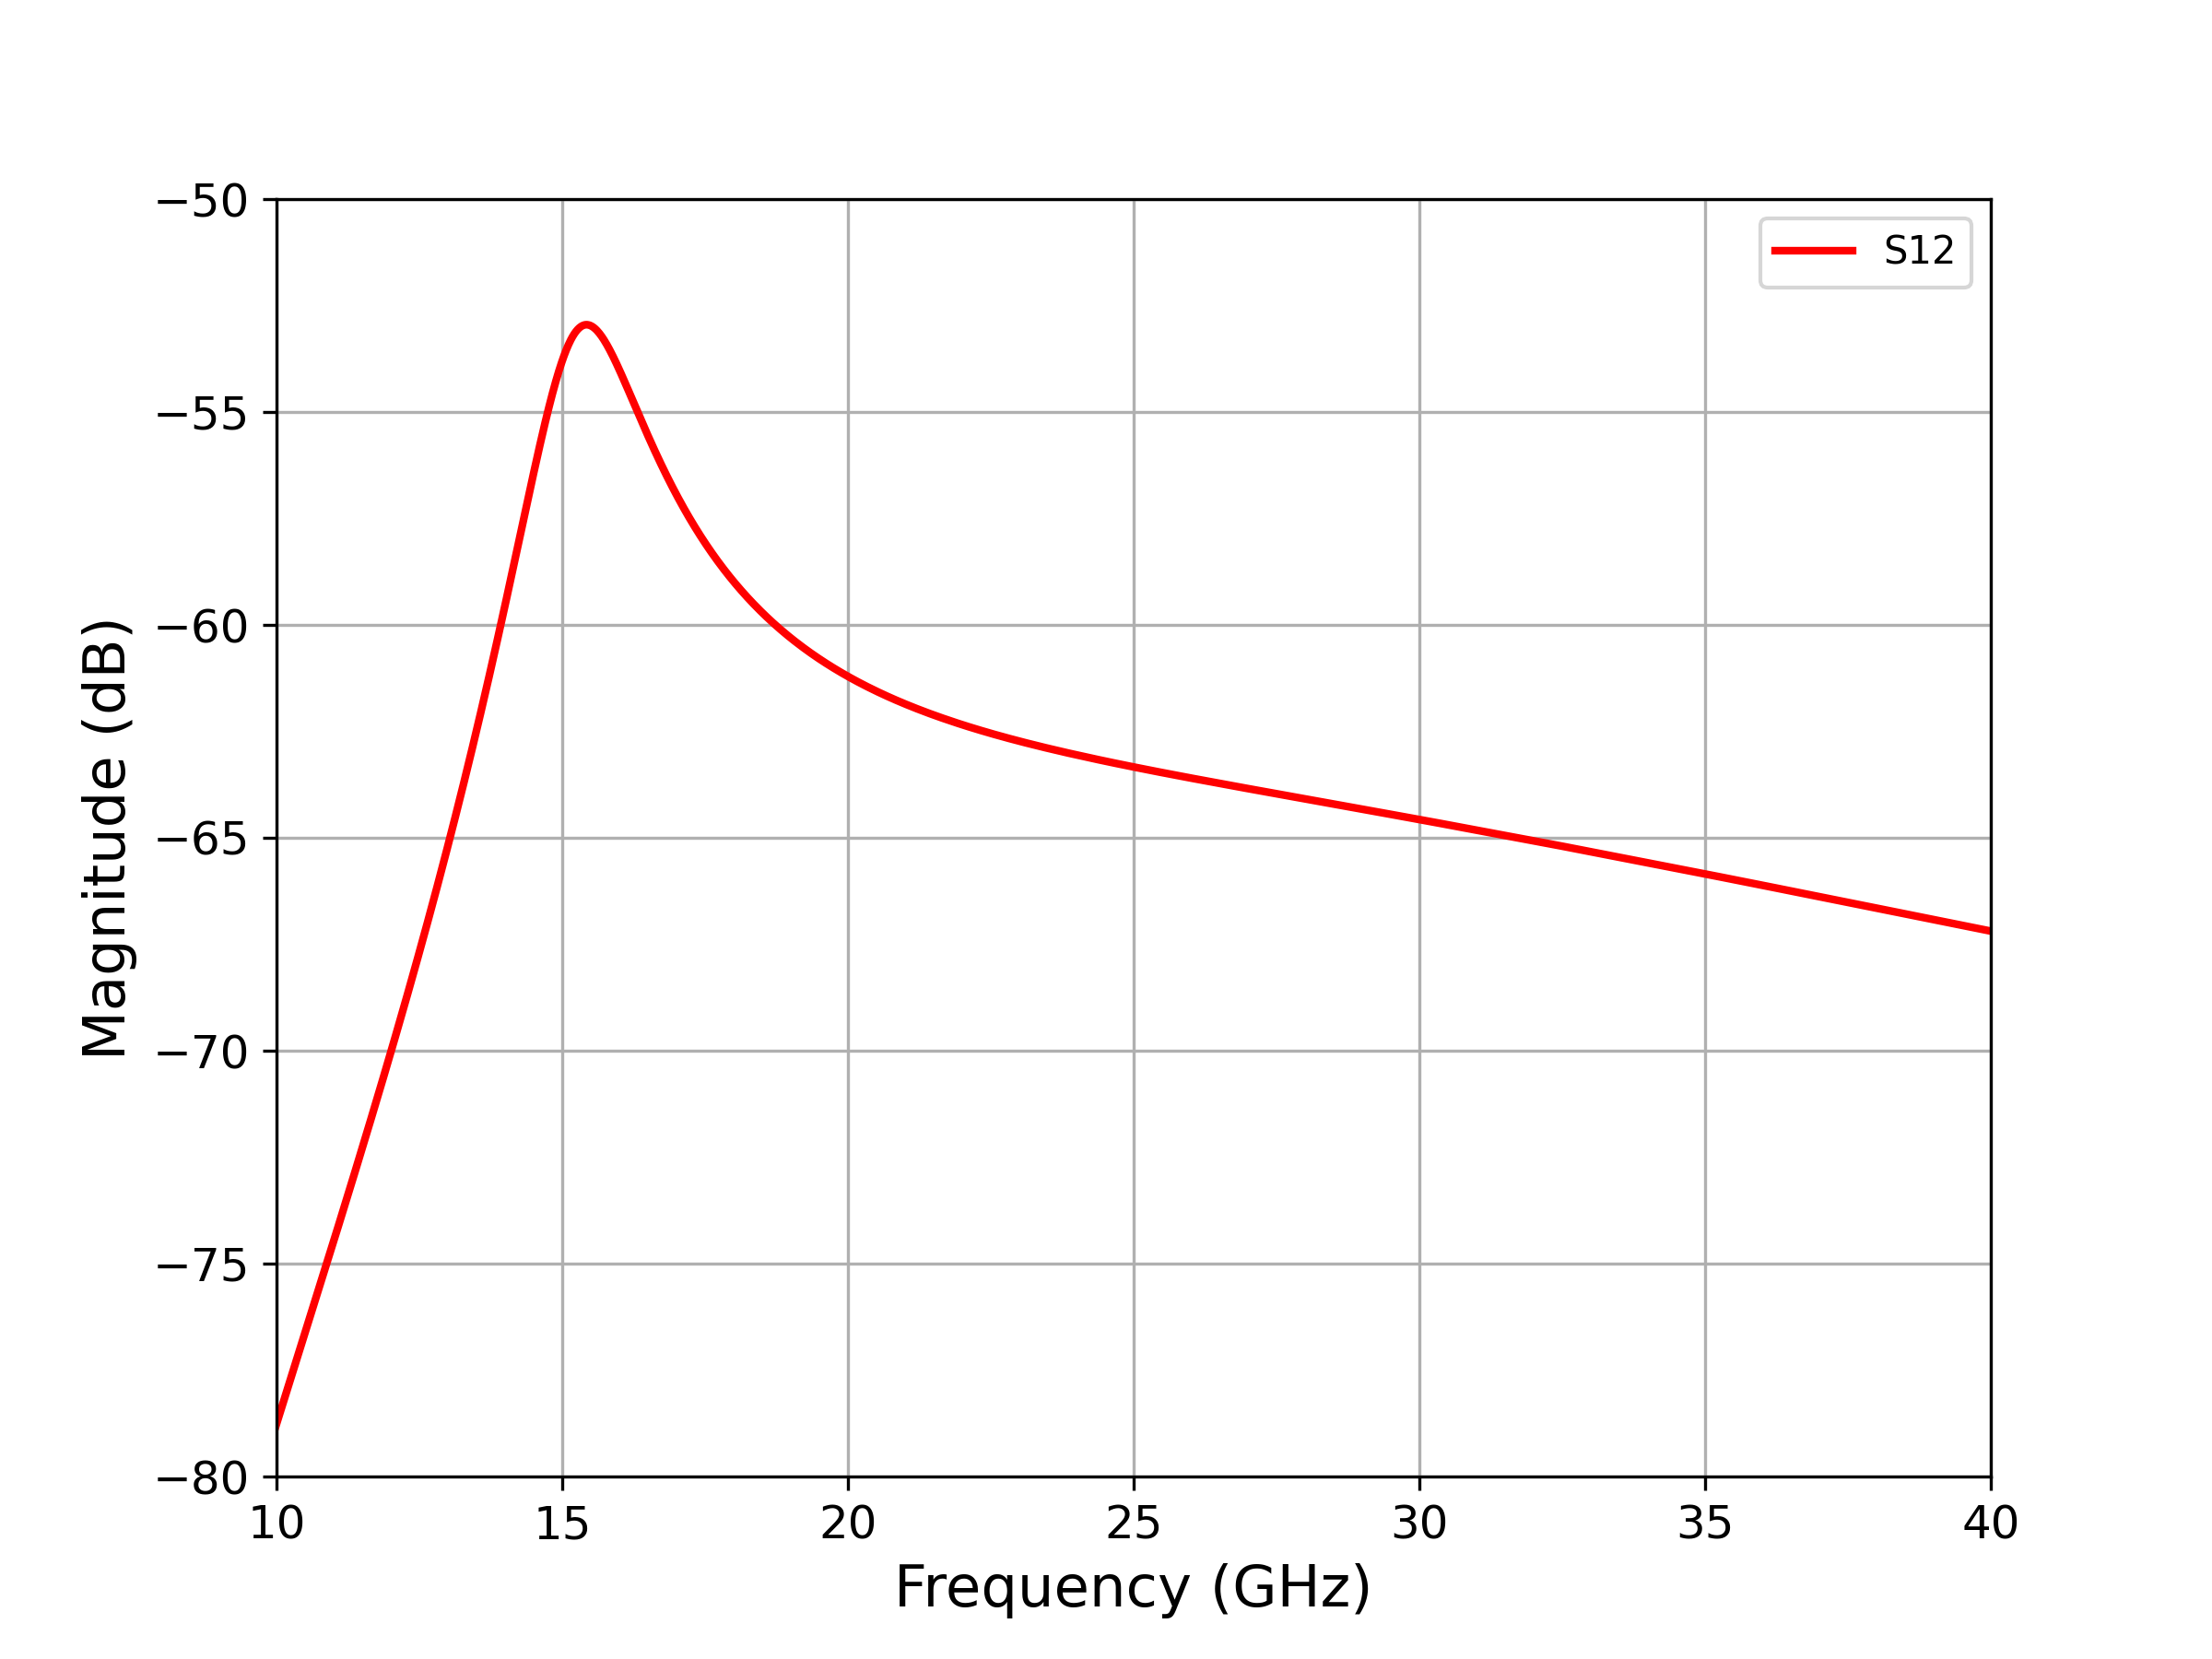
\includegraphics[width=\linewidth]{figures/two_stage_s12.png}
    \caption{}
     \label{fig:two-stage-without-cadence-s12}
  \end{subfigure}
  \caption{(a) $S_{11}$ parameter of a two-stage power amplifier (shown in Figure \ref{fig:double-stage-power-amplifier}) without matching network. (b) $S_{12}$ parameter of a two-stage power amplifier (shown in Figure \ref{fig:double-stage-power-amplifier}) without matching network.}
  \label{fig:two-stage-without-cadence-s11-s12}
\end{figure}

To increase gain and bandwidth, a second stage was introduced with the first stage. Now the value of $S_{11}$ is -1.5 dB at 15 GHz, which means the matching is improved compared with a single-stage power amplifier. The value of input return loss ($S_{12}$) is less than -50 dB throughout the BW.
% \begin{figure}[H]
%     \centering
%     \resizebox{0.8\textwidth}{!}{
%     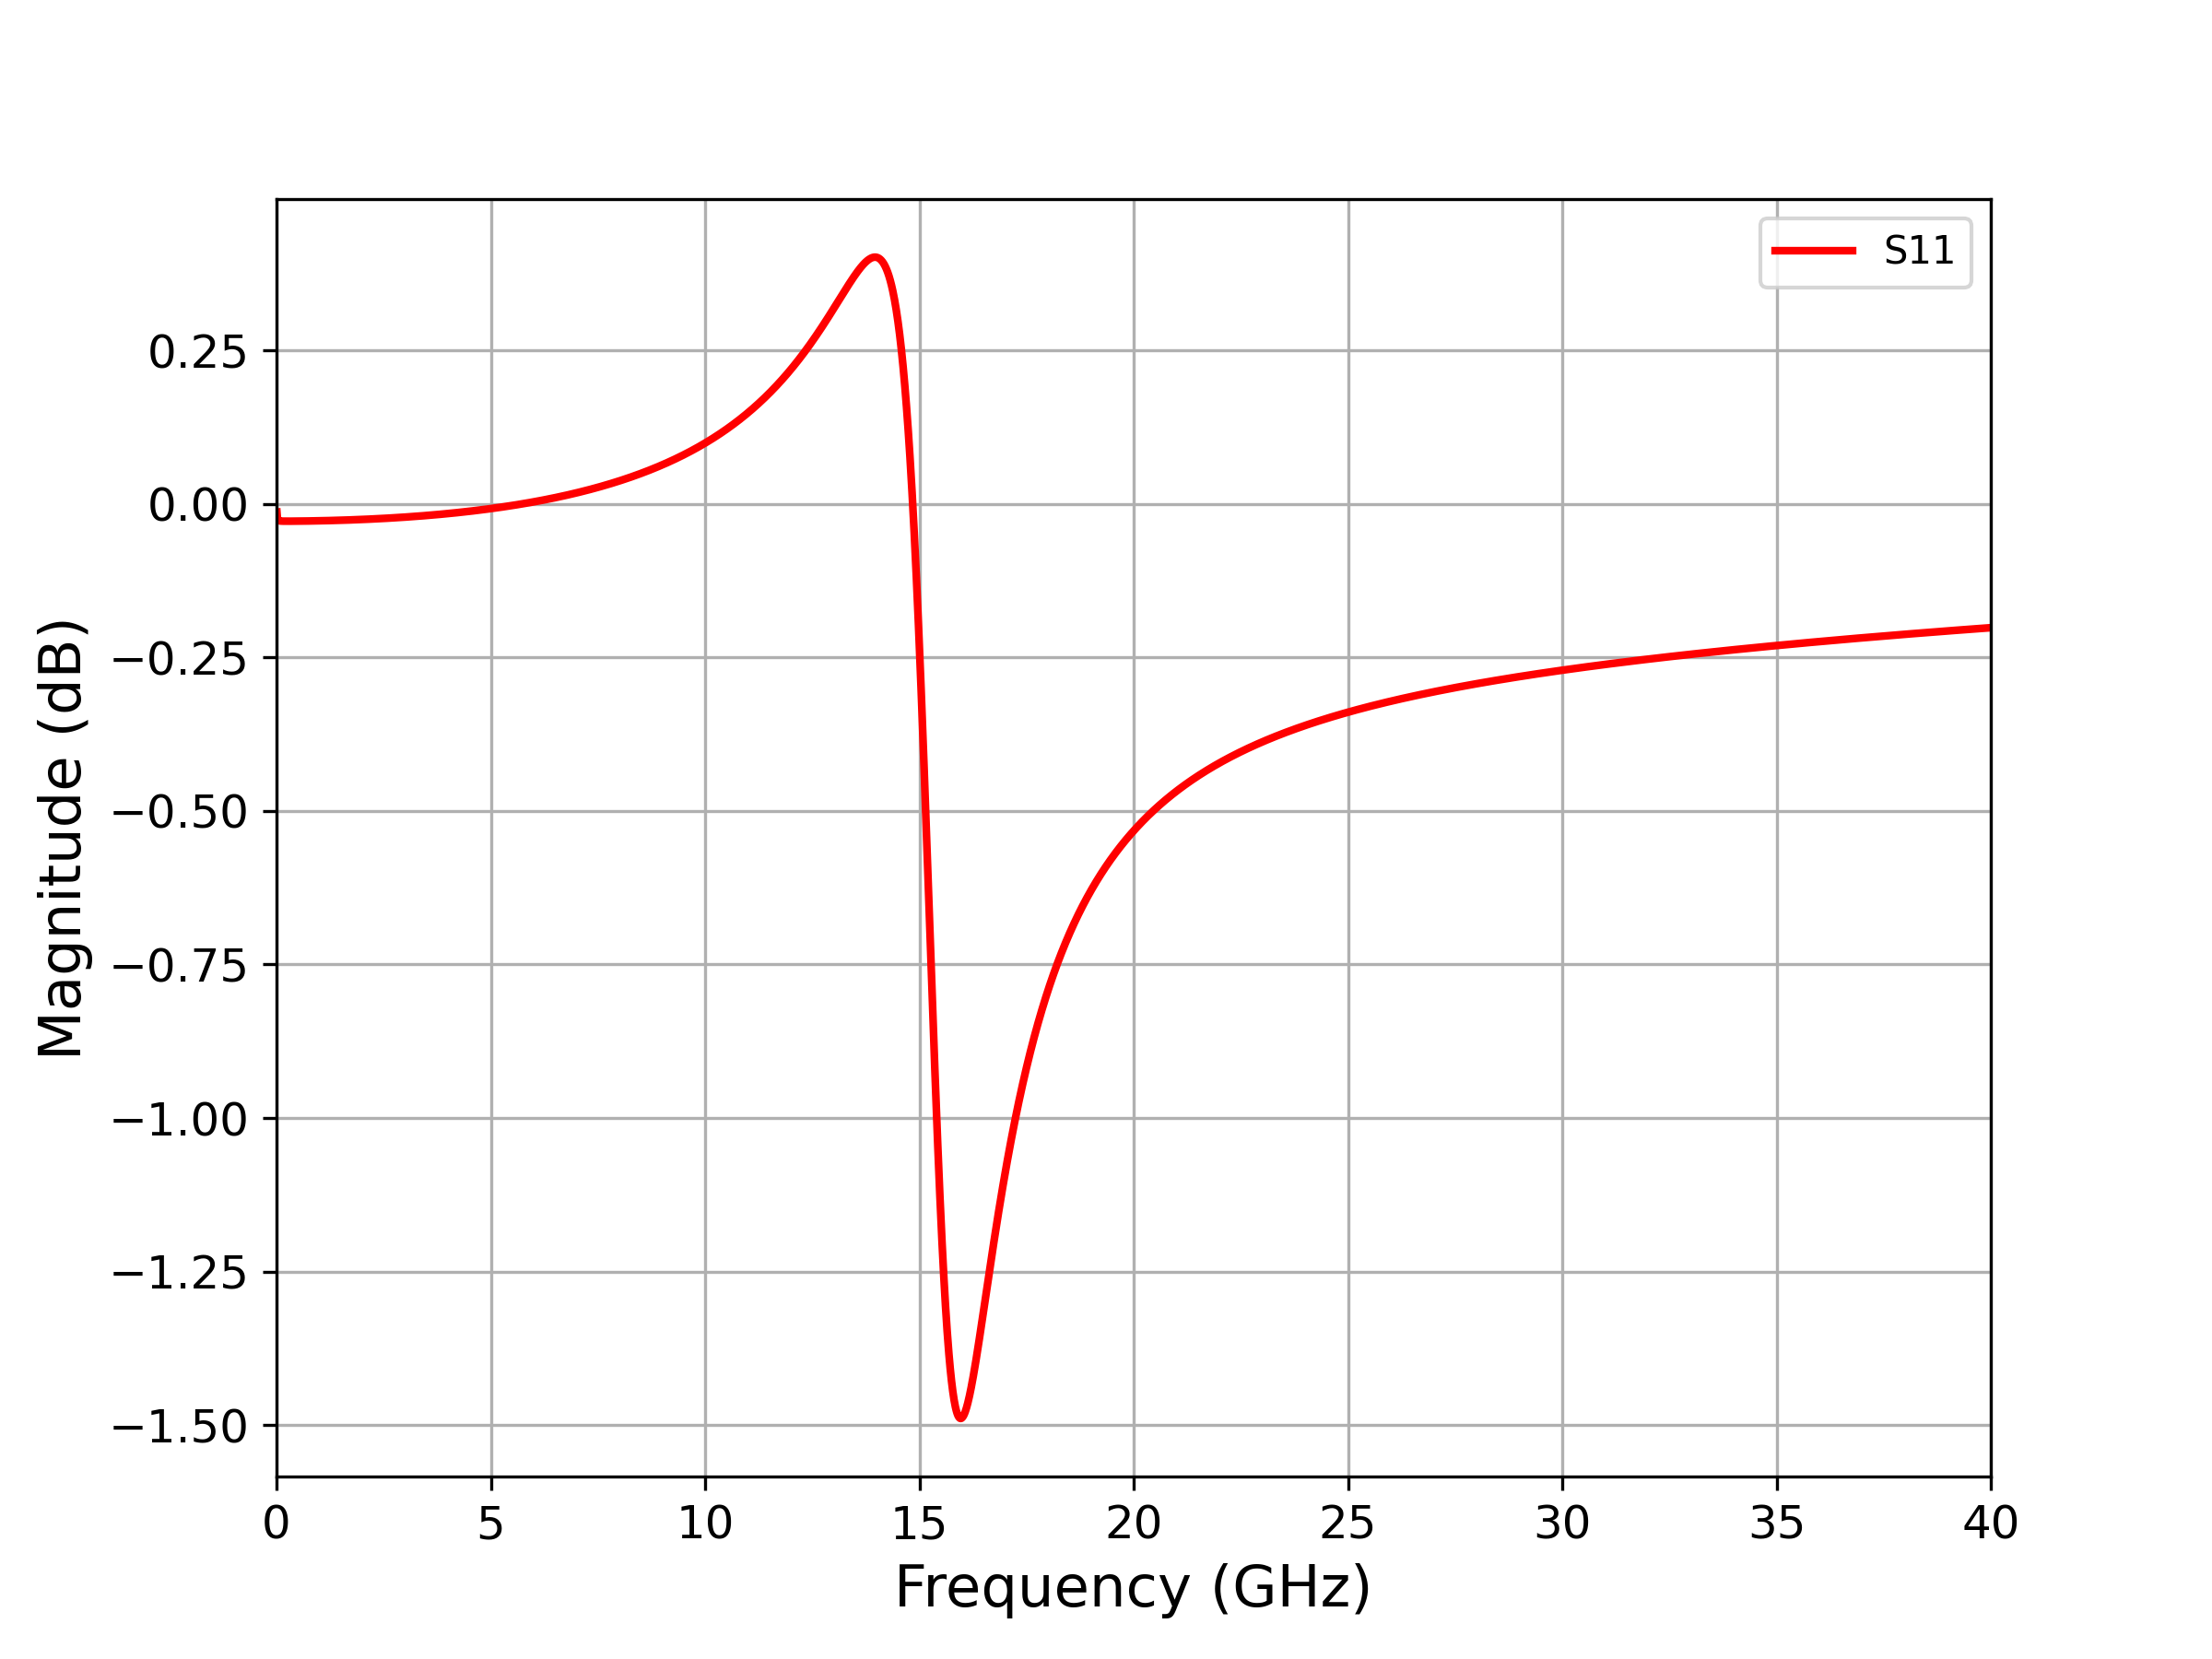
\includegraphics[]{figures/two_stage_s11.png}
%     }
%     \caption{$S_{11}$ parameter of a two-stage power amplifier (shown in Figure \ref{fig:double-stage-power-amplifier}) without matching network. The $S_{11}$ parameter is plotted from 0 GHz to 60 GHz.}
%     \label{fig:two-stage-without-cadence-s11}
% \end{figure}
% \begin{figure}[H]
%     \centering
%     \resizebox{0.8\textwidth}{!}{
%     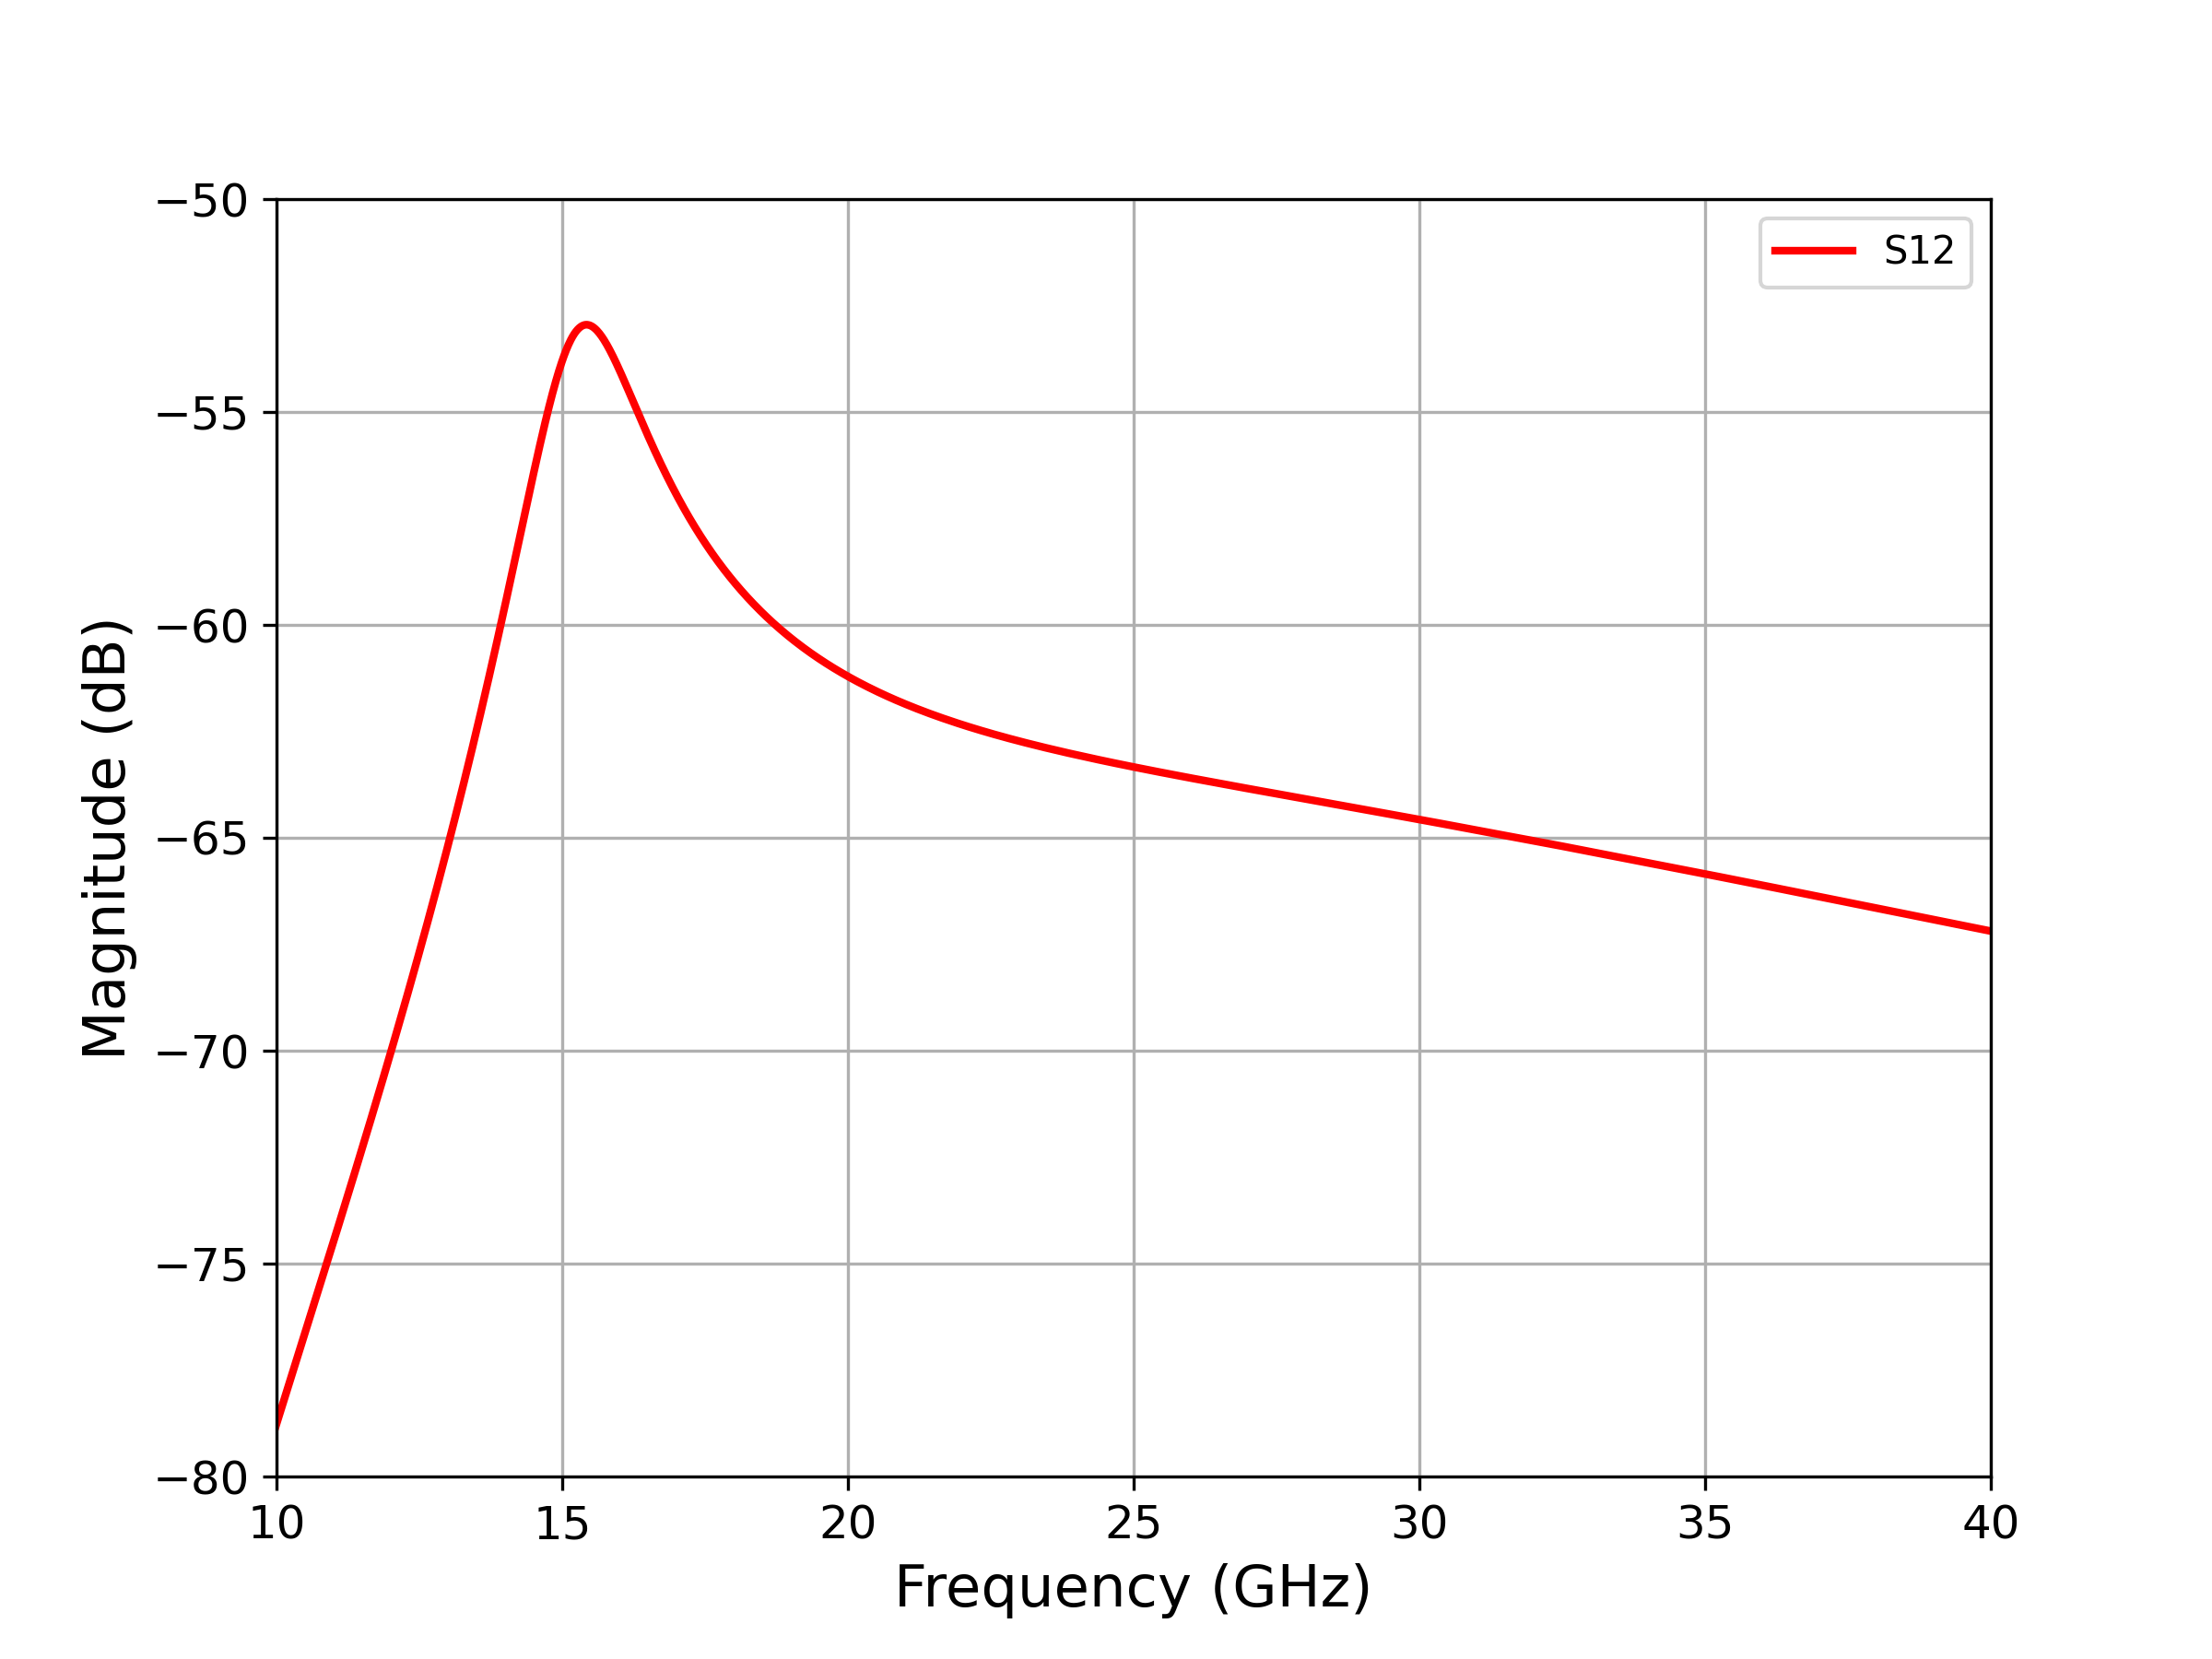
\includegraphics[]{figures/two_stage_s12.png}
%     }
%     \caption{$S_{12}$ parameter of a two-stage power amplifier (shown in Figure \ref{fig:double-stage-power-amplifier}) without matching network. The $S_{12}$ parameter is plotted from 0 GHz to 60 GHz.}
%     \label{fig:two-stage-without-cadence-s12}
% \end{figure}

\begin{figure}[H]
  \centering
  \begin{subfigure}{0.49\textwidth}
    \centering
    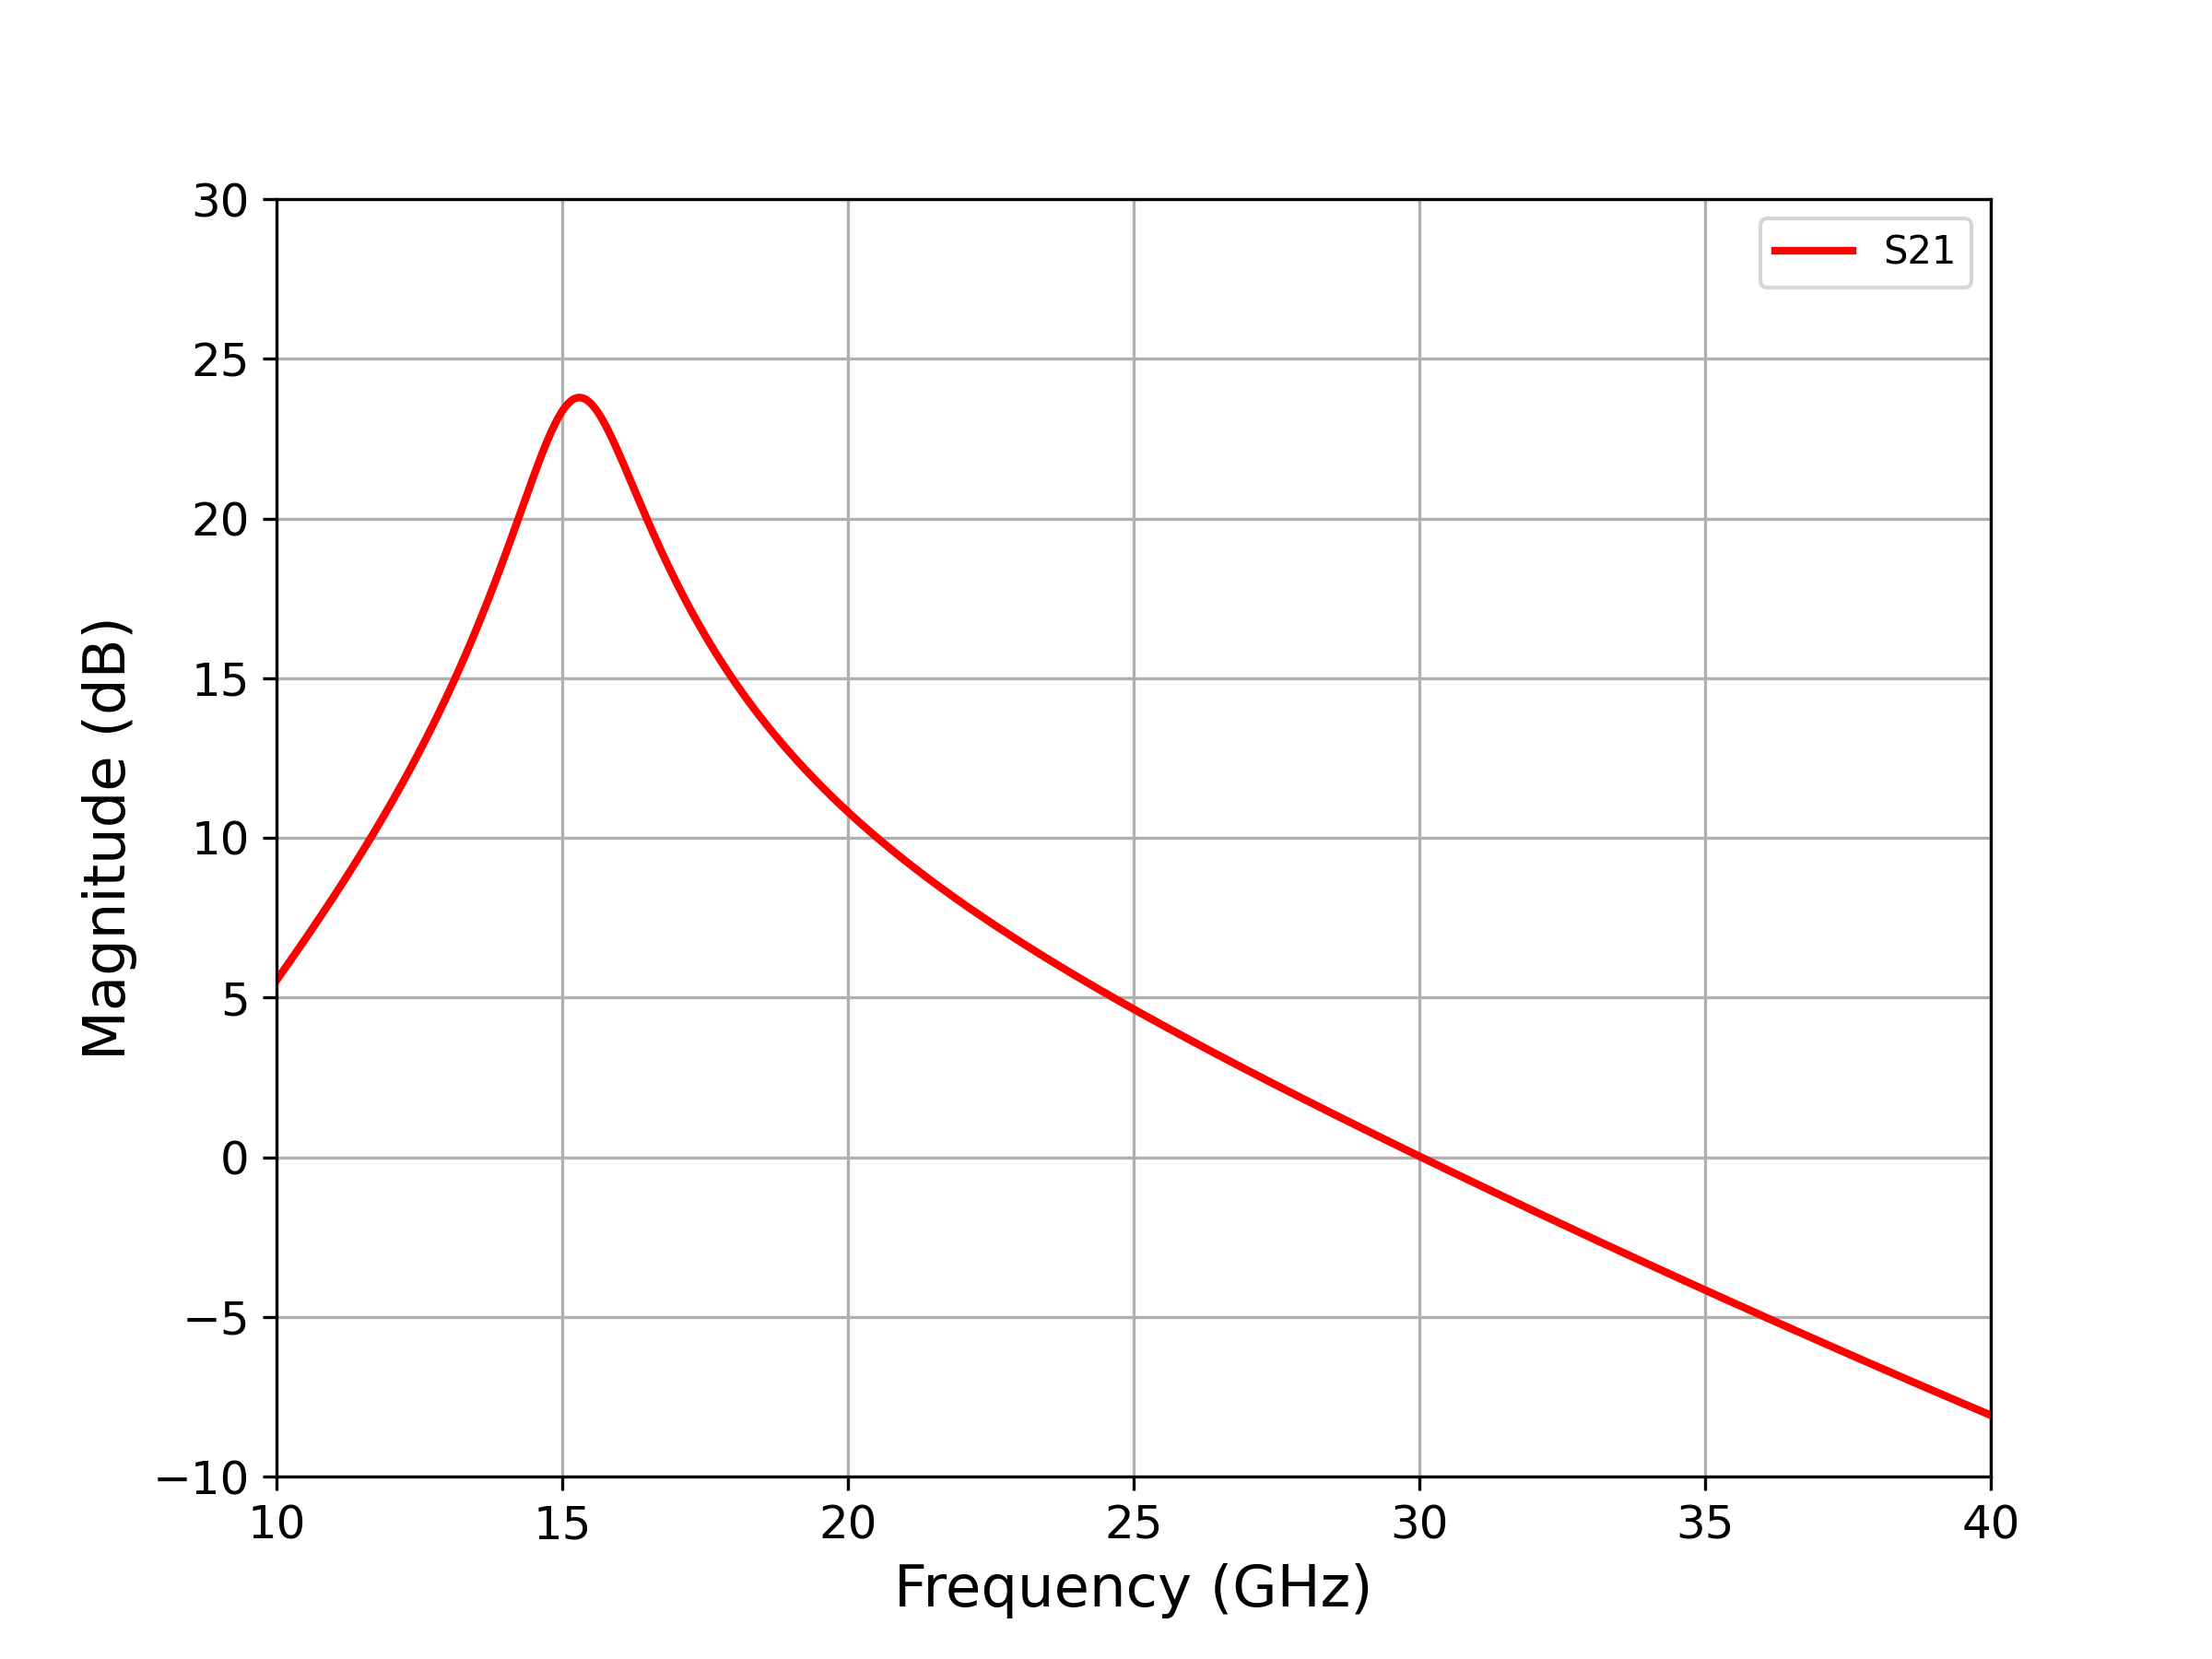
\includegraphics[width=\linewidth]{figures/two_stage_s21.png}
    \caption{}
    \label{fig:two-stage-without-cadence-s21}
  \end{subfigure}
  \hfill
  \begin{subfigure}{0.49\textwidth}
    \centering
    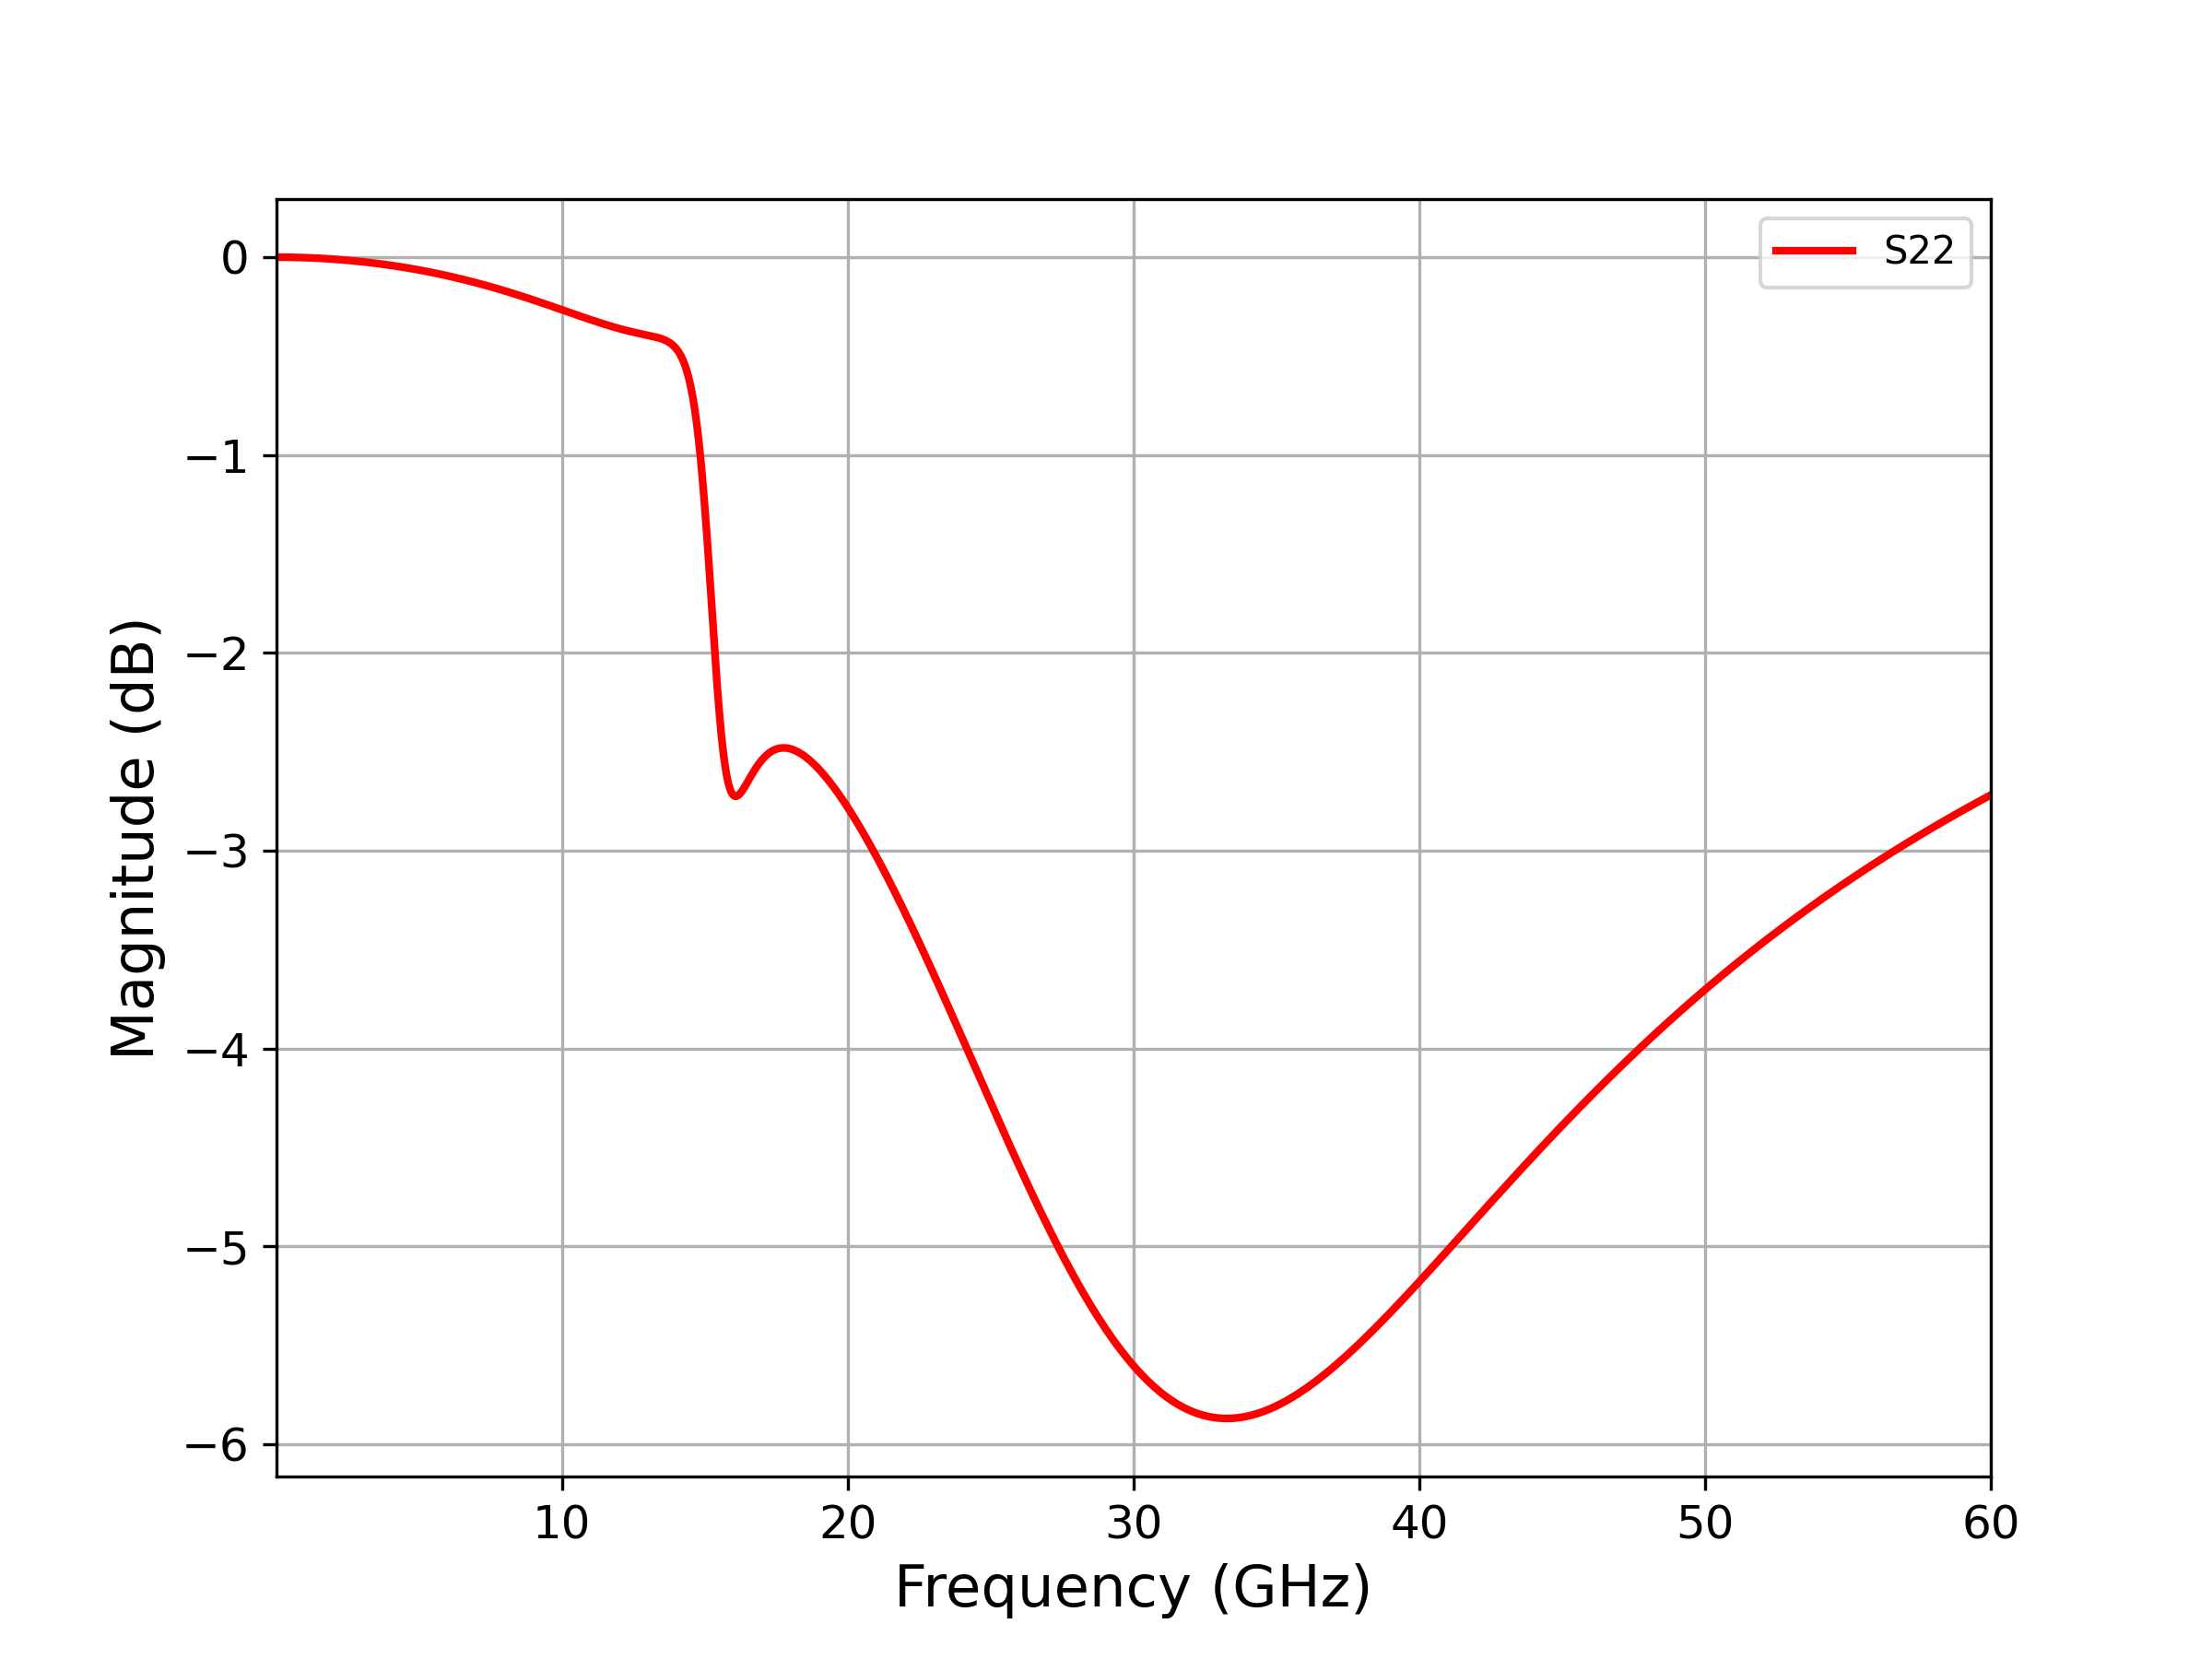
\includegraphics[width=\linewidth]{figures/two_stage_s22.png}
    \caption{}
     \label{fig:two-stage-without-cadence-s22}
  \end{subfigure}
  \caption{(a) $S_{21}$ parameter of a two-stage power amplifier (shown in Figure \ref{fig:double-stage-power-amplifier}) without matching network. (b) $S_{22}$ parameter of a two-stage power amplifier (shown in Figure \ref{fig:double-stage-power-amplifier}) without matching network.}
  \label{fig:two-stage-without-cadence-s21-s22}
\end{figure}

The maximum value of $S_{21}$ of a two-stage power amplifier is 24 dB at 15 GHz, which indicates a significant enhancement compared to the single-stage amplifier. However, the gain decreases drastically as the frequency increases, which limits the bandwidth, and the value of $S_{22}$ is less than -3 dB through 20 GHz to 50 GHz.
% \begin{figure}[H]
%     \centering
%     \resizebox{0.8\textwidth}{!}{
%     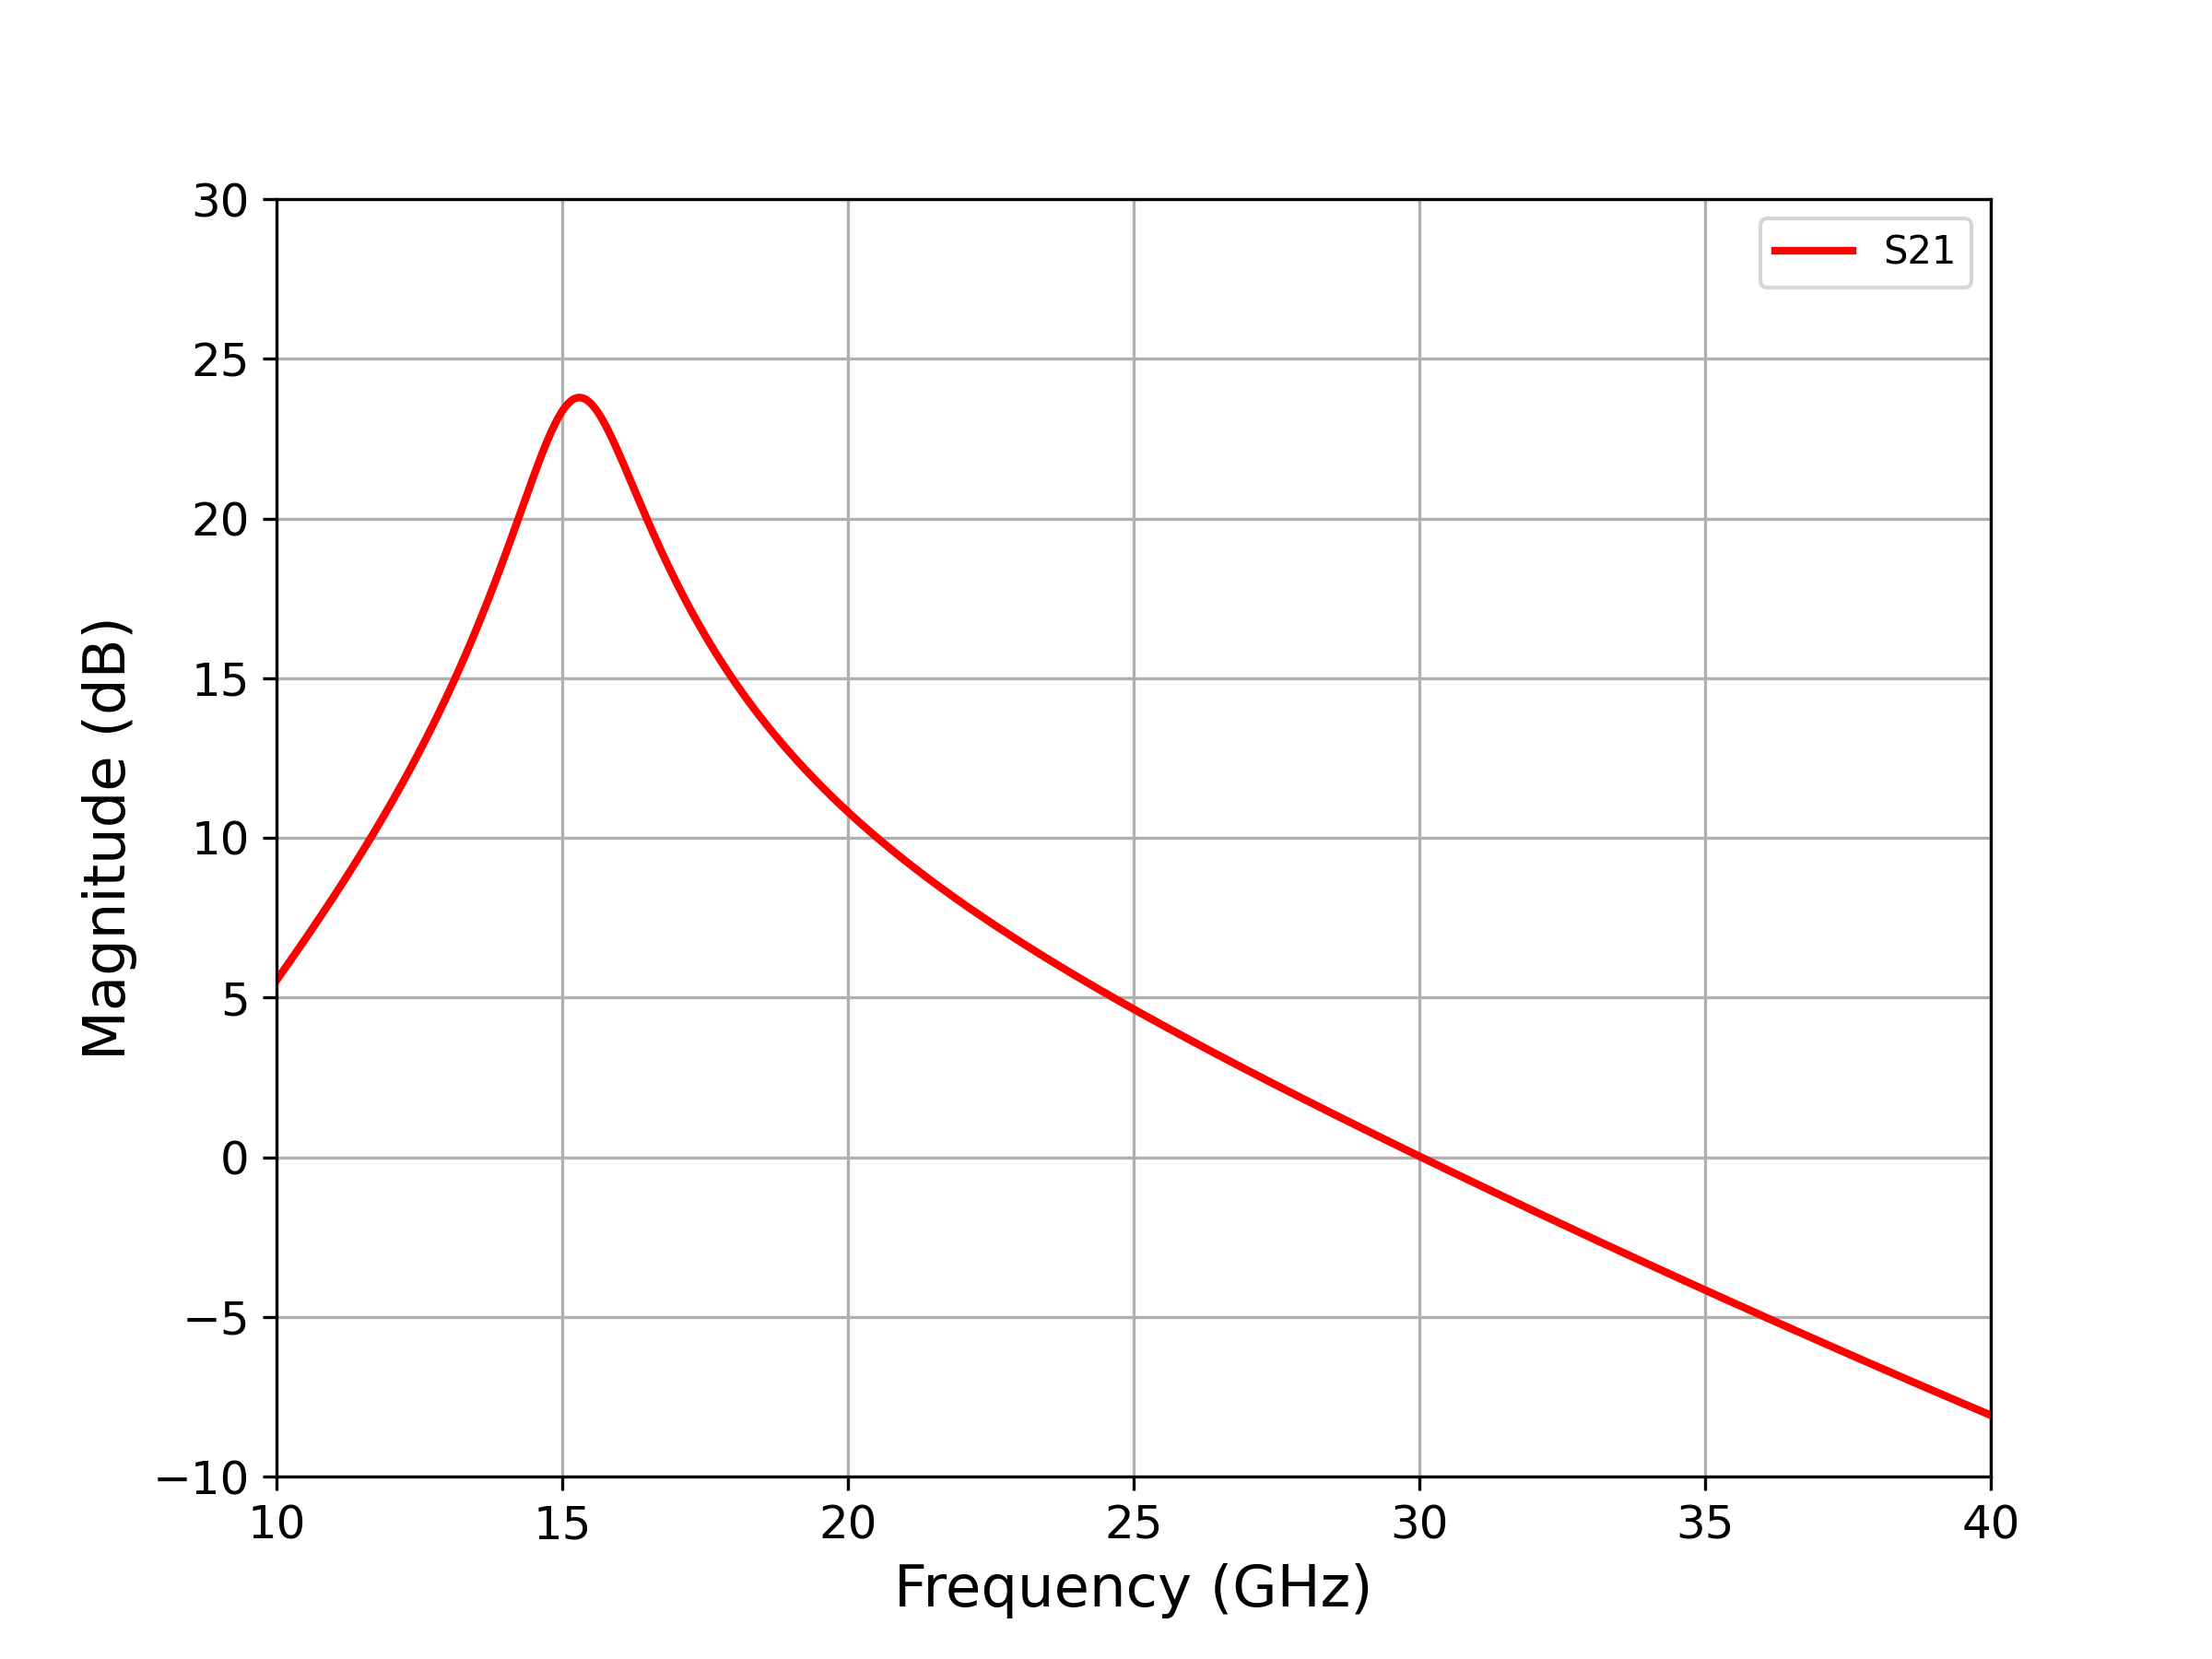
\includegraphics[]{figures/two_stage_s21.png}
%     }
%     \caption{$S_{21}$ parameter of a two-stage power amplifier (shown in Figure \ref{fig:double-stage-power-amplifier}) without matching network. The $S_{21}$ parameter is plotted from 0 GHz to 60 GHz.}
%     \label{fig:two-stage-without-cadence-s21}
% \end{figure}
% \begin{figure}[H]
%     \centering
%     \resizebox{0.8\textwidth}{!}{
%     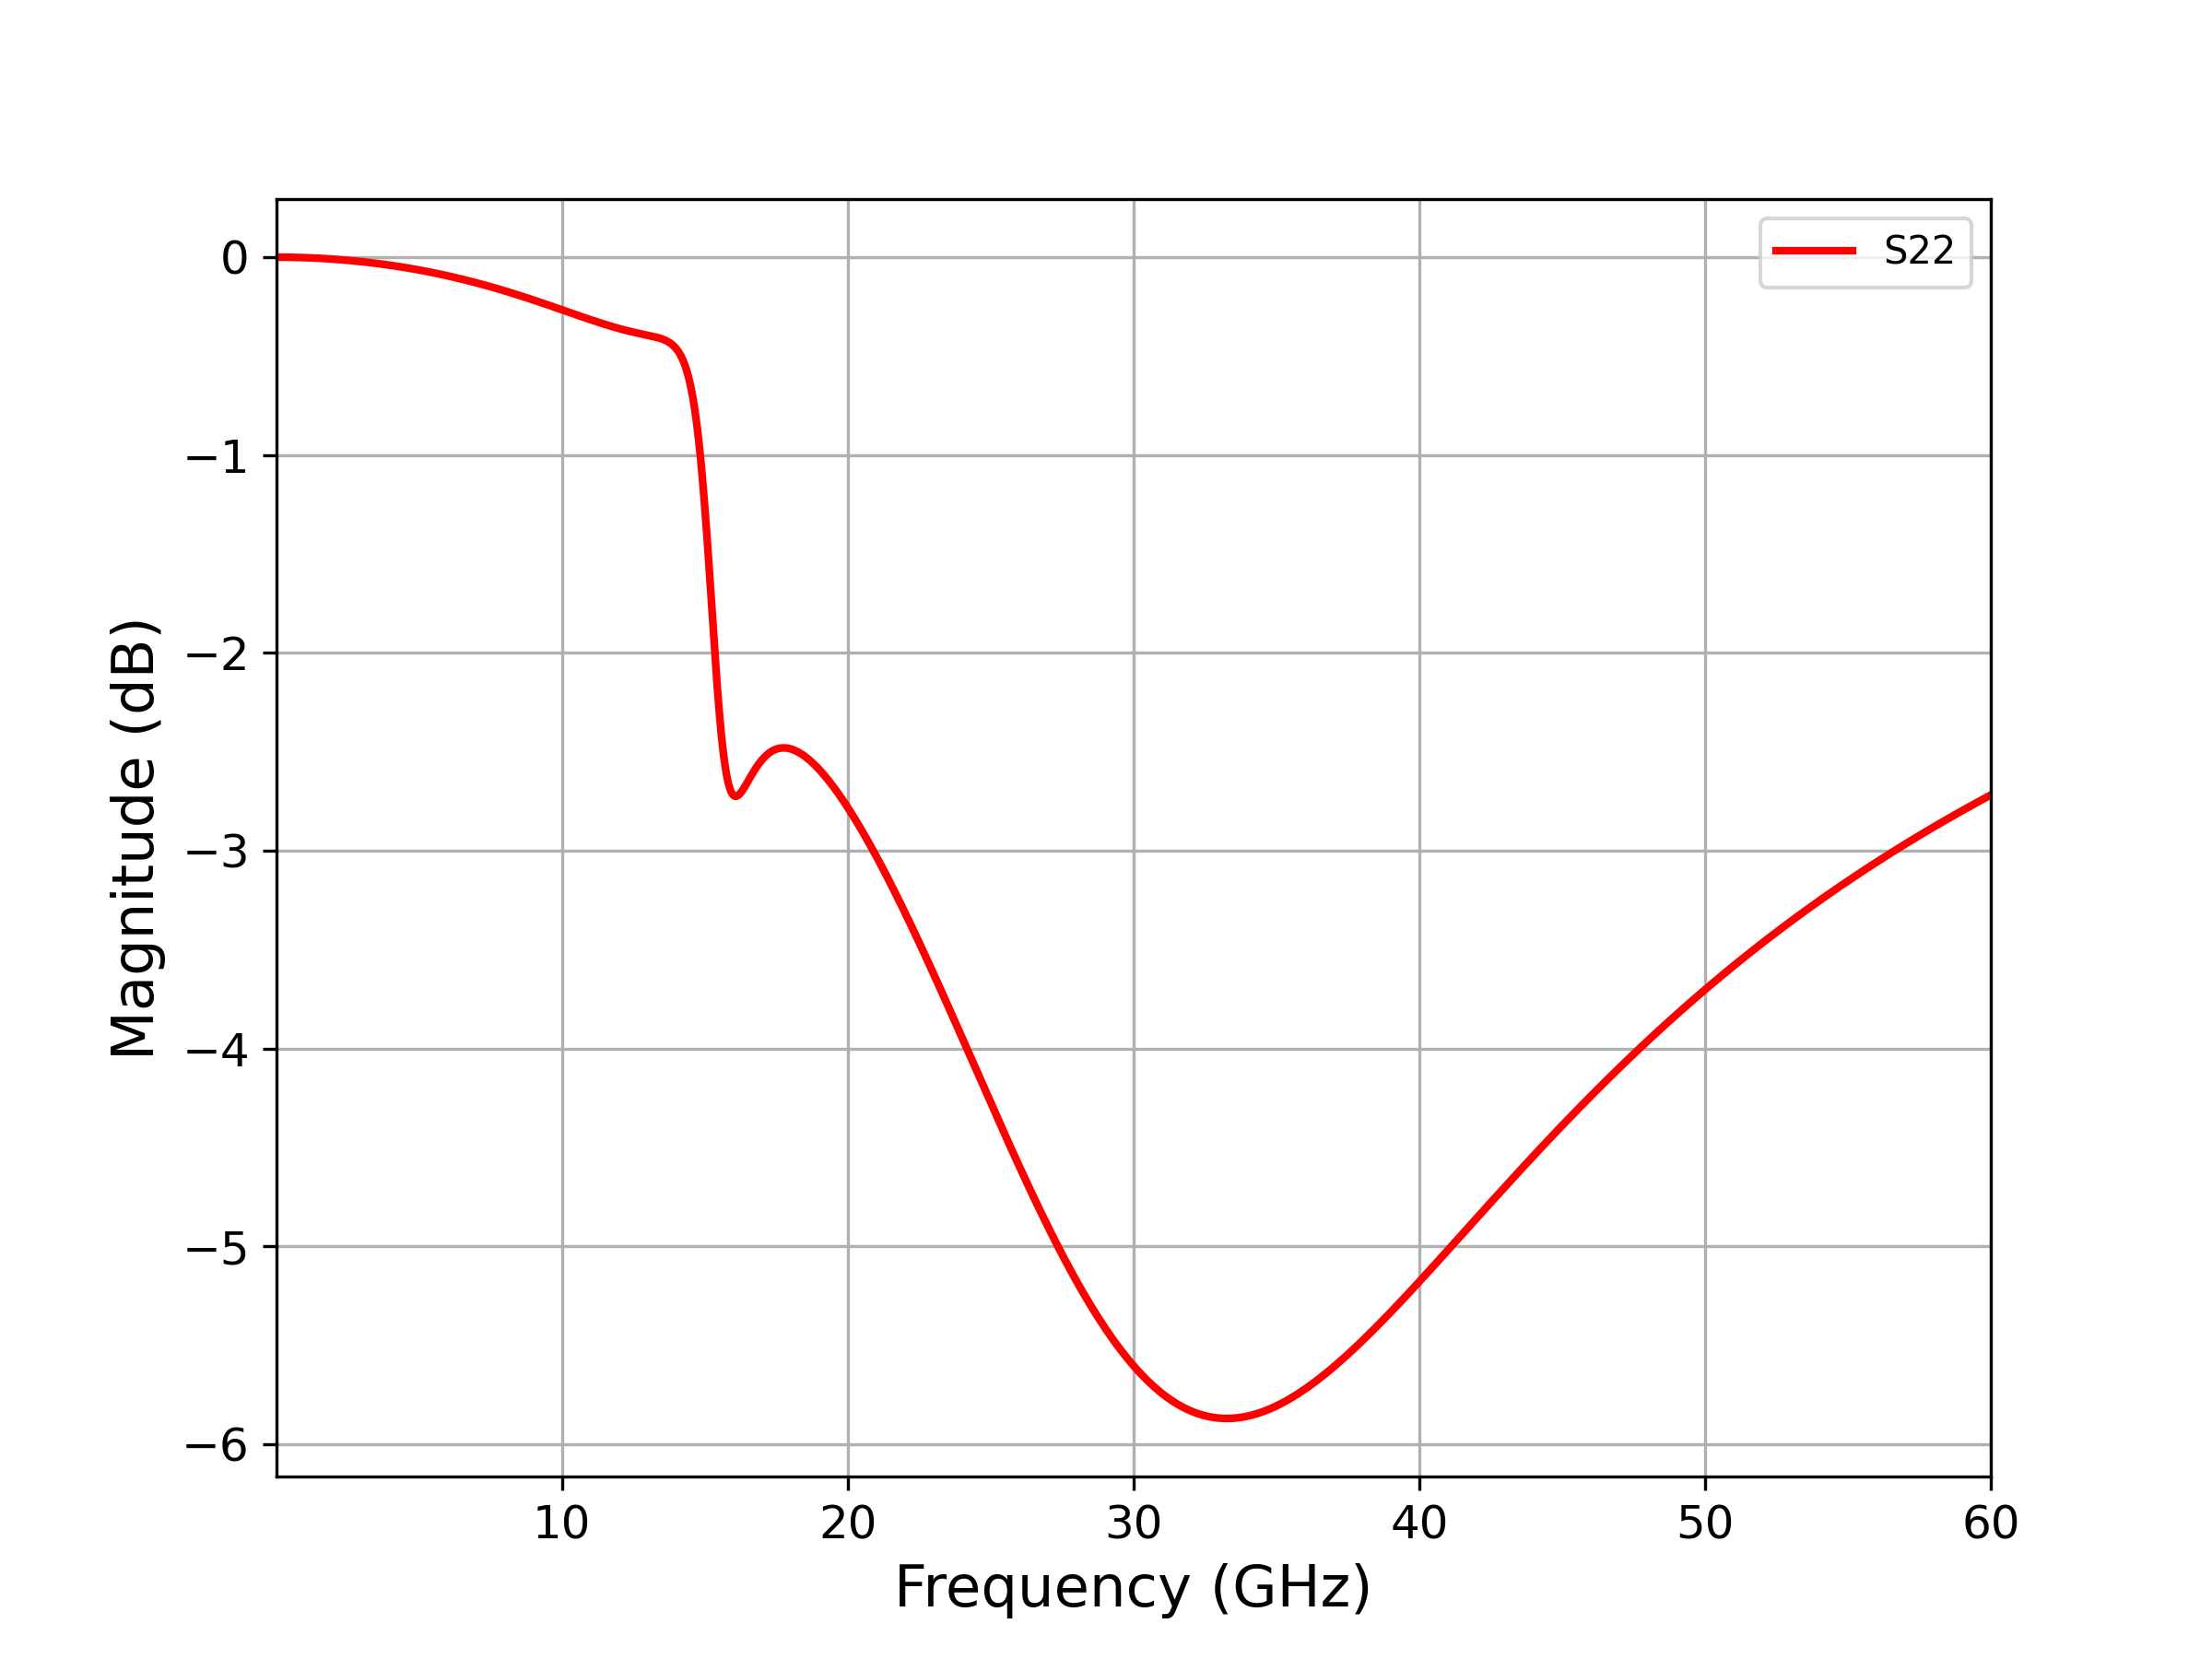
\includegraphics[]{figures/two_stage_s22.png}
%     }
%     \caption{$S_{22}$ parameter of a two-stage power amplifier (shown in Figure \ref{fig:double-stage-power-amplifier}) without matching network. The $S_{22}$ parameter is plotted from 0 GHz to 60 GHz.}
%     \label{fig:two-stage-without-cadence-s22}
% \end{figure}
%The $S$ parameter simulation of proposed two stage power amplifier(Figure \ref{fig:two-stage-with-input-interstage-matching}) with input and interstage matching network is shown below

\begin{figure}[H]
  \centering
  \begin{subfigure}{0.49\textwidth}
    \centering
    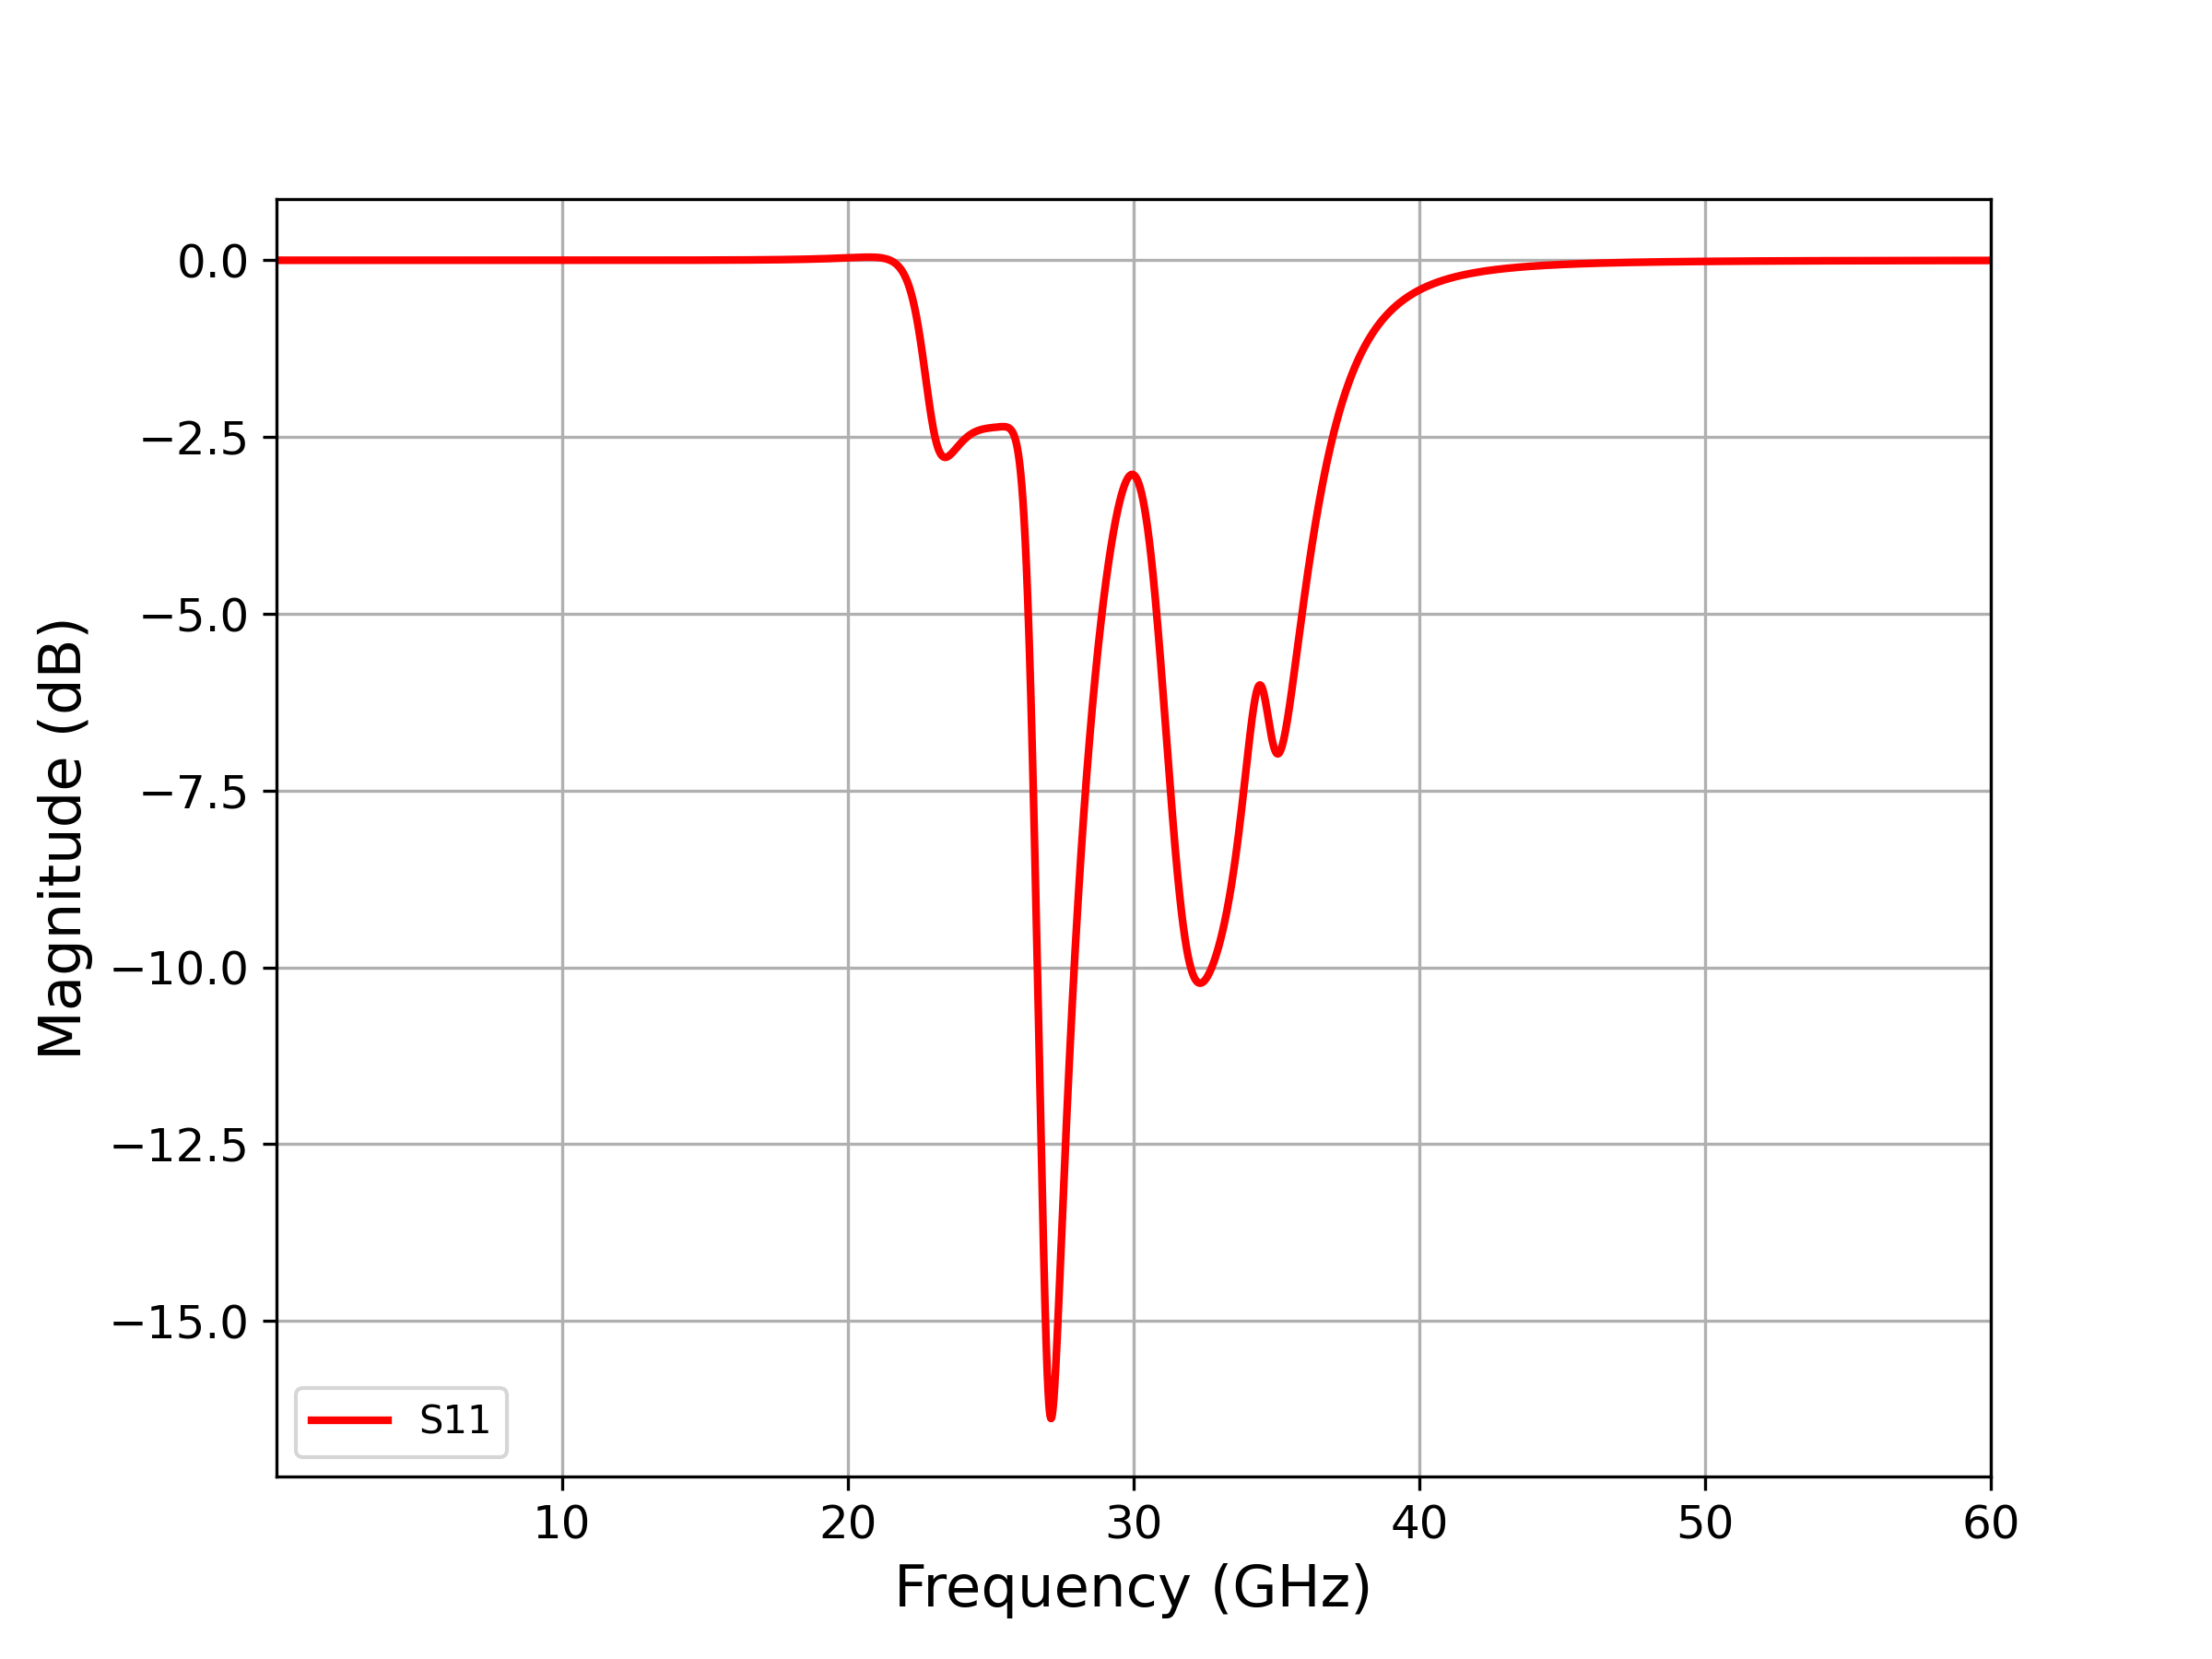
\includegraphics[width=\linewidth]{figures/two_stage_withMatching_s11.png}
    \caption{}
    \label{fig:two-stage-withmatching-cadence-s11}
  \end{subfigure}
  \hfill
  \begin{subfigure}{0.49\textwidth}
    \centering
    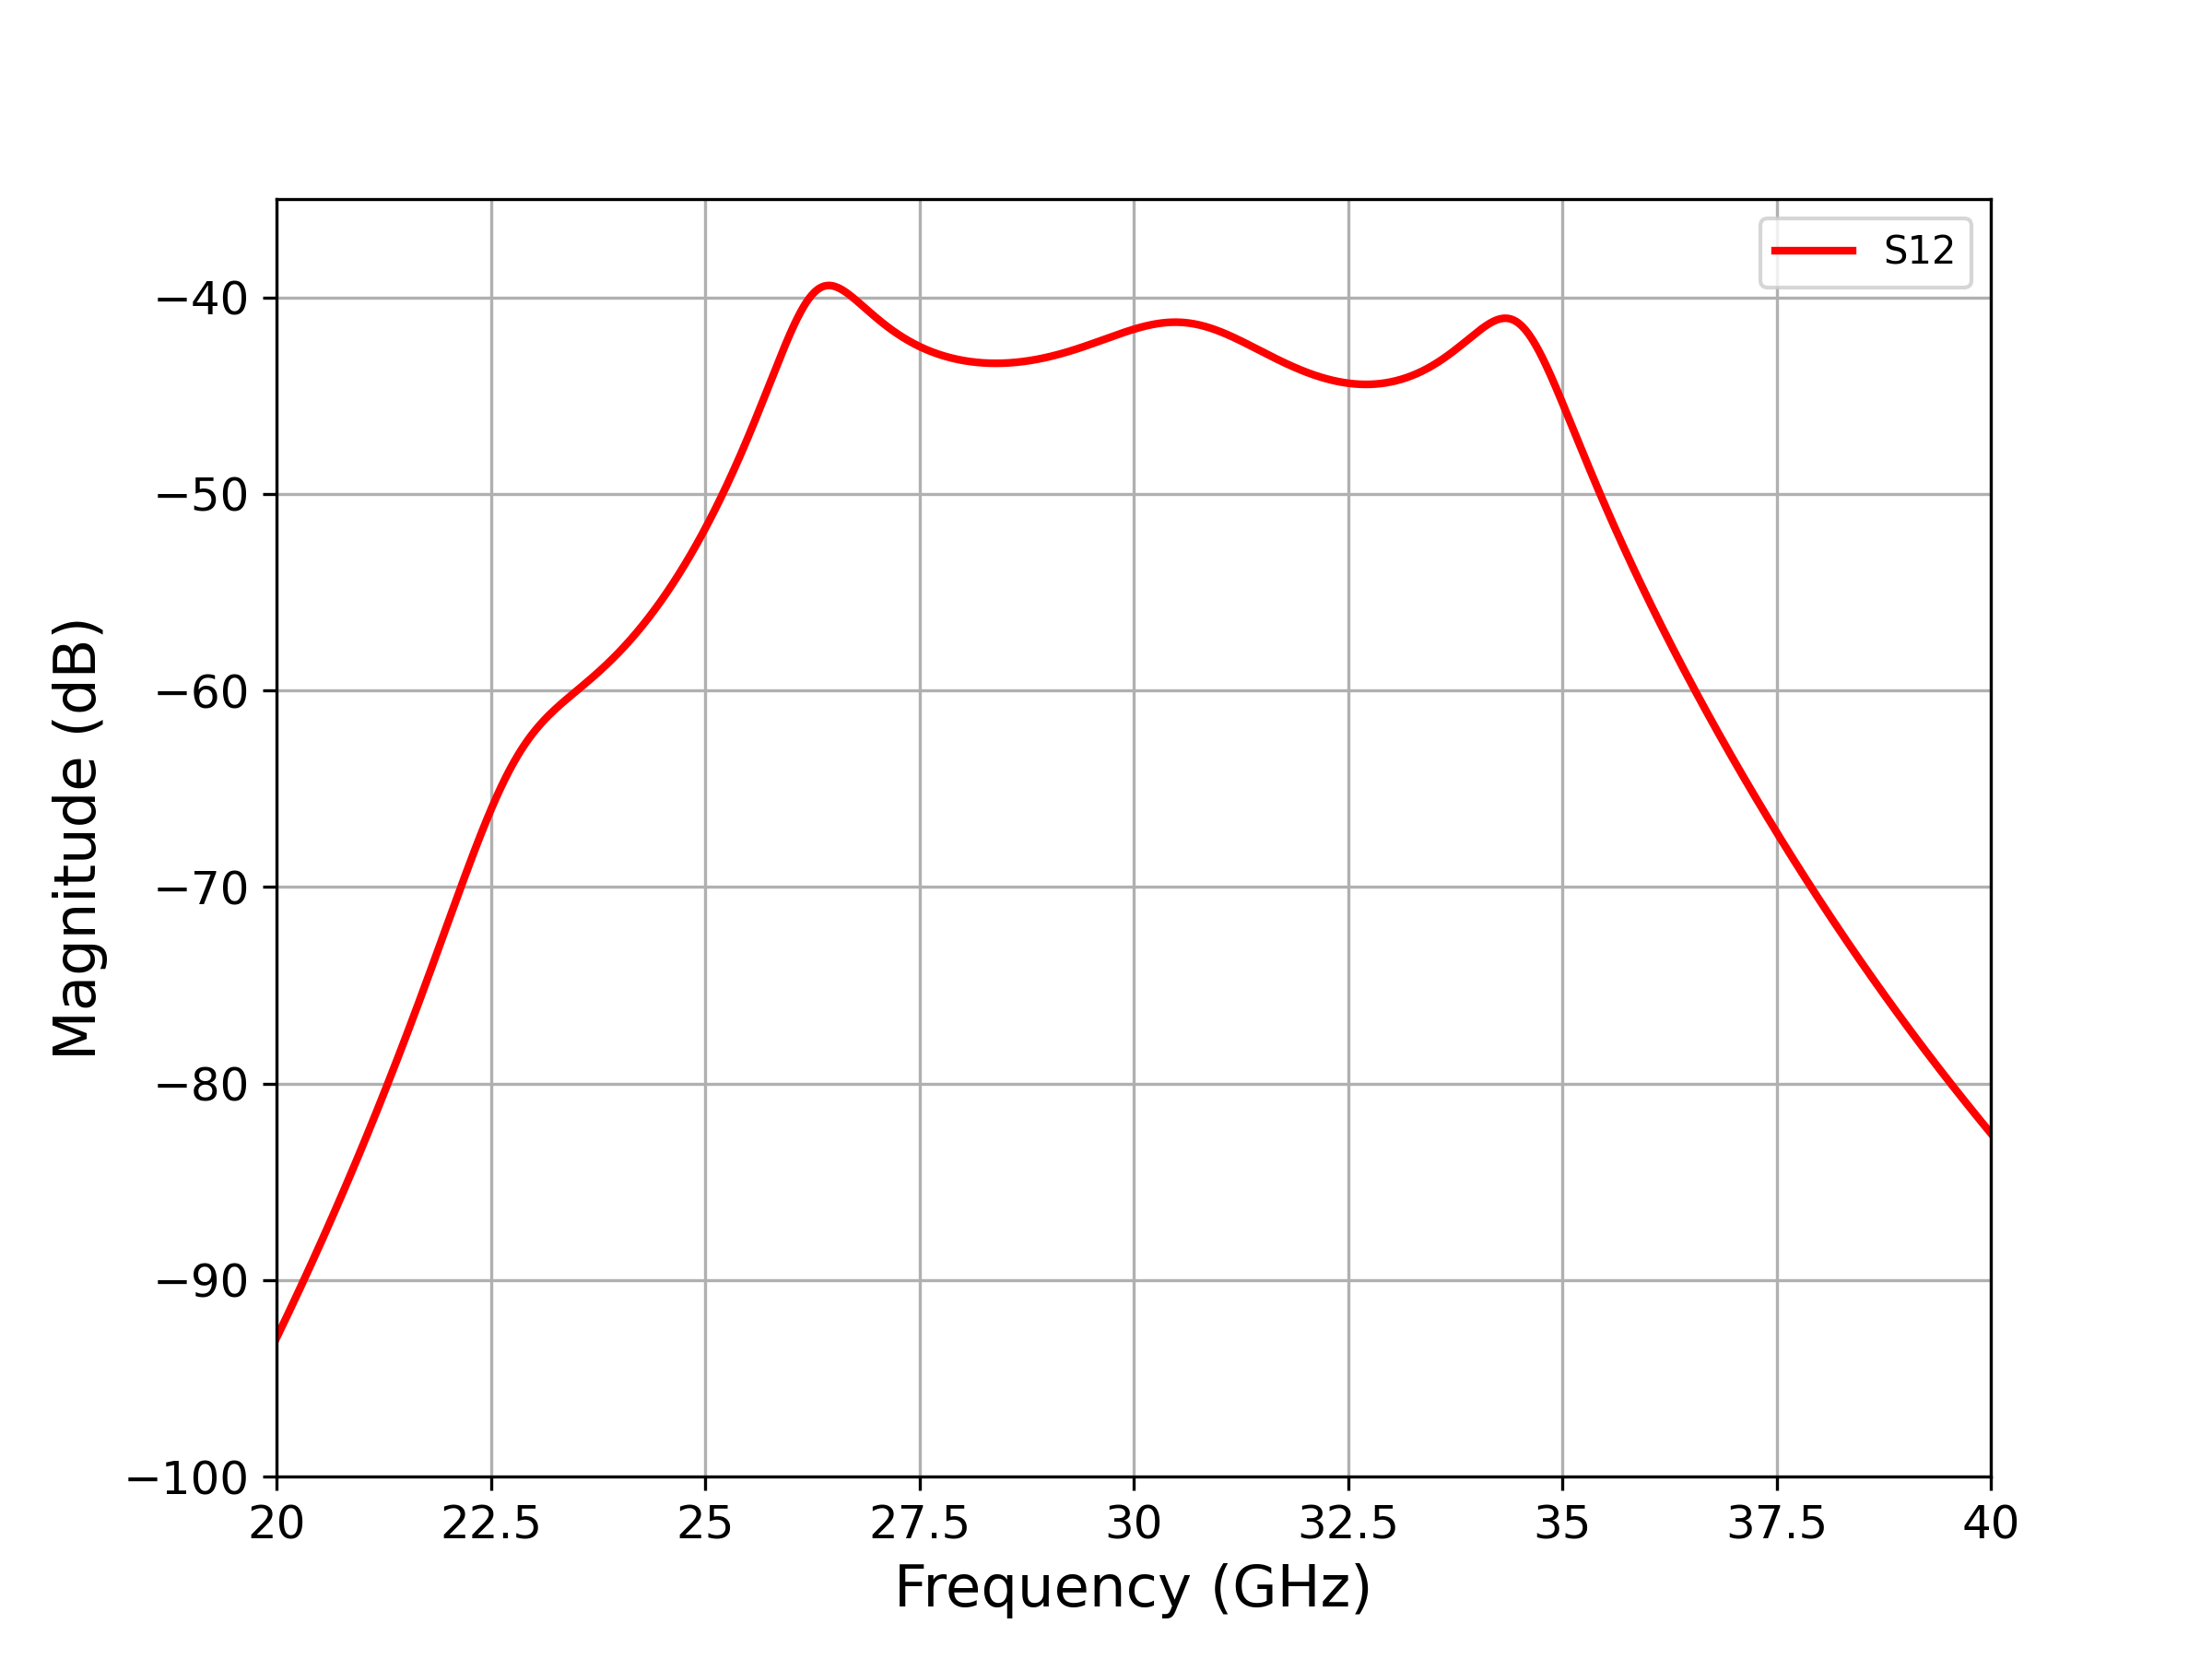
\includegraphics[width=\linewidth]{figures/two_stage_withMatching_s12.png}
    \caption{}
     \label{fig:two-stage-withmatching-cadence-s12}
  \end{subfigure}
  \caption{(a) $S_{11}$ parameter of a two-stage power amplifier (shown in Figure \ref{fig:two-stage-with-input-interstage-matching}) with input and interstage matching network. (b) $S_{12}$ parameter of a two-stage power amplifier (shown in Figure \ref{fig:two-stage-with-input-interstage-matching}) with input and interstage matching network.}
  \label{fig:two-stage-withmatching-cadence-s11-s12}
\end{figure}

To improve input impedance matching and inter-stage impedance matching, an input matching network is introduced at the input side of the proposed PA, and an inter-stage matching network is also introduced between the first and second stages of the proposed PA. The proposed PA network achieves better input matching with $S_{11}$ values of -16.38 dB at 27.12 GHz and -10.22 dB at 32.33 GHz. This indicates that a larger portion of the power is being absorbed by the amplifier rather than being reflected back. The proposed PA also exhibits good reverse isolation ($S_{12}$) of -40 dB over the frequency range of 25 to 35 GHz.

% \begin{figure}[H]
%     \centering
%     \resizebox{0.8\textwidth}{!}{
%     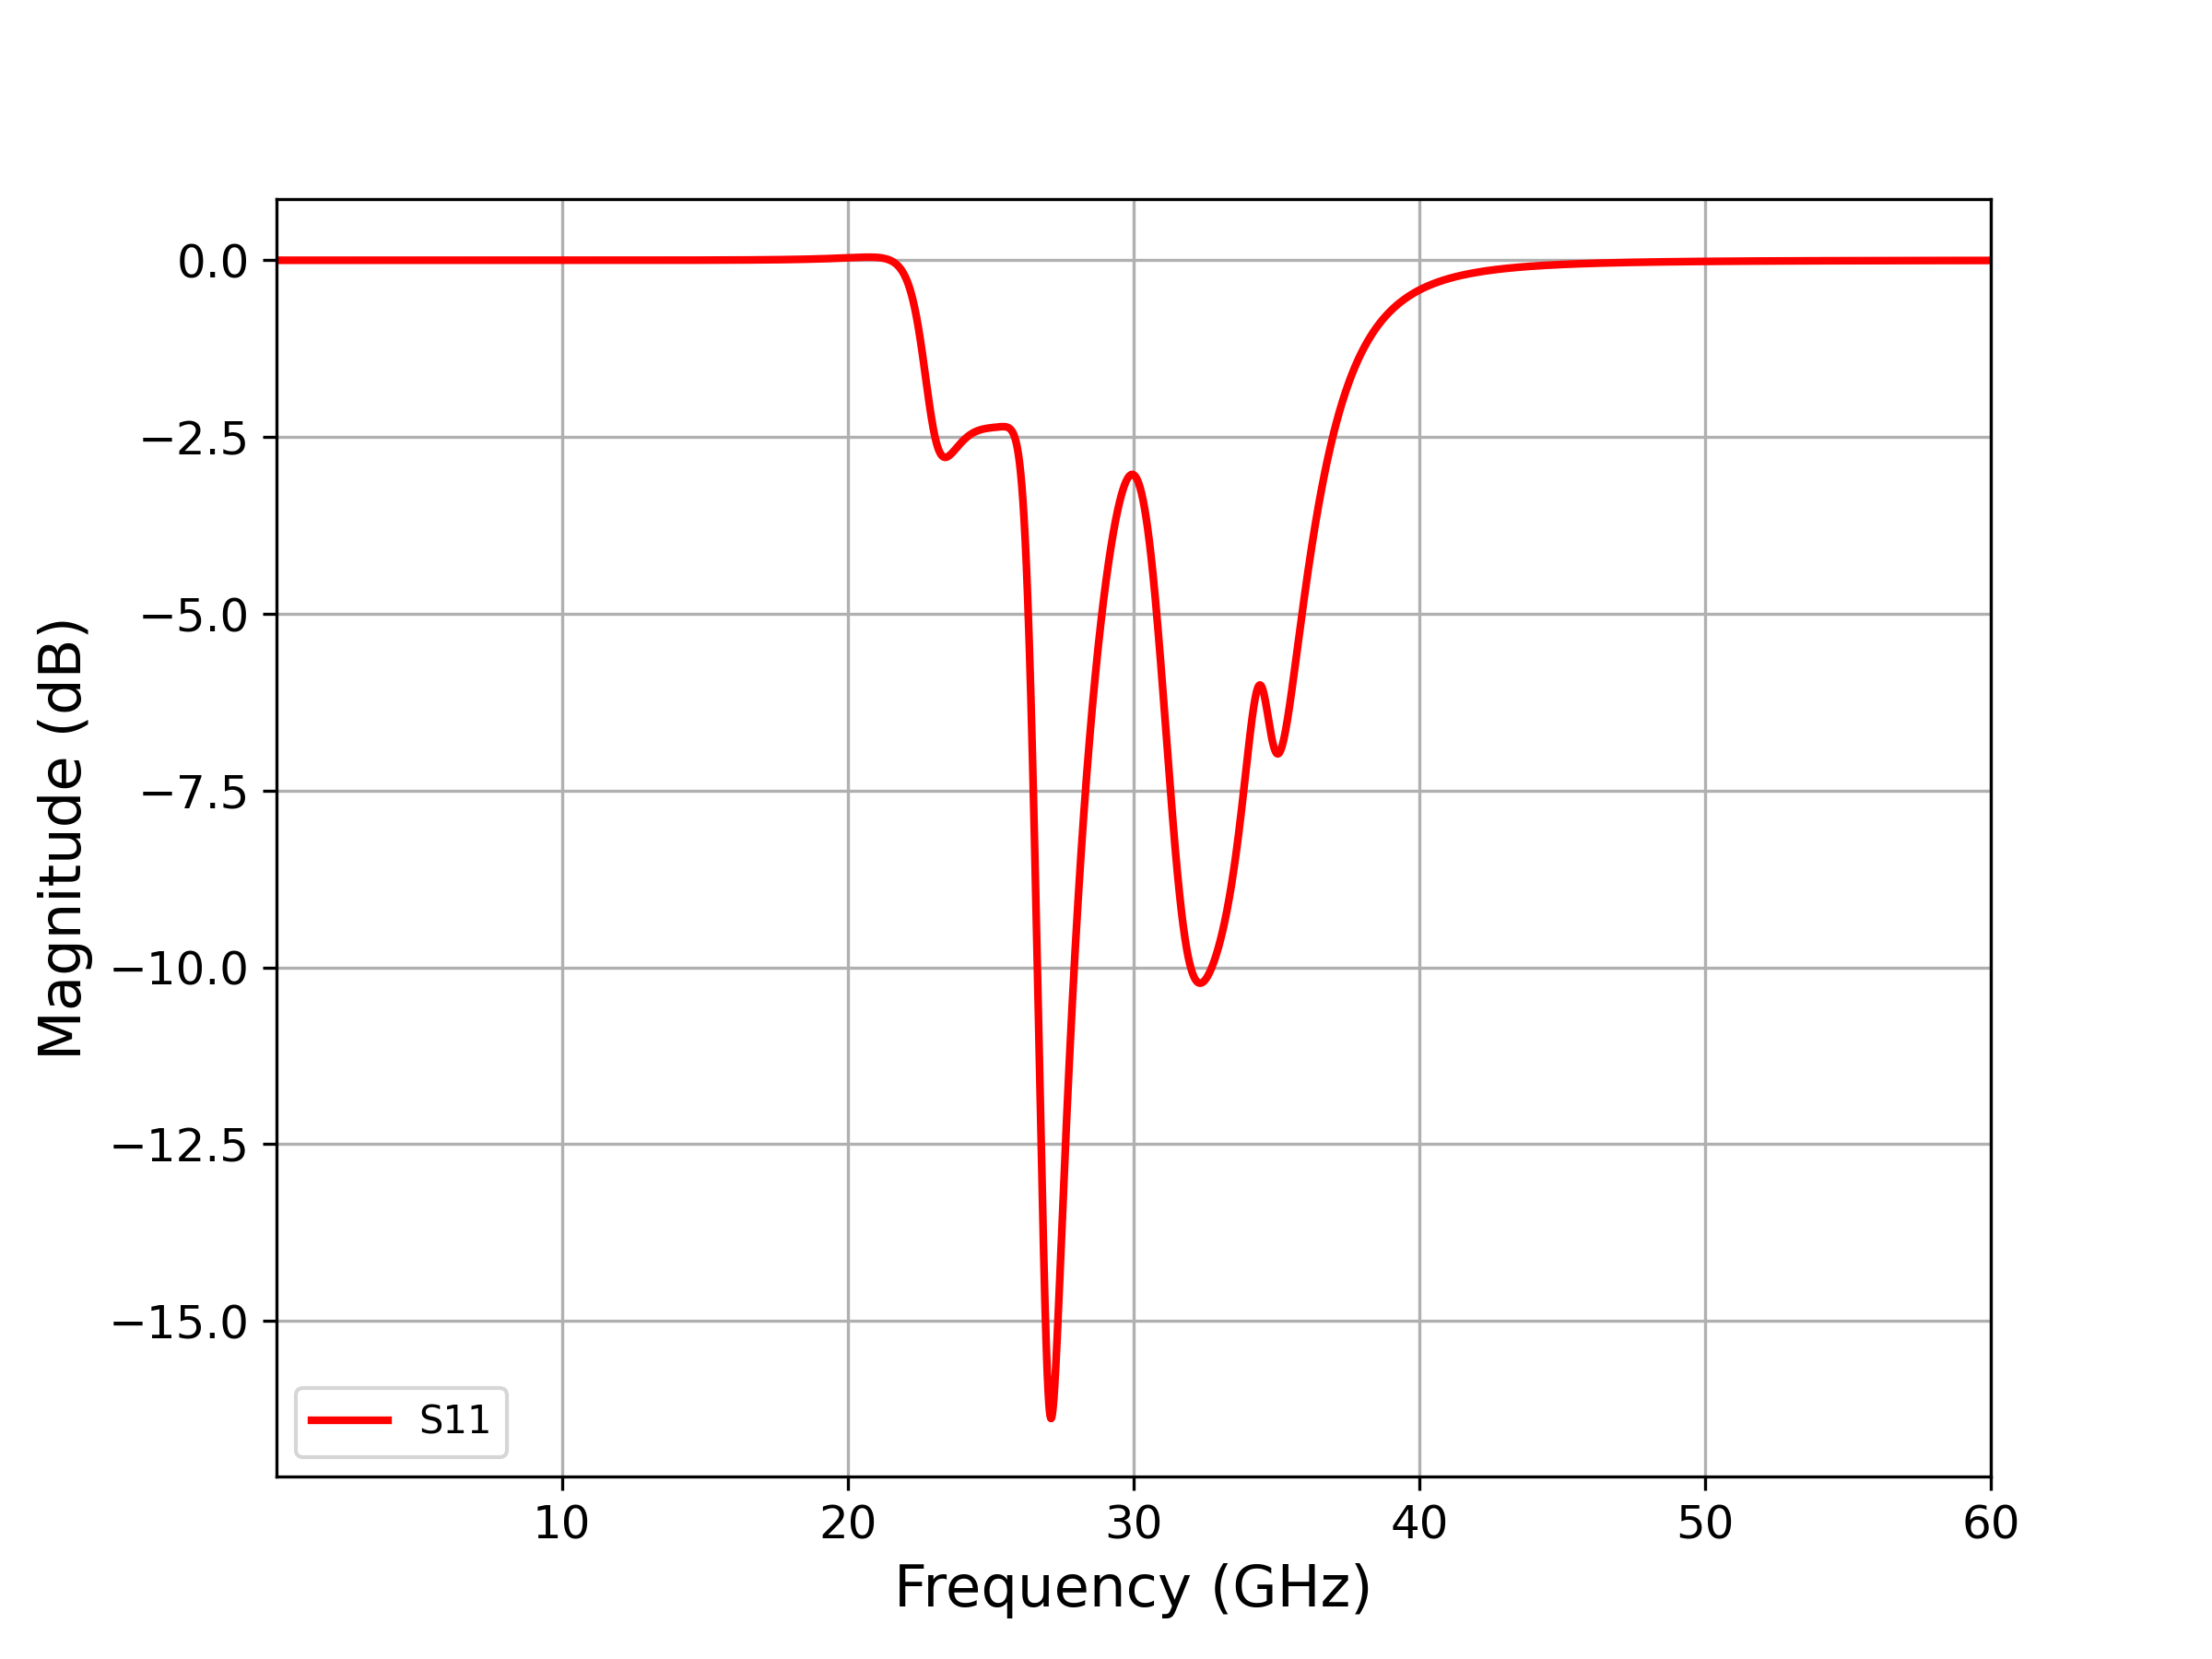
\includegraphics[]{figures/two_stage_withMatching_s11.png}
%     }
%     \caption{$S_{11}$ parameter of a two-stage power amplifier (shown in Figure \ref{fig:two-stage-with-input-interstage-matching}) with input and interstage matching network. The $S_{11}$ parameter is plotted from 0 GHz to 60 GHz.}
%     \label{fig:two-stage-withmatching-cadence-s11}
% \end{figure}
% \begin{figure}[H]
%     \centering
%     \resizebox{0.8\textwidth}{!}{
%     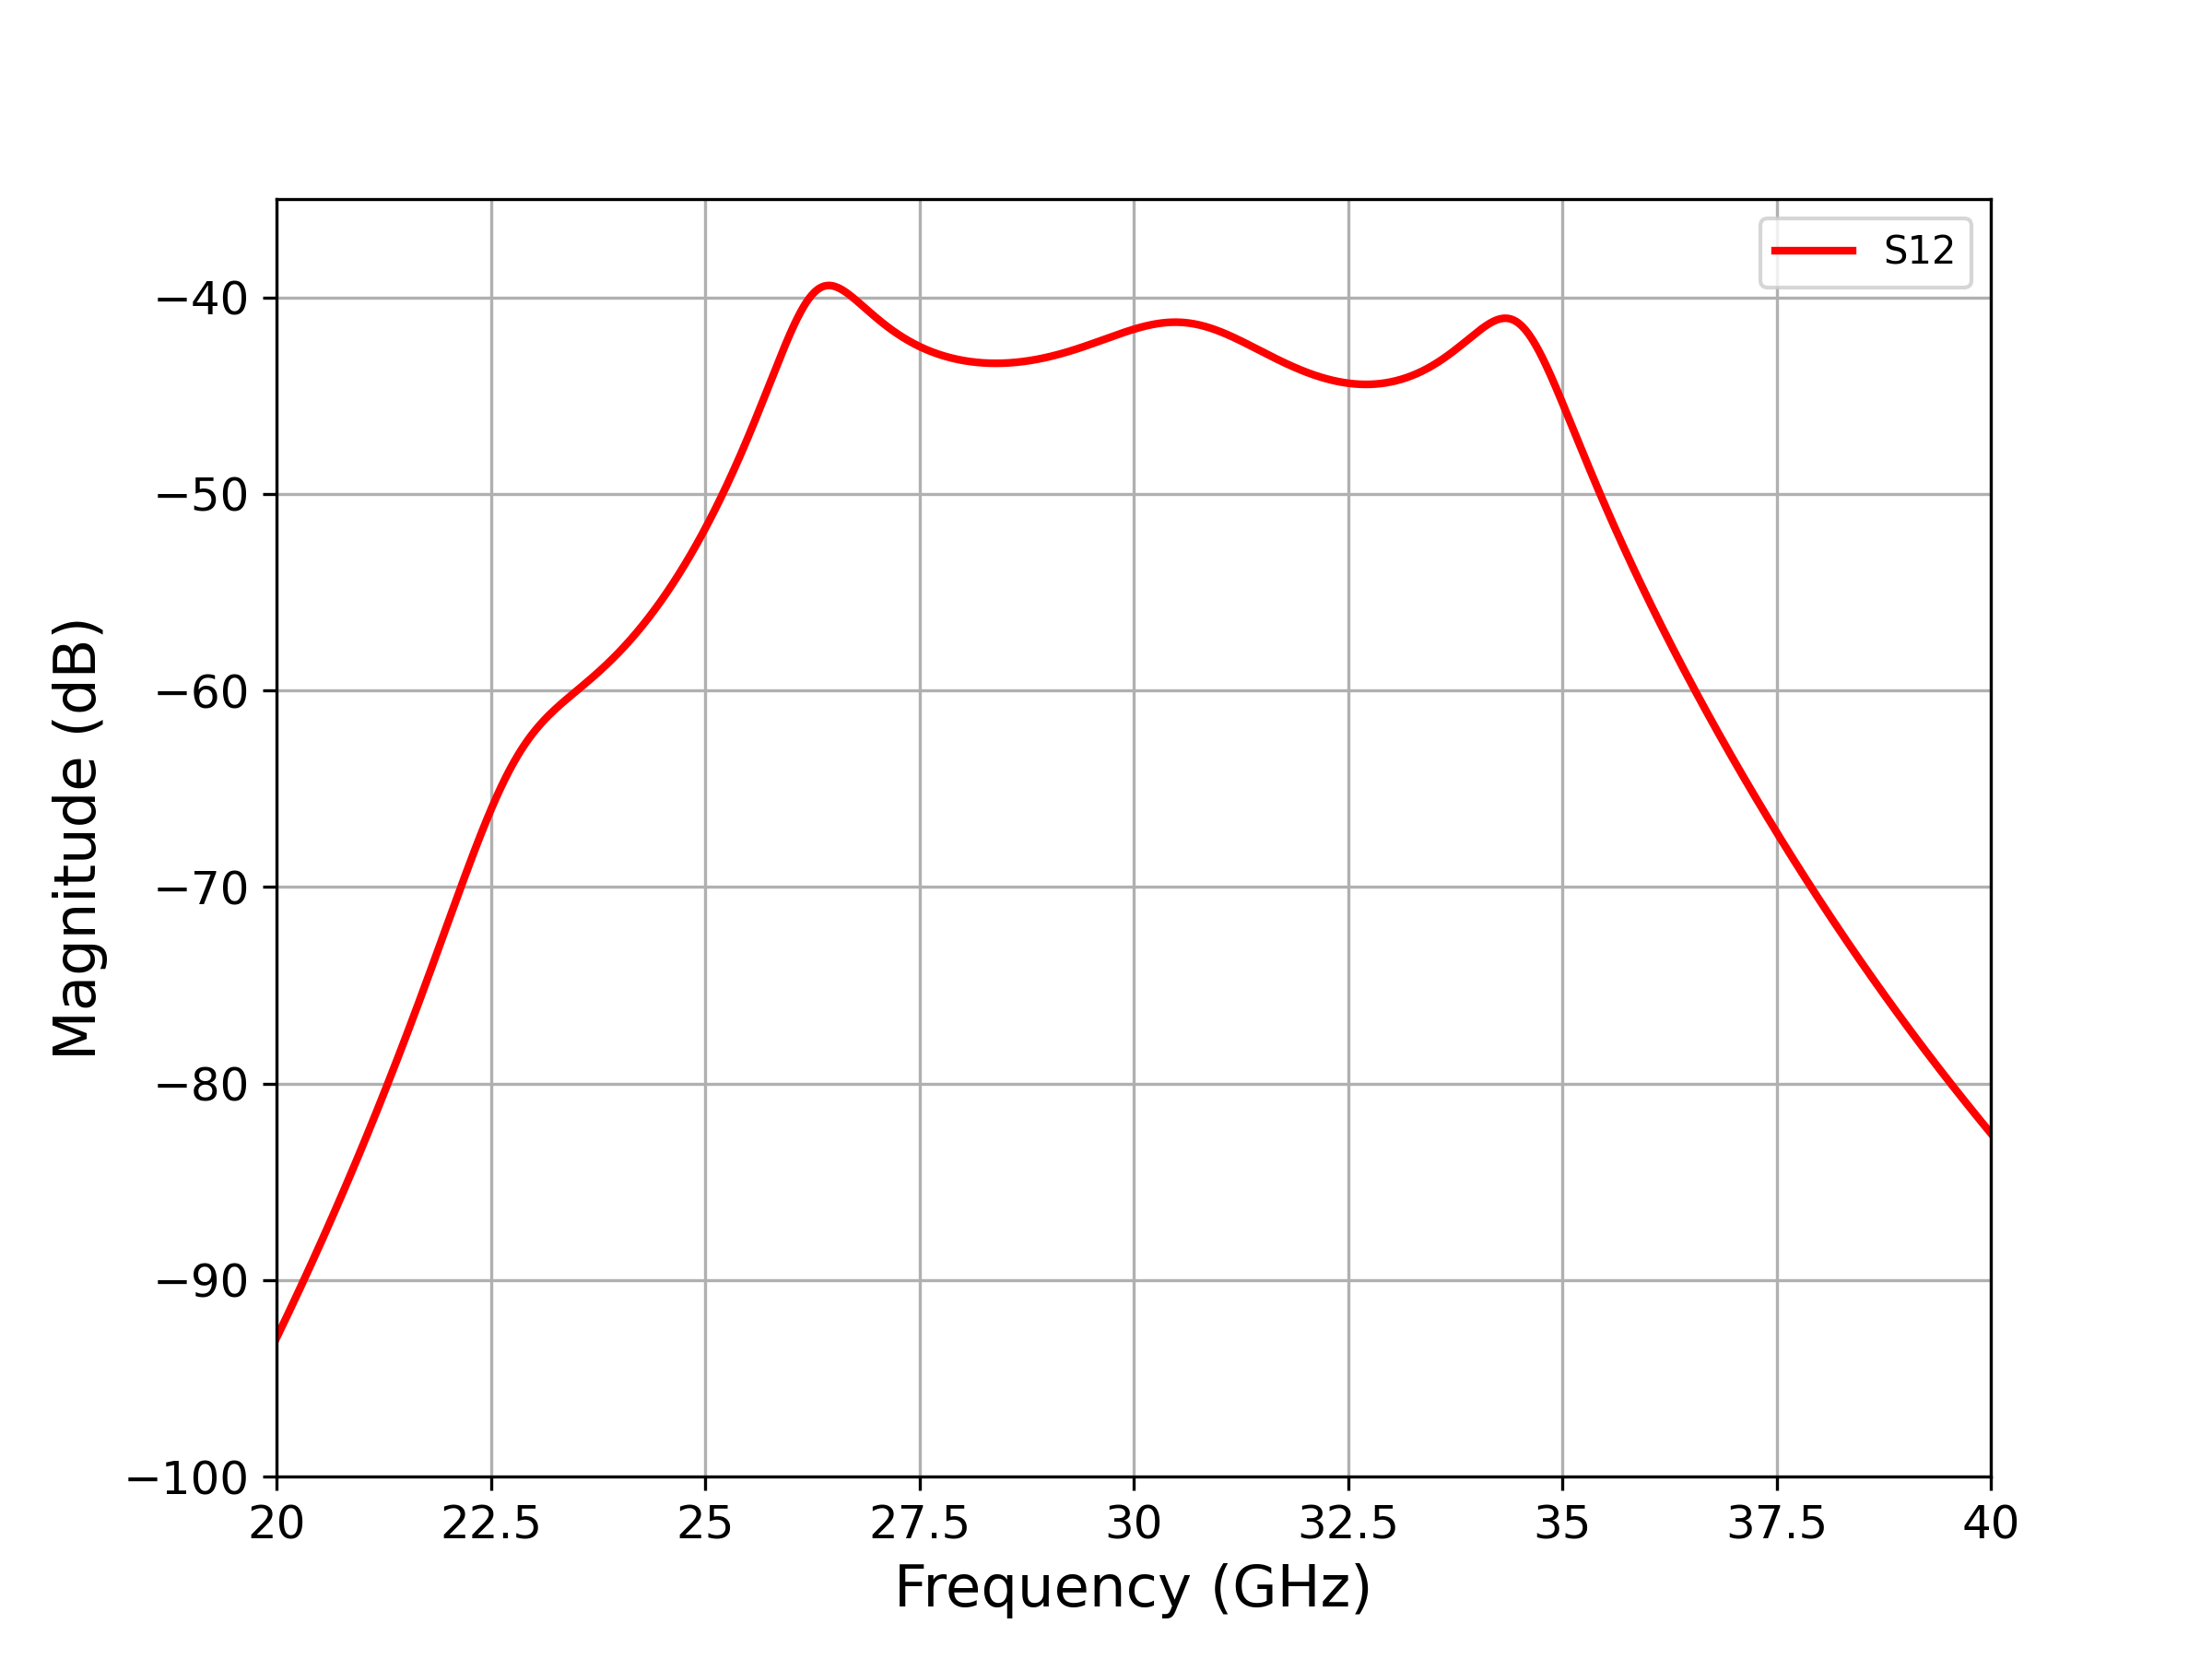
\includegraphics[]{figures/two_stage_withMatching_s12.png}
%     }
%     \caption{$S_{12}$ parameter of a two-stage power amplifier (shown in Figure \ref{fig:two-stage-with-input-interstage-matching}) with input and interstage matching network. The $S_{12}$ parameter is plotted from 0 GHz to 60 GHz.}
%     \label{fig:two-stage-withmatching-cadence-s12}
% \end{figure}

\begin{figure}[H]
  \centering
  \begin{subfigure}{0.49\textwidth}
    \centering
    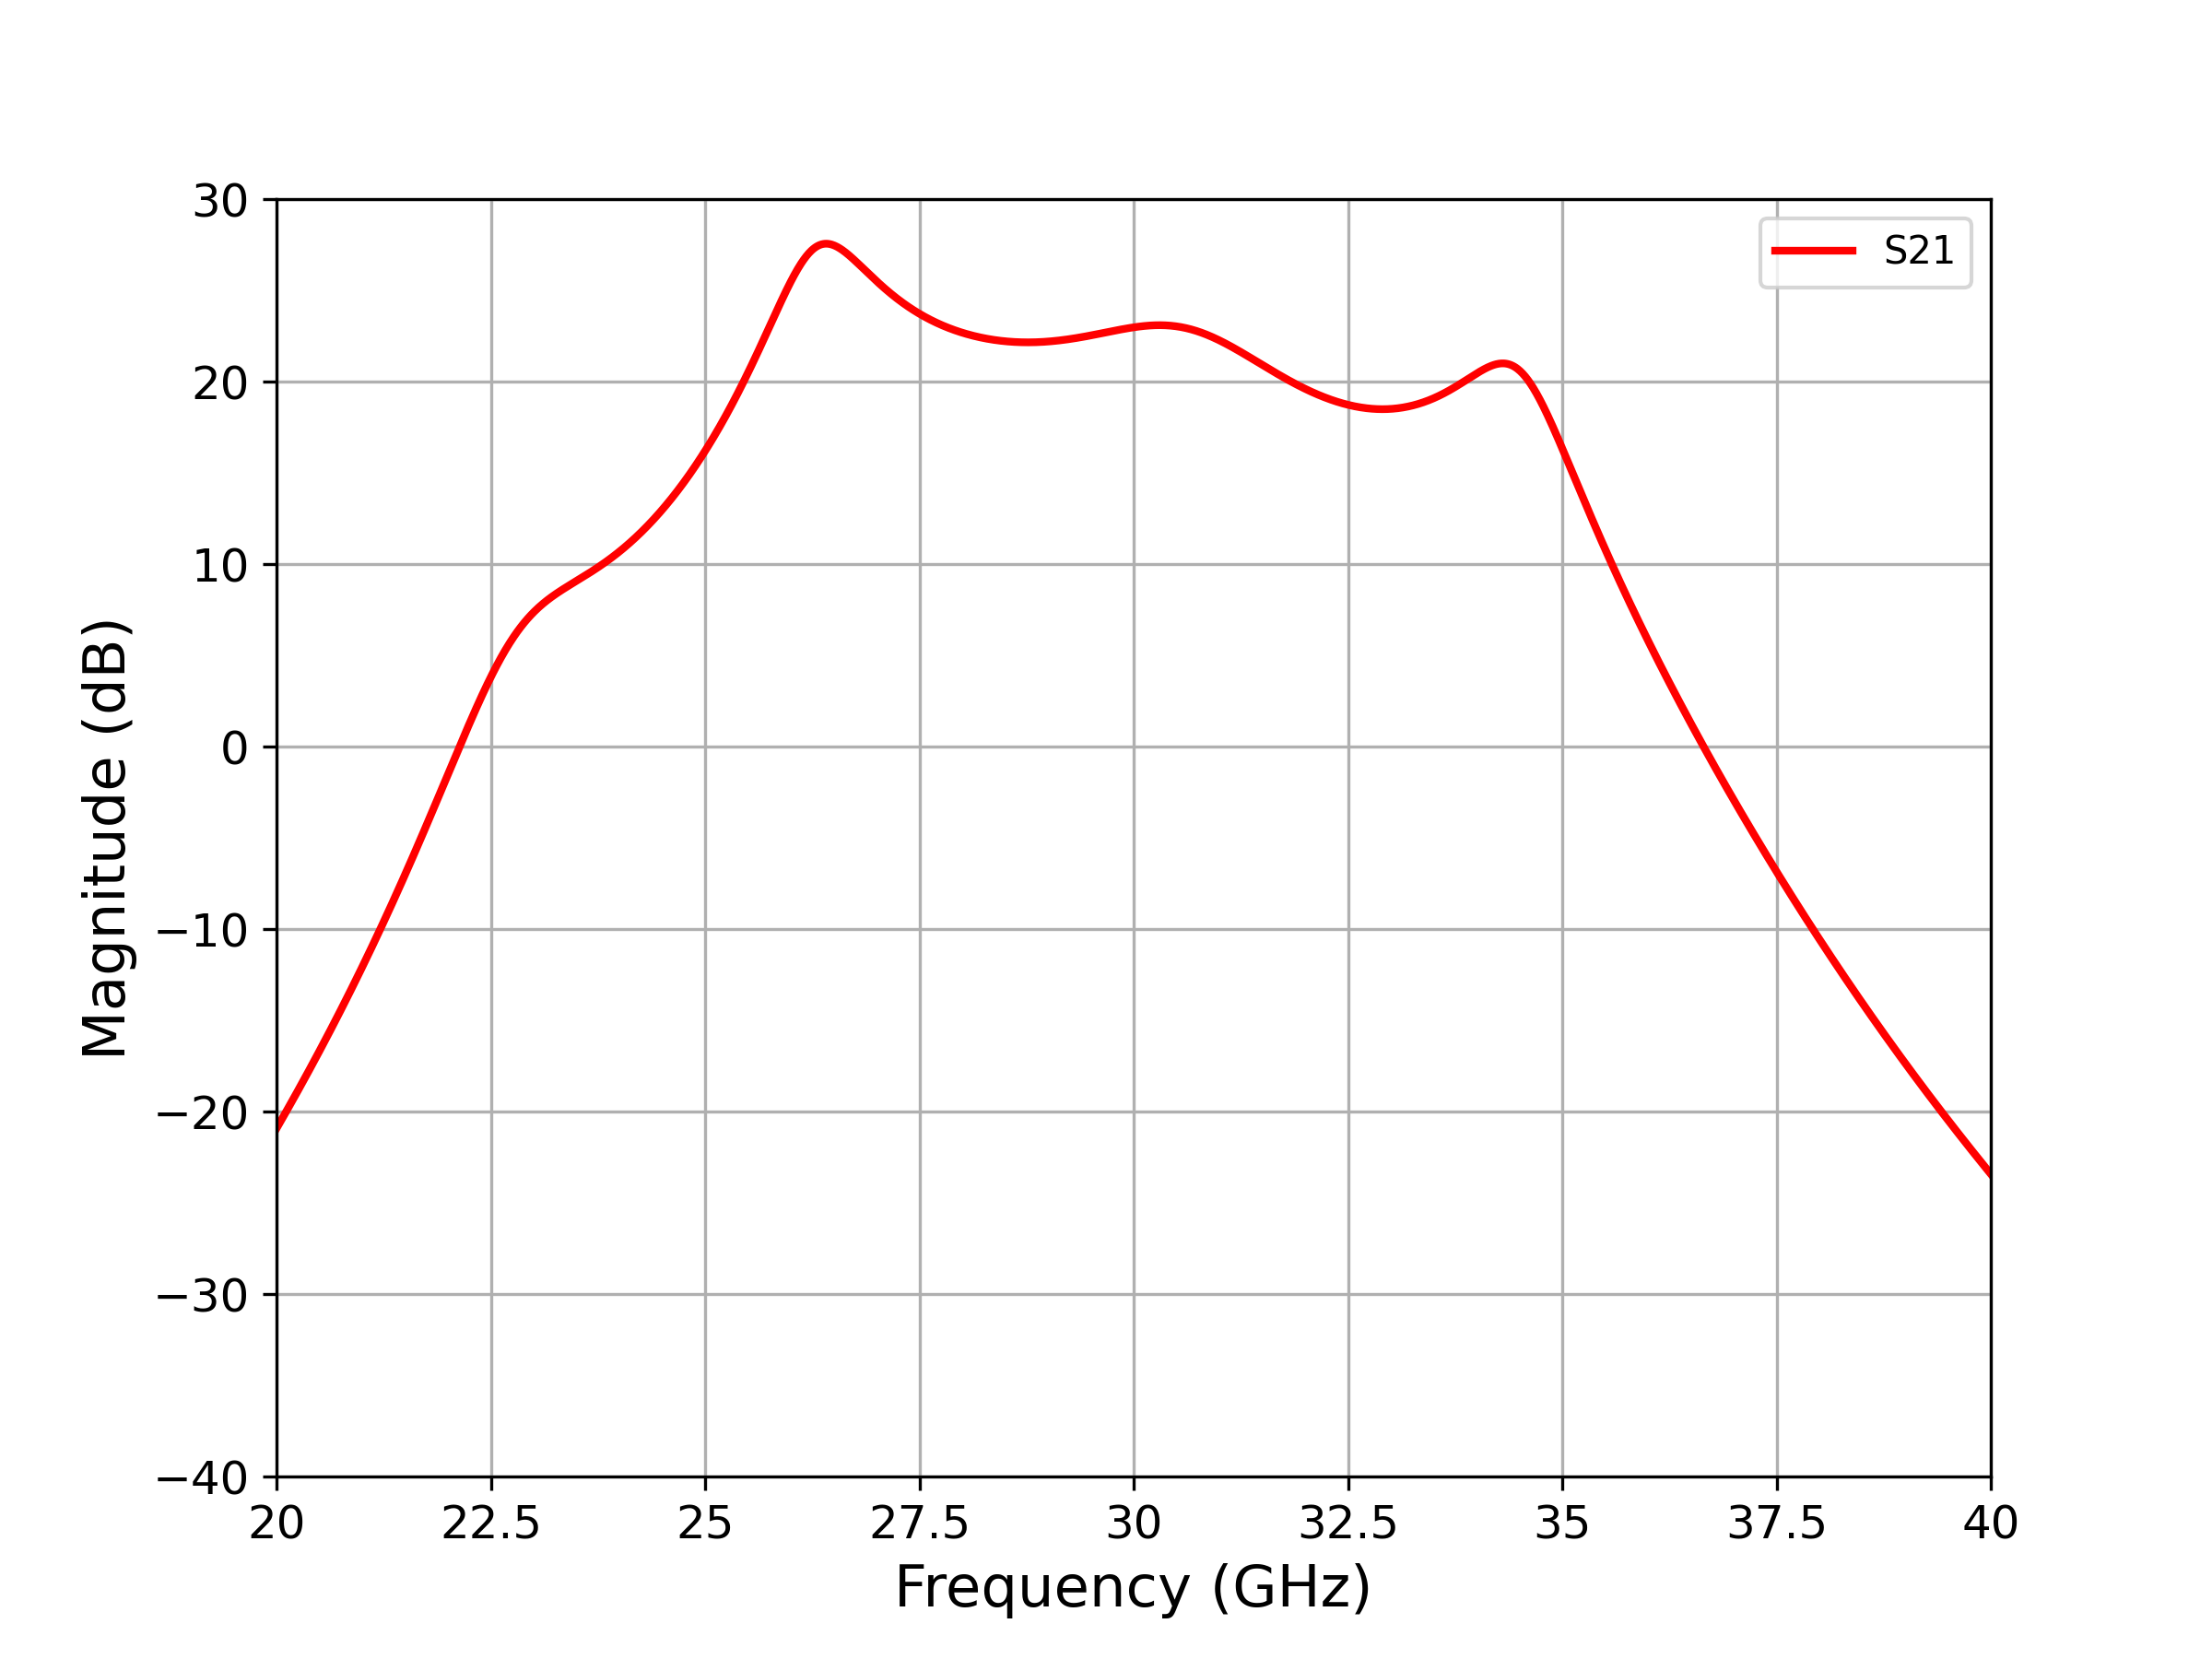
\includegraphics[width=\linewidth]{figures/two_stage_withMatching_s21.png}
    \caption{}
    \label{fig:two-stage-withmatching-cadence-s21}
  \end{subfigure}
  \hfill
  \begin{subfigure}{0.49\textwidth}
    \centering
    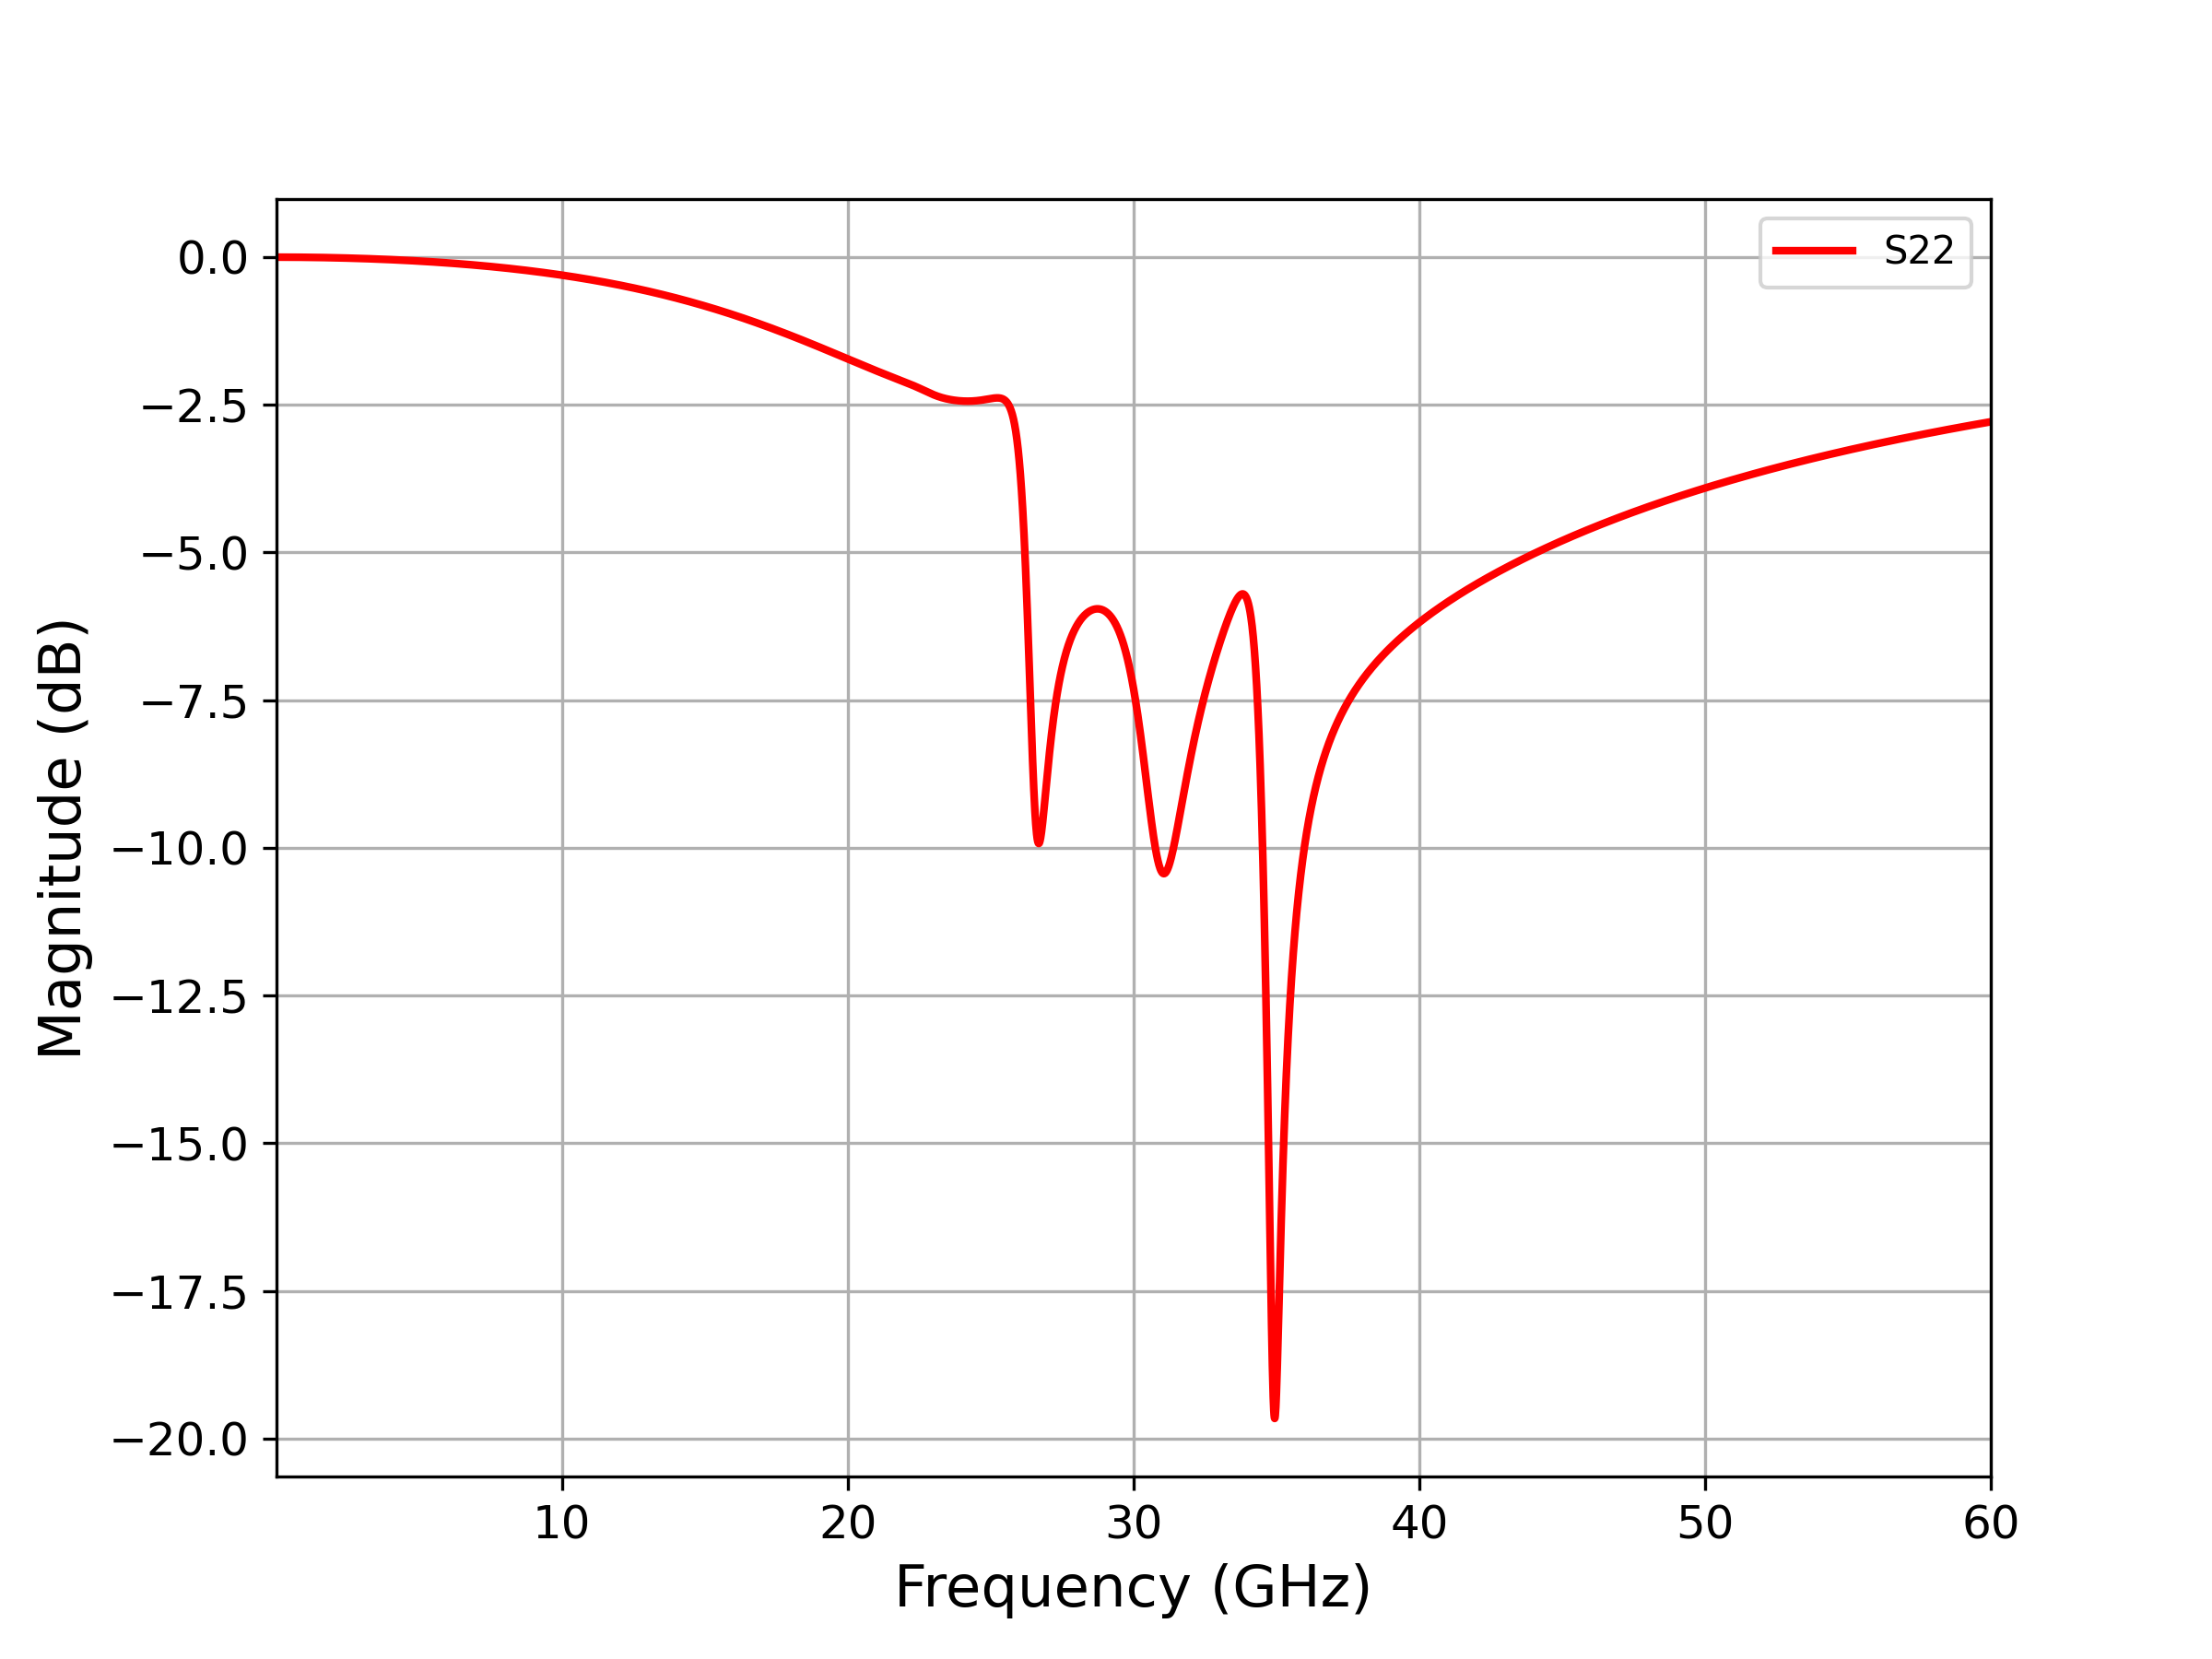
\includegraphics[width=\linewidth]{figures/two_stage_withMatching_s22.png}
    \caption{}
     \label{fig:two-stage-withmatching-cadence-s22}
  \end{subfigure}
  \caption{(a) $S_{21}$ parameter of a two-stage power amplifier (shown in Figure \ref{fig:two-stage-with-input-interstage-matching}) with input and interstage matching network. (b) $S_{22}$ parameter of a two-stage power amplifier (shown in Figure \ref{fig:two-stage-with-input-interstage-matching}) with input and interstage matching network.}
  \label{fig:two-stage-withmatching-cadence-s21-s22}
\end{figure}

The maximum value of $S_{21}$ at 26.41 GHz is 27.55 dB, indicating a
higher power gain compared to the previous stages. Average gain and
gain at matching frequencies: The average gain across the frequency range
of 25 to 35 GHz is 21.78 dB. At the matching frequencies of 27.12 GHz and
32.33 GHz, the gain values are 25 dB and 18.96 dB, respectively. These
gains demonstrate the improvement achieved through the matching network. The proposed PA exhibits good output matching
with $S_{22}$ values of less than -5 dB, indicating that a small portion of the
output power is reflected back.
% \begin{figure}[H]
%     \centering
%     \resizebox{0.8\textwidth}{!}{
%     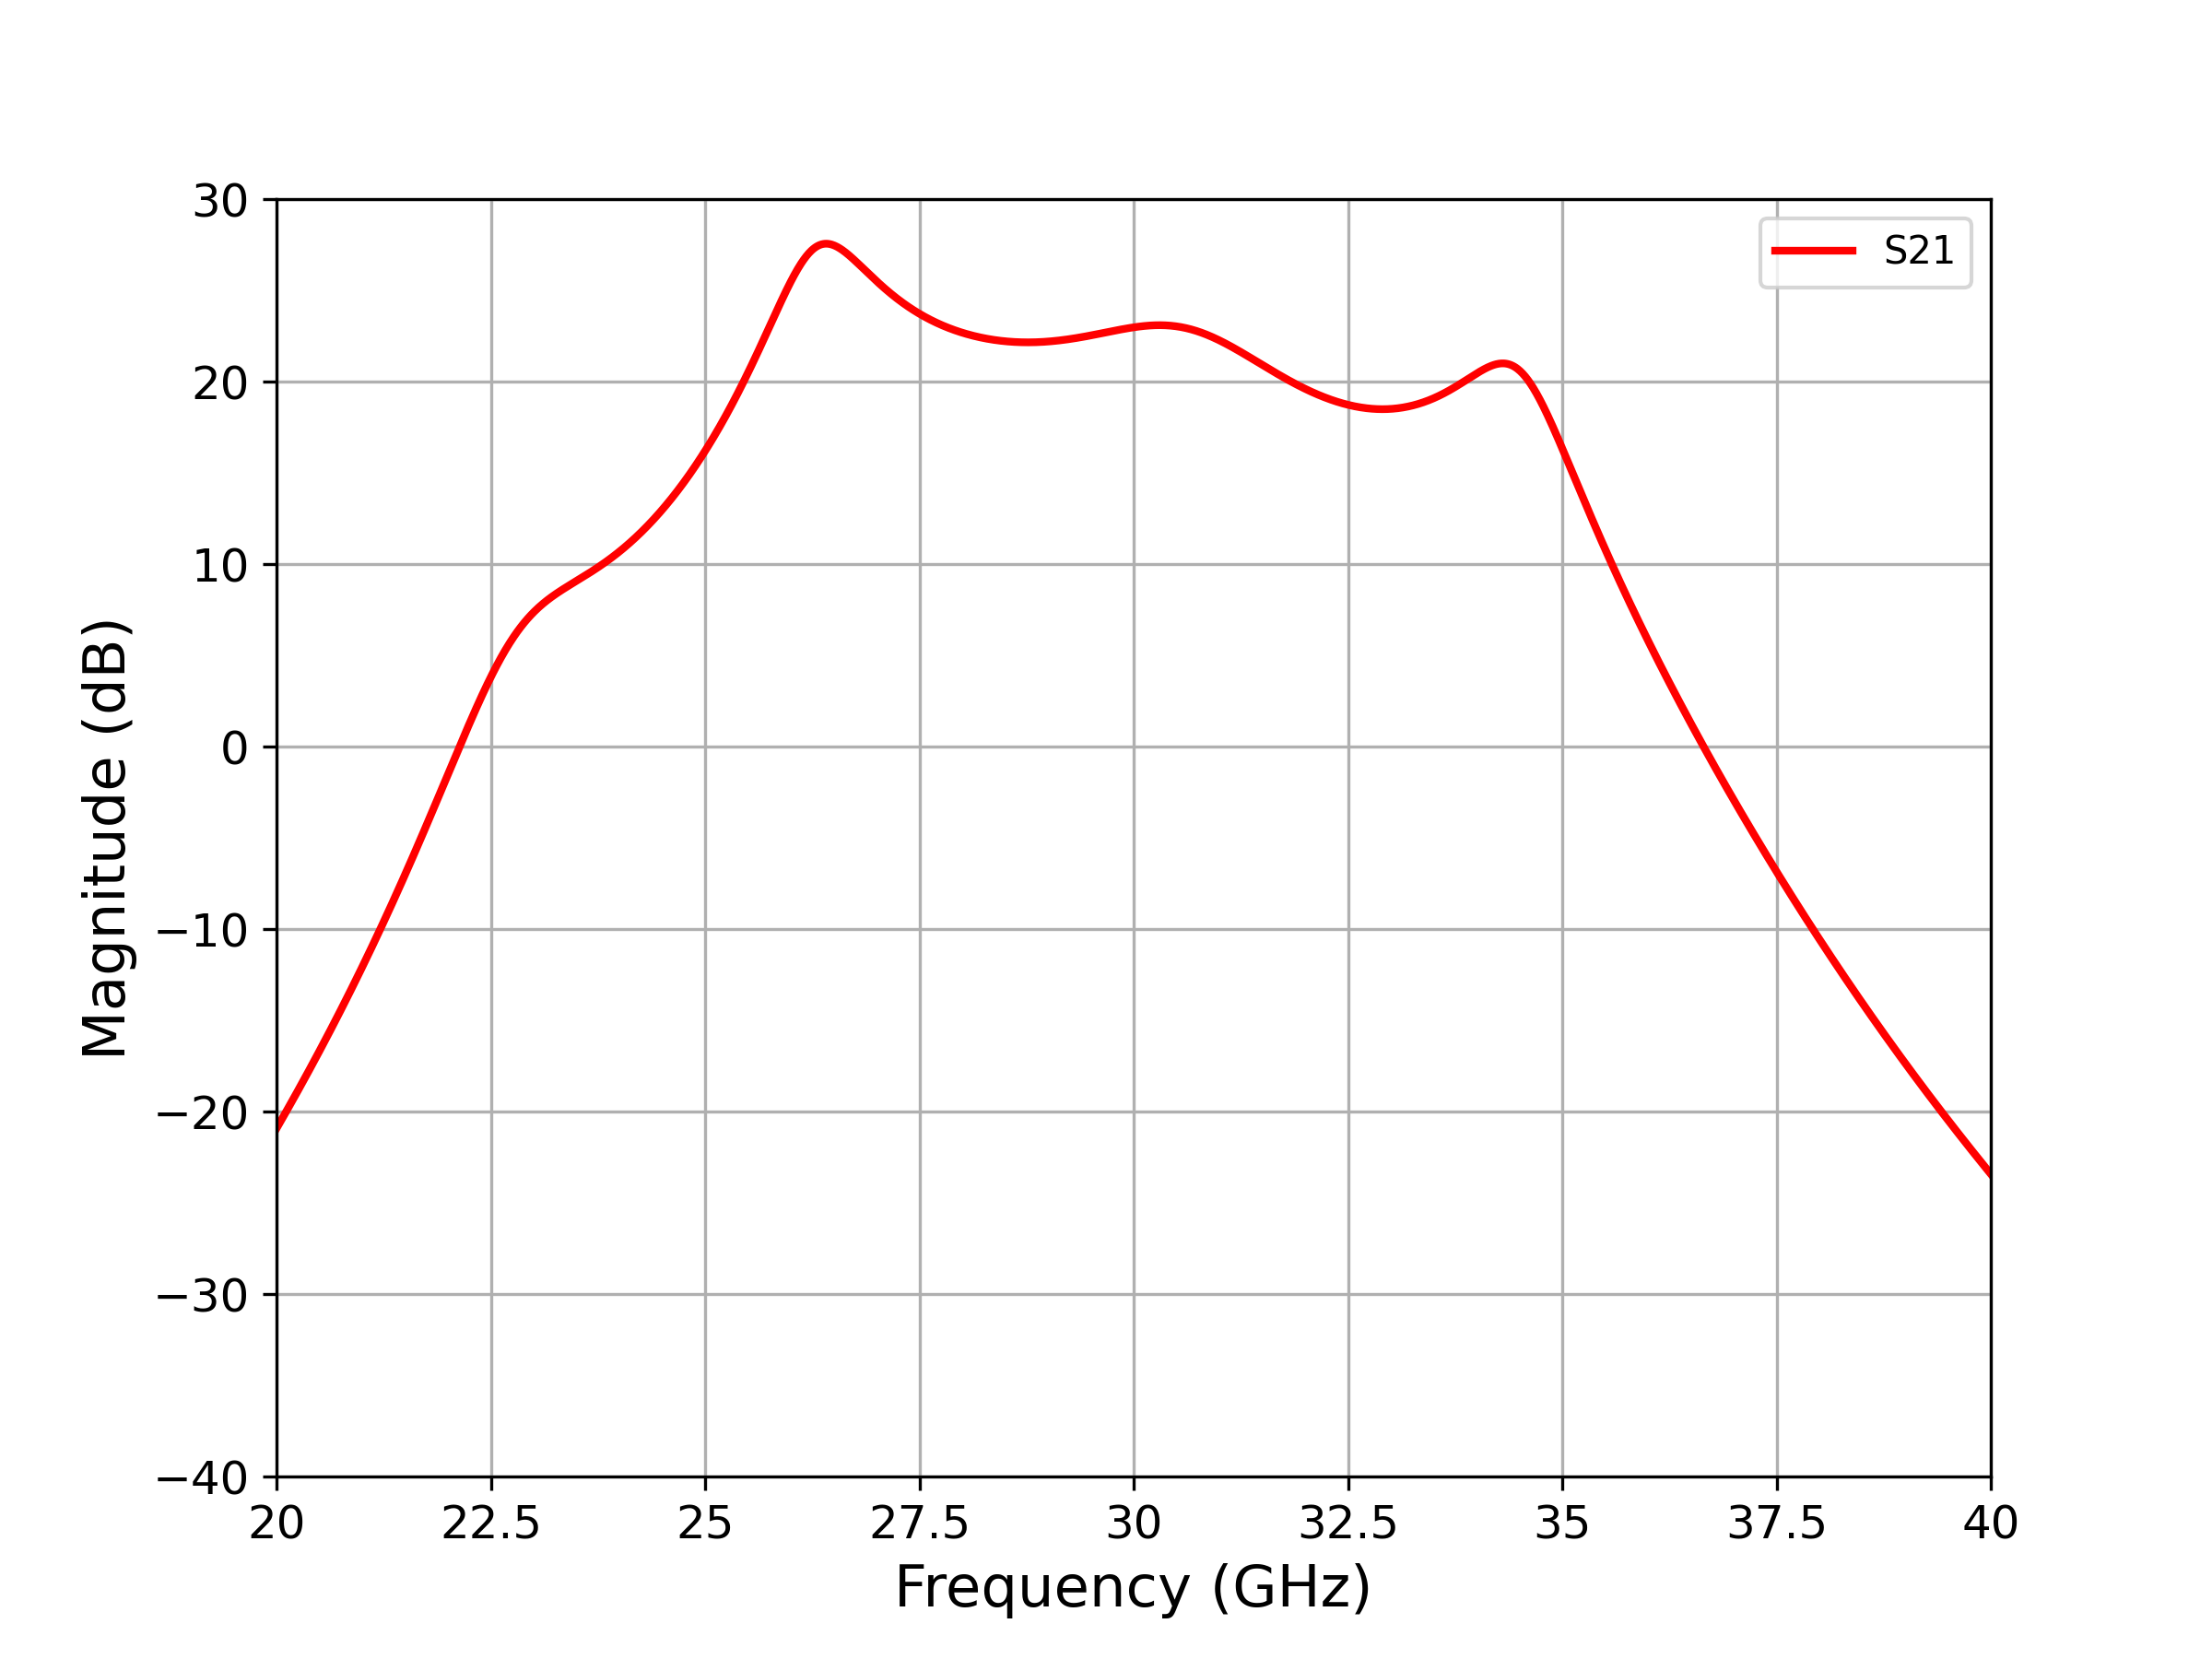
\includegraphics[]{figures/two_stage_withMatching_s21.png}
%     }
%     \caption{$S_{21}$ parameter of a two-stage power amplifier (shown in Figure \ref{fig:two-stage-with-input-interstage-matching}) with input and interstage matching network. The $S_{21}$ parameter is plotted from 20 GHz to 40 GHz.}
%     \label{fig:two-stage-withmatching-cadence-s21}
% \end{figure}
% \begin{figure}[H]
%     \centering
%     \resizebox{0.8\textwidth}{!}{
%     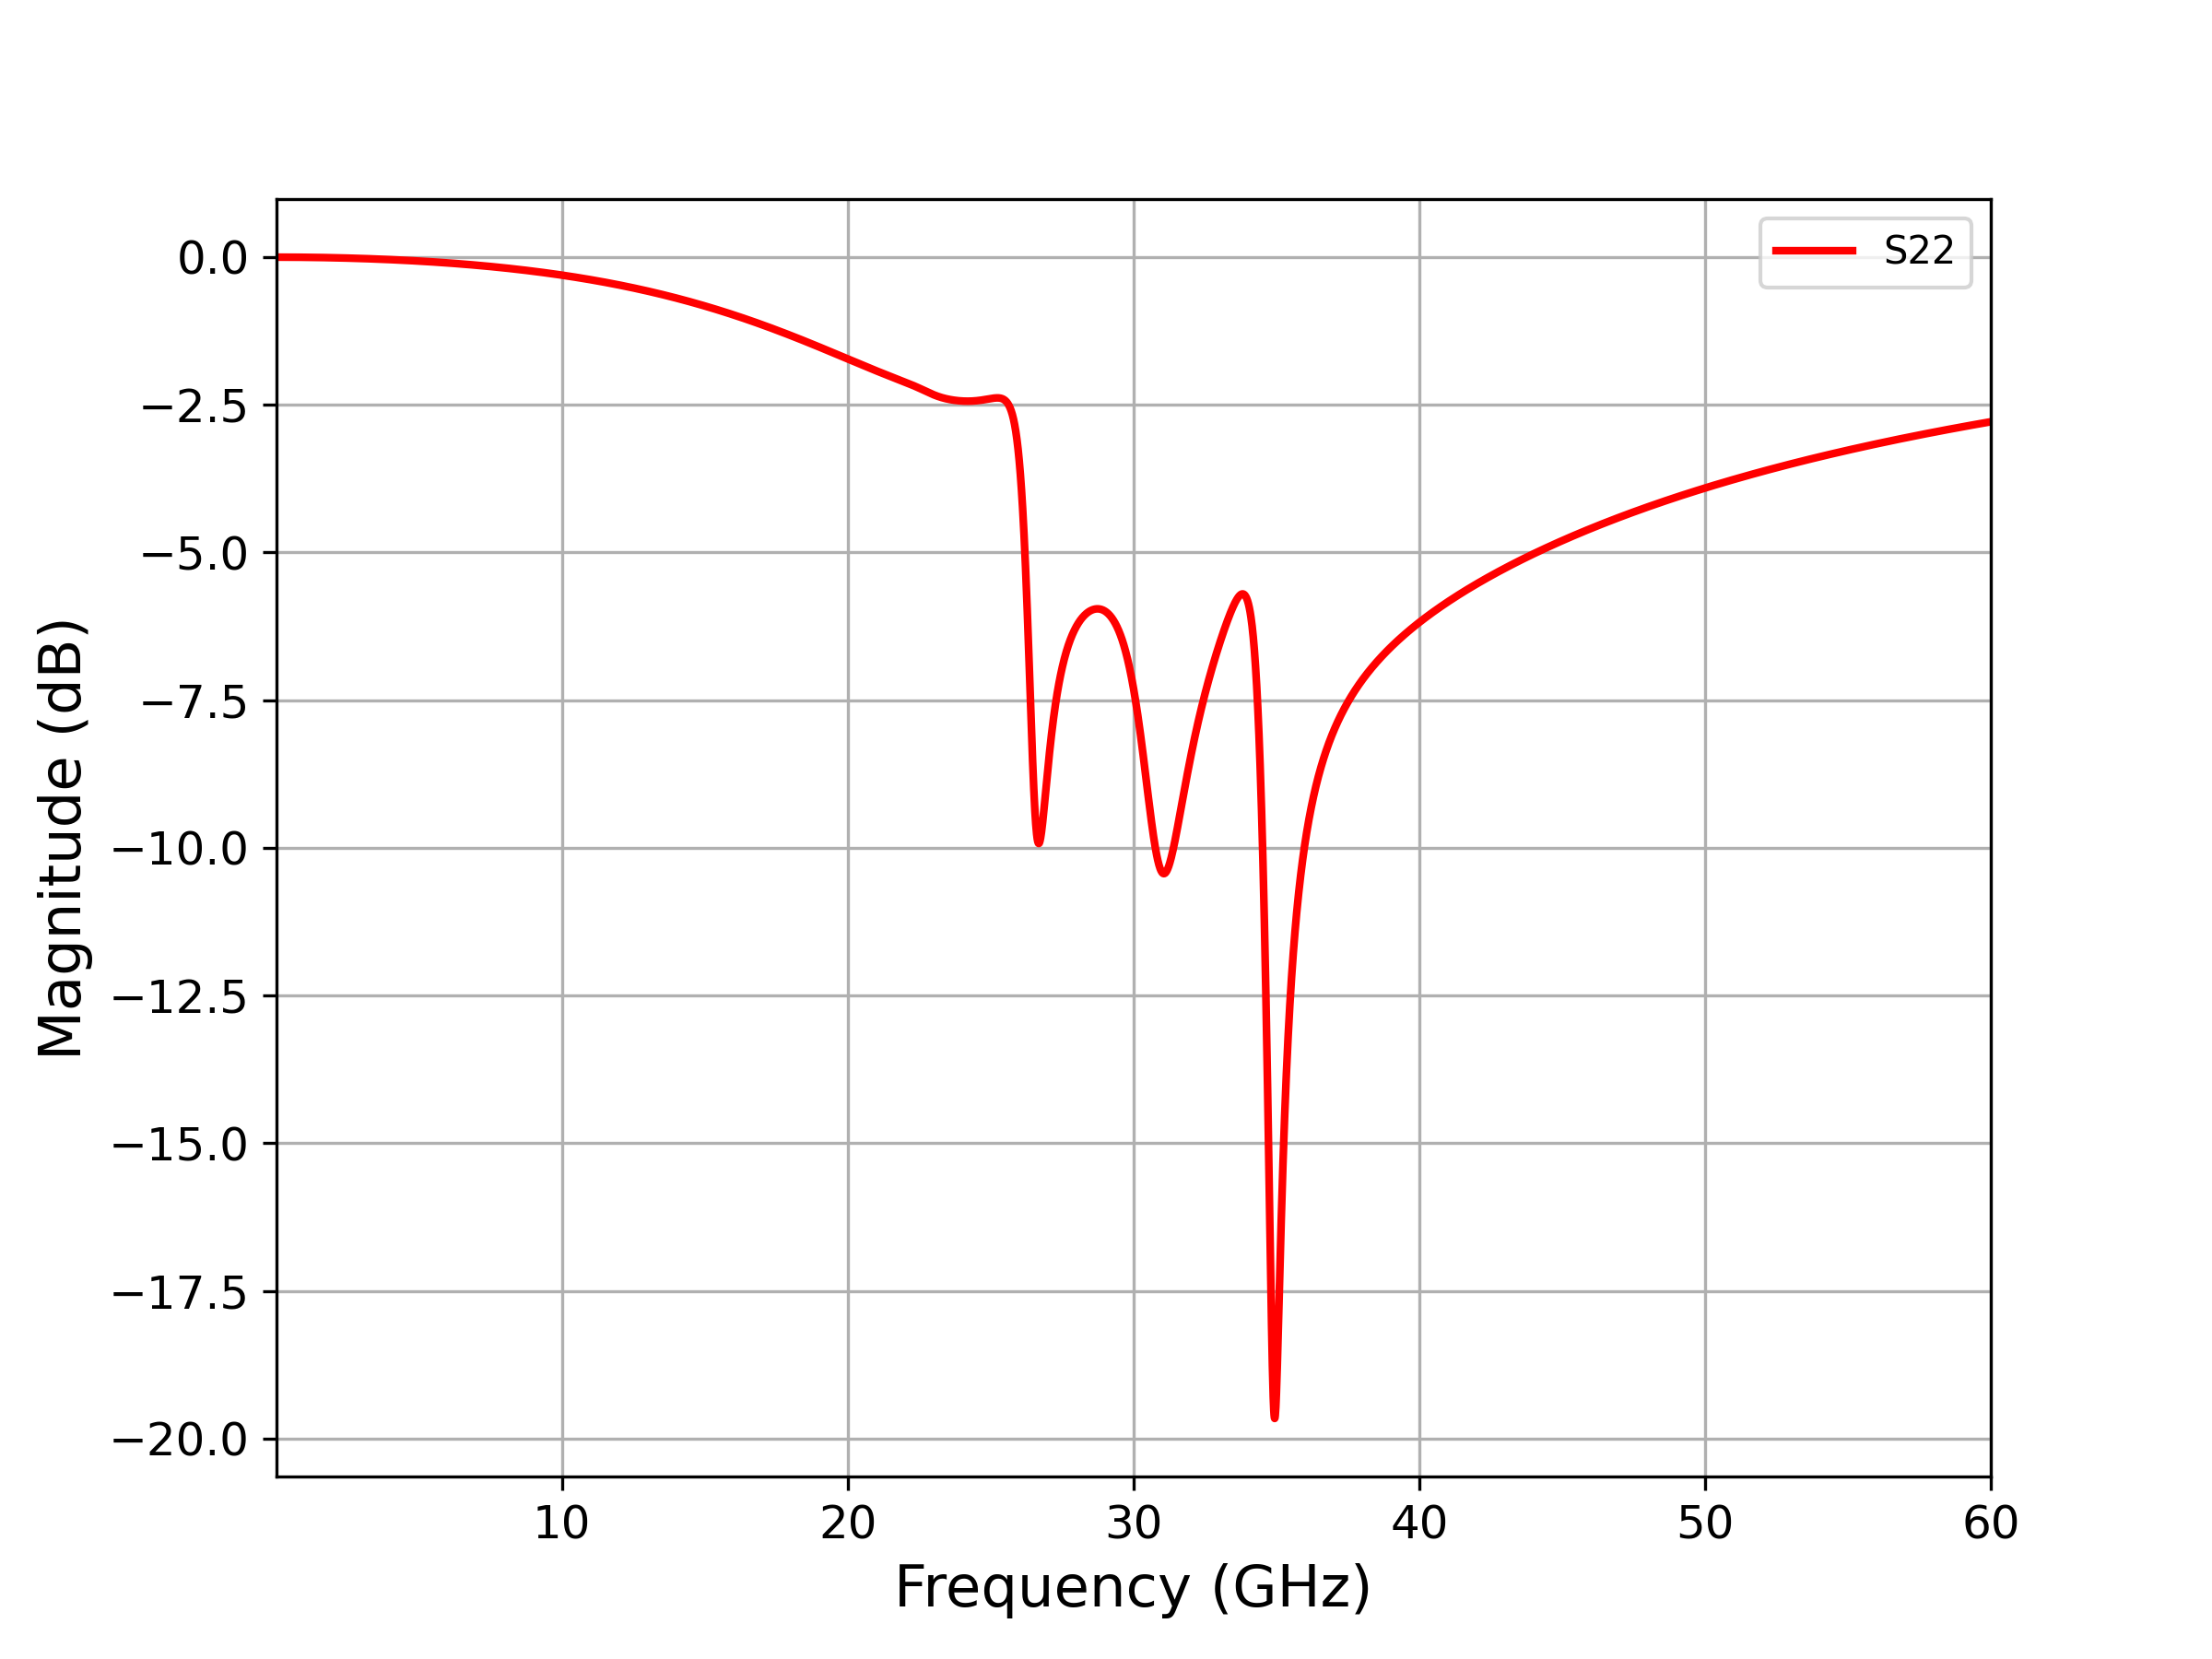
\includegraphics[]{figures/two_stage_withMatching_s22.png}
%     }
%     \caption{$S_{22}$ parameter of a two-stage power amplifier (shown in Figure \ref{fig:two-stage-with-input-interstage-matching}) with input and interstage matching network. The $S_{22}$ parameter is plotted from 0 GHz to 60 GHz.}
%     \label{fig:two-stage-withmatching-cadence-s22}
% \end{figure}
\begin{figure}[H]
  \centering
  \begin{subfigure}{0.49\textwidth}
    \centering
    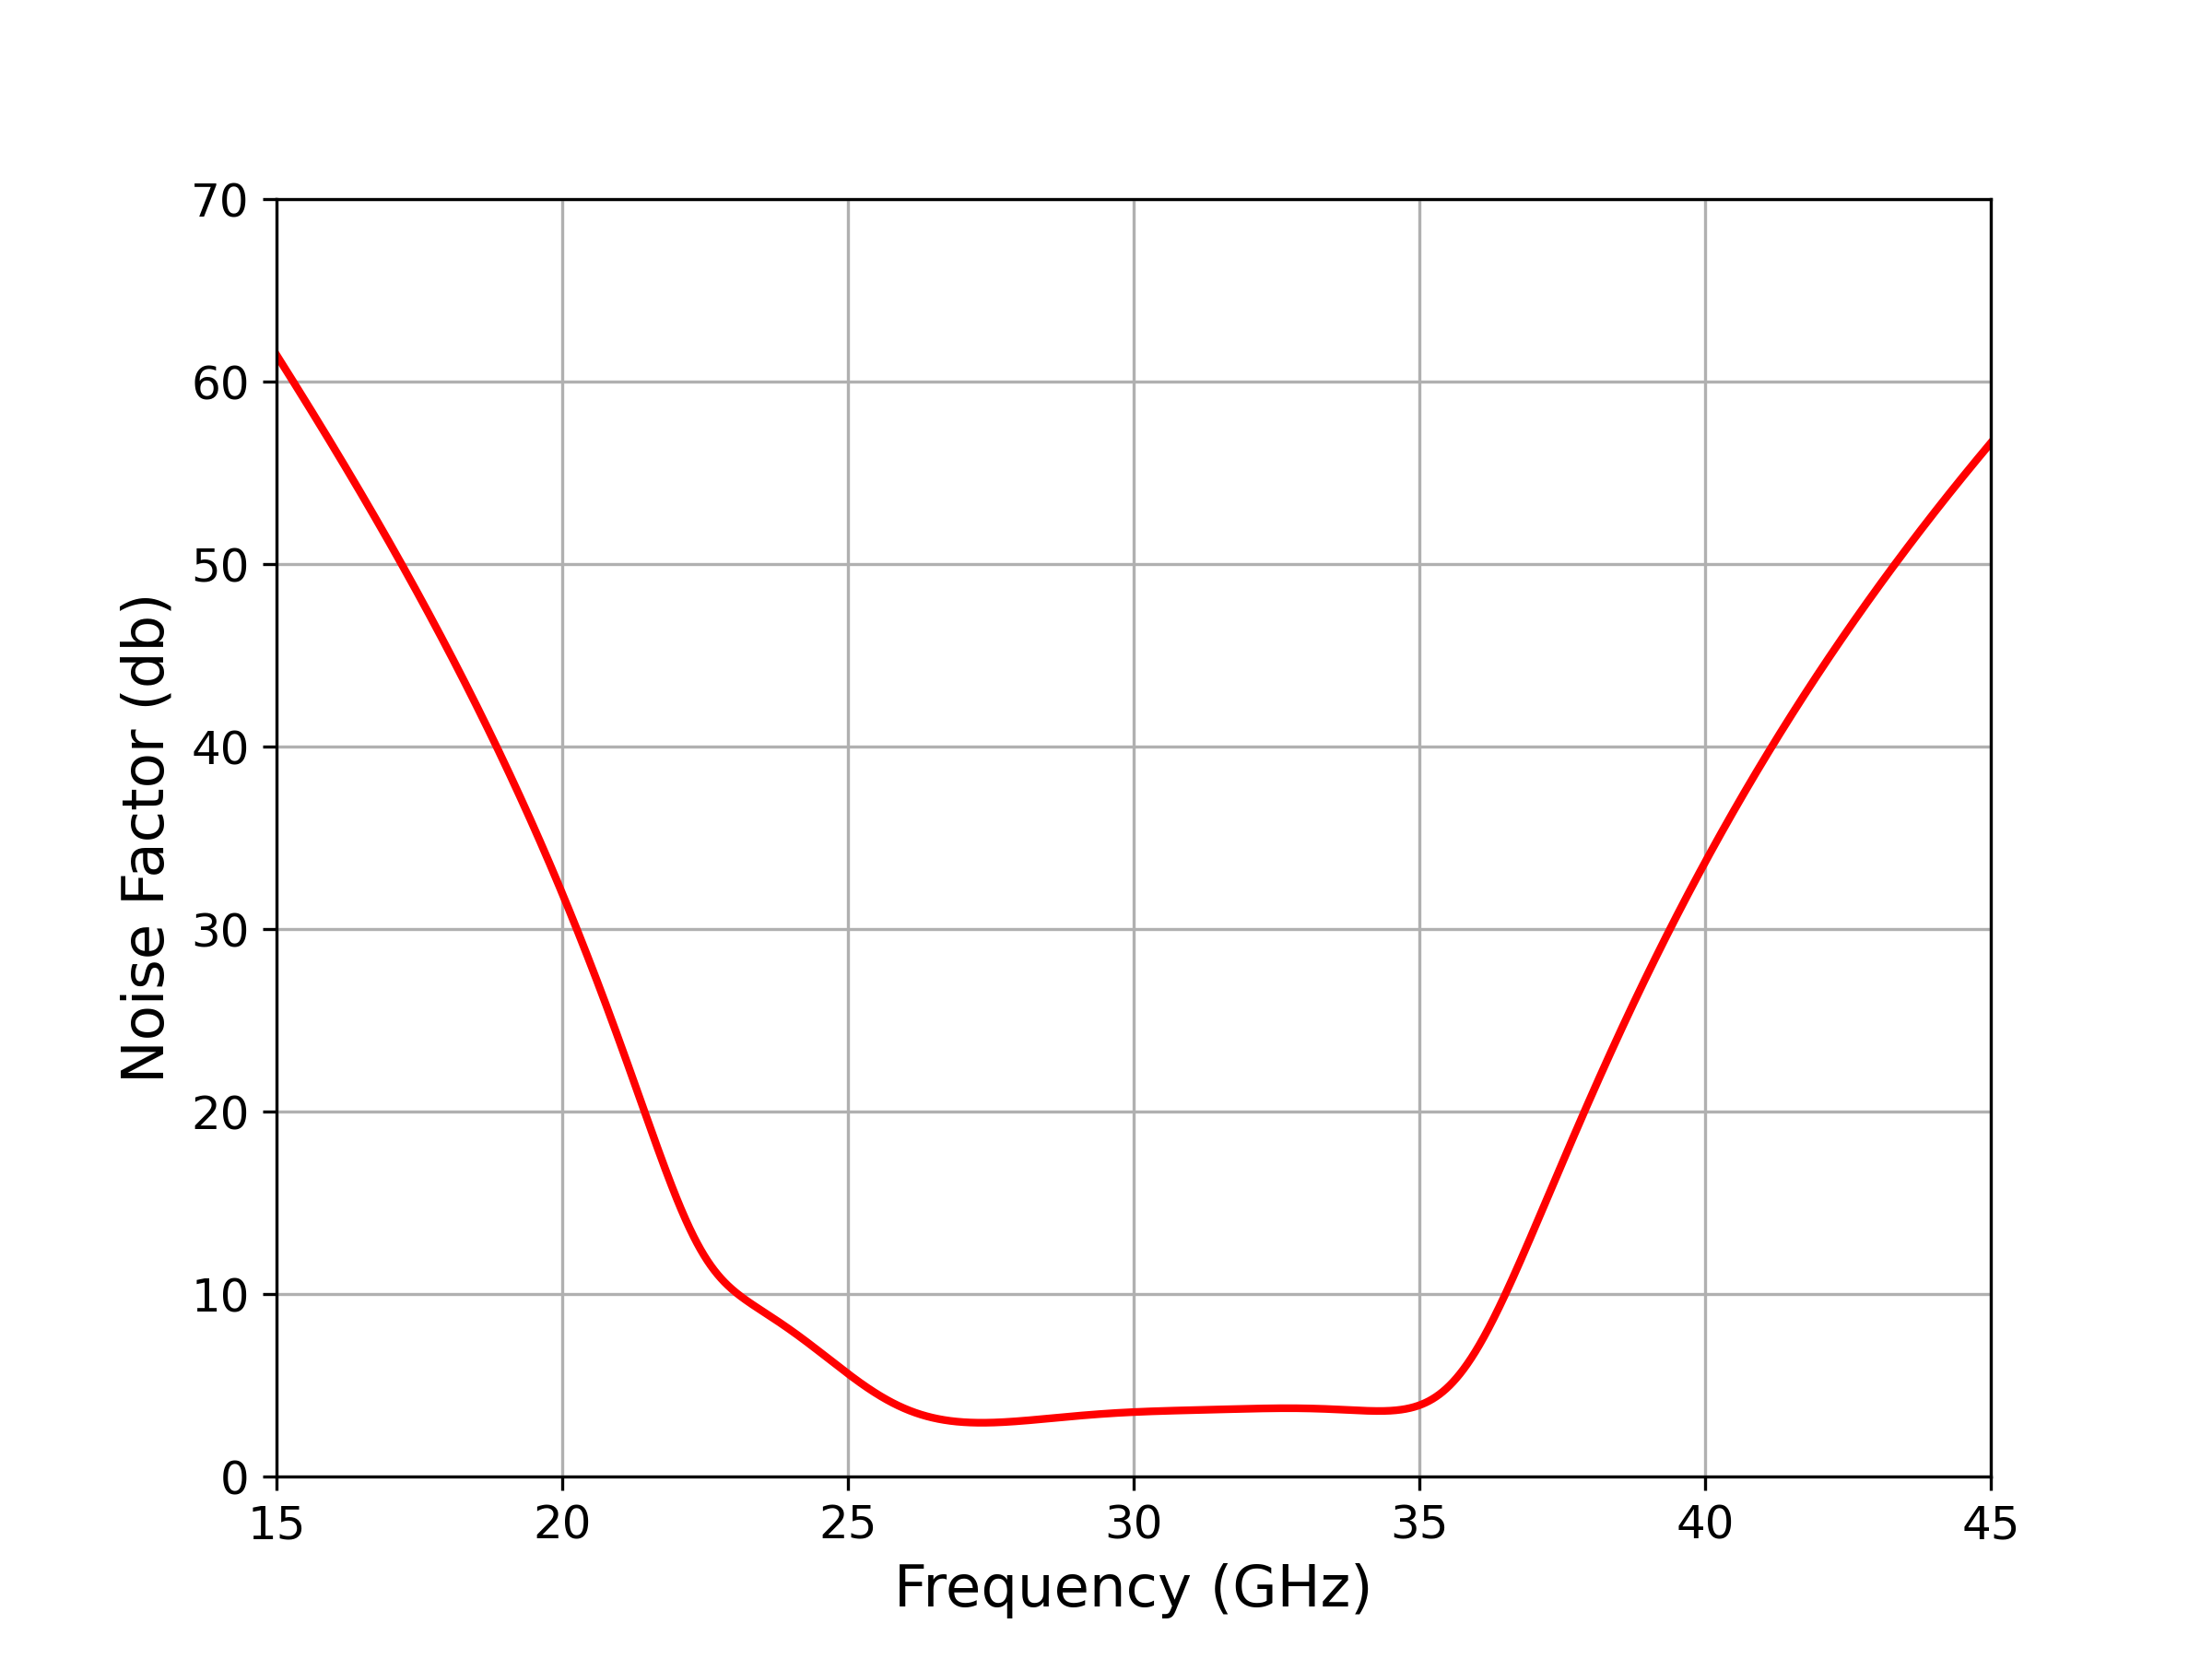
\includegraphics[width=\linewidth]{figures/noise-factor.png}
    \caption{}
    \label{fig:noise-factor}
  \end{subfigure}
  \hfill
  \begin{subfigure}{0.49\textwidth}
    \centering
    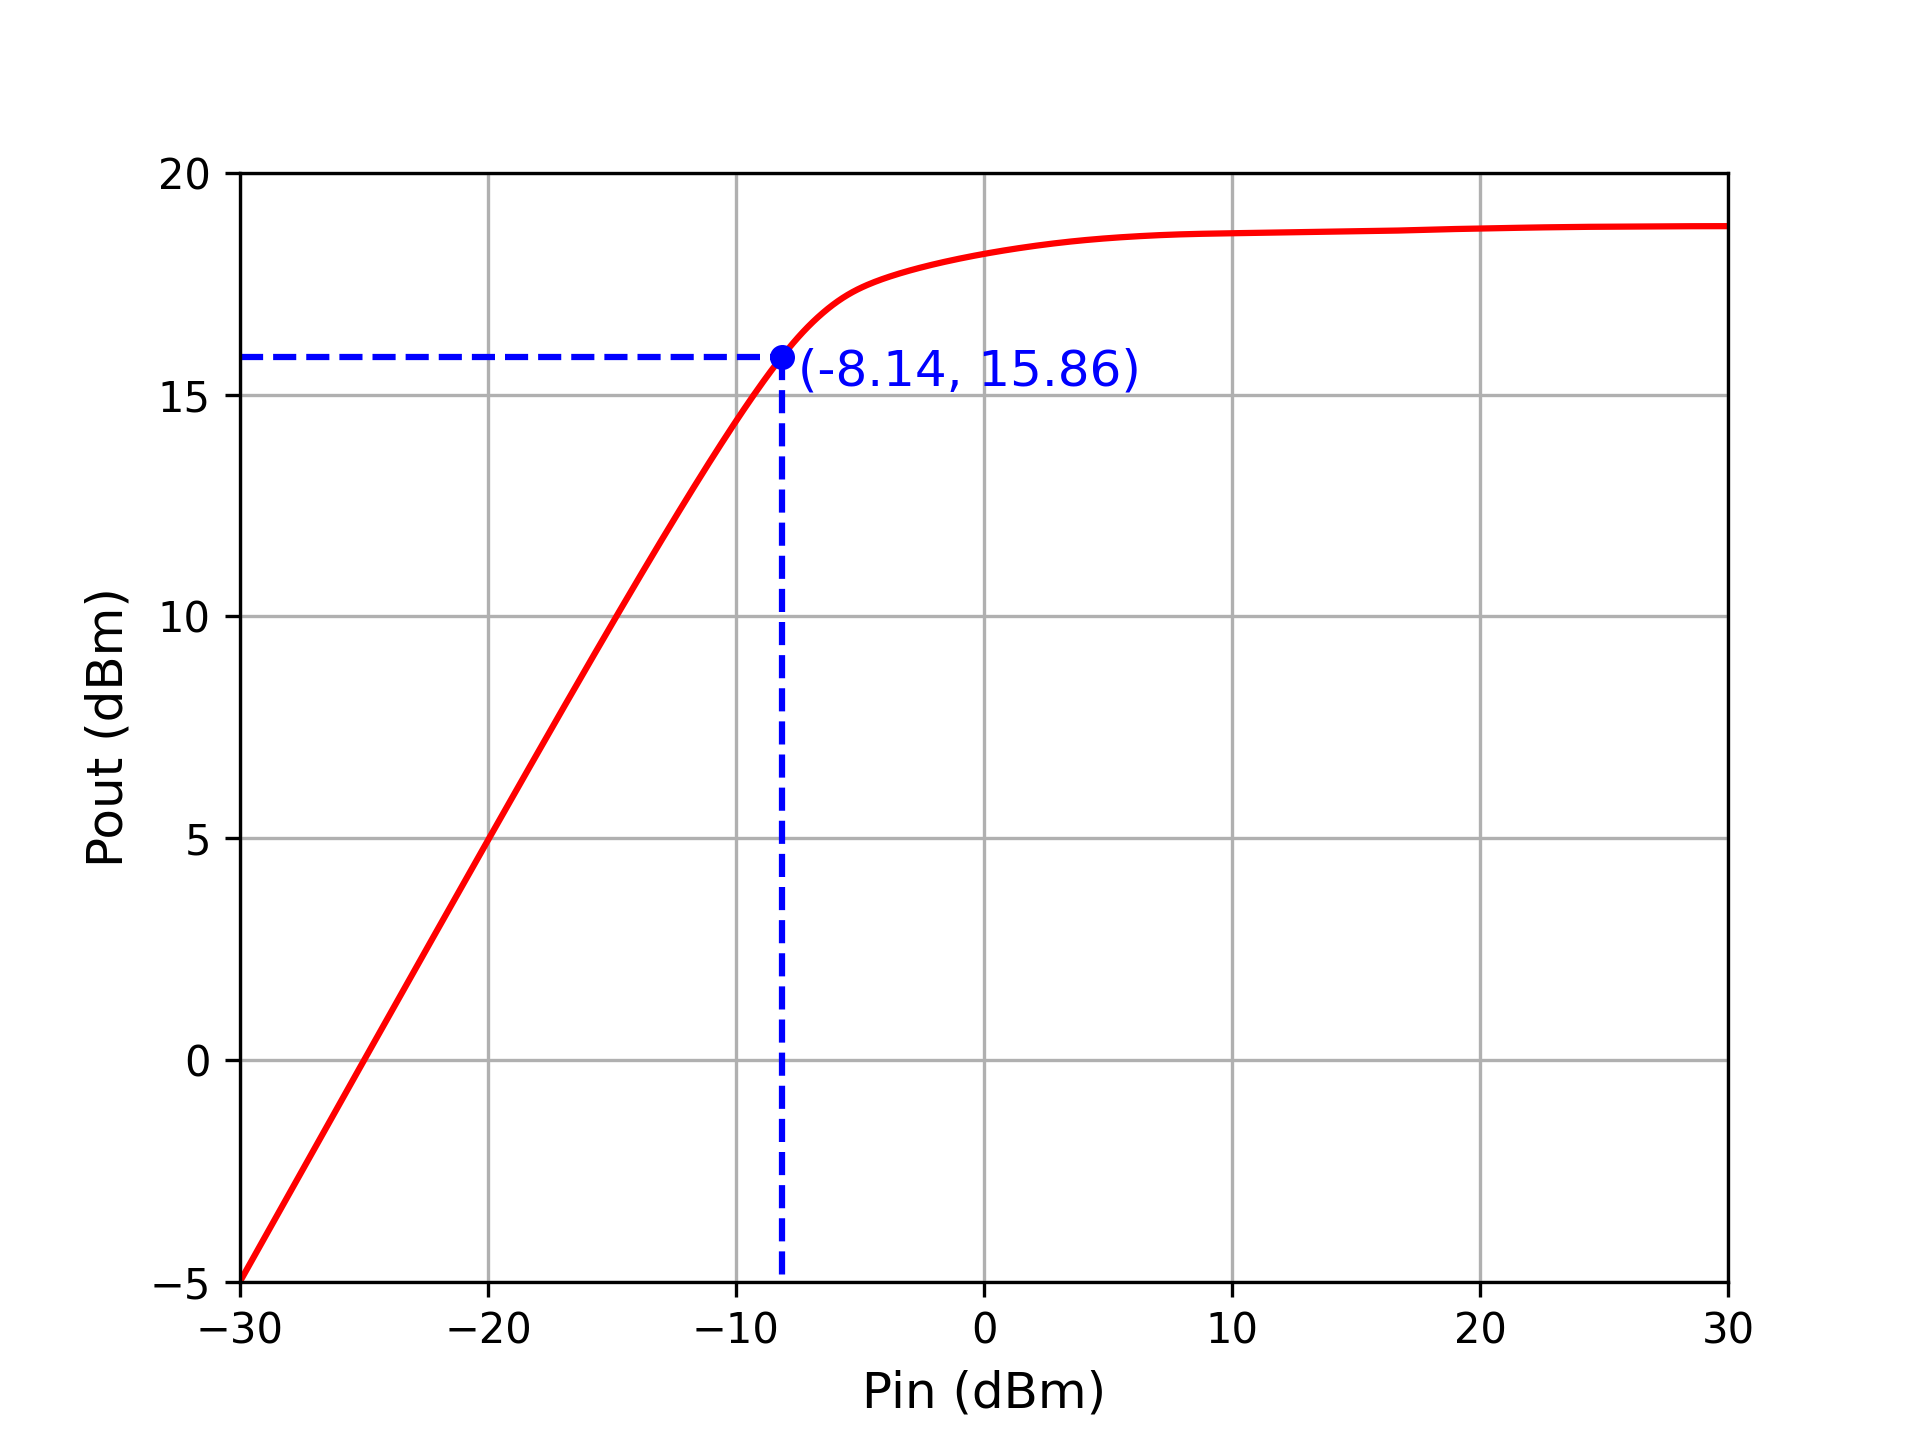
\includegraphics[width=\linewidth]{figures/compressionCurves.png}
    \caption{}
     \label{fig:compression}
  \end{subfigure}
  \caption{(a) Noise factor of a two-stage power amplifier (shown in Figure \ref{fig:two-stage-with-input-interstage-matching}) with input and interstage matching network. (b) P1db compression curve of a two-stage power amplifier (shown in Figure \ref{fig:two-stage-with-input-interstage-matching}) with input and interstage matching network.}
  \label{fig:two-stage-withmatching-cadence-s11-s12}
\end{figure}

The noise factor of a power amplifier is a measure of how much the amplifier degrades the signal-to-noise ratio of the input signal. A lower noise factor indicates better performance, as it means that the amplifier is introducing less additional noise to the signal. Ideally, a power amplifier should have a noise factor as close to 1 as possible, indicating that it adds minimal noise to the input signal. The noise factor of proposed PA is less than 5 dB through 25 GHz to 35 GHz. The P1dB of the proposed PA is (-8.14 dBm,
15.86 dBm). This refers to the output power level at which the gain decreases by
1 dB from its constant value. The $P_{sat}$ value is (12dBm, 18.79dBm) which represents the maximum power level that the amplifier can handle without distortion.
% \begin{figure}[H]
%     \centering
%     \resizebox{0.8\textwidth}{!}{
%     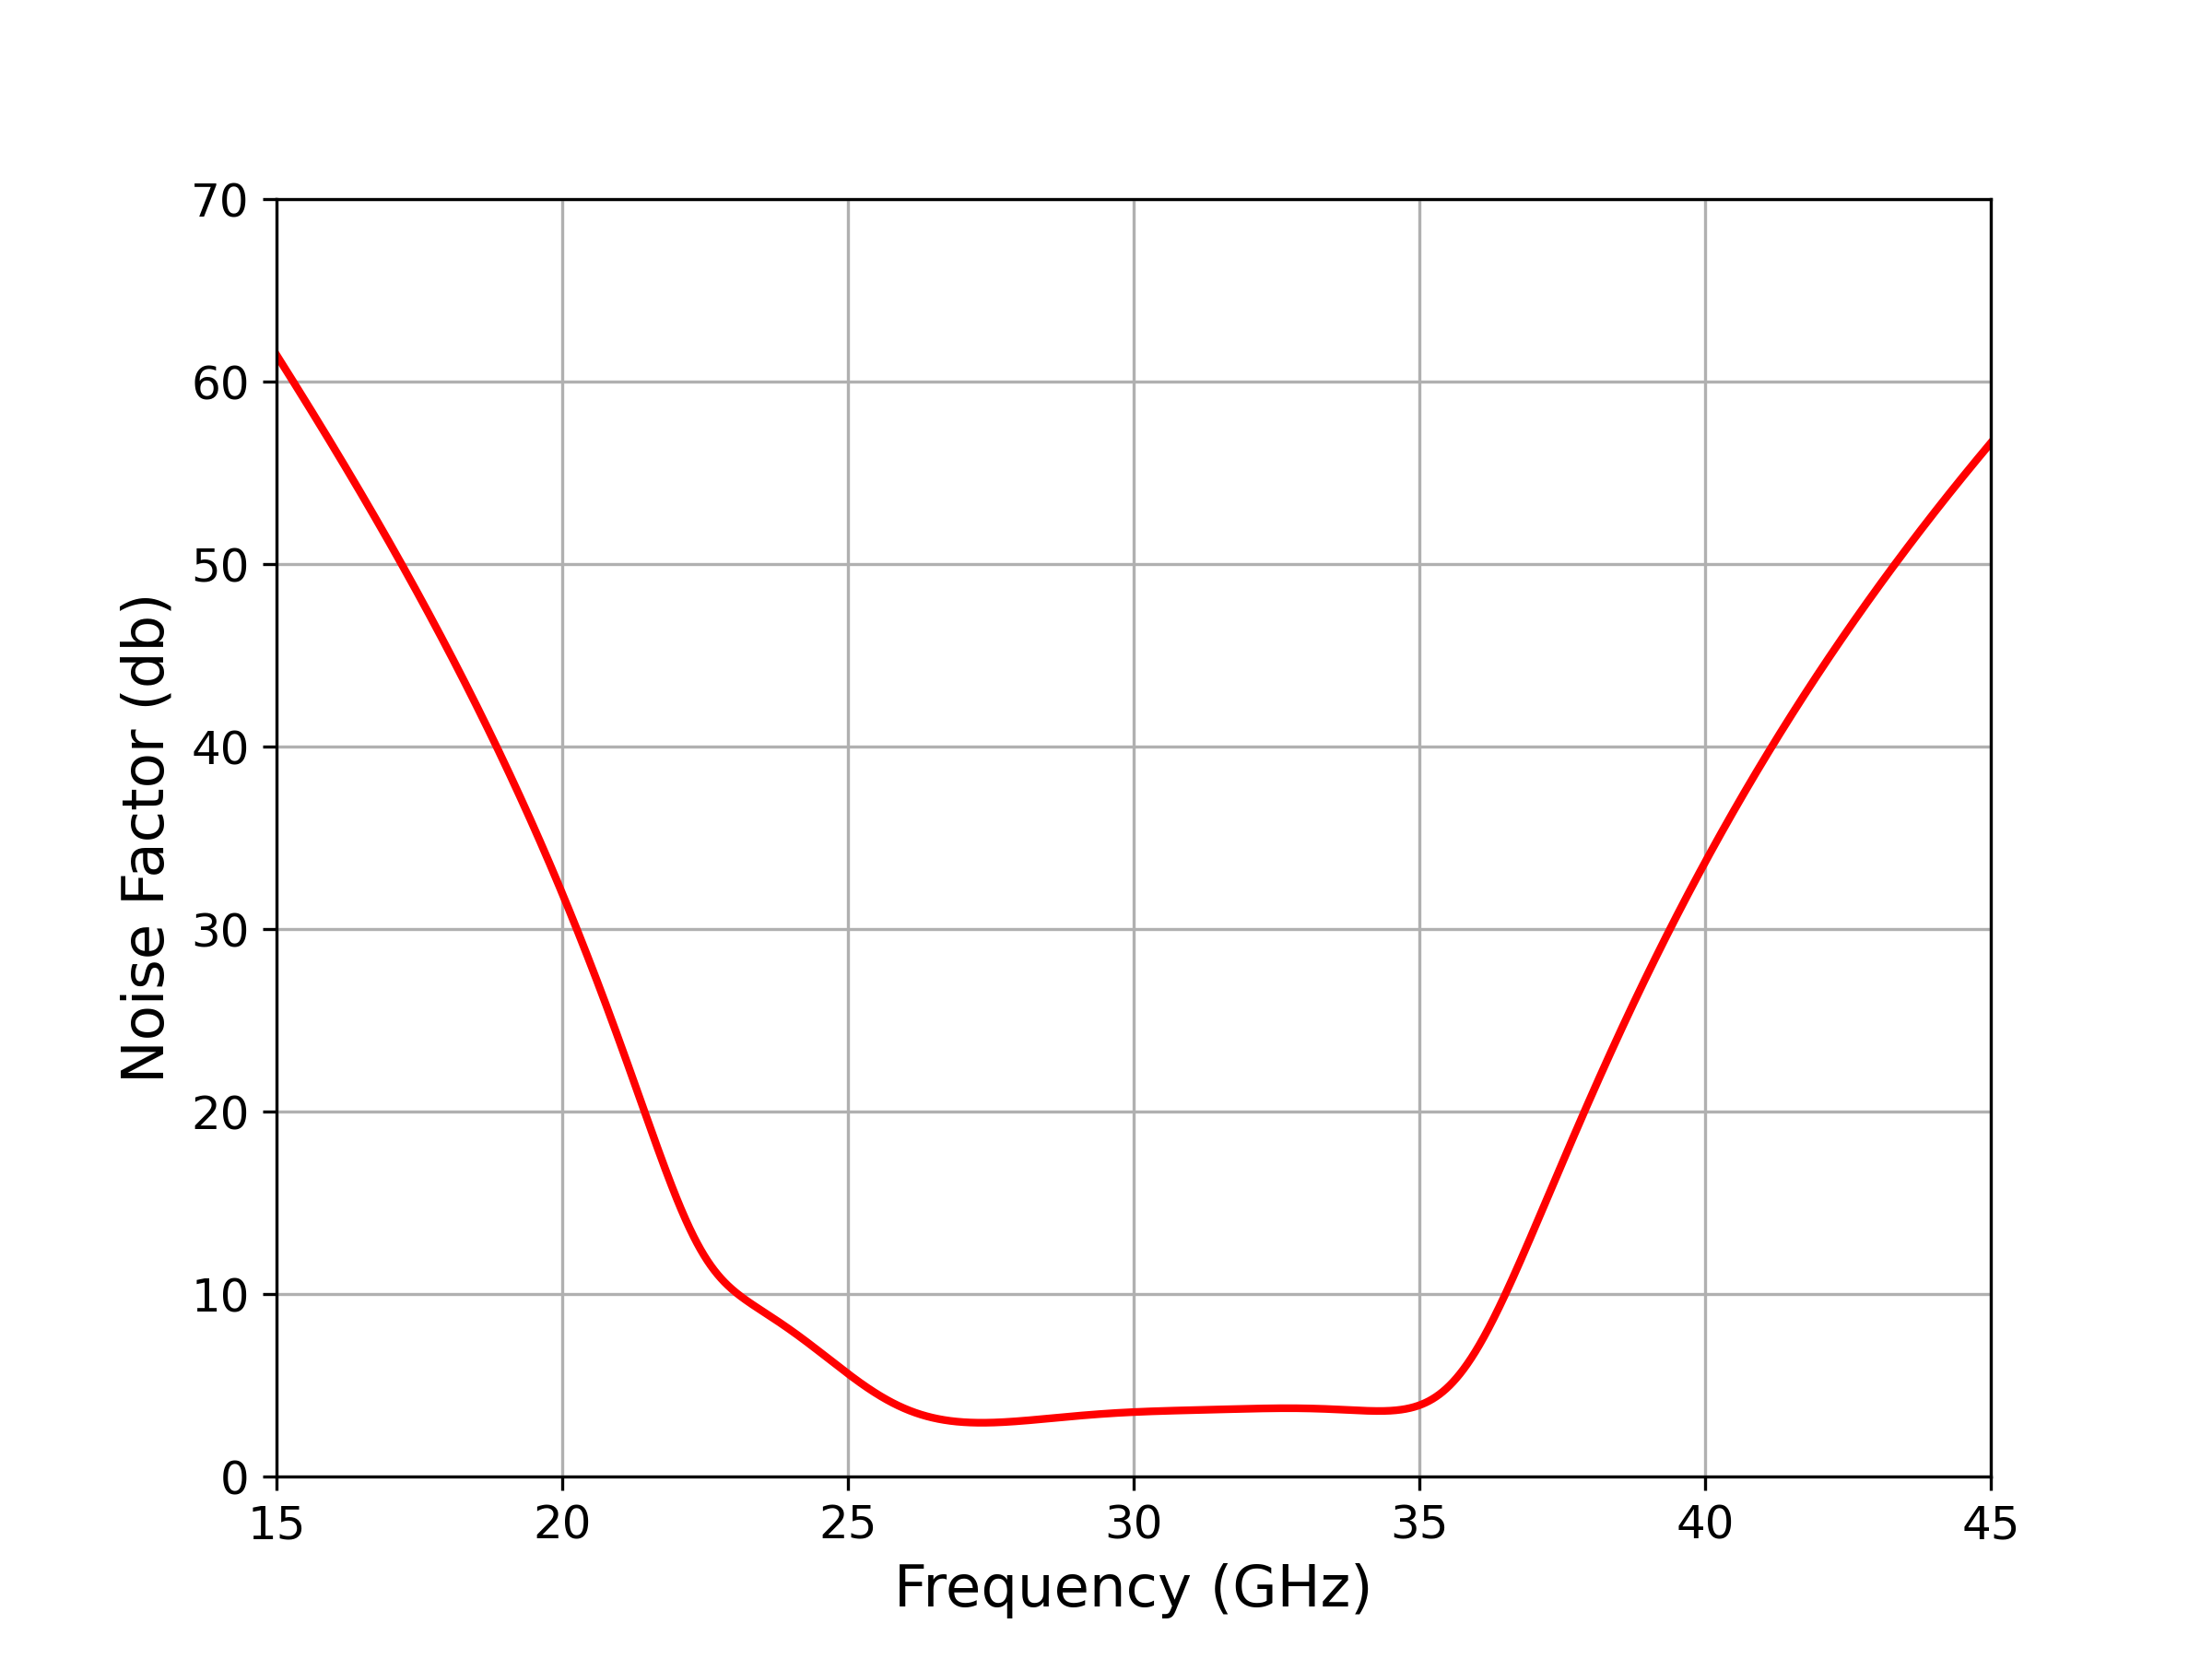
\includegraphics[]{figures/noise-factor.png}
%     }
%     \caption{Noise factor of a two-stage power amplifier (shown in Figure \ref{fig:two-stage-with-input-interstage-matching}) with input and interstage matching network.}
%     \label{fig:noise-figure}
% \end{figure}
% \begin{figure}[H]
%     \centering
%     \resizebox{0.8\textwidth}{!}{
%     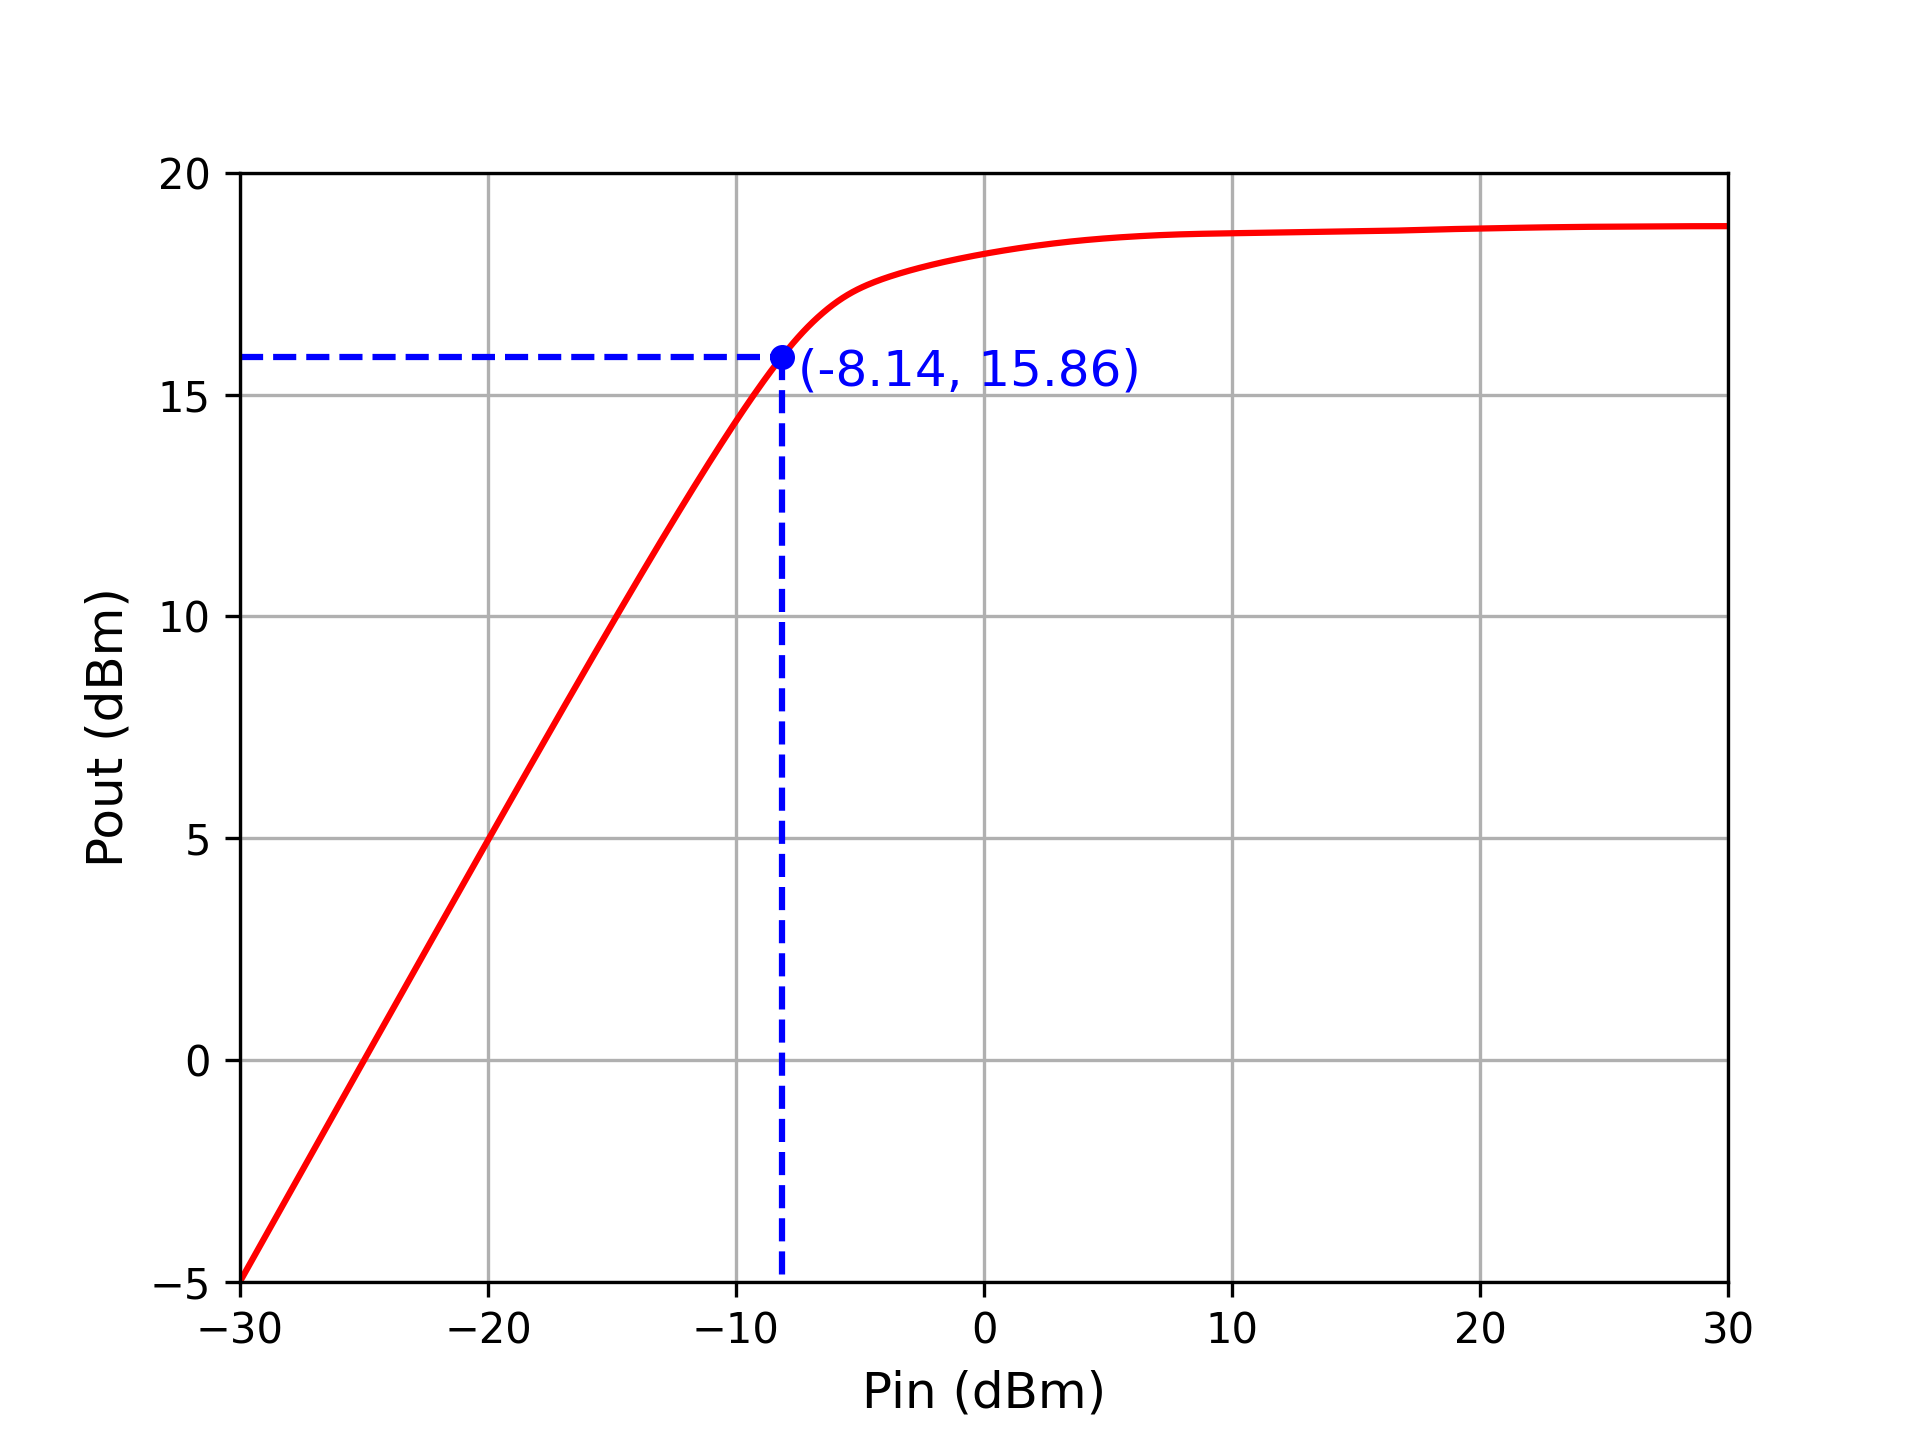
\includegraphics{figures/compressionCurves.png}
%     }
%     \caption{P1db compression curve of a two-stage power amplifier (shown in Figure \ref{fig:two-stage-with-input-interstage-matching}) with input and interstage matching network.}
%     \label{fig:compression}
% \end{figure}
\section{Analysis}
The given results describe the performance of a dual-band single-stage CMOS power amplifier circuit and its improvement through the addition of a second stage and matching networks. The key findings and implications of each stage and the matching network are given below.
\begin{enumerate}
\item Single-stage CMOS power amplifier:
The single stage CMOS power amplifier shown in Figure \ref{fig:single-stage-power-amplifier} and $S$ parameter simulation results $S_{11}$, $S_{12}$, $S_{21}$ and $S_{22}$ are shown in Figure \ref{fig:single-stage-without-cadence-s11}, \ref{fig:single-stage-without-cadence-s12}, \ref{fig:single-stage-without-cadence-s21} and \ref{fig:single-stage-without-cadence-s22} respectively.
    \begin{itemize}
       \item $S_{11}$: The value of $S_{11}$ at -0.17 dB indicates poor impedance matching at 18 GHz. This means that a significant portion of the power is being reflected back rather than absorbed by the amplifier, leading to inefficiency.
       \item $S_{21}$: The small value of 3.8 dB for $S_{21}$ indicates low power gain. This is primarily due to the parasitic capacitances and frequency-dependent transconductance of the CMOS transistors used in the amplifier circuit. These factors reduce the effective gain, especially at higher frequencies.
    \end{itemize}
\item Second stage addition:
The second stage was added using a staggered tuning technique to enhance gain and bandwidth.
The two stage CMOS power amplifier shown in Figure \ref{fig:double-stage-power-amplifier} and $S$ parameter simulation results $S_{11}$, $S_{12}$, $S_{21}$ and $S_{22}$ are shown in Figure \ref{fig:two-stage-without-cadence-s11}, \ref{fig:two-stage-without-cadence-s12}, \ref{fig:two-stage-without-cadence-s21} and \ref{fig:two-stage-without-cadence-s22} respectively.
    \begin{itemize}
        \item $S_{11}$: The value of -1.5 dB for $S_{11}$ suggests that input impedance matching has improved compared to the single-stage amplifier. However, further improvement may still be required.
        \item $S_{21}$: The power gain of 24 dB at 15 GHz indicates a significant enhancement compared to the single-stage amplifier. However, the gain decreases drastically as the frequency increases, which limits the bandwidth
    \end{itemize}

\item Matching network design:
    An input matching network and interstage matching network were designed using ADS (Advanced Design System) to improve impedance matching.
    The two stage dual band CMOS power amplifier shown in Figure \ref{fig:two-stage-with-input-interstage-matching} and $S$ parameter simulation results $S_{11}$, $S_{12}$, $S_{21}$ and $S_{22}$ are shown in Figure \ref{fig:two-stage-withmatching-cadence-s11}, \ref{fig:two-stage-withmatching-cadence-s12}, \ref{fig:two-stage-withmatching-cadence-s21} and \ref{fig:two-stage-withmatching-cadence-s22} respectively.
    \begin{itemize}
        \item $S_{11}$: The proposed PA network achieves better input matching with $S_{11}$ values of -16.38 dB at 27.12 GHz and -10.22 dB at 32.33 GHz. This indicates that a larger portion of the power is being absorbed by the amplifier rather than being reflected back.
        \item $S_{21}$: The maximum value of $S_{21}$ at 26.41 GHz is 27.55 dB, indicating a higher power gain compared to the previous stages.
        Average gain and gain at matching frequencies: The average gain across the frequency range of  25 to 35 GHz is 21.78 dB. At the matching frequencies of 27.12 GHz and 32.33 GHz, the gain values are 25 dB and 18.96 dB, respectively. These gains demonstrate the improvement achieved through the matching network.
        \item Output return loss ($S_{22}$): The proposed PA exhibits good reverse isolation with $S_{22}$ values of less than -5 dB, indicating that a small portion of the output power is reflected back.
        \item Reverse isolation ($S_{12}$) The proposed PA also exhibits good reverse isolation of -40 dB over the frequency range of 25 to 35 GHz.
    \end{itemize}
\end{enumerate}
Other important parameters:
\begin{enumerate}
\item 1 dB compression point (P1dB):
        The P1dB of the proposed PA is (-8.14 dBm, 15.86 dBm). This refers to the output power level at which the gain decreases by 1 dB from its constant value.
        Operating below the compression point is crucial to avoid non-linear behavior, distortion, and the generation of harmonics and intermodulation products.

\item $P_{sat}$:
        The $P_{sat}$ value of 12 dBm represents the maximum power level that the amplifier can handle without distortion.
        It is an important parameter for amplifier design and characterization.
\end{enumerate}
In summary, the initial single-stage CMOS power amplifier showed poor impedance matching and limited power gain. Through the addition of a second stage and the design of matching networks, improvements in input matching, power gain, bandwidth, and output return loss were achieved. The proposed PA demonstrated better performance in terms of gain, matching, and reverse isolation. However, it is important to operate the amplifier below its 1 dB compression point to avoid non-linear effects.
\newpage
\section{Performance Comparison Table}
\begin{table}[H]
  \centering
  \caption{Performance comparison with the wideband PA.}
  \label{tab:thesis_comparison_table}
  \begin{tabular}{|>{\centering\arraybackslash}m{1.5cm}|>{\centering\arraybackslash}m{1.5cm}|>{\centering\arraybackslash}m{1cm}|>{\centering\arraybackslash}m{1cm}|>{\centering\arraybackslash}m{1cm}|>{\centering\arraybackslash}m{1cm}|>{\centering\arraybackslash}m{2cm}|}
  \hline
  Ref. & CMOS Tech. & Gain (dB) & Freq (GHz) & $P_{1dB}$ (dBm) & $P_{sat}$ (dBm) & FBW (GHz) \\
  \hline
  This Work & 90 nm & 25 & 27.12 & 15.86 & 18.79 & (20.1\%) (25.66-31.1)\\
  \hline
  \cite{9829838} & 180 nm & 12.0 & 18 & 12.3 & 16.6 & (44.44\%) (14-22)\\
  \hline
  \cite{4729652} & 180 nm & 16.3 & 22 & 14.3 & 16.8 & (18.2\%) (20-24)\\
  \hline
  \cite{6634275} & 180 nm & 15.2 & 26 & 16 & 19.5 & (58.8\%) (18-33)\\
  \hline
  \cite{7890430} & 65 nm & 20.6 & 15.5 & 11.6 & 13.9 & (33.8\%) (13.5-19)\\
   \hline
   \cite{7742408} & 28 nm & 15.7 & 30 & 13.2 & 14 & (13.2\%) (27.4-32.2)\\
   \hline
   \cite{9252864} & 28 nm & 21.2 & 24 & 18.2 & 19.7 & (31.7\%) (21.8-30)\\
   \hline
  \end{tabular}
\end{table}

\chapter{CONCLUSION}
In conclusion, the study looked into CMOS power amplifier design and optimization for improved gain and bandwidth in the  25GHz to 35GHz frequency range. Due to parasitic capacitances and frequency-dependent transconductance, the first single-stage power amplifier design had trouble matching input impedances and had lower gain. However, the cascaded power amplifier showed increased gain performance at a lower frequency by adding a second stage and using a staggered tuning strategy. In order to achieve better impedance matching, the design also included matching networks, which led to increased gain and decreased return loss. Gain, bandwidth, and matching performance of the power amplifier were successfully increased by the optimization efforts.

The proposed PA design impedance matched at two points: 27.12 GHz and 32.32 GHz compared to whole 25-35 GHz. That means the impedance hasn’t matched perfectly throughout the bandwidth. So, there is scope of designing the impedance matching network perfectly in future. Due to the presence of parasitic capacitance, there are some oscillations in the magnitude of $S_{21}$ parameter (power gain). We have to minimize the value of the parasitic capacitance of the power amplifier to reduce the oscillation in power gain curve.
\section{Future Work}
\begin{enumerate}
    

\item Explore Higher CMOS Technologies:
 The thesis paper focuses on designing CMOS power amplifiers using 90 nm CMOS technology. In the future, it would be beneficial to investigate the performance of power amplifiers using more advanced CMOS technologies, such as 65 nm, 45 nm, 28 nm or even smaller nodes. This would allow for higher integration levels, improved performance, and potentially reduced power consumption.

\item Investigate Different Circuit Topologies:
 The thesis paper may have focused on a specific circuit topology for power amplifiers. In the future, it would be interesting to explore different circuit architectures, such as Class F, Class G, or Class H, to determine their suitability for enhanced gain and bandwidth. Each circuit topology has its own advantages and limitations, so studying alternative options could provide valuable insights.

\item Implement Advanced Techniques for Bandwidth Enhancement:
 The thesis paper has employed staggered tuning technique using 2 stage power amplifier to enhance the bandwidth of the CMOS power amplifiers. Future work could involve investigating and implementing more advanced techniques like harmonic tuning, active inductors, or advanced matching networks to further improve the bandwidth performance.

\item Study Power Amplifier Linearity: 
The thesis paper may have primarily focused on gain and bandwidth enhancements. However, power amplifier linearity is another crucial aspect to consider, especially for applications where the amplifier needs to handle high-power signals. Future research could focus on studying linearity improvement techniques, such as linearization circuits or predistortion techniques, to achieve enhanced linearity while maintaining high gain and wide bandwidth.
\end{enumerate}
Overall, the research outcomes demonstrate the potential for enhancing CMOS power amplifier performance in wideband applications. By addressing the limitations and implementing design improvements, it is possible to achieve higher gain, wider bandwidth, and better impedance matching. The proposed recommendations pave the way for future research and development in this field, enabling the realization of high-performance CMOS power amplifiers for next-generation wideband communication systems.


\bibliography{references}
\bibliographystyle{ieeetr}
%\bibliographystyle{IEEEtran}
%\bibliographystyle{plainnat}
\end{document}
